\chapter{Adaptive LES of Flow Over Surging Airfoil}

In this chapter, we first investigate the three different mesh adaptation strategies based on the VMS-based estimated error to perform adaptive large eddy simulation of flow over a surging airfoil.
The zonal-based strategy is found to be most effective. This strategy is subsequently applied for adaptive LES, at two Reynolds numbers of $Re=40,000$ and $200,000$, to construct a series of adapted meshes for which mesh convergence is shown. In particular, for quantities of interest including pressure coefficient and leading edge vortex (LEV) evolution.
% A brief overview of the three strategies considered is mentioned in chapter \ref{sec:adapt_strat_overview}.

\section{Problem Setup}

The problem setup for these cases is the same as the one described in Section \ref{sec:problem_setup_baseline}.

\section{Summary of Cases}

In this chapter, NACA 0012 airfoil is considered at Reynolds number of $Re=40,000$ and $200,000$, and at a sectional advance ratio of $\mu_{sect}=1.2$ (i.e., higher value), see Table \ref{table:adapt_summary_cases}. Note that for the $Re=1,000,000$ case, the computational cost is significantly higher and it exhibits a similar flow behavior as the $Re=200,000$ case, especially in LEV evolution. Thus, $Re=40,000$ and $200,000$ are considered in this chapter for adaptive LES. Similarly, only higher advance ratio of $\mu_{sect}=1.2$ is considered for adaptive LES (since it shows more complex flow behaviour as compared to the lower advance ratio of $\mu_{sect}=1.0$).

\begin{table}[H]
	\centering
	\caption{Summary of surging cases for adaptive LES}
	\label{table:adapt_summary_cases}
	\begin{tabular}{|l|c|c|c|c|}
		\hline
		Airfoil   & $\alpha$ & $k$ & $\mu_{sect}$ & $Re$ \\
		\hline
		\hline
		NACA 0012 & 6$^\circ$ & $0.133$ &  1.2 & \{40,000,\; 200,000\} \\
		% \hline
		% NACA 0012 & 6$^\circ$ & $0.133$ & 1.2 & 200,000 \\
	\hline
	\end{tabular}
\end{table}

First, three different adaptive strategies are studied for the lower Reynolds number of $Re=40,000$, in which zonal-based strategy is found to be most effective. Subsequently, zonal-based strategy is used for both Reynolds numbers of $Re=40,000$ and $200,000$ to create a series of adapted meshes and show mesh convergence for adaptive LES.

% Next, adaptive LES is performed for $Re=40,000$ and $Re=200,000$ cases, where a series of adapted meshes is constructed, and mesh convergence is shown.

\section{Application and Comparison of Different Adaptive Strategies}
\label{sec:adaptive_strategy_comparison}
\chapter{Adaptive Strategies}

In this section, we focus on adaptive LES of flow over a surging airfoil at different conditions. Problem setup, and baseline results including vortex detection and tracking, are first presented using the non-adapated mesh. We also present active flow control cases in the form of active reflex camber. Next, we present the three adaptive strategies and corresponding results. 

\chapter{LES of Flow Over Surging Airfoil}
\label{chapter:baseline_results}

In this chapter, we focus on LES of flow over a surging airfoil at different conditions. Problem setup as well as results including vortex detection and tracking are presented. A non-adapated mesh is used here to get familiar with the features of the current problem at different conditions, while results on the adapted meshes are presented in the next chapter.
% We also present active flow control cases in the form of active reflex camber. 

%\section{LES of Flow Over Surging Airfoil}
%\section{Adaptive LES of Flow Over Surging Airfoil}
%\section{LES of Flow Over Surging Airfoils including Active Reflex}


\section{Problem Setup}
\label{sec:problem_setup_baseline}

%TODO: Add U_rel velocity profile with t_tilde

A schematic of the problem setup is shown in Figure~\ref{fig:SetUpSketch}, where $U_\infty$ is the free-stream or mean velocity and $\alpha$ is the angle of attack.

\begin{figure}[H]
\centering
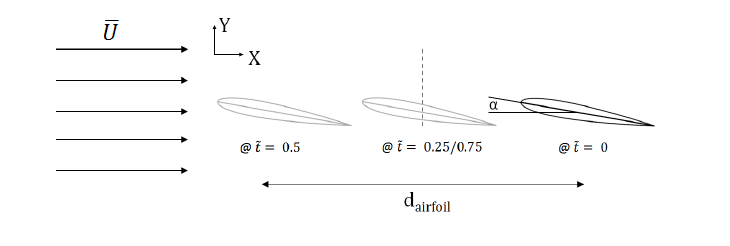
\includegraphics[width=0.8\textwidth]{figures/Setup/Setup.png}
\caption{Schematic of the surging airfoil problem}
\label{fig:SetUpSketch}
\end{figure}

The airfoil motion is set as follows
\begin{equation}
\label{eq:displacement}
  d_{airfoil} = A cos(2\pi f t) =  Acos(2\pi t/T) = Acos(2\pi\tilde{t})
\end{equation}

\noindent where $A$ is the amplitude and $T=1/f$ is the time period of the oscillation.
The variable $\tilde{t}$ is the fractional part in the oscillation cycle and is defined as $\tilde{t}=\{t/T\} = t/T - \lfloor t/T \rfloor$ (where $\lfloor \cdot \rfloor$ is the floor function).

The (non-dimensional) relative velocity is expressed as
\begin{equation}
\label{eq:relVelocity}
  \tilde{U}_{rel} = U_{rel}/U_\infty = 1 - U_{airfoil}/U_\infty = (1+\mu_{sect} sin(2\pi\tilde{t}))
\end{equation}
\noindent where $\mu_{sect}$ is the sectional advance ratio.
Note that for a sectional advance ratio above $1.0$ a negative relative velocity or a reversed flow condition is attained (e.g., at this radial section/location of the blade).
Under the reversed flow condition the relative flow is from the (geometric) trailing edge to the leading edge of the airfoil.

At $\tilde{t}$=0, with $\psi$=$0^\circ$ or $\psi$=$0^\circ$ (where, $\psi$ is the phase in the oscillation cycle and $\psi$ is the azimuthal position of the blade), the relative velocity is the free-stream velocity (i.e., $U_\infty$).
The same holds at $\tilde{t}$=0.5 or $\psi$=$180^\circ$.
At $\tilde{t}$=0.25 or $\psi$=$90^\circ$, the airfoil is at the maximum relative velocity and at $\tilde{t}$=0.75 or $\psi$=$270^\circ$ is at the minimum relative velocity.
Advancing part of the cycle is defined between $\tilde{t}$=0 or $\psi$=$0^\circ$ and $\tilde{t}$=0.5 or $\psi$=$180^\circ$, while retreating part is between $\tilde{t}$=0.5 or $\psi$=$180^\circ$ and $\tilde{t}$=1.0 or $\psi$=$360^\circ$ (or back to $\psi$=$0^\circ$).

The free-stream or mean Reynolds number is defined as: $Re=U_\infty C/\nu$, where $C$ is the chord.
The reduced frequency is defined as $k=\pi f C/U_\infty$ while the amplitude is related as $A = \frac{\mu_{sect} C}{2k}$.

\section{Summary of Cases}
\label{sec:baseline_case_summary}

In the current study, the reduced frequency is held fixed at $k$=0.133 while three Reynolds numbers of $Re$=40,000, 200,000 and 1,000,000 are considered together with two sectional advance ratios of $\mu_{sect}$=1.0 and 1.2, i.e., six cases are considered in total.
The angle of attack of the airfoil is set to 6$^\circ$.
Note that we considered the Reynolds number of $Re$=40,000 in a previous study~\cite{bib:kocher_scitech2017} that was selected in accordance with the experiments conducted in \cite{bib:granlund2016} where the airfoil was placed in a constant flow and oscillated in the streamwise direction.
The six cases are summarized in Table~\ref{table:summary_cases}.

\begin{table}[H]
\centering
\caption{Summary of cases}
\label{table:summary_cases}
\begin{tabular}{|l|c|c|c|c|}
\hline
Airfoil   & $\alpha$ & $k$ & $\mu_{sect}$ & $Re$ \\
\hline
\hline
NACA 0012 & 6$^\circ$ & $0.133$ & \{1.0, 1.2\} & \{40,000,\; 200,000,\; 1,000,000\} \\
\hline
\end{tabular}
\end{table}

The computational domain is set to be $100C$ x $50C$ x $0.2C$.
At the inlet, a constant free-stream velocity is applied
(note that the airfoil is moved sinusoidally in the streamwise direction).
No-slip condition is prescribed on the moving airfoil.
The top and bottom surfaces are set as slip walls.
Side surfaces in the spanwise direction (i.e., front and back surfaces) are imposed to be periodic.
A natural pressure condition is used at the outlet.
A second-order implicit time integration scheme, e.g., see \cite{bib:tran2017b}, is employed with about 1,440 steps in an oscillation cycle.

%TODO: give justification for this mesh ... typical LES resolution for a BL (based on highest Reynolds number in the surge cycle) ... but indicate no consideration taken for other flow features such as separation and LEV.
An unstructured hybrid/boundary layer mesh is used.
The mesh is comprised of hex and wedge elements which is generated by first generating a mesh on the front surface and by subsequently applying an extrusion in the spanwise direction. This (non-adapted) mesh is used for all cases listed above. Again, this is done to get familiar with the features of the current problem at different conditions, while mesh adaptivity is investigated in the next chapter. The non-adapted mesh is constructed by following recommended practices in terms of mesh resolution on the surface of the airfoil and around it, as discussed below.

Refinement zones are placed around the airfoil to resolve the flow structures of interest, see Figure \ref{fig:mesh} (where three refinement zones are noted).
In the finest refinement zone (Z1), mesh size is set to be $C/256$.
In the subsequent two zones (Z2 and Z3), it is set to be $C/128$ and $C/64$, respectively.
In the spanwise direction, 50 extruded elements are used.
A layered and graded mesh (with geometric growth) is used around the airfoil surface, see Figure \ref{fig:mesh2}.
The first layer height is set to be $\mathcal{O}(10^{-5} C)$ such that it is below 1 in wall units for all cases.
Similarly, mesh spacing on the airfoil surface in the streamwise and spanwise directions is set to be below 80 and 50 in wall units, respectively, for the XXX (which Reynolds number and which part of the cycle).
Overall the mesh contains about 6.2 million nodes and 10.8 million elements.

\begin{figure}[H]
\centering
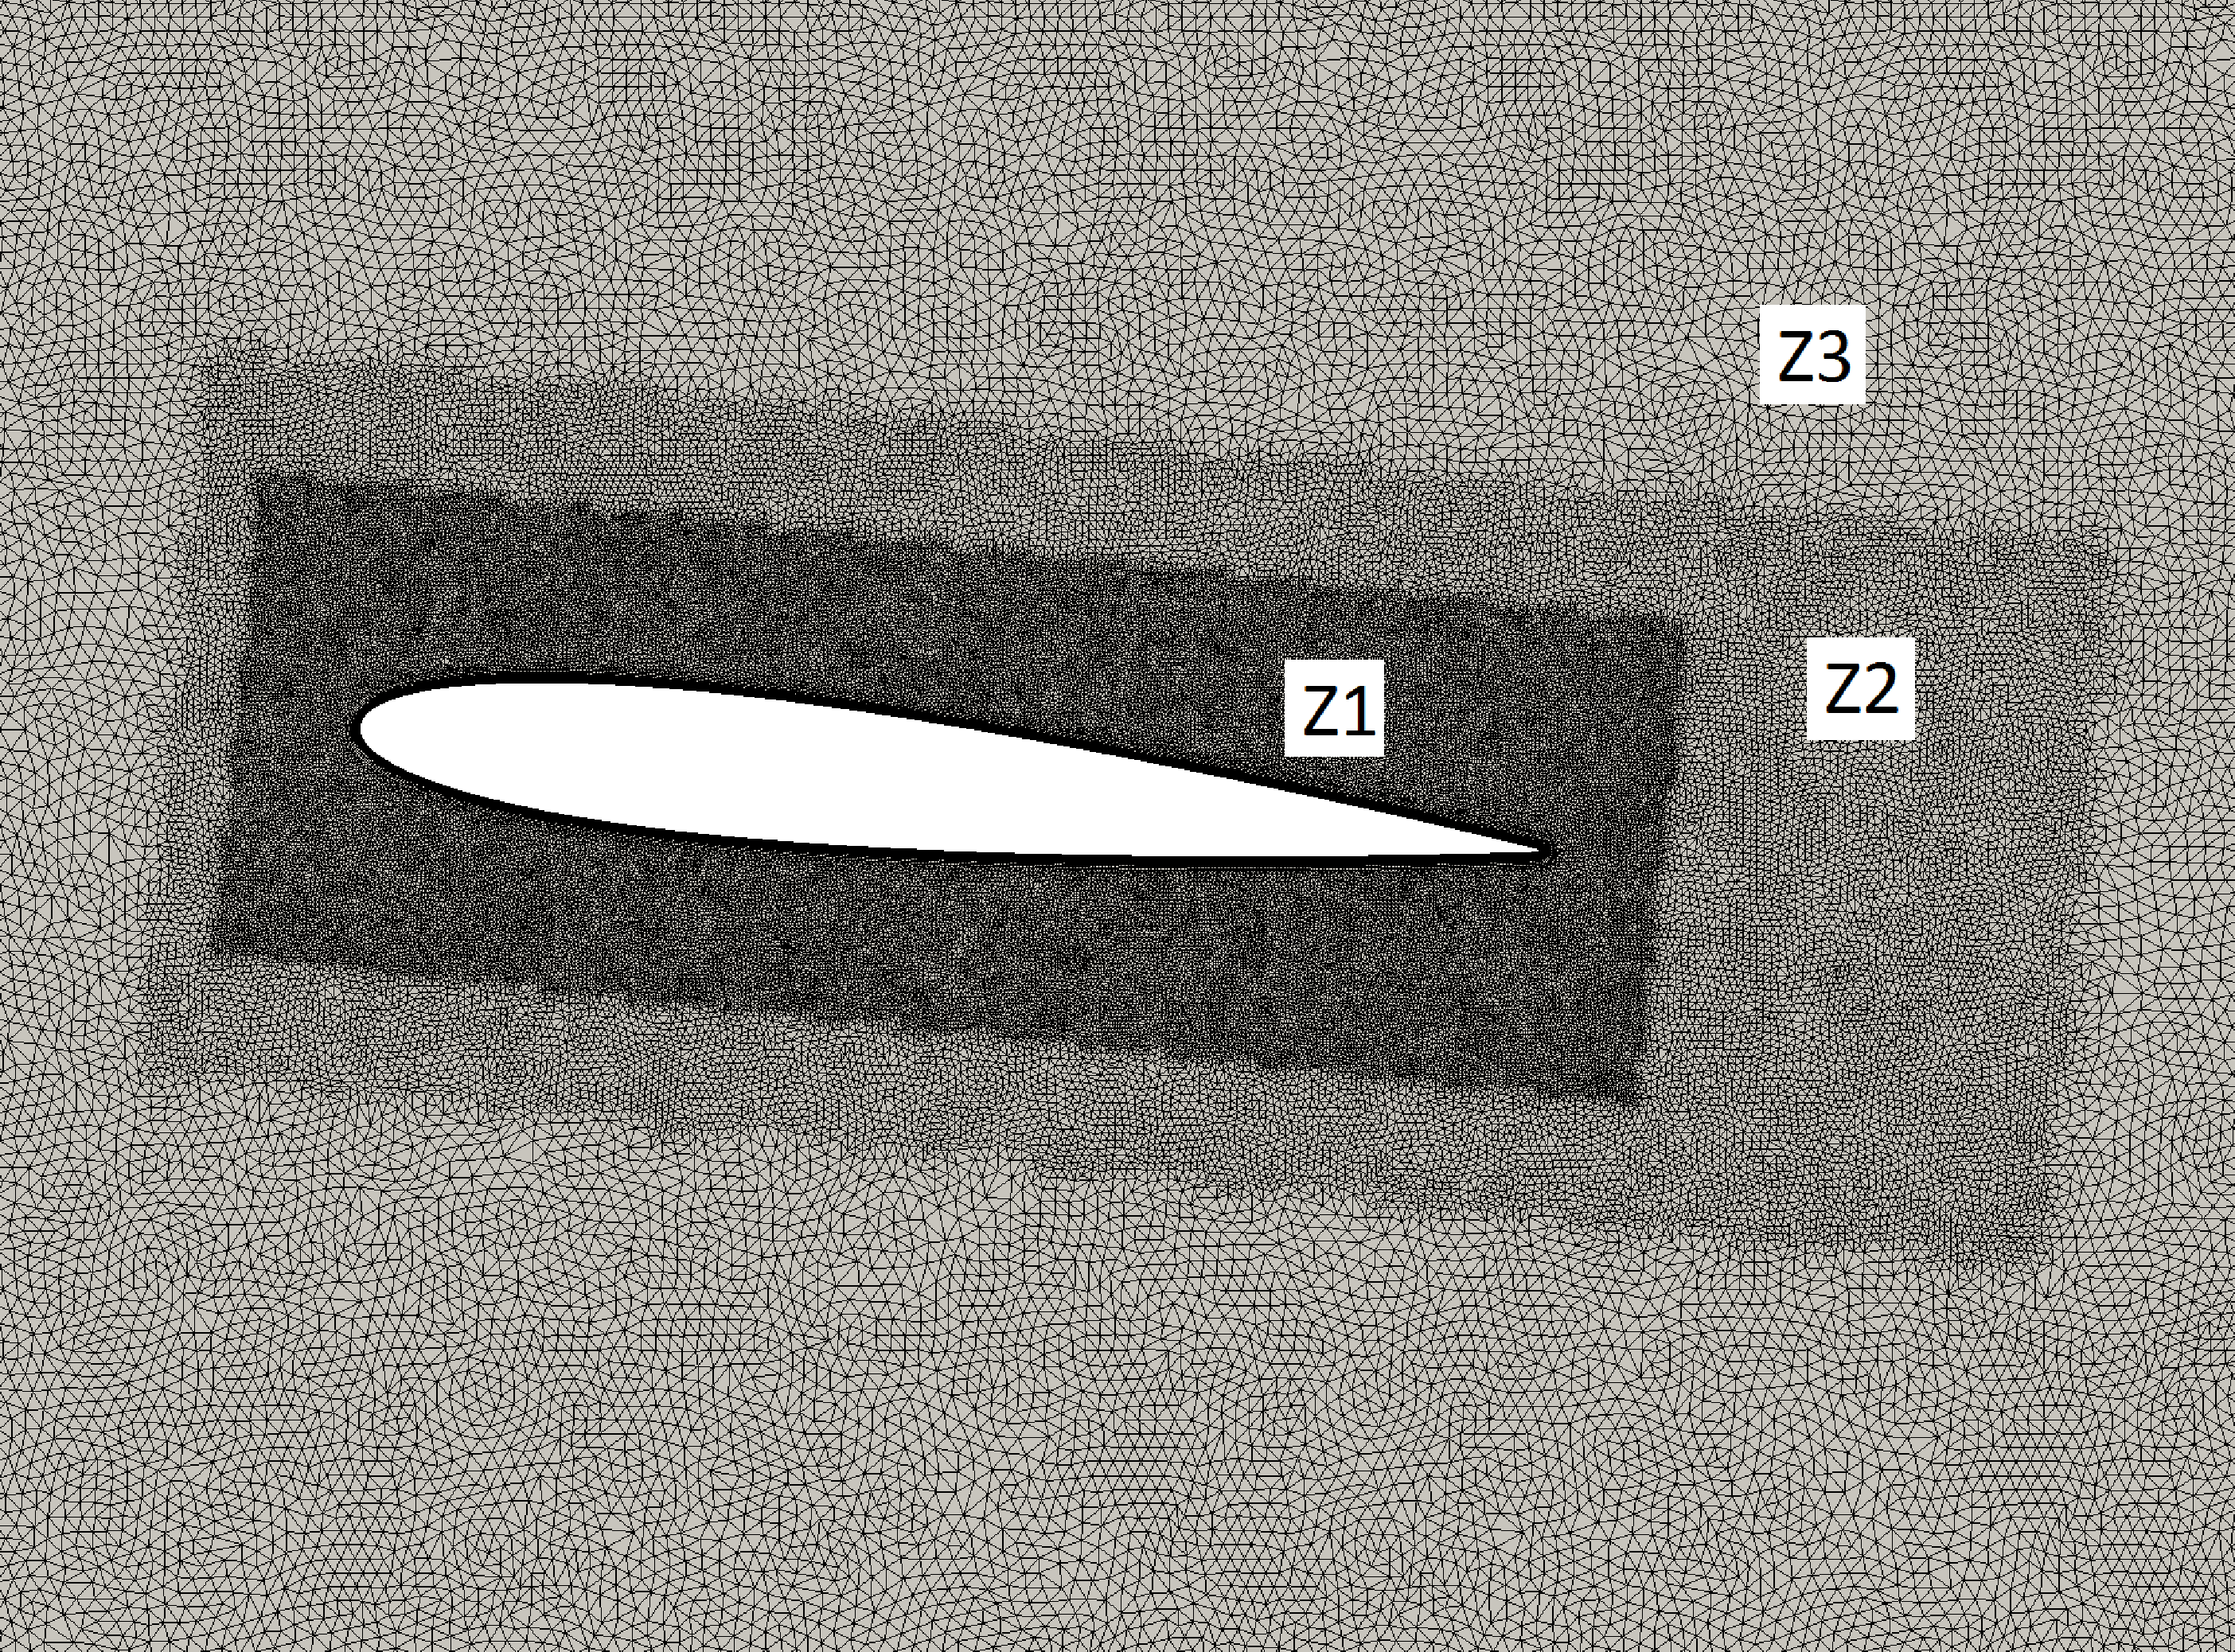
\includegraphics[width=0.7\textwidth]{figures/Setup/mesh_screenshot.pdf}
\caption{Mesh around the airfoil with refinement zones}
\label{fig:mesh}
\end{figure}

\begin{figure}[H]
\centering
\includegraphics[width=0.45\textwidth]{figures/Setup/mesh_LE.pdf}
\includegraphics[width=0.45\textwidth]{figures/Setup/mesh_TE.pdf}
\caption{Layered and graded mesh around the leading edge and trailing edge of the airfoil}
\label{fig:mesh2}
\end{figure}

\section{Results and Discussion}

\subsection{Force Response}

\begin{figure}[H]
	\begin{subfigure}{0.5\textwidth}
		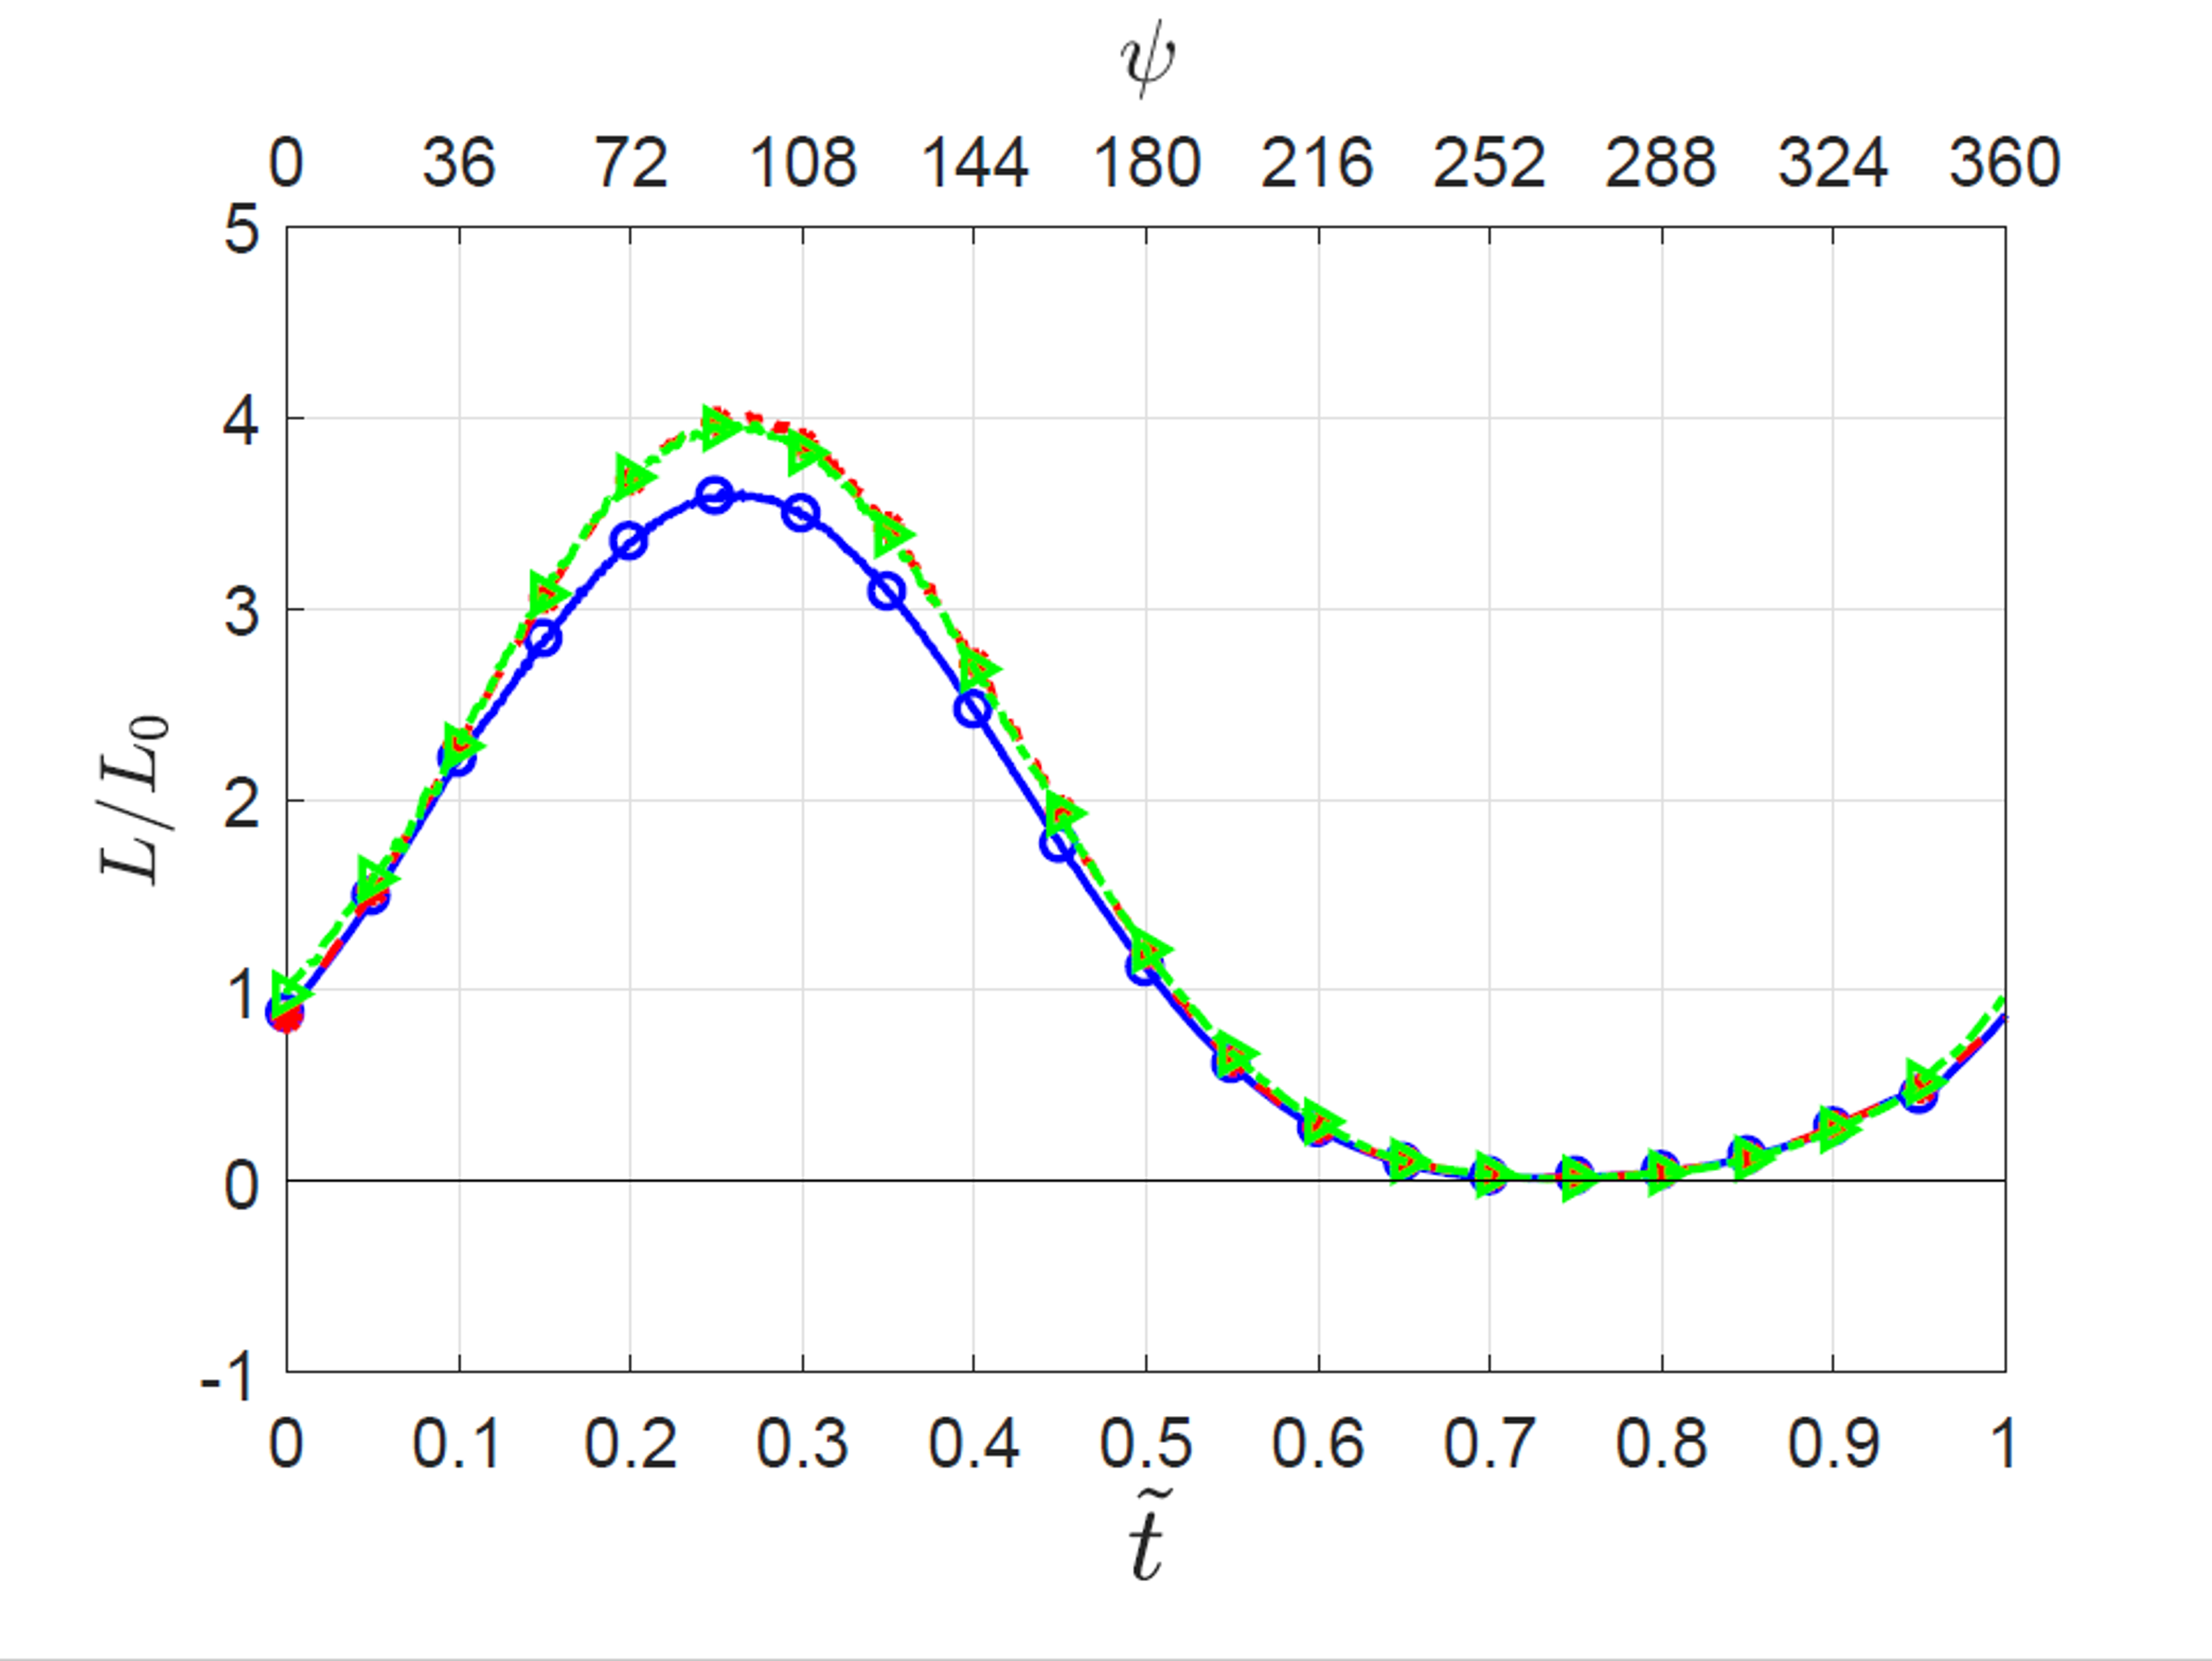
\includegraphics[width=1\textwidth]{figures/lift_Re_effect_lambda_1pt0.png}
		\subcaption{$\mu_{sect} = 1.0$}
		\label{fig:lift_Re_comparision_lambda_1p0}
	\end{subfigure}
 	\begin{subfigure}{0.5\textwidth}
		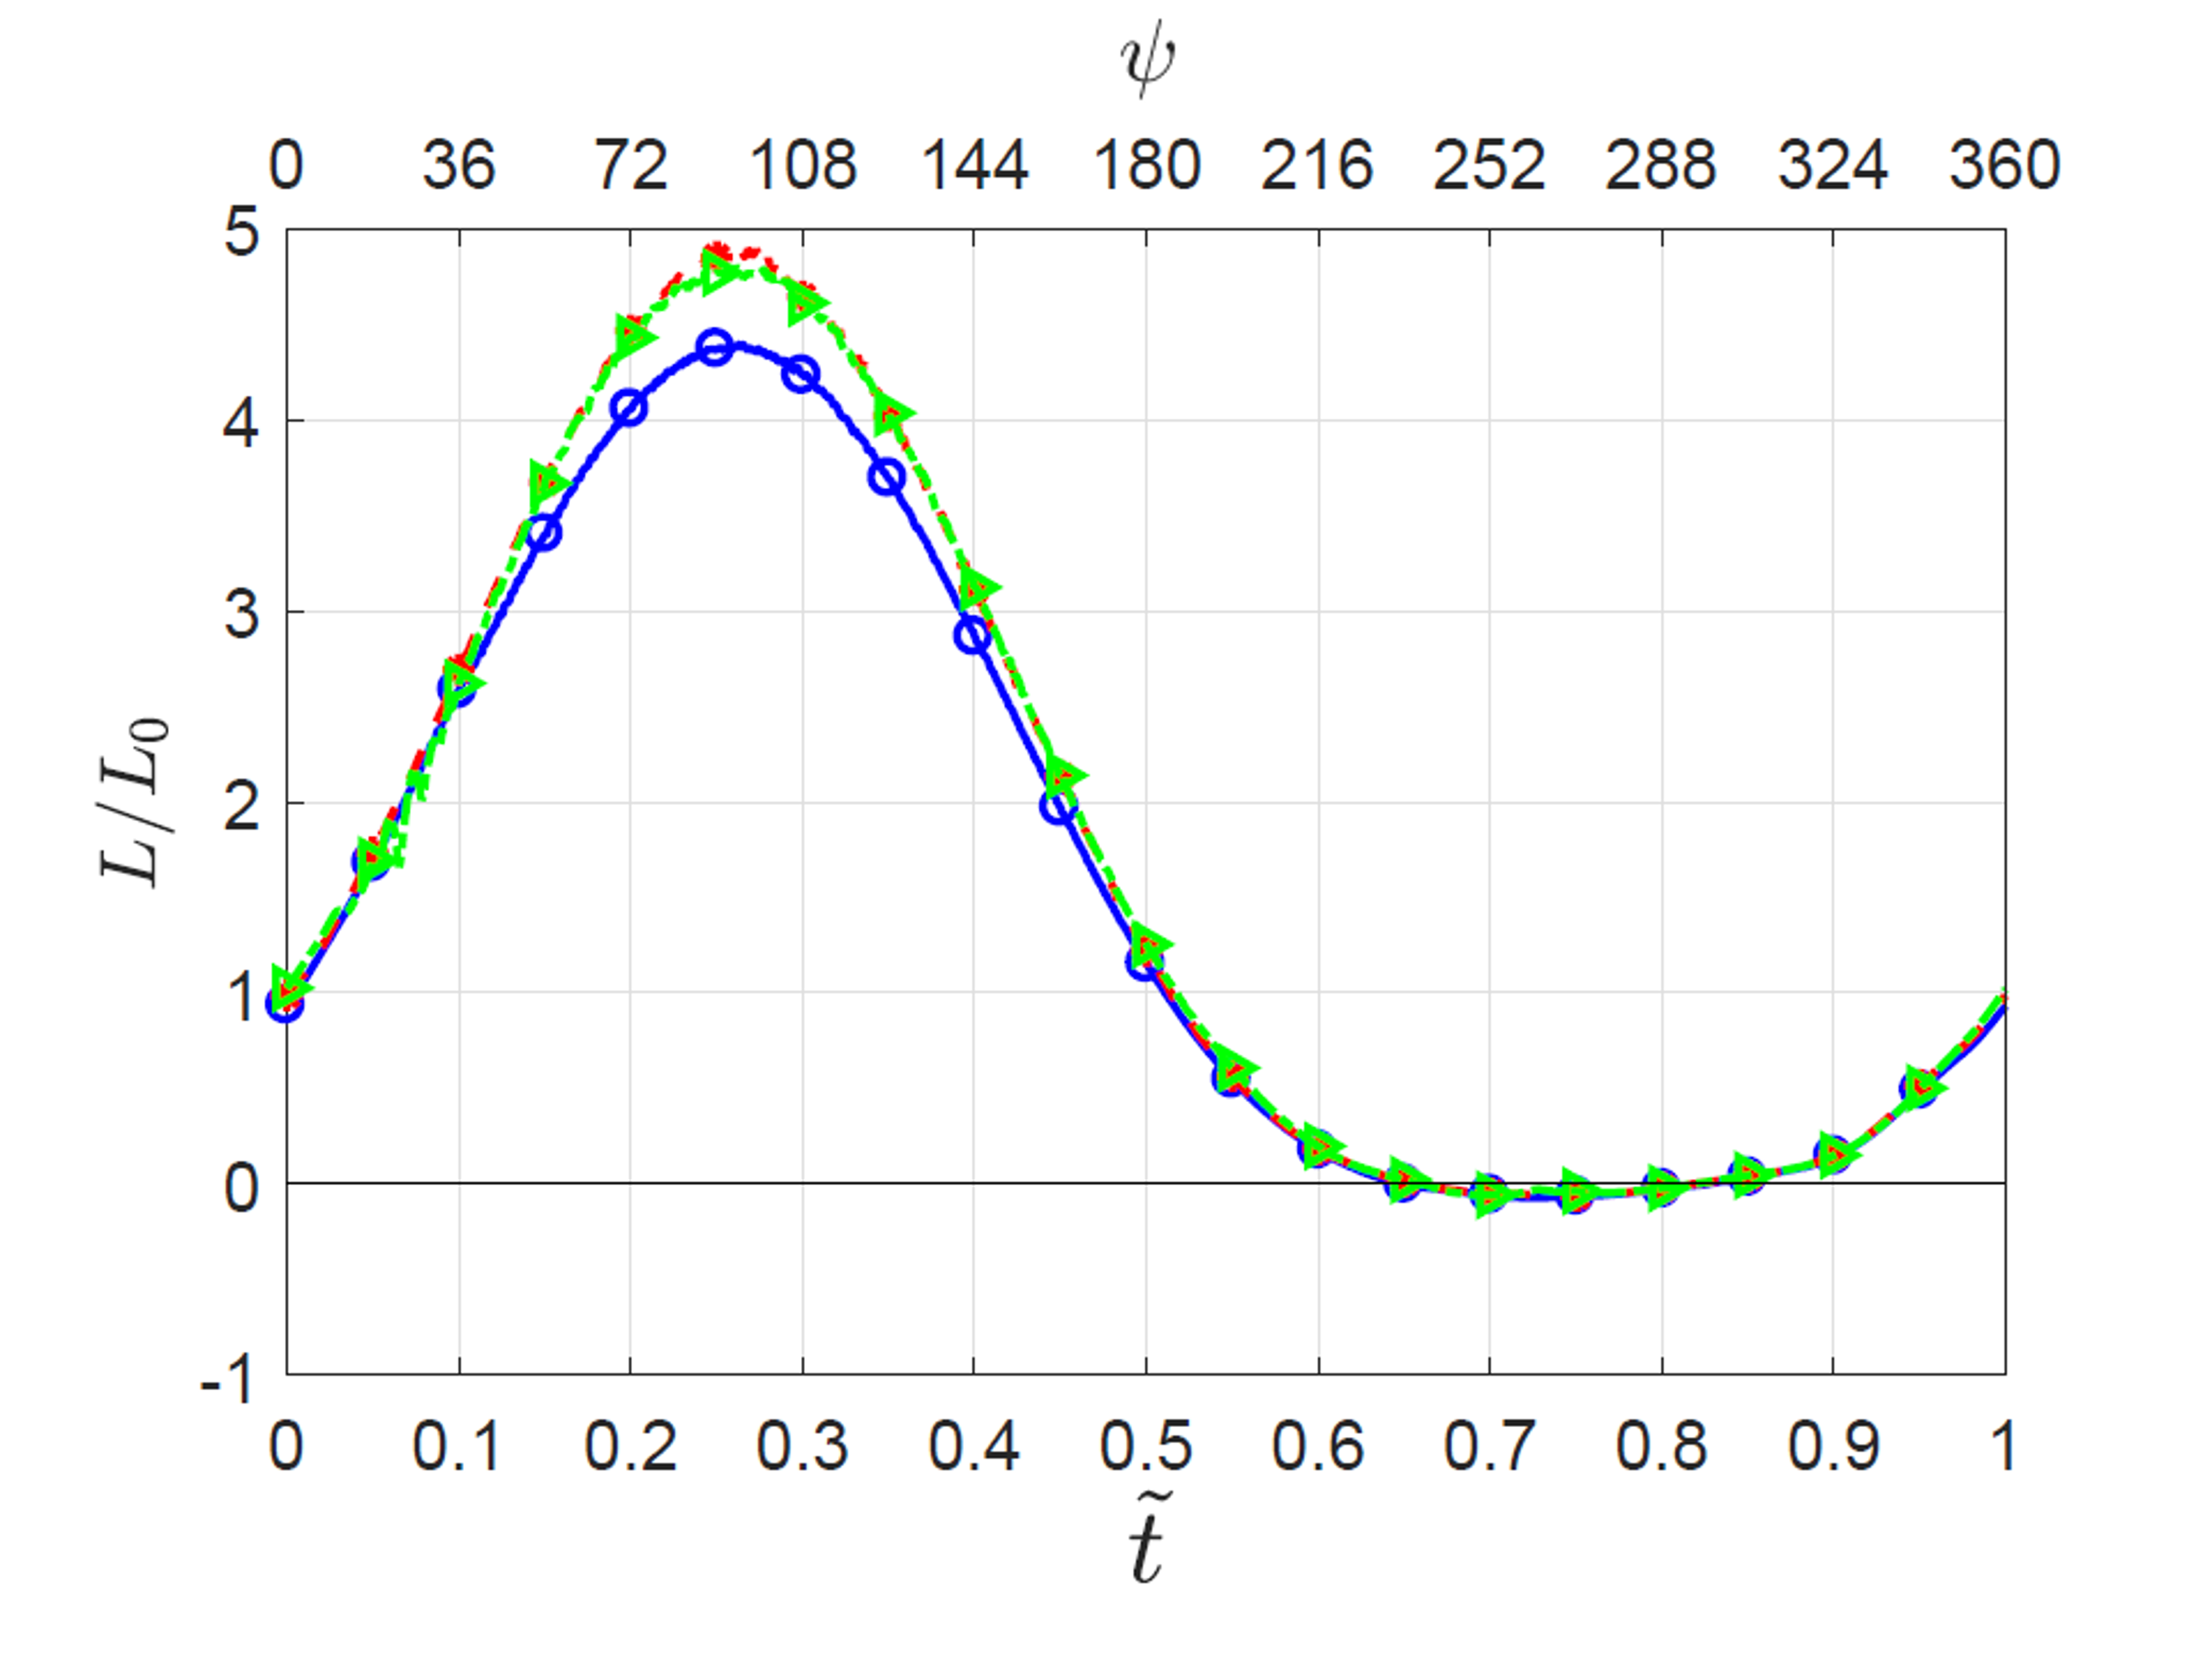
\includegraphics[width=1\textwidth]{figures/lift_Re_effect_lambda_1pt2.png}
        \subcaption{$\mu_{sect} = 1.2$}
		\label{fig:lift_Re_comparision_lambda_1p2}
	\end{subfigure}

 	\caption{Normalized lift force for $Re$=40,000 (green line with open triangles), 200,000 (red line with solid circles) and 1,000,000 (blue line with open circles) at $\mu_{sect}$=1.0 and 1.2}
 	\label{fig:lift_comparison}
\end{figure}

Lift force is shown in Figure \ref{fig:lift_comparison}.
Lift is normalized by its static counterpart, i.e., $L_0$ is the average or steady lift for the static airfoil at the mean Reynolds number over the surging cycle.
This normalization was used in our previous study with $Re$=40,000~\cite{bib:kocher_scitech2017} to compare against the experimental data of \cite{bib:granlund2016}, where a good agreement was shown between the experimental and simulation data.
Data is phase averaged over 4 cycles.
%%%We note that the averaged drag data exhibits fluctuations which is due to the presence of a turbulent flow, especially during the advancing phase of the cycle with a higher relative velocity or Reynolds number.
%%%However, these fluctuations are marginal in nature and averaging over additional cycles will be useful.

Overall, the lift force follows a similar qualitative trend for all the cases.
Maximum lift is achieved at $\tilde{t}=0.25$, which is expected as the airfoil achieves maximum relative velocity at that point.
After $\tilde{t}=0.25$, the lift starts decreasing as the airfoil begins to decelerate and enters the retreating phase. 
The lift keeps decreasing till about $\tilde{t}=0.65$ and plateaus or reaches a value close to zero during the middle of the retreating phase (i.e., around $\tilde{t}=0.75$ when the airfoil is at its minimum relative velocity).
We note that for both advance ratios of $\mu_{sect}$=1.0 and 1.2 a zero relative velocity is attained and for the higher advance ratio of $\mu_{sect}$=1.2 the relative velocity also becomes negative.
Lift starts to recover after $\tilde{t}=0.75$ as the airfoil starts accelerating again.
For each advance ratio, the normalized lift during the advancing phase for $Re$=1,000,000 is slightly smaller compared to the other two Reynolds numbers, see Figure \ref{fig:lift_Re_comparision_lambda_1p0} or Figure \ref{fig:lift_Re_comparision_lambda_1p2}.
The normalized lift is very similar between $Re$=40,000 and 200,000 cases.
The peak normalized lift is about 9\% lower for the highest Reynolds number case as compared to the lower Reynolds number cases for each advance ratio.
On the other hand, for a given Reynolds number the normalized lift is higher for the higher advance ratio, which is expected due to the higher dynamic pressure in any given instance or phase in the surging cycle.
The peak normalized lift is about 21\% higher for the higher advance ratio case as compared to the lower advance ratio case for each Reynolds number, which is the difference in the peak dynamic pressure between the two advance ratios.

\subsection{Flowfield: Spanwise Vorticity}

In this section, we present spanwise vorticity over the cycle at 8 different phases of $\psi$ = $195^\circ$, $225^\circ$, $240^\circ$, $255^\circ$, $270^\circ$, $315^\circ$, $330^\circ$,and $345^\circ$, which are all in the retreating part of the surging cycle.
We focus our attention on the leading edge vortex (LEV) which is the dominant flow feature.
It forms and advects during the retreating part, while in the advancing part the flow remains attached.
As noted earlier, data is phase averaged over 4 cycles.
In addition, averaging is also applied in the spanwise direction.

Figure \ref{fig:vortScreen_1pt0} shows the spanwise vorticity for the lower advance ratio of $\mu_{sect}$=1.0.
The voriticy range is selected to be [-10,10]$\times U_\infty /C$.
At $\psi$=$195^\circ$, the flow over the airfoil is mostly attached, however, the boundary layer is relatively thick as the airfoil is decelerating, see Figures~\ref{fig:Re_40k_1pt0_phi195}, \ref{fig:Re_200k_1pt0_phi195} and \ref{fig:Re_1m_1pt0_phi195}.
As expected, the boundary layer is much thicker for the lowest Reynolds number of $Re$=40,000 as compared to the other two higher Reynolds numbers.

\begin{figure}[H]
	\centering
	
	\begin{subfigure}[b]{0.32\textwidth}
		\centering
		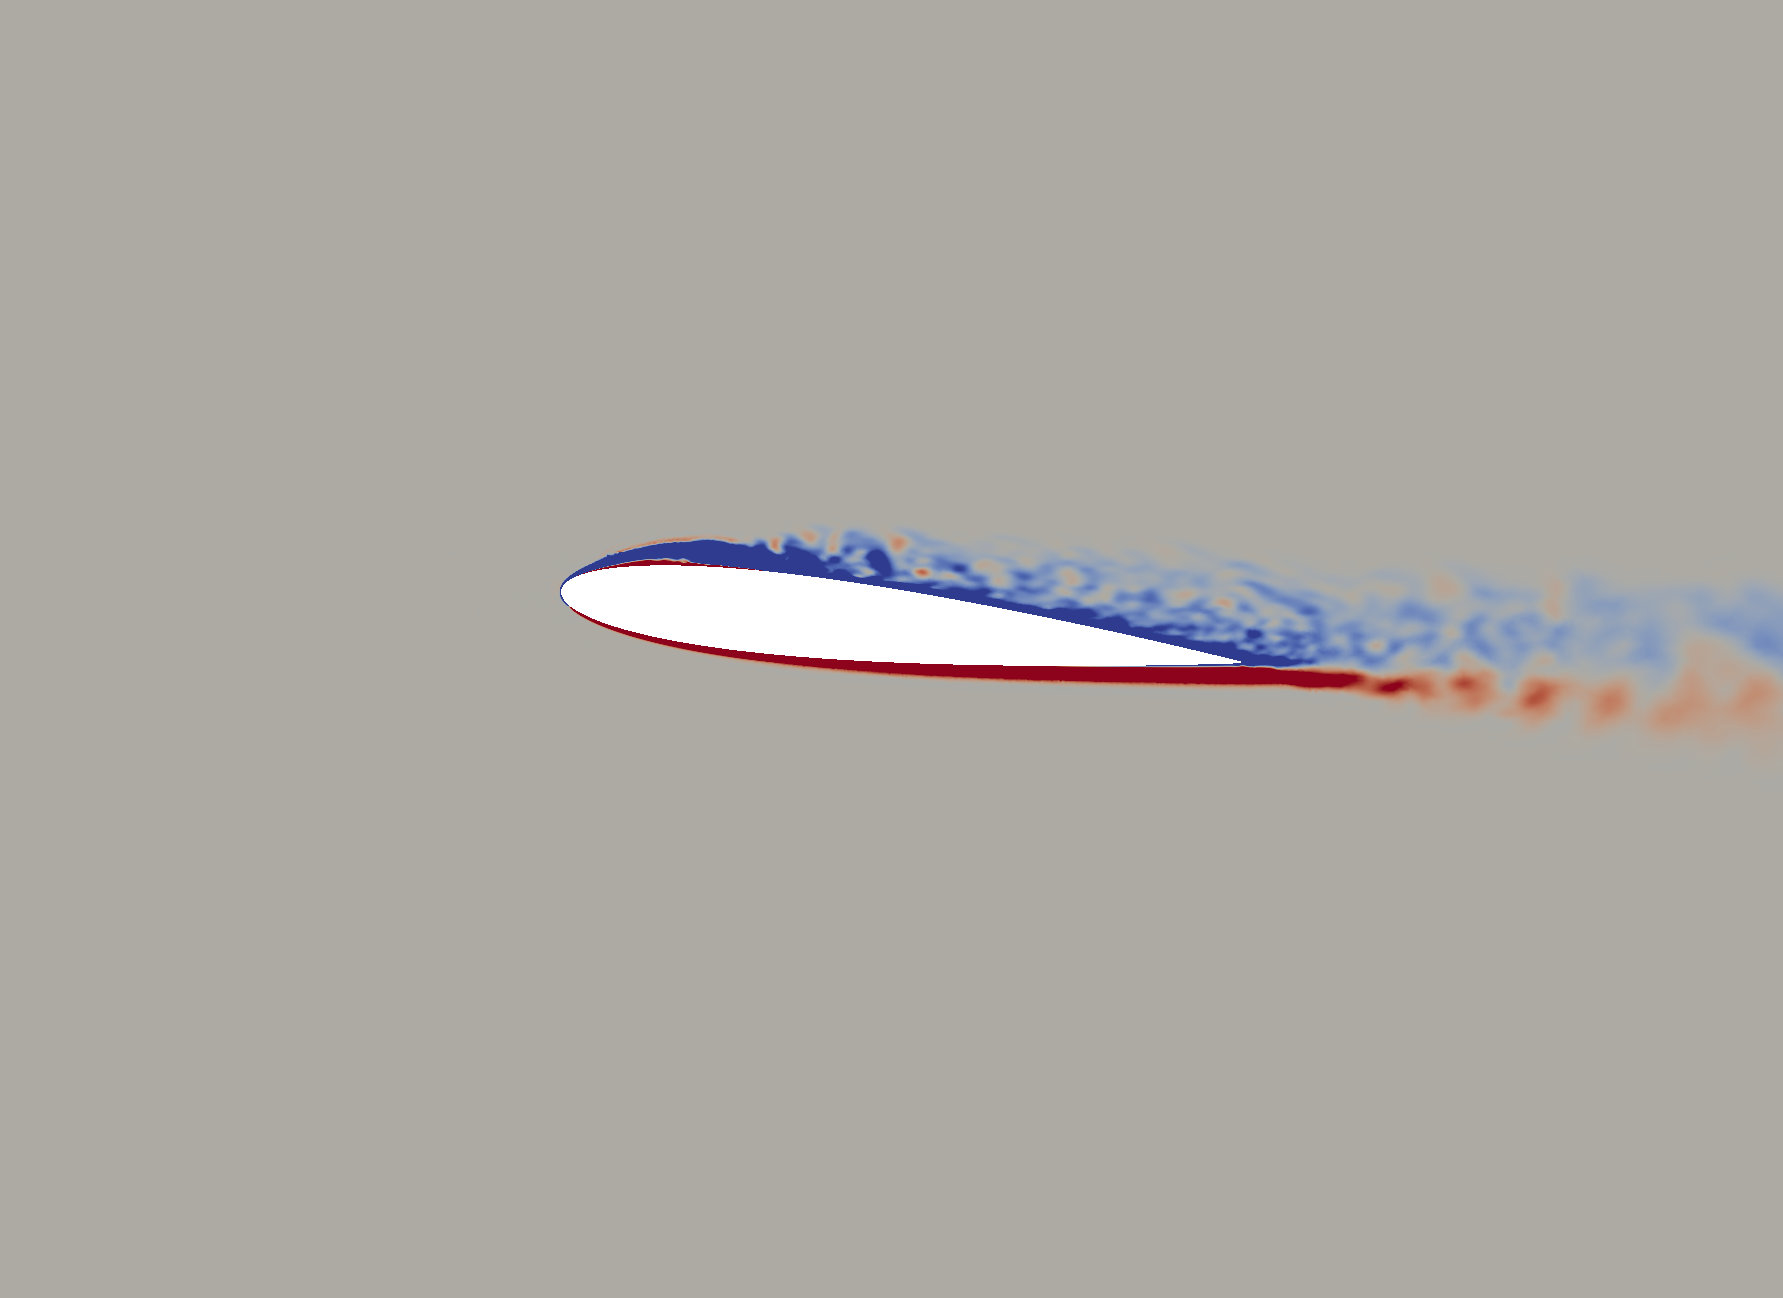
\includegraphics[width=1\textwidth]{figures/Vorticity_plots/Re_40k_1pt0/phase_195.png}
		\caption{$Re=4e4$, $\psi$ = $195^\circ$, $\tilde{t}=0.542$}
		\label{fig:Re_40k_1pt0_phi195}
	\end{subfigure}
	\begin{subfigure}[b]{0.32\textwidth}
		\centering
		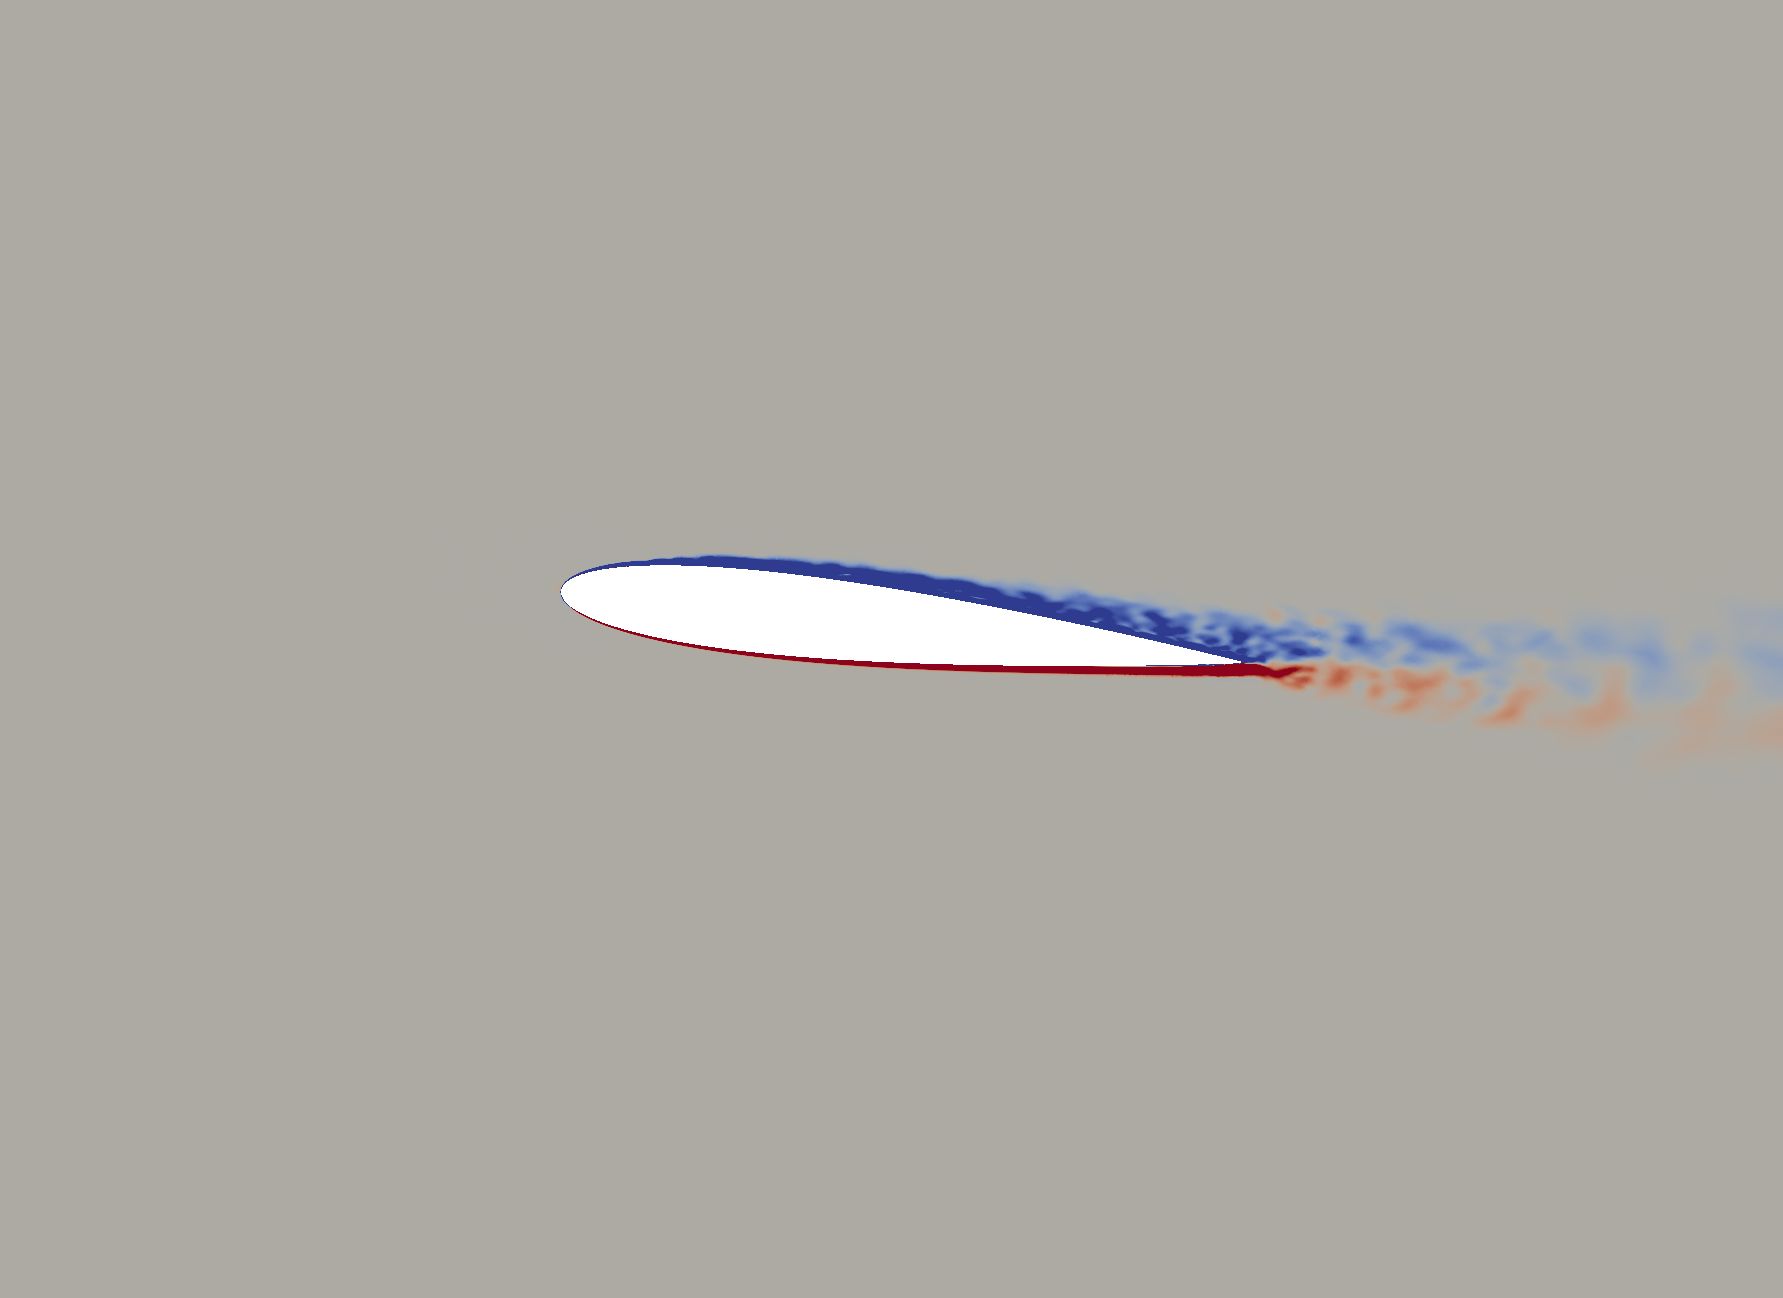
\includegraphics[width=1\textwidth]{figures/Vorticity_plots/Re_200k_1pt0/phase_195.png}
		\caption{$Re=2e5$, $\psi$ = $195^\circ$, $\tilde{t}=0.542$}
		\label{fig:Re_200k_1pt0_phi195}
	\end{subfigure}
	\begin{subfigure}[b]{0.32\textwidth}
		\centering
		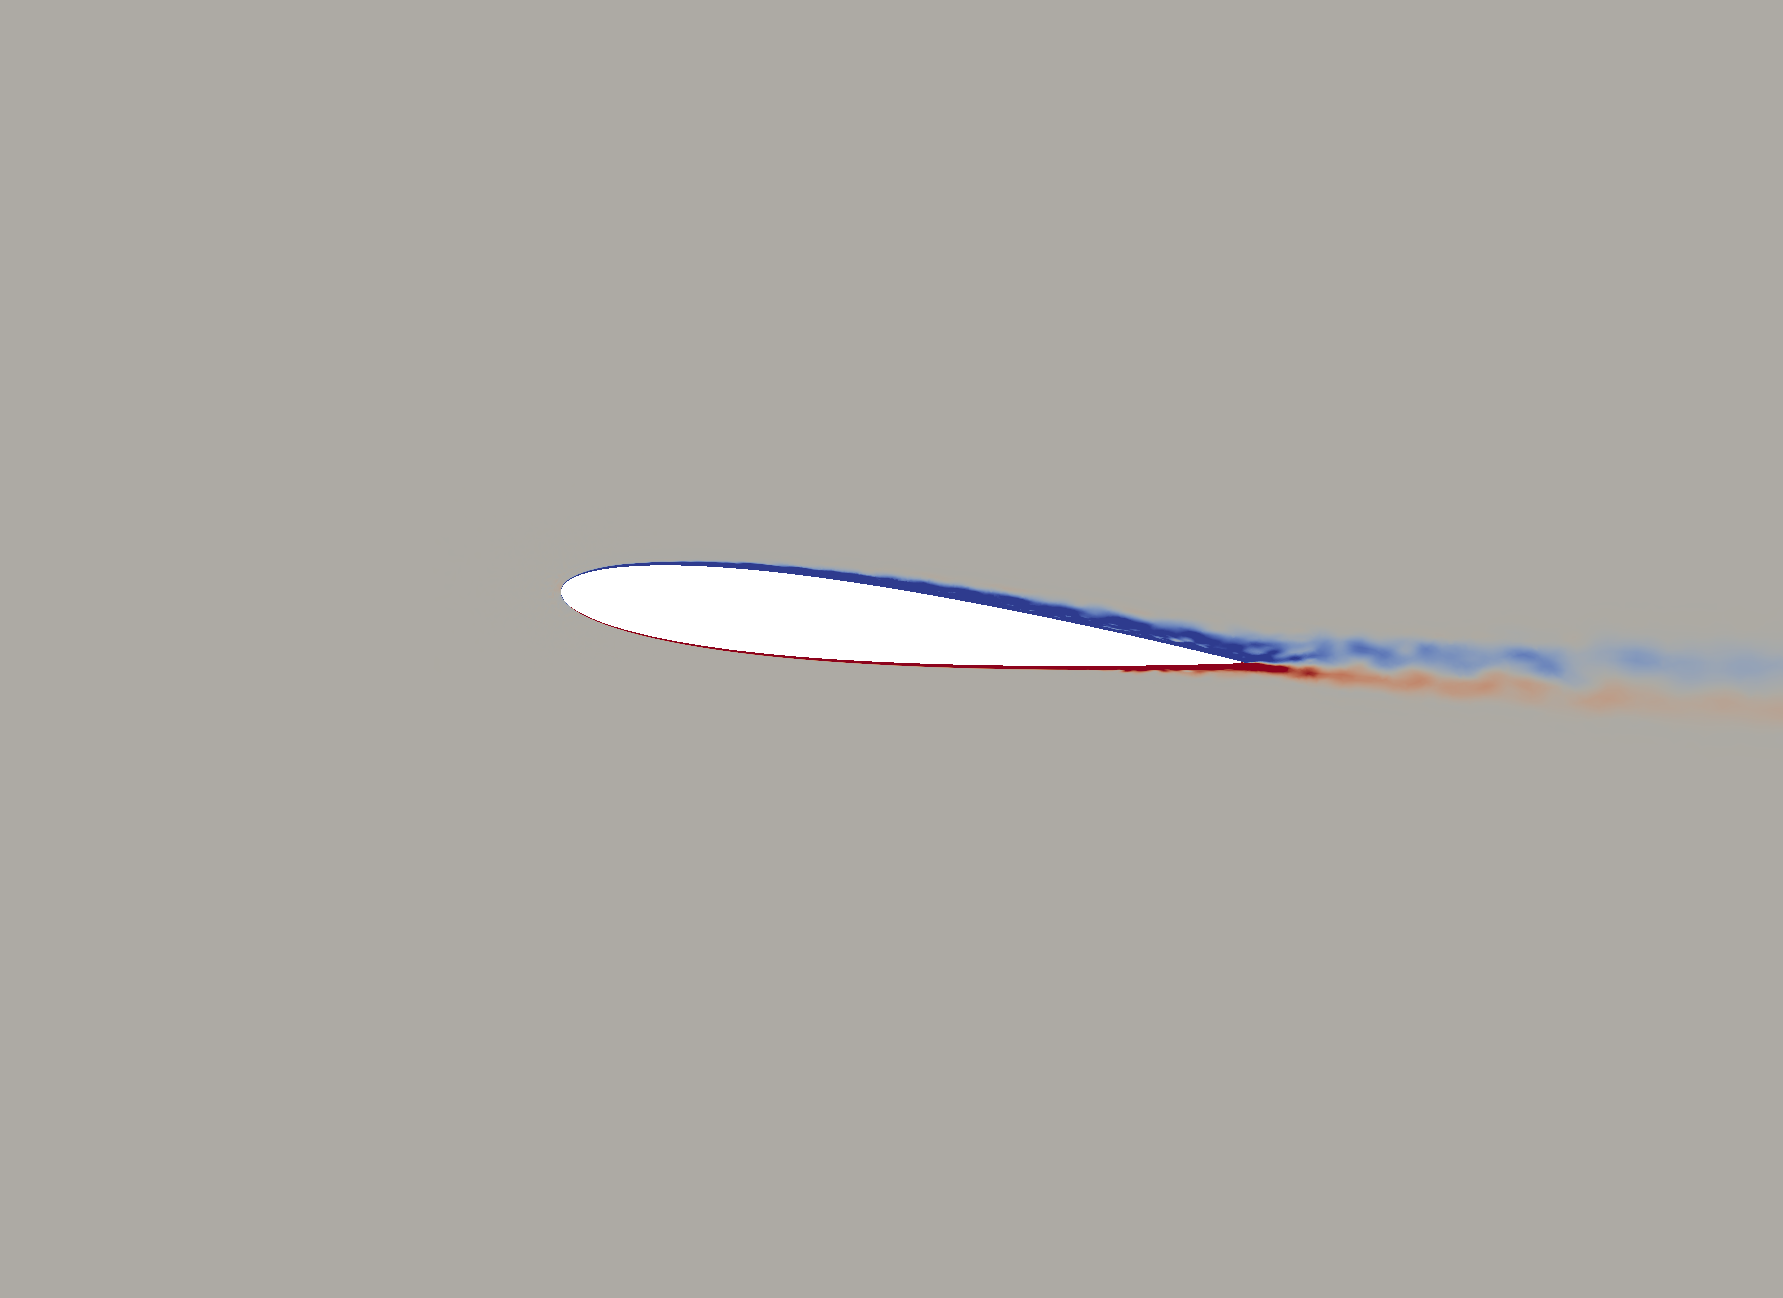
\includegraphics[width=1\textwidth]{figures/Vorticity_plots/Re_1m_1pt0/phase_195.png}
		\caption{$Re= 1e6$, $\psi$ = $195^\circ$, $\tilde{t}=0.542$}
		\label{fig:Re_1m_1pt0_phi195}
	\end{subfigure}
	
	\begin{subfigure}[b]{0.32\textwidth}
		\centering
		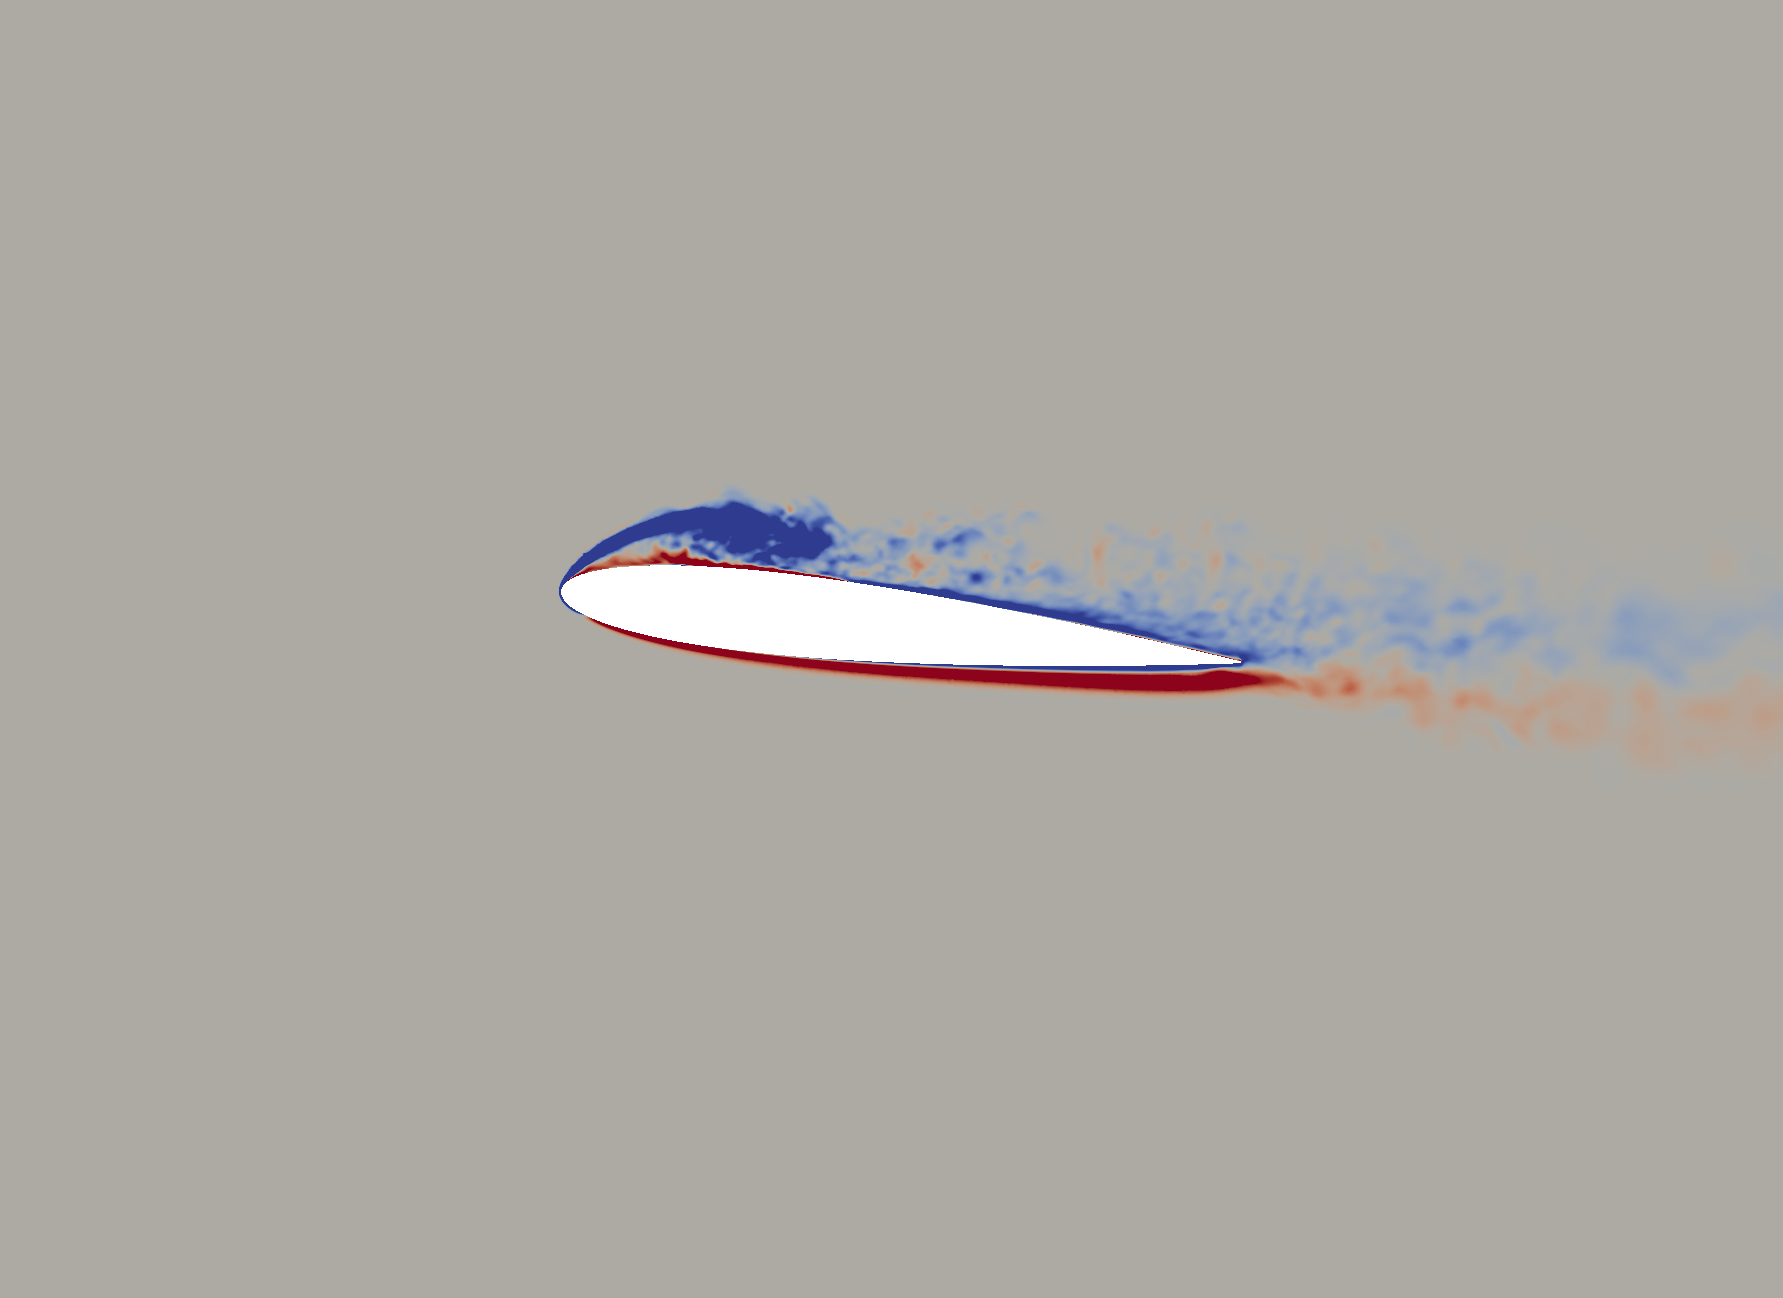
\includegraphics[width=1\textwidth]{figures/Vorticity_plots/Re_40k_1pt0/phase_225.png}
		\caption{$Re=4e4$, $\psi$ = $225^\circ$, $\tilde{t}=0.625$}
		\label{fig:Re_40k_1pt0_phi225}
	\end{subfigure}
	\begin{subfigure}[b]{0.32\textwidth}
		\centering
		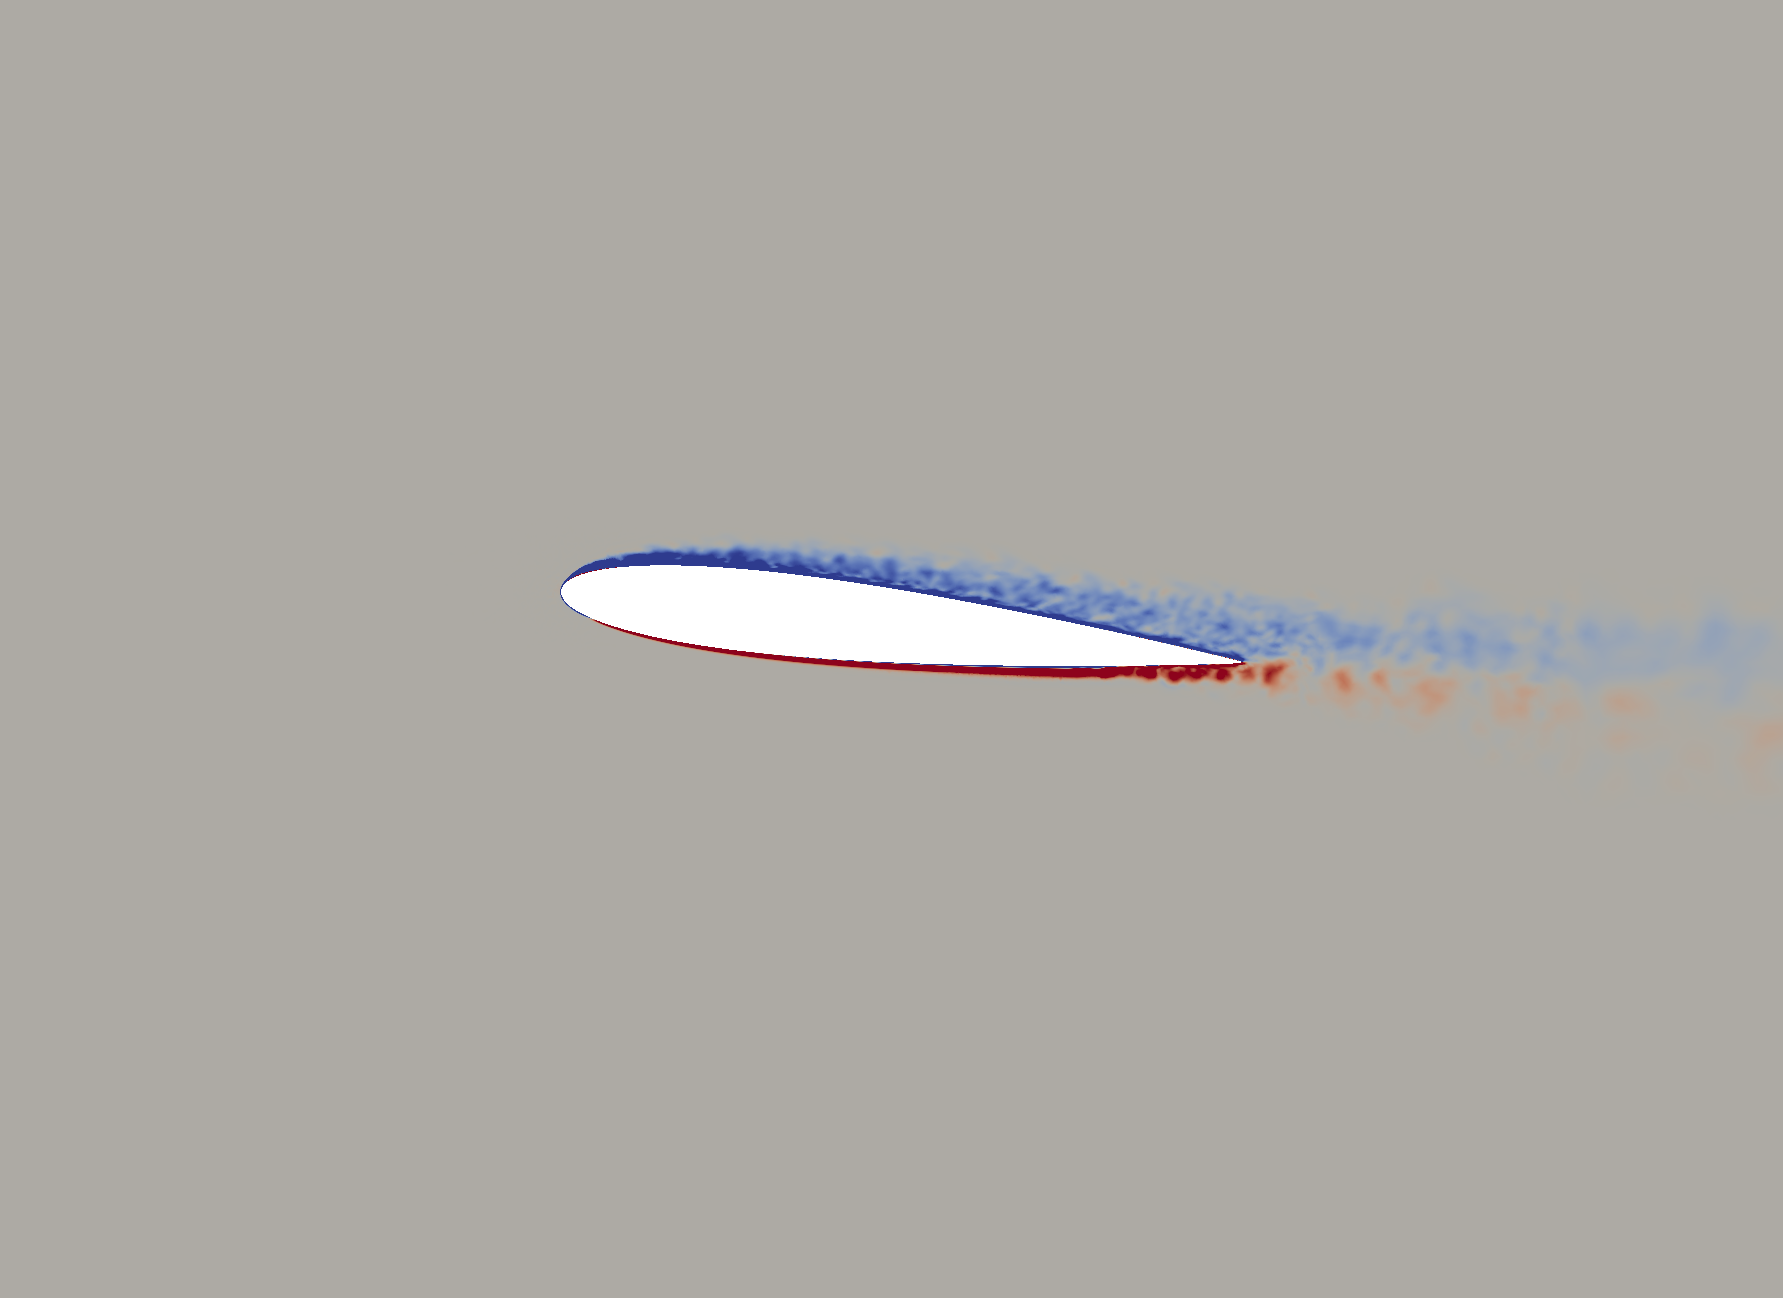
\includegraphics[width=1\textwidth]{figures/Vorticity_plots/Re_200k_1pt0/phase_225.png}
		\caption{$Re=2e5$, $\psi$ = $225^\circ$,  $\tilde{t}=0.625$}
		\label{fig:Re_200k_1pt0_phi225}
	\end{subfigure}
	\begin{subfigure}[b]{0.32\textwidth}
		\centering
		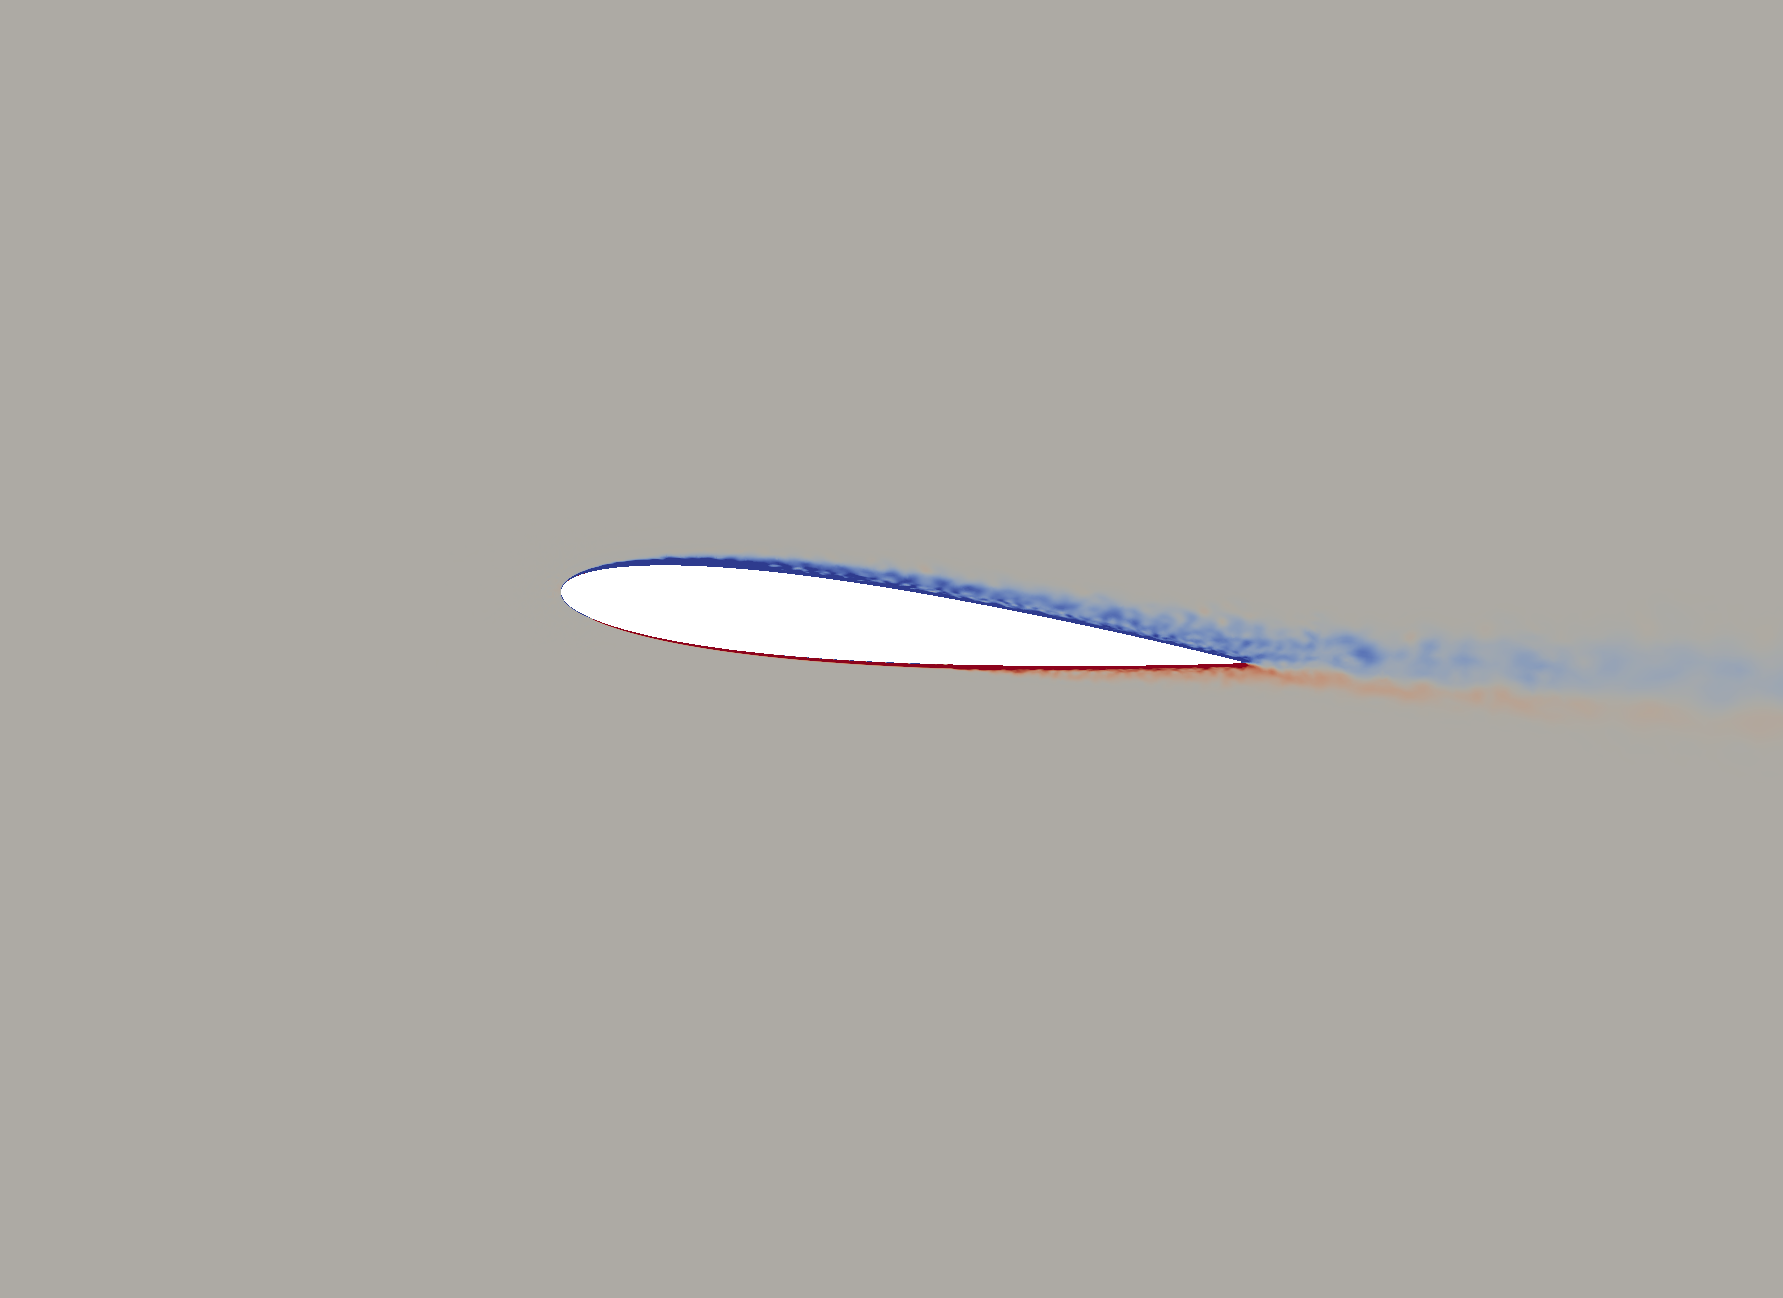
\includegraphics[width=1\textwidth]{figures/Vorticity_plots/Re_1m_1pt0/phase_225.png}
		\caption{$Re=1e6$, $\psi$ = $225^\circ$,  $\tilde{t}=0.625$}
		\label{fig:Re_1m_1pt0_phi225}
	\end{subfigure}
	
	\begin{subfigure}[b]{0.32\textwidth}
		\centering
		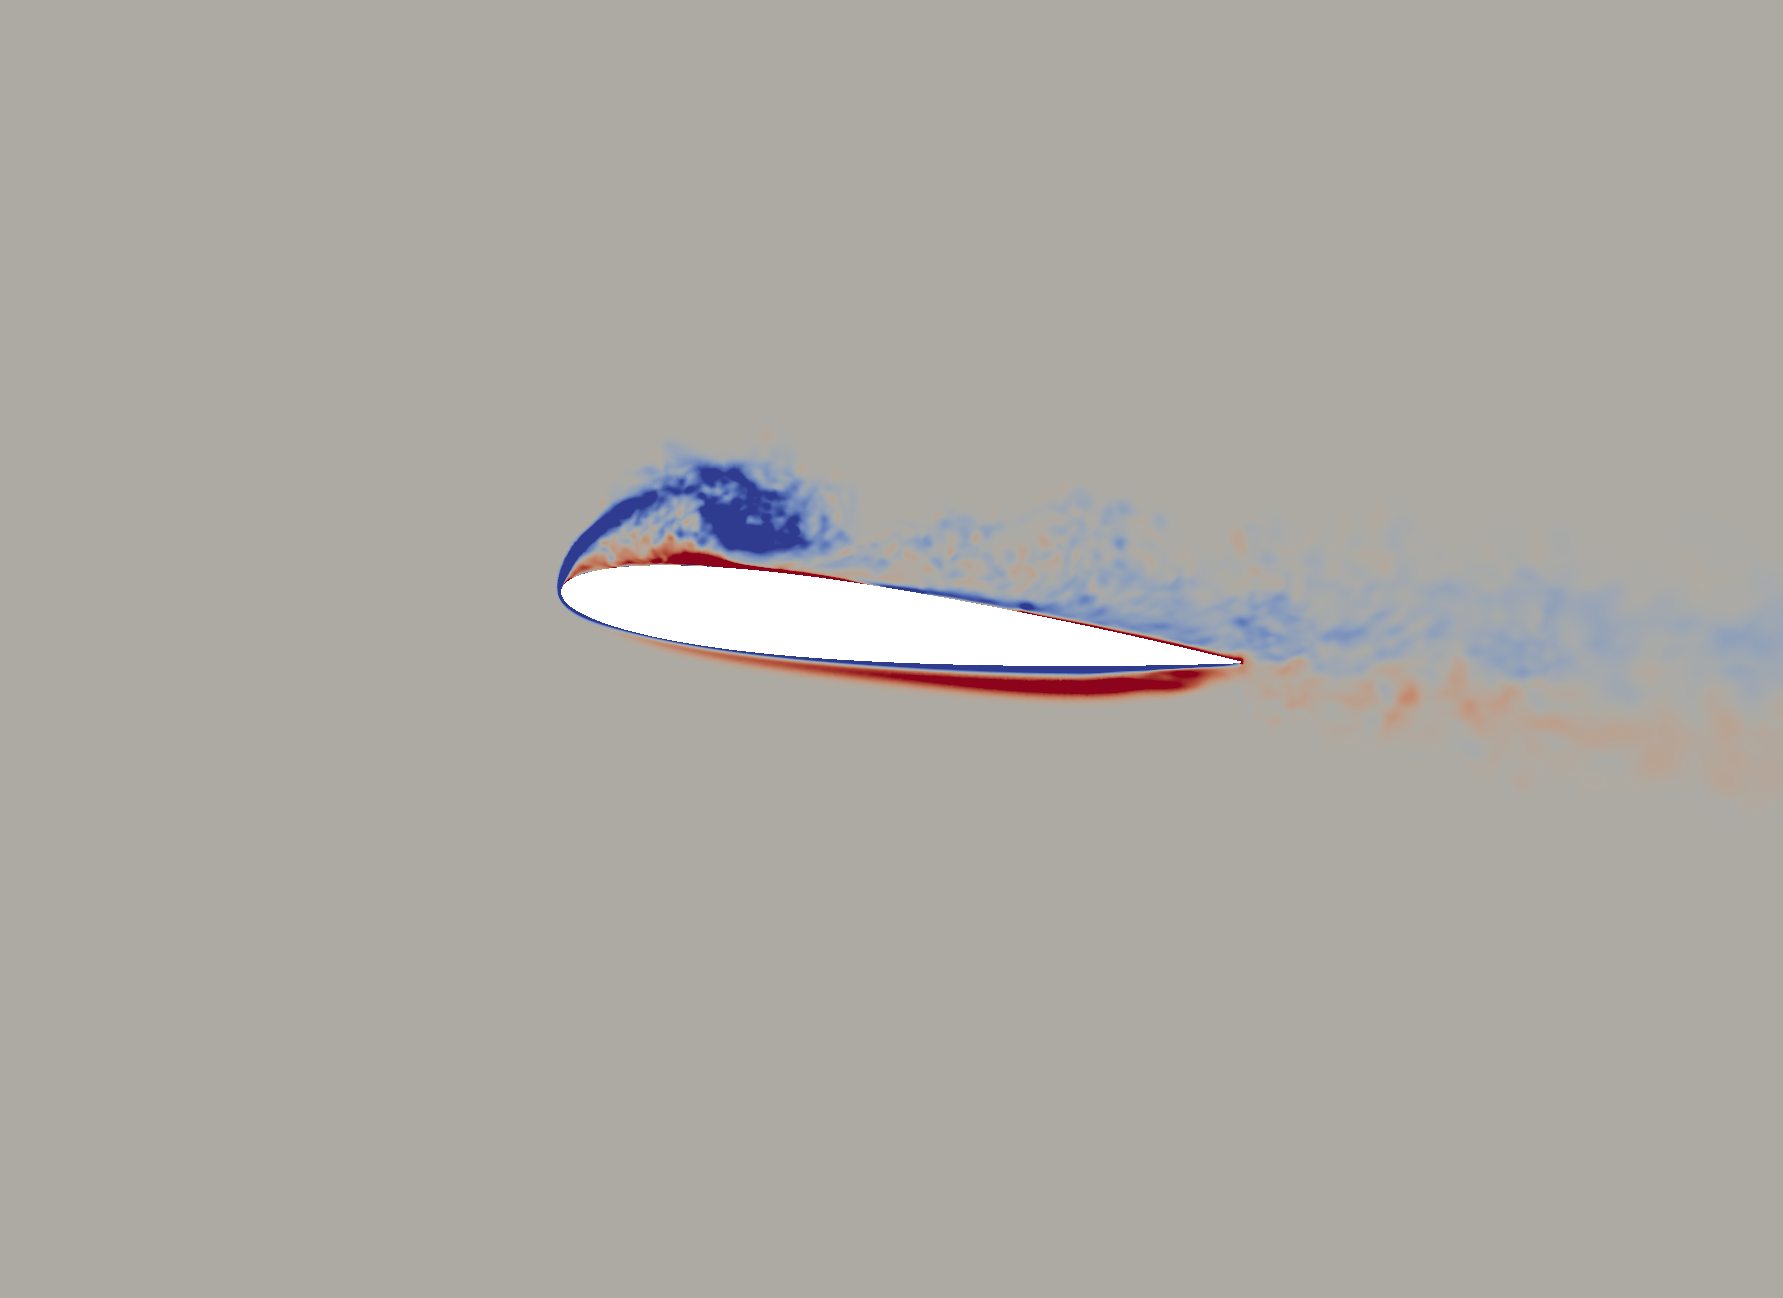
\includegraphics[width=1\textwidth]{figures/Vorticity_plots/Re_40k_1pt0/phase_240.png}
		\caption{$Re=4e4$, $\psi$ = $240^\circ$, $\tilde{t}=0.667$}
		\label{fig:Re_40k_1pt0_phi240}
	\end{subfigure}
	\begin{subfigure}[b]{0.32\textwidth}
		\centering
		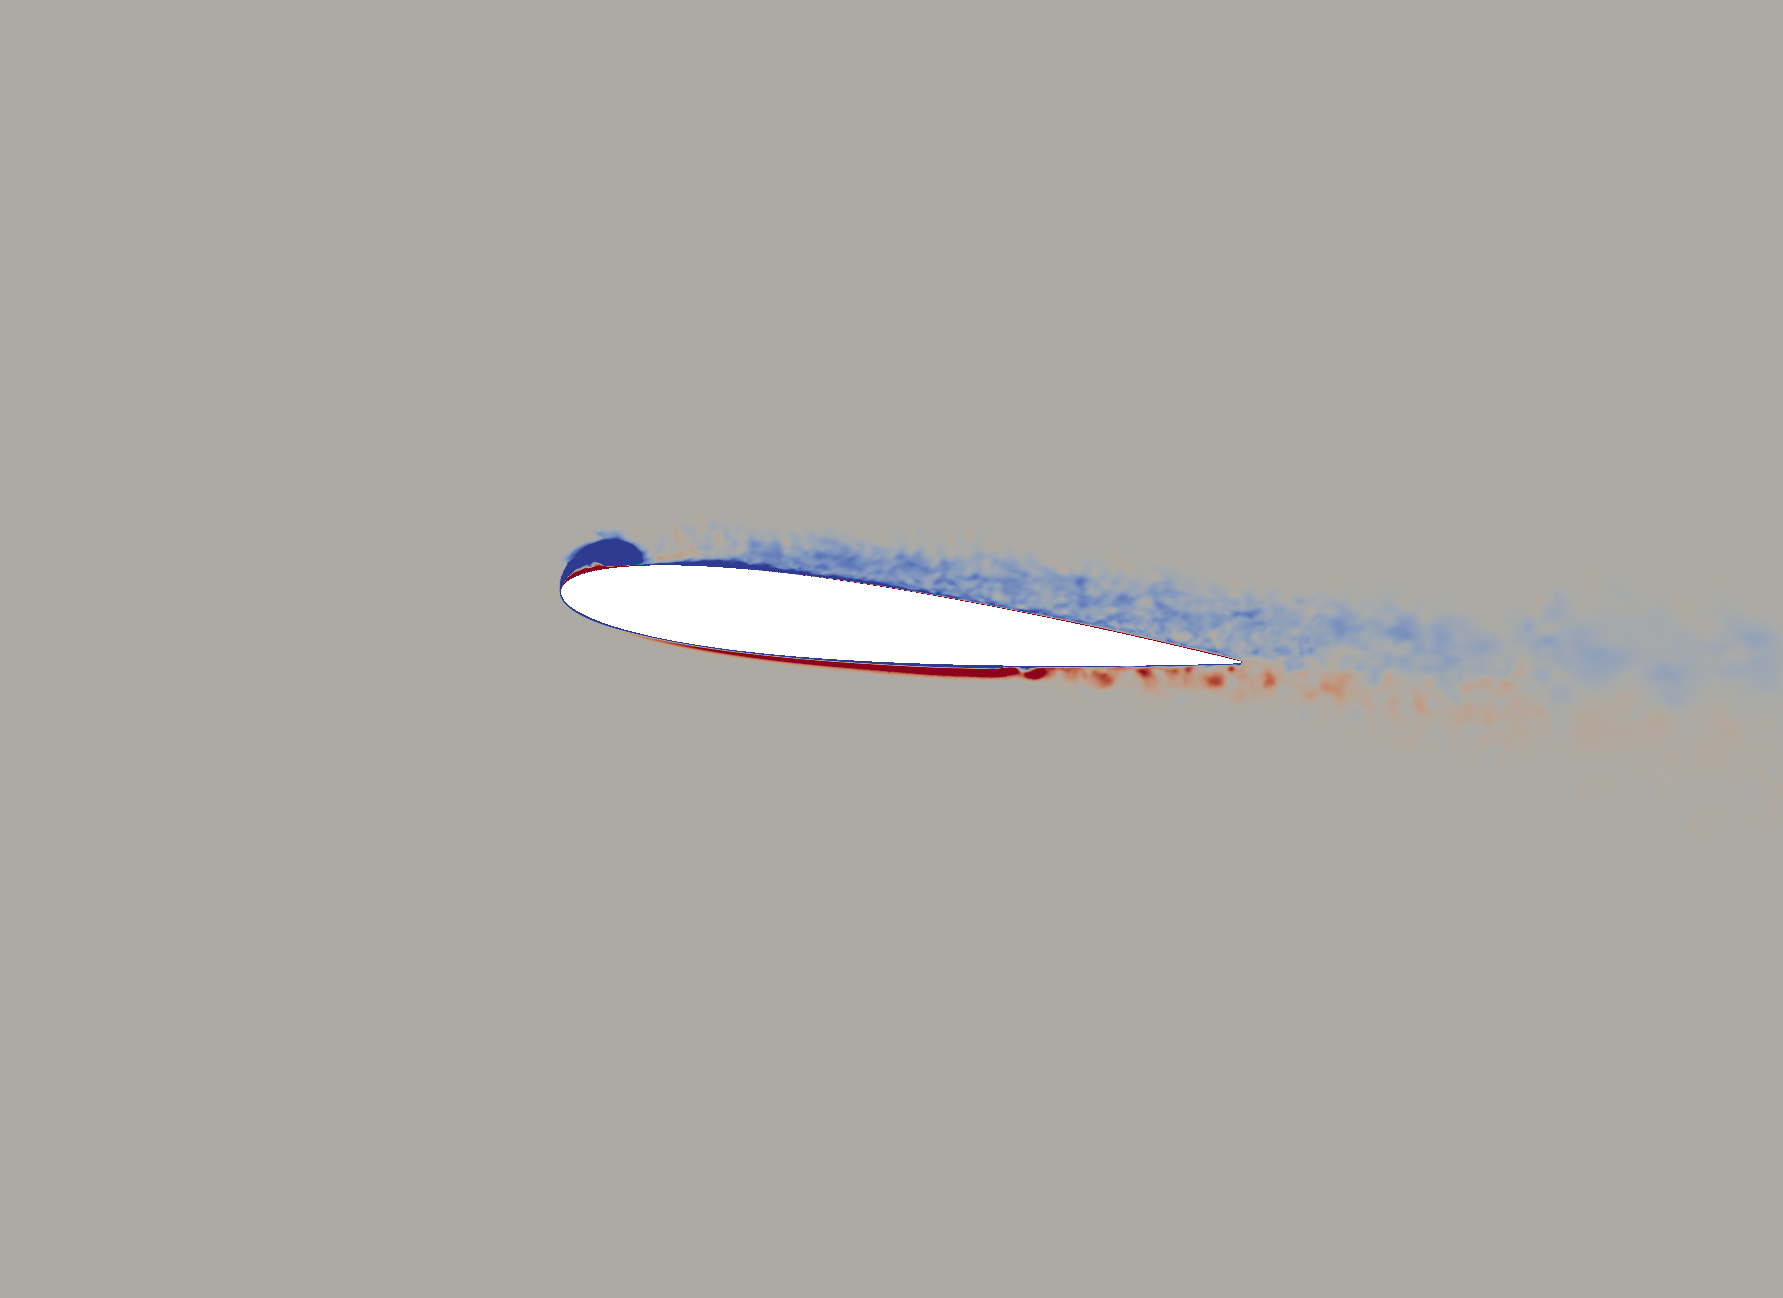
\includegraphics[width=1\textwidth]{figures/Vorticity_plots/Re_200k_1pt0/phase_240.png}
		\caption{$Re=2e5$, $\psi$ = $240^\circ$, $\tilde{t}=0.667$}
		\label{fig:Re_200k_1pt0_phi240}
	\end{subfigure}
	\begin{subfigure}[b]{0.32\textwidth}
		\centering
		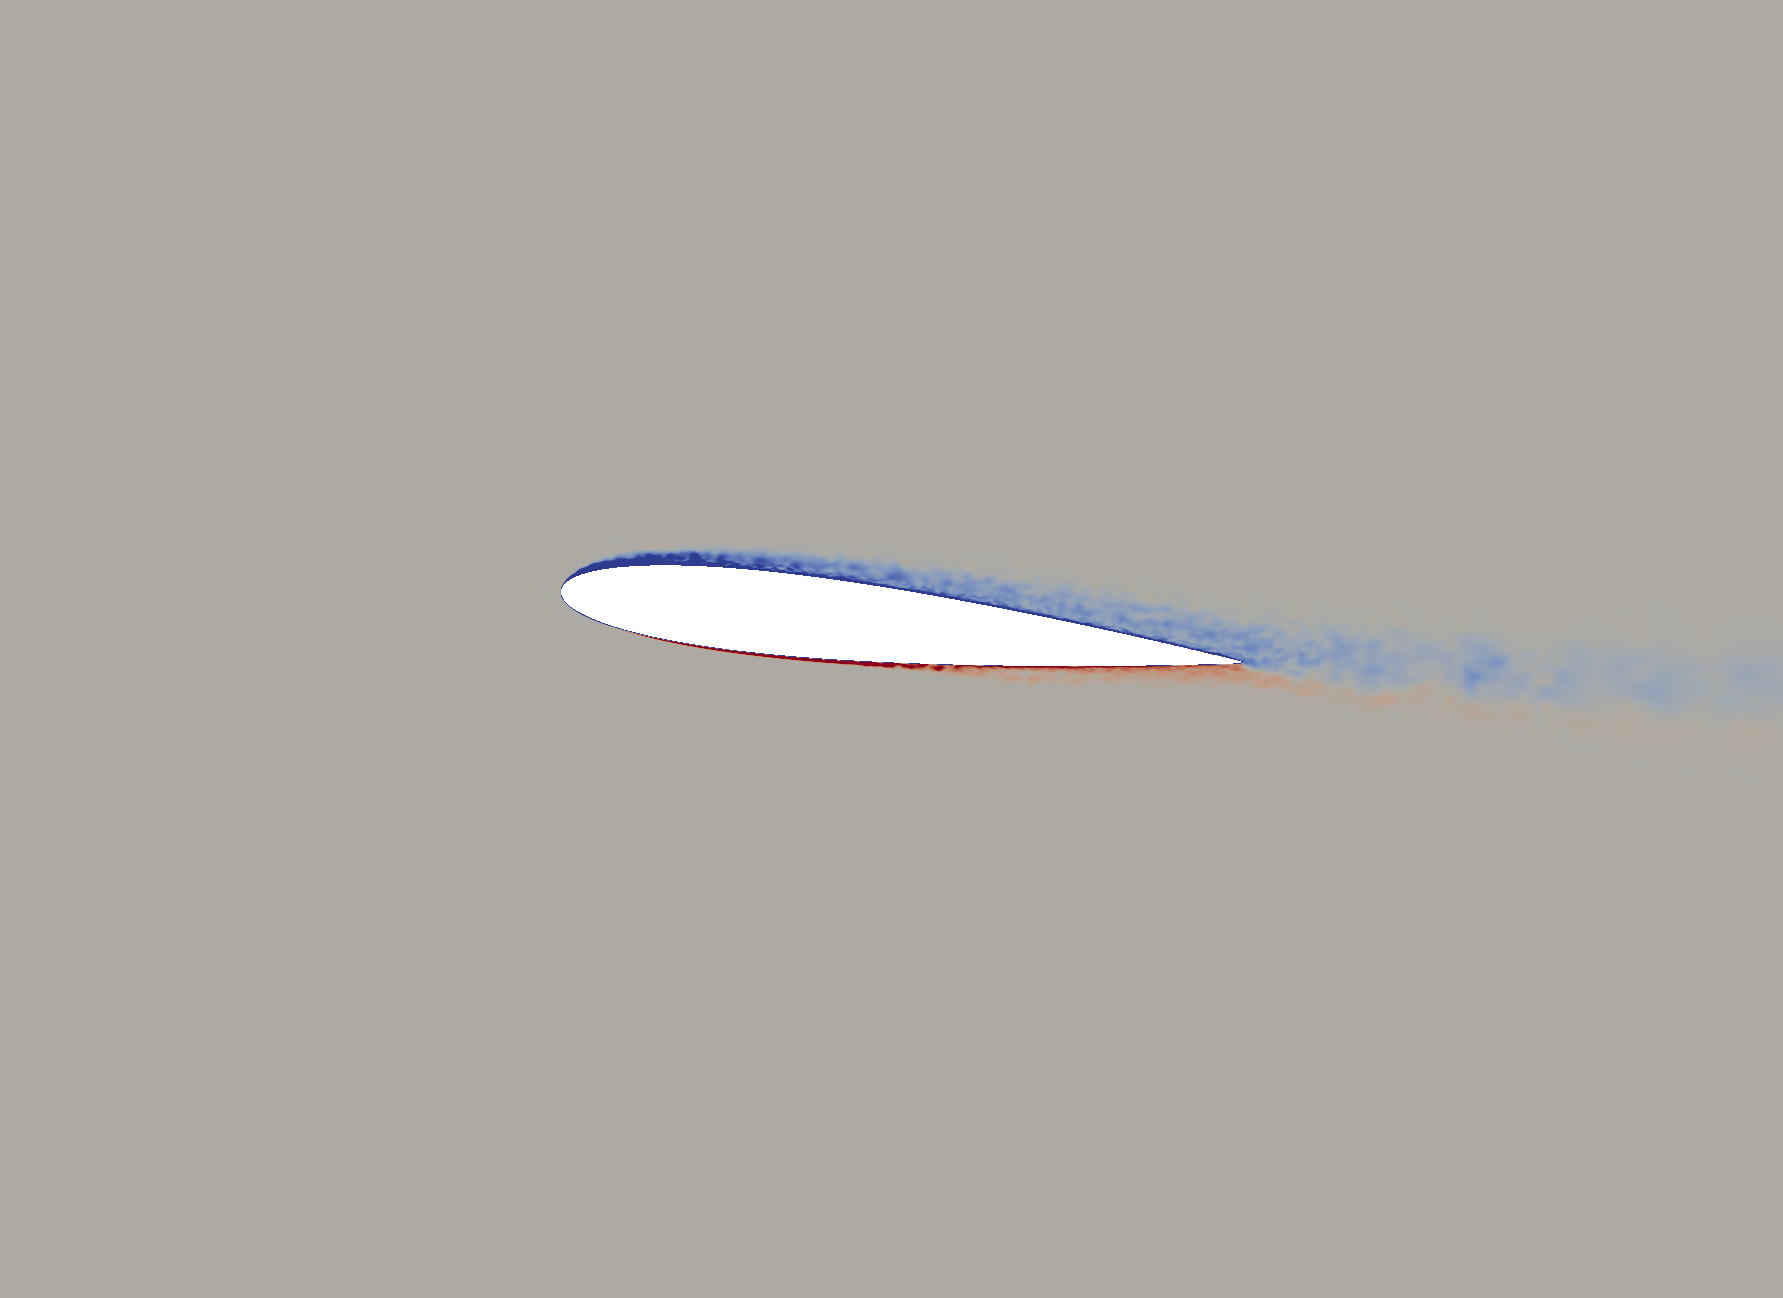
\includegraphics[width=1\textwidth]{figures/Vorticity_plots/Re_1m_1pt0/phase_240.png}
		\caption{$Re=1e6$, $\psi$ = $240^\circ$, $\tilde{t}=0.667$}
		\label{fig:Re_1m_1pt0_phi240}
	\end{subfigure}
	
	\begin{subfigure}[b]{0.32\textwidth}
		\centering
		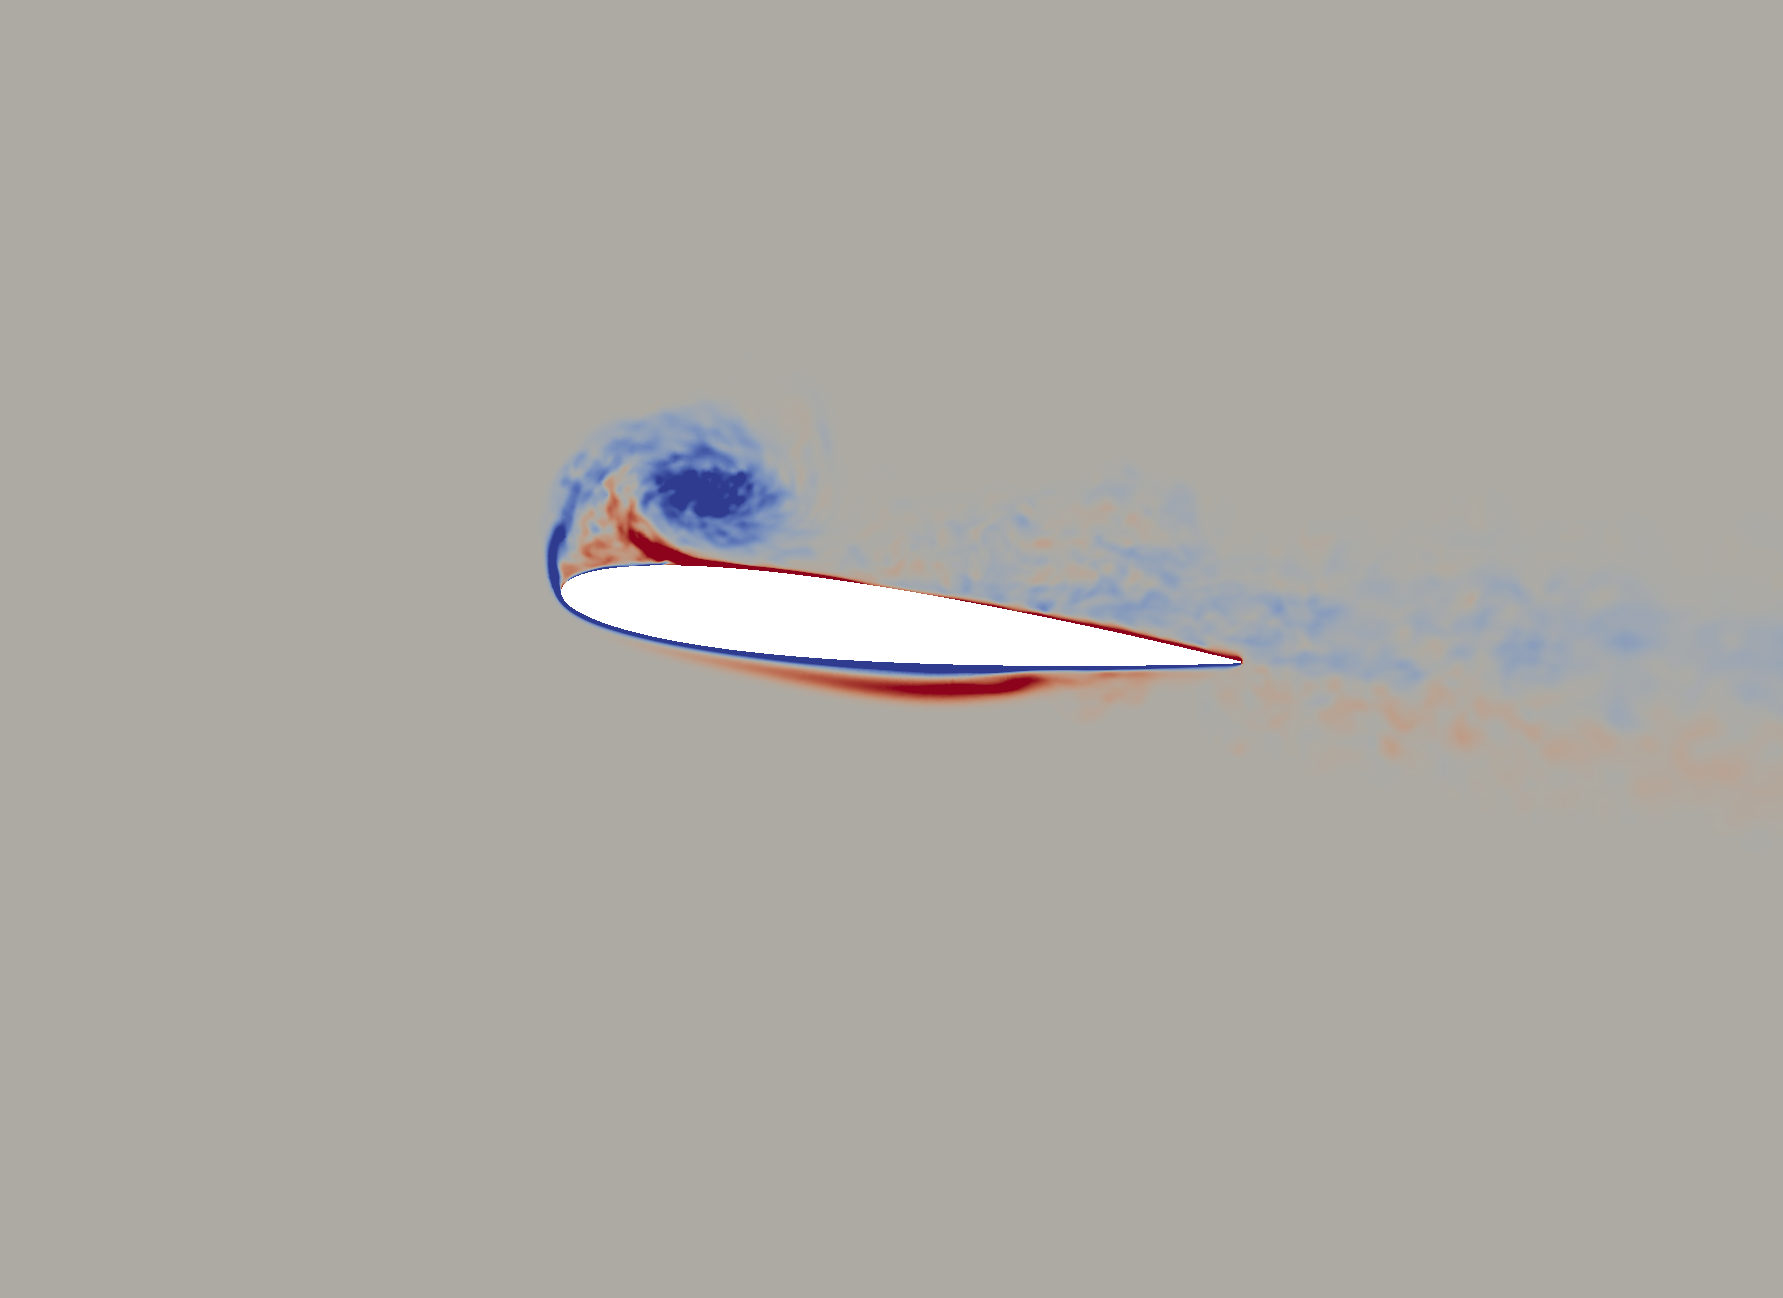
\includegraphics[width=1\textwidth]{figures/Vorticity_plots/Re_40k_1pt0/phase_255.png}
		\caption{$Re=4e4$, $\psi$ = $255^\circ$, $\tilde{t}=0.708$}
		\label{fig:Re_40k_1pt0_phi255}
	\end{subfigure}
	\begin{subfigure}[b]{0.32\textwidth}
		\centering
		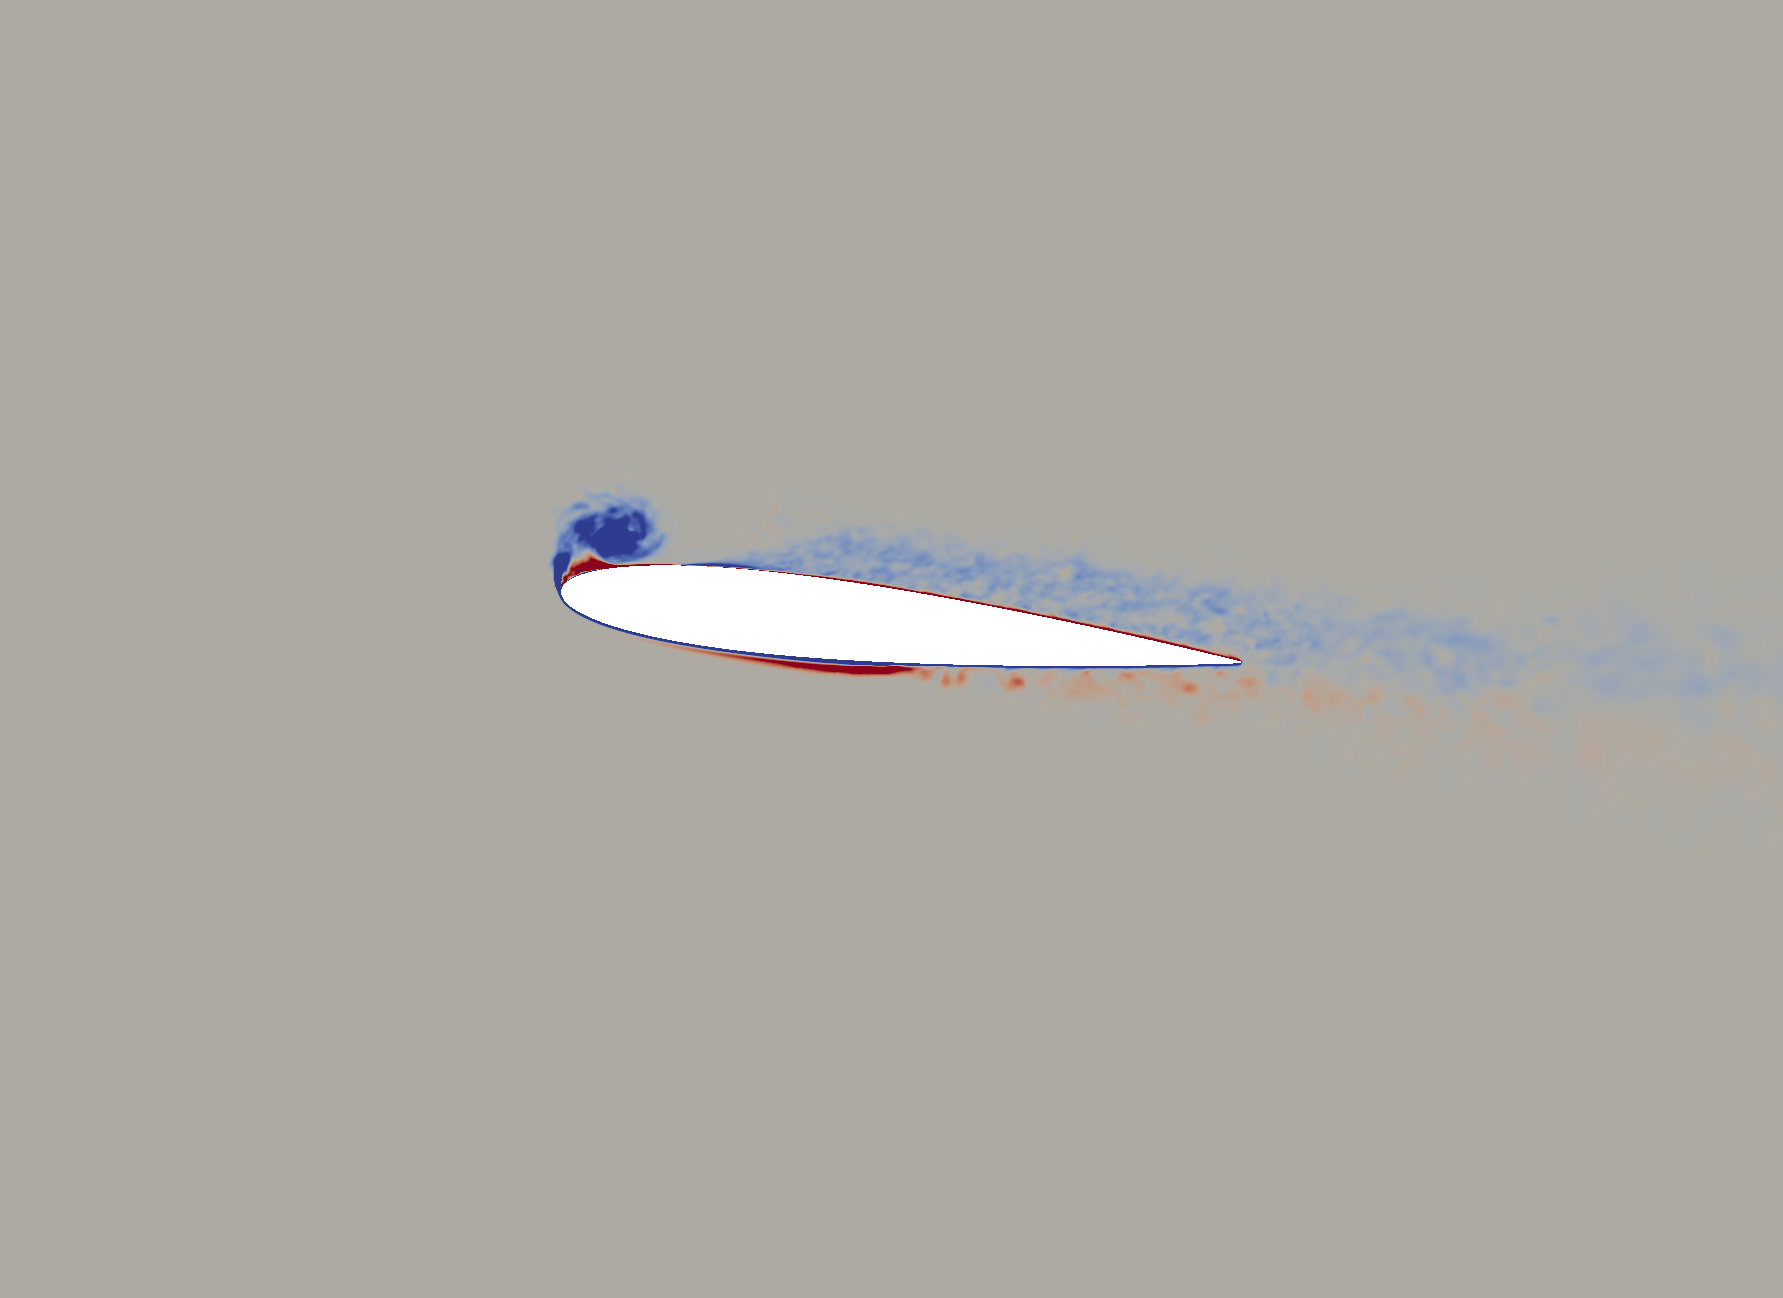
\includegraphics[width=1\textwidth]{figures/Vorticity_plots/Re_200k_1pt0/phase_255.png}
		\caption{$Re=2e5$, $\psi$ = $255^\circ$, $\tilde{t}=0.708$}
		\label{fig:Re_200k_1pt0_phi255}
	\end{subfigure}
	\begin{subfigure}[b]{0.32\textwidth}
		\centering
		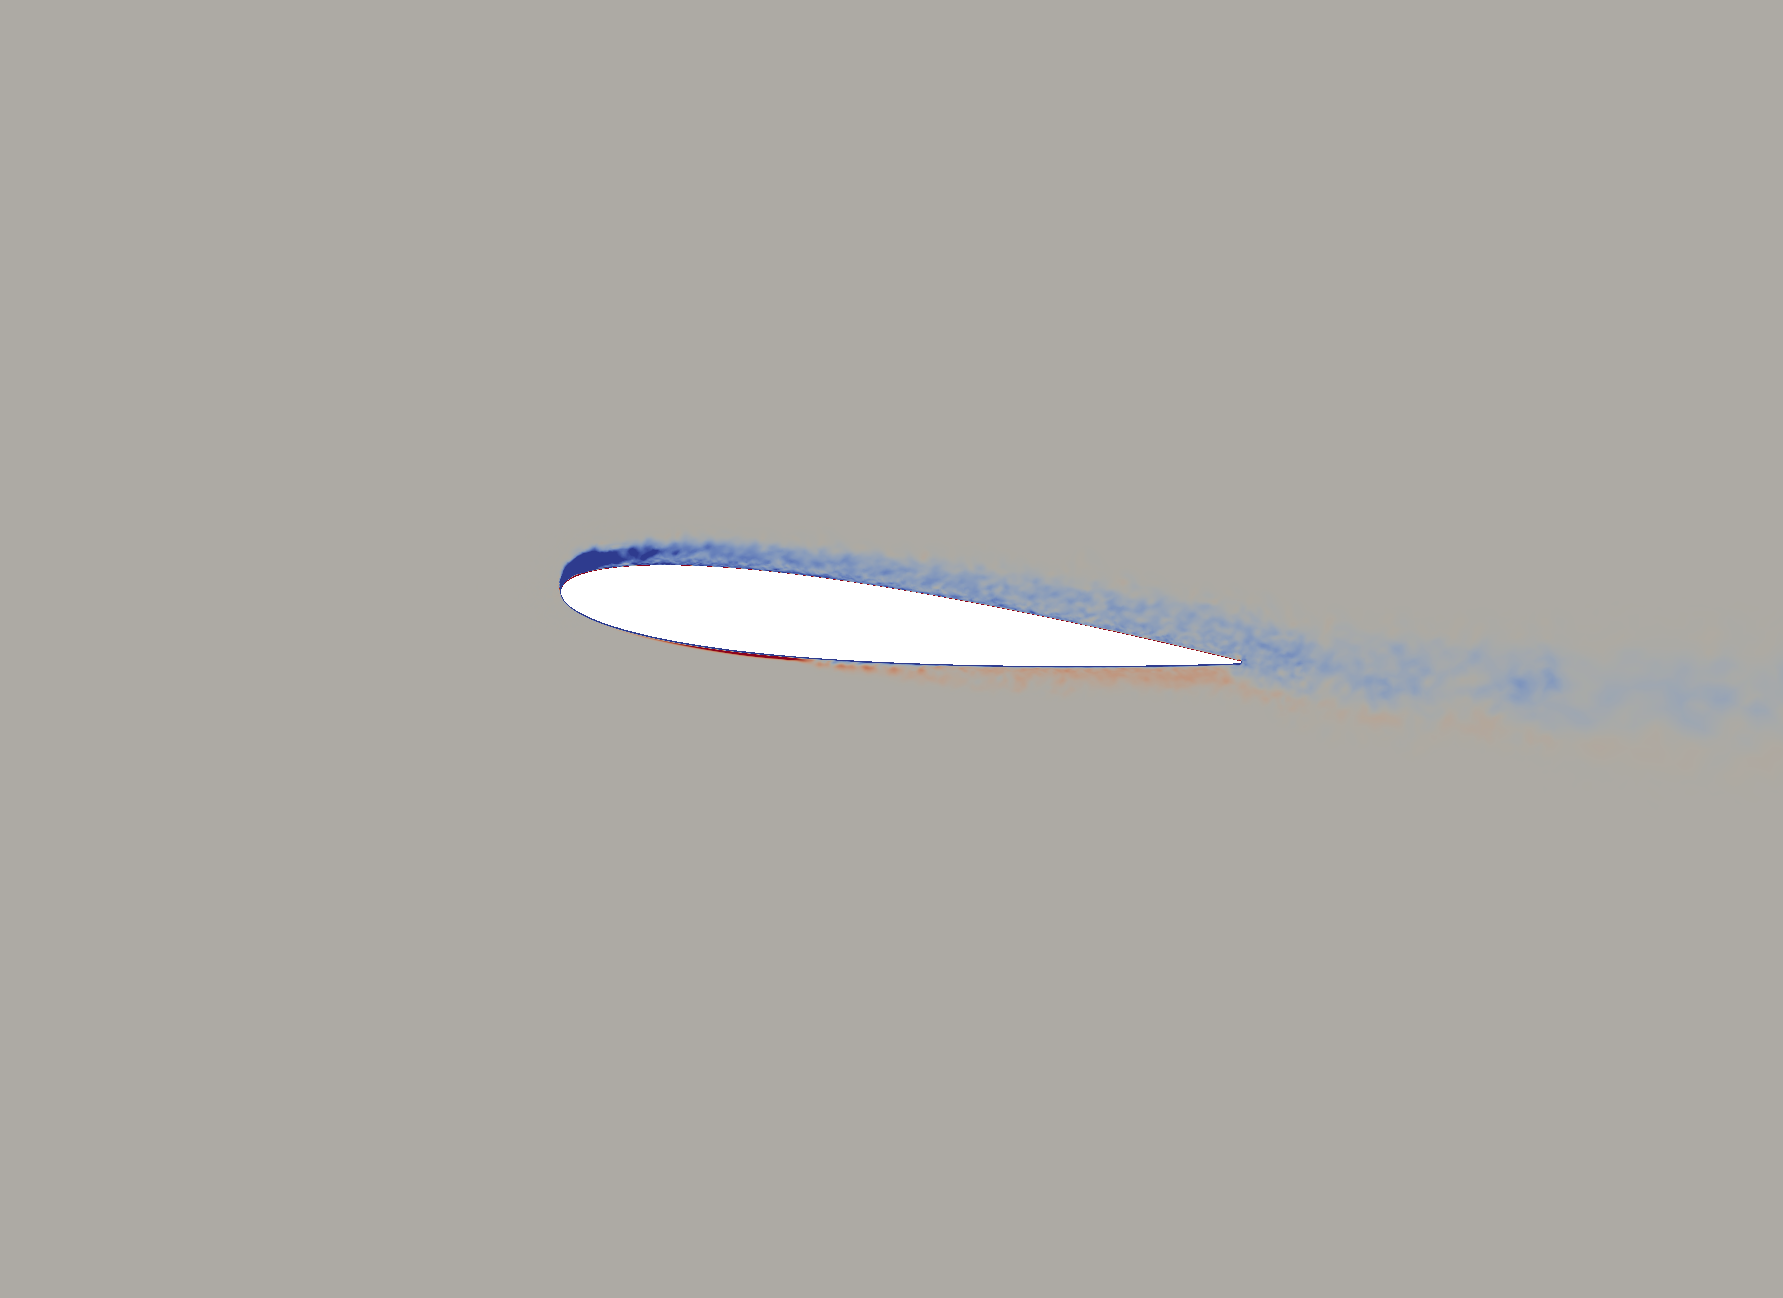
\includegraphics[width=1\textwidth]{figures/Vorticity_plots/Re_1m_1pt0/phase_255.png}
		\caption{$Re=1e6$, $\psi$ = $255^\circ$, $\tilde{t}=0.708$}
		\label{fig:Re_1m_1pt0_phi255}
	\end{subfigure}
	
	\caption{Spanwise vorticity at 8 different phases for $Re$=40,000 (left column), 200,000 (middle column) and 1,000,000 (right column) at $\mu_{sect}$ = 1.0}
	\label{fig:vortScreen_1pt0}
\end{figure}


\begin{figure}[H]\ContinuedFloat
	\centering
	\begin{subfigure}[b]{0.32\textwidth}
		\centering
		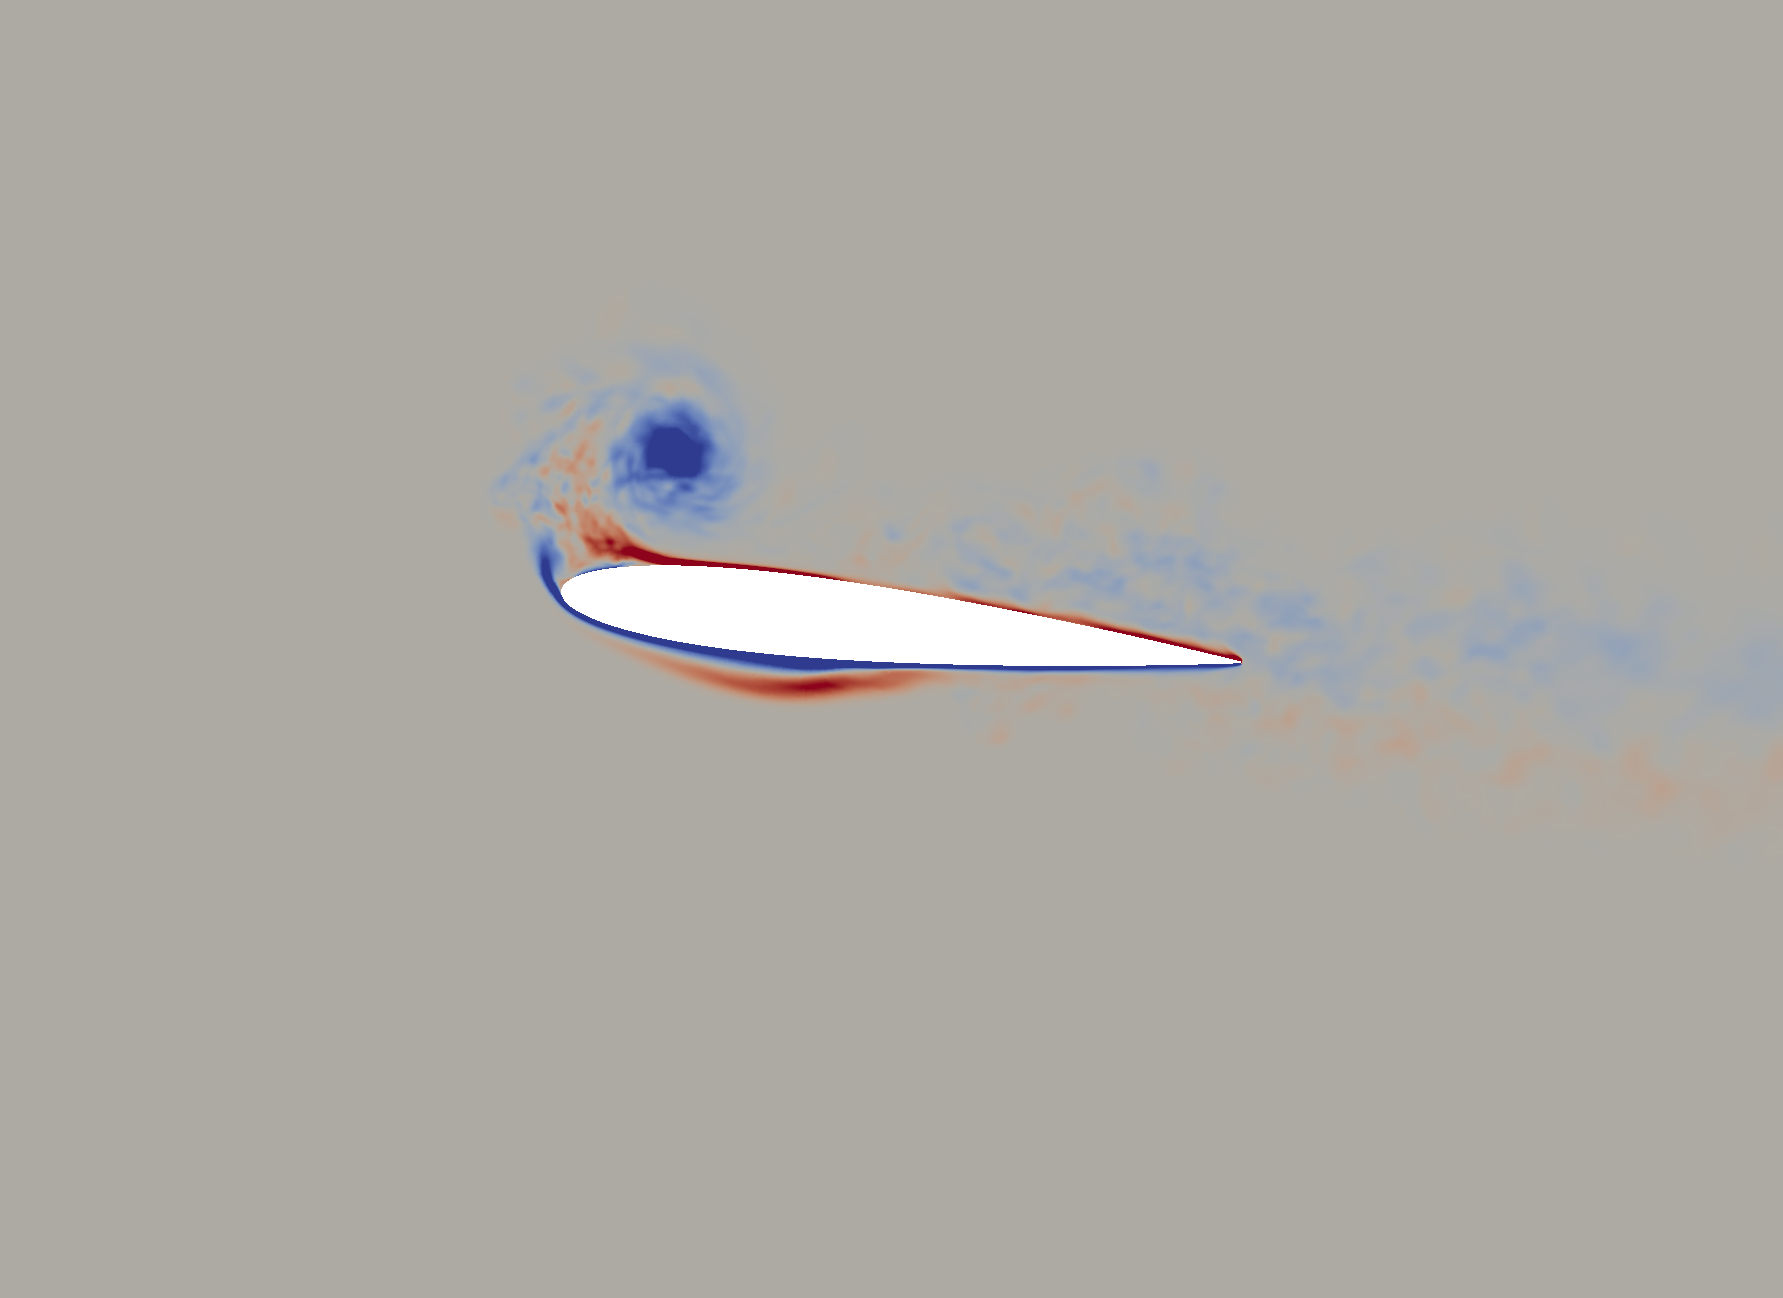
\includegraphics[width=1\textwidth]{figures/Vorticity_plots/Re_40k_1pt0/phase_270.png}
		\caption{$Re=4e4$, $\psi$ = $270^\circ$, $\tilde{t}=0.750$}
		\label{fig:Re_40k_1pt0_phi270}
	\end{subfigure}
	\begin{subfigure}[b]{0.32\textwidth}
		\centering
		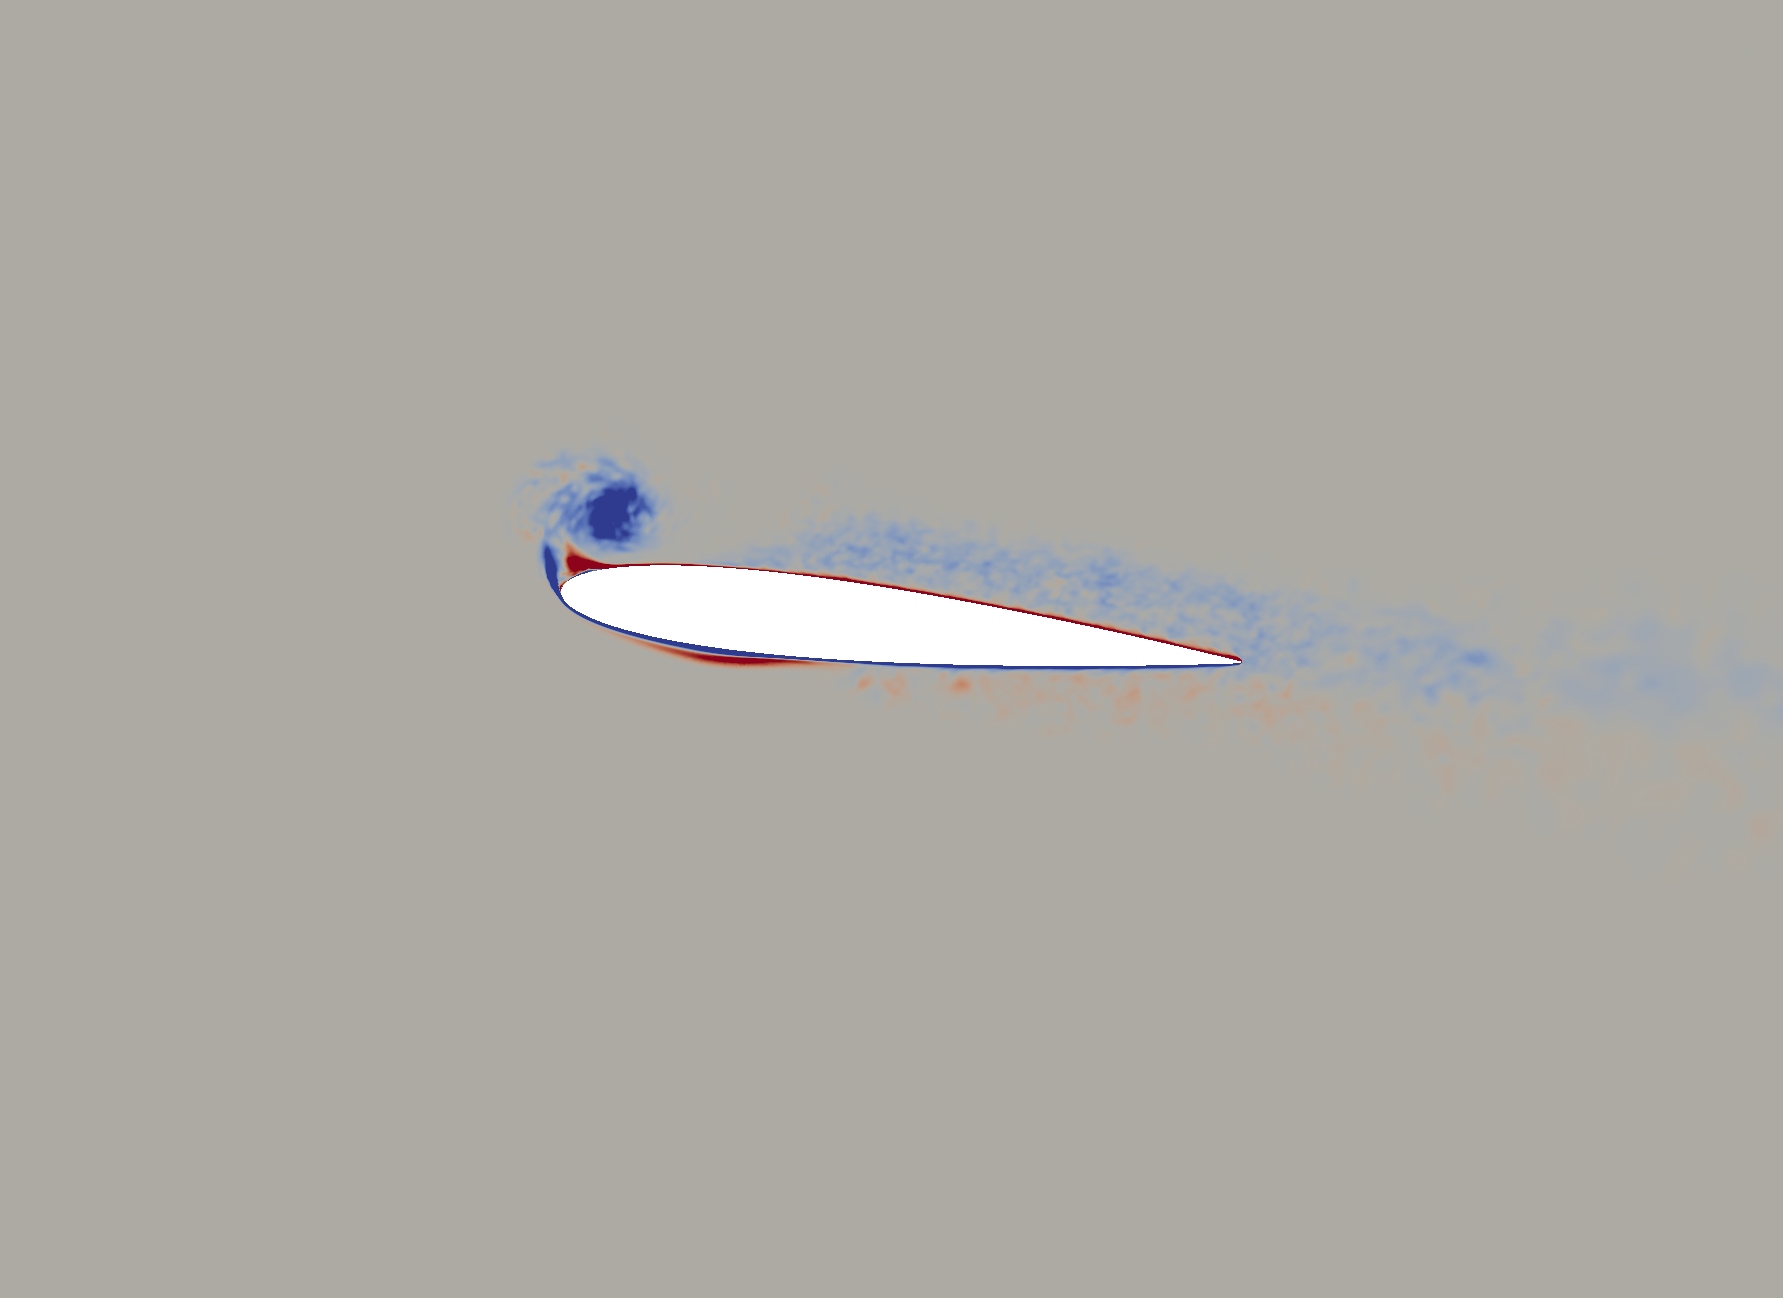
\includegraphics[width=1\textwidth]{figures/Vorticity_plots/Re_200k_1pt0/phase_270.png}
		\caption{$Re=2e5$, $\psi$ = $270^\circ$, $\tilde{t}=0.750$}
		\label{fig:Re_200k_1pt0_phi270}
	\end{subfigure}
	\begin{subfigure}[b]{0.32\textwidth}
		\centering
		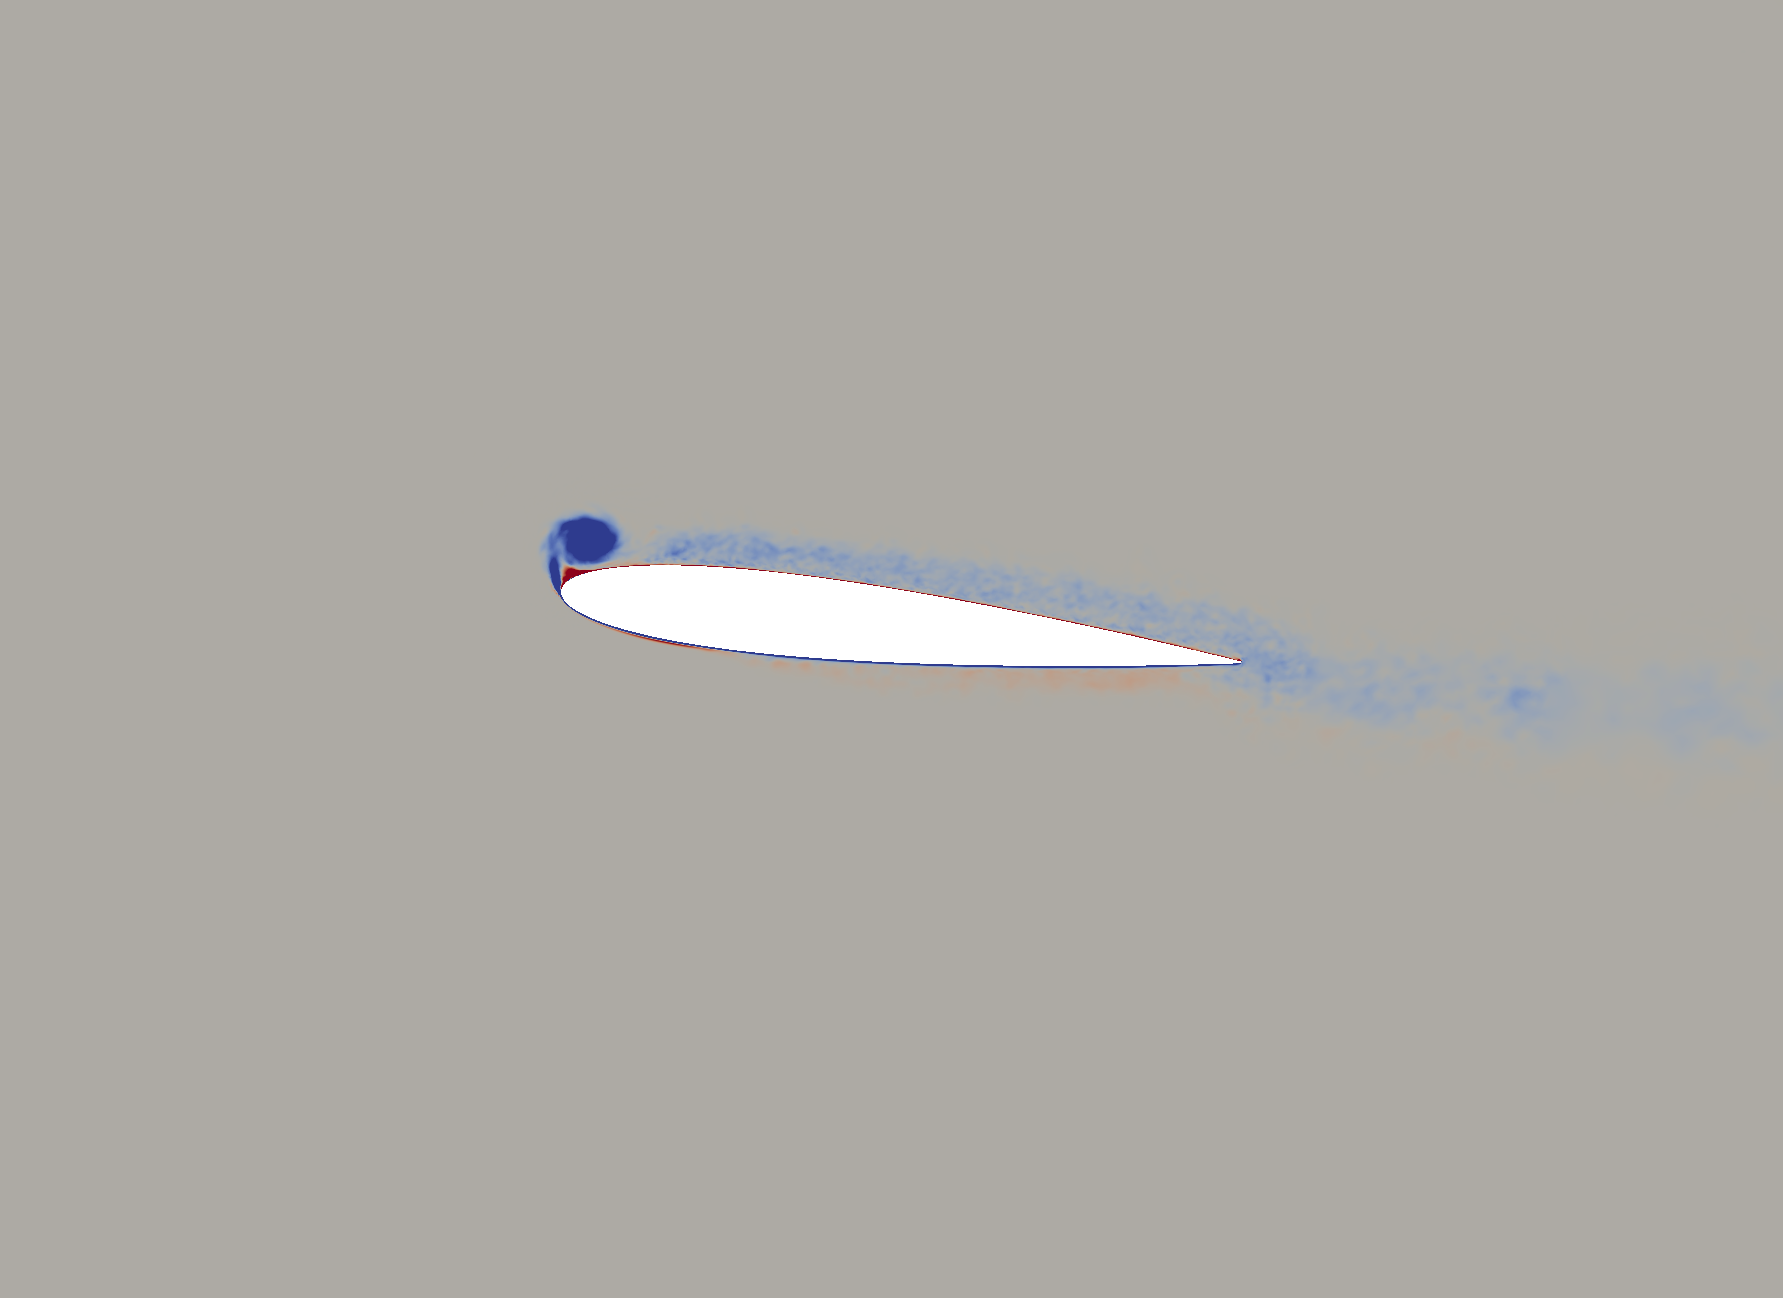
\includegraphics[width=1\textwidth]{figures/Vorticity_plots/Re_1m_1pt0/phase_270.png}
		\caption{$Re=1e6$, $\psi$ = $270^\circ$, $\tilde{t}=0.750$}
		\label{fig:Re_1m_1pt0_phi270}
	\end{subfigure}
	
	\begin{subfigure}[b]{0.32\textwidth}
		\centering
		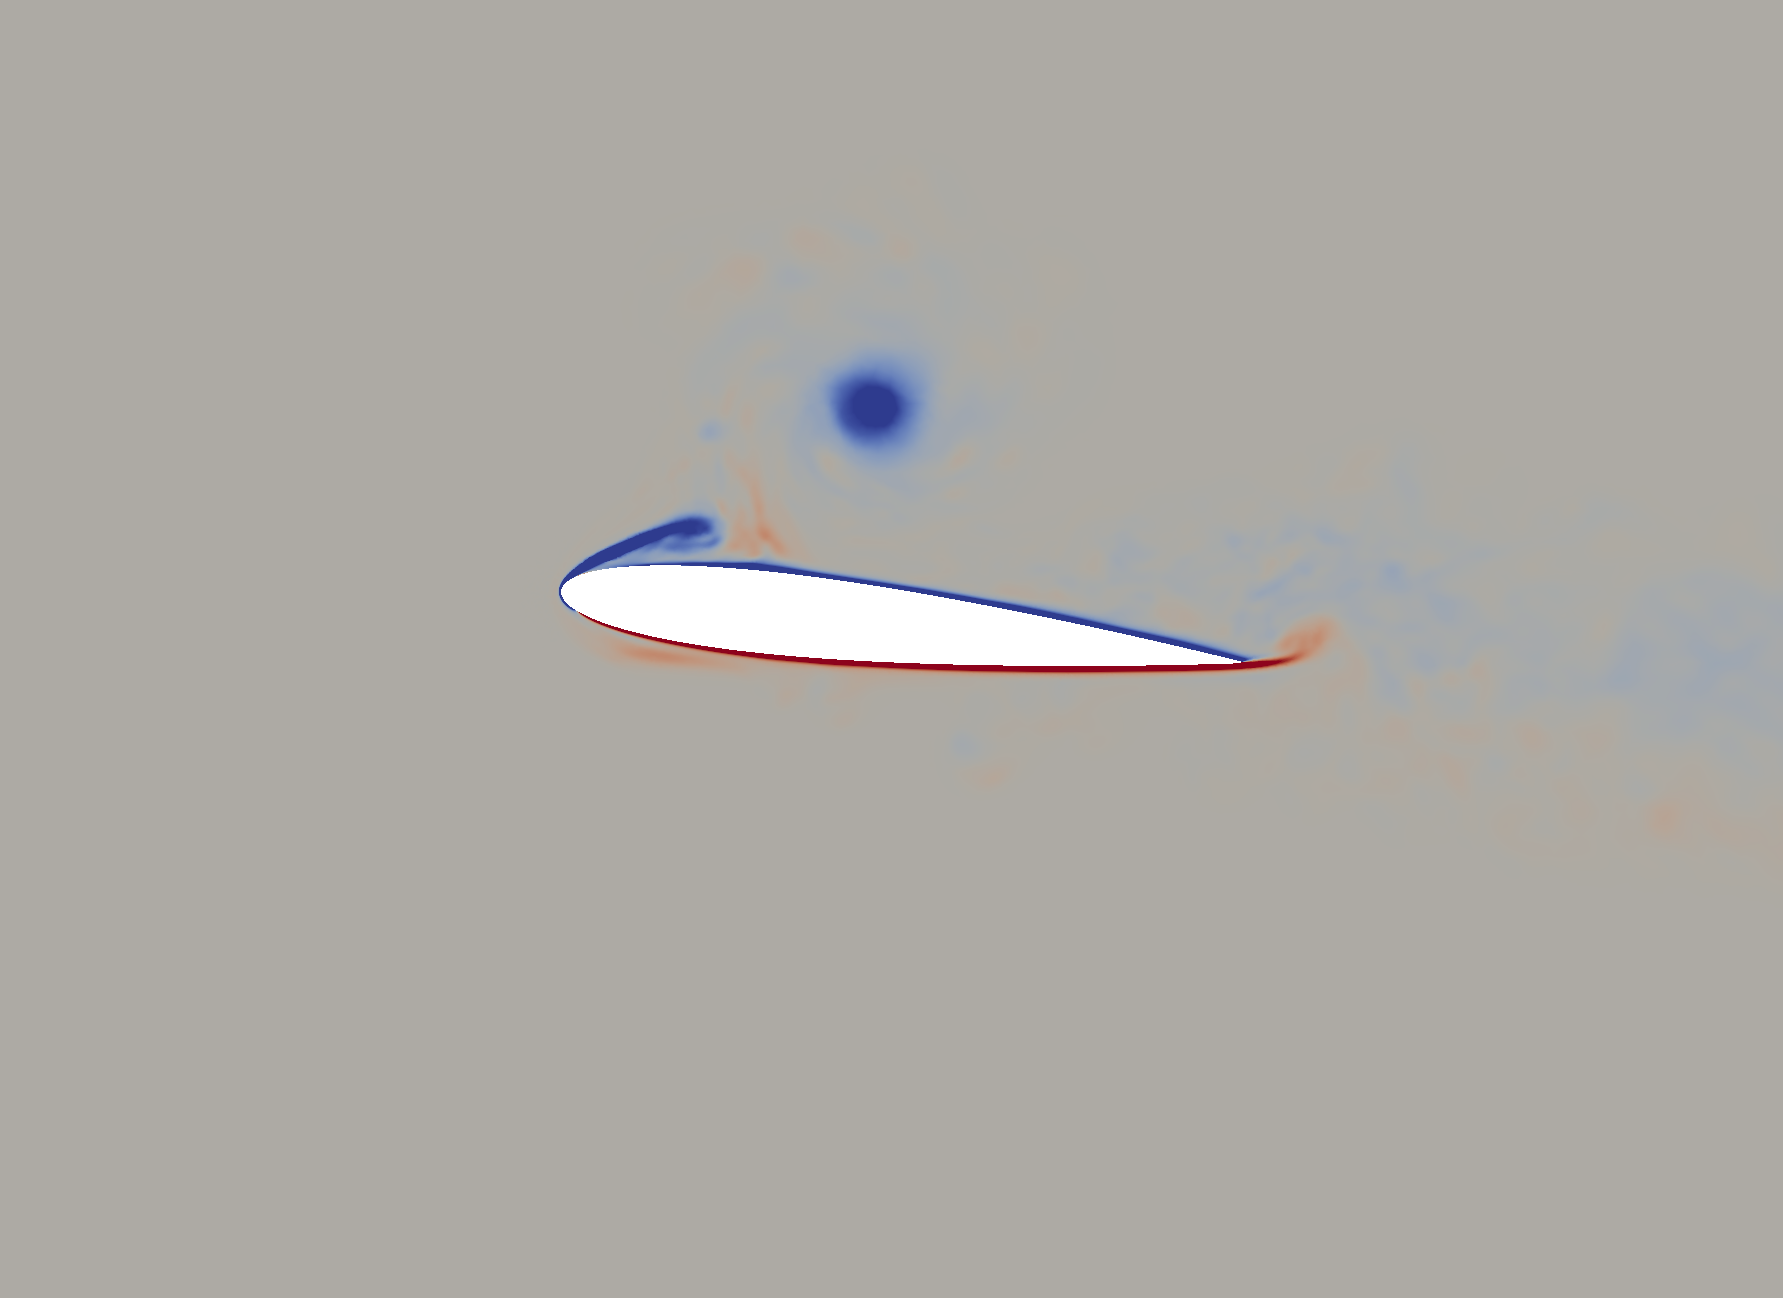
\includegraphics[width=1\textwidth]{figures/Vorticity_plots/Re_40k_1pt0/phase_315.png}
		\caption{$Re=4e4$, $\psi$ = $315^\circ$, $\tilde{t}=0.875$}
		\label{fig:Re_40k_1pt0_phi315}
	\end{subfigure}
	\begin{subfigure}[b]{0.32\textwidth}
		\centering
		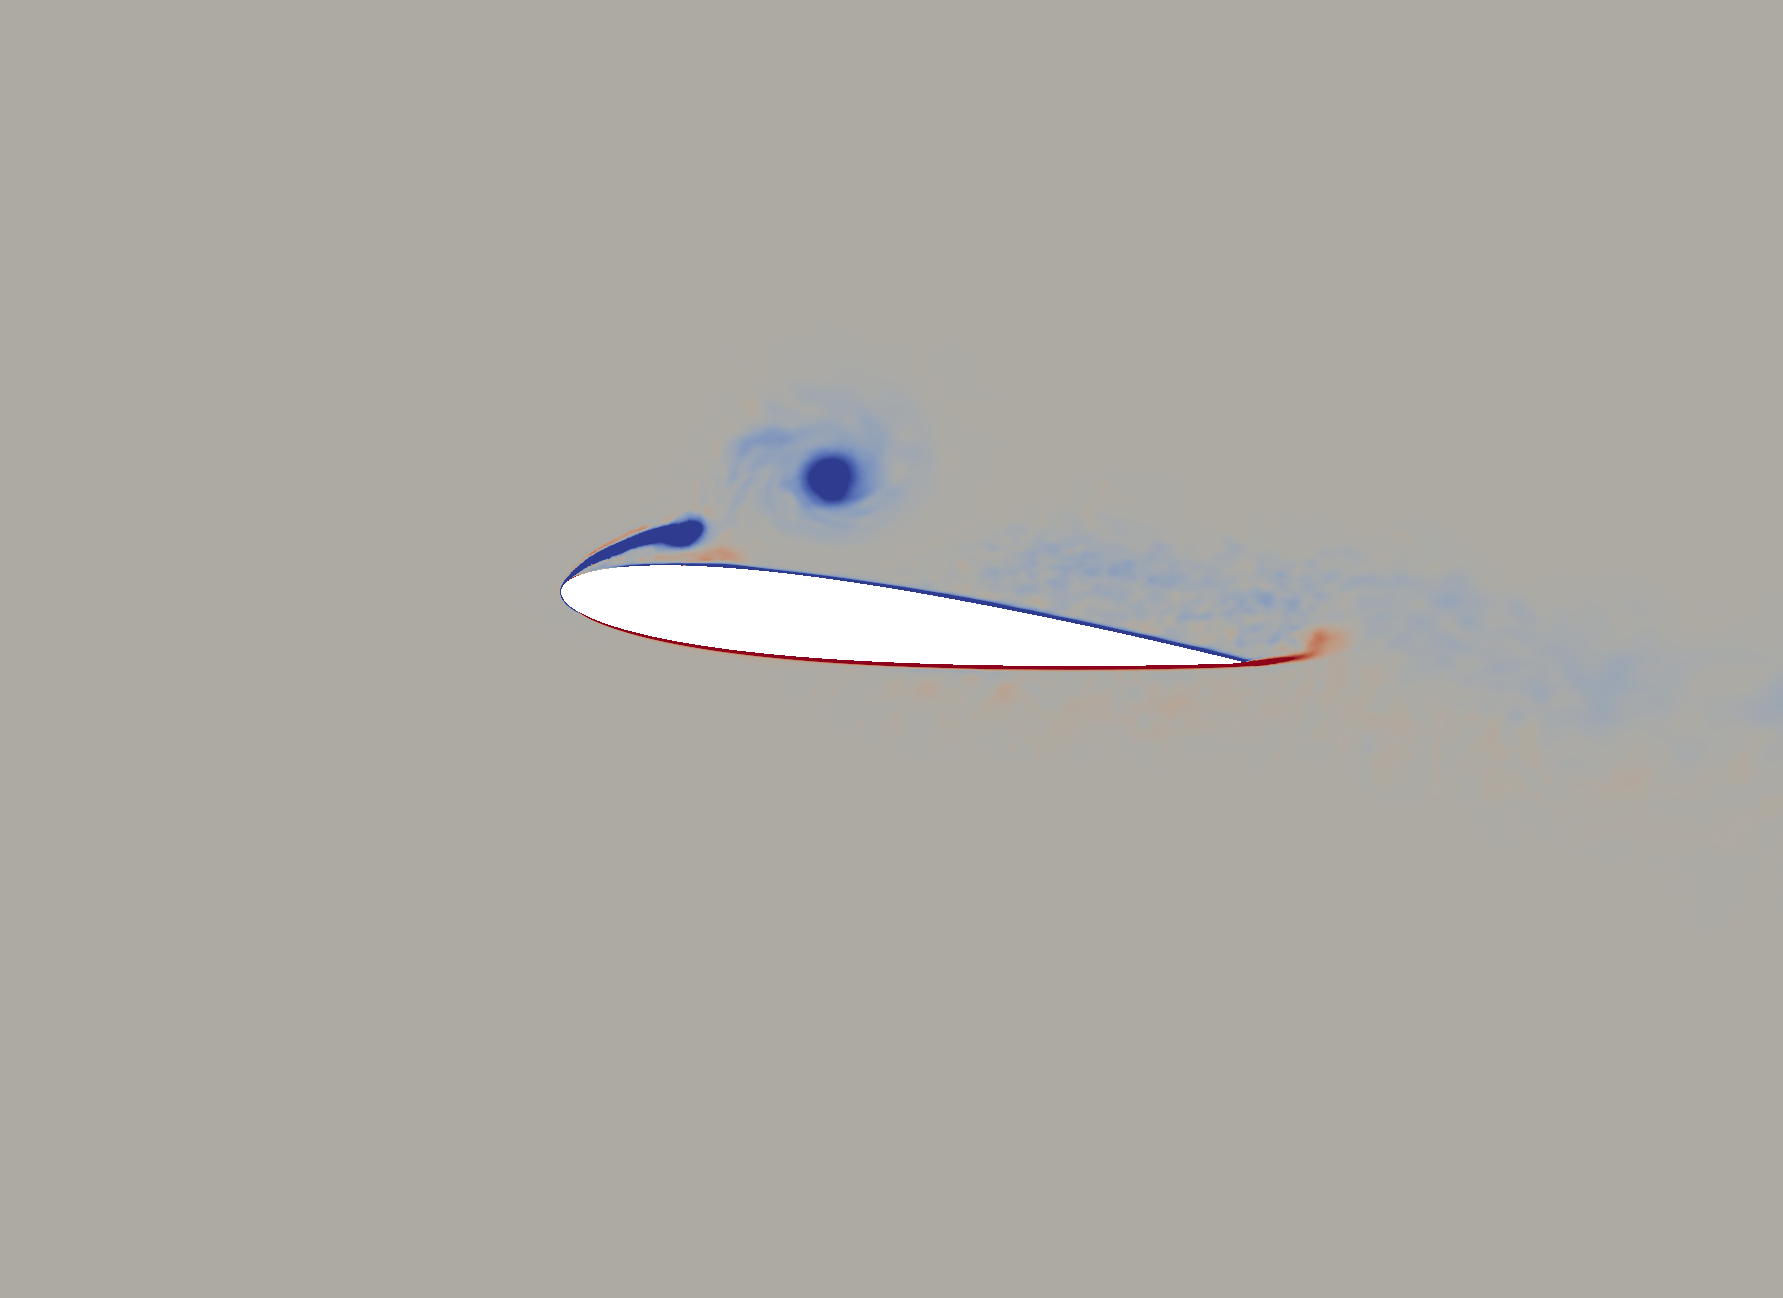
\includegraphics[width=1\textwidth]{figures/Vorticity_plots/Re_200k_1pt0/phase_315.png}
		\caption{$Re=2e5$, $\psi$ = $315^\circ$, $\tilde{t}=0.875$}
		\label{fig:Re_200k_1pt0_phi315}
	\end{subfigure}
	\begin{subfigure}[b]{0.32\textwidth}
		\centering
		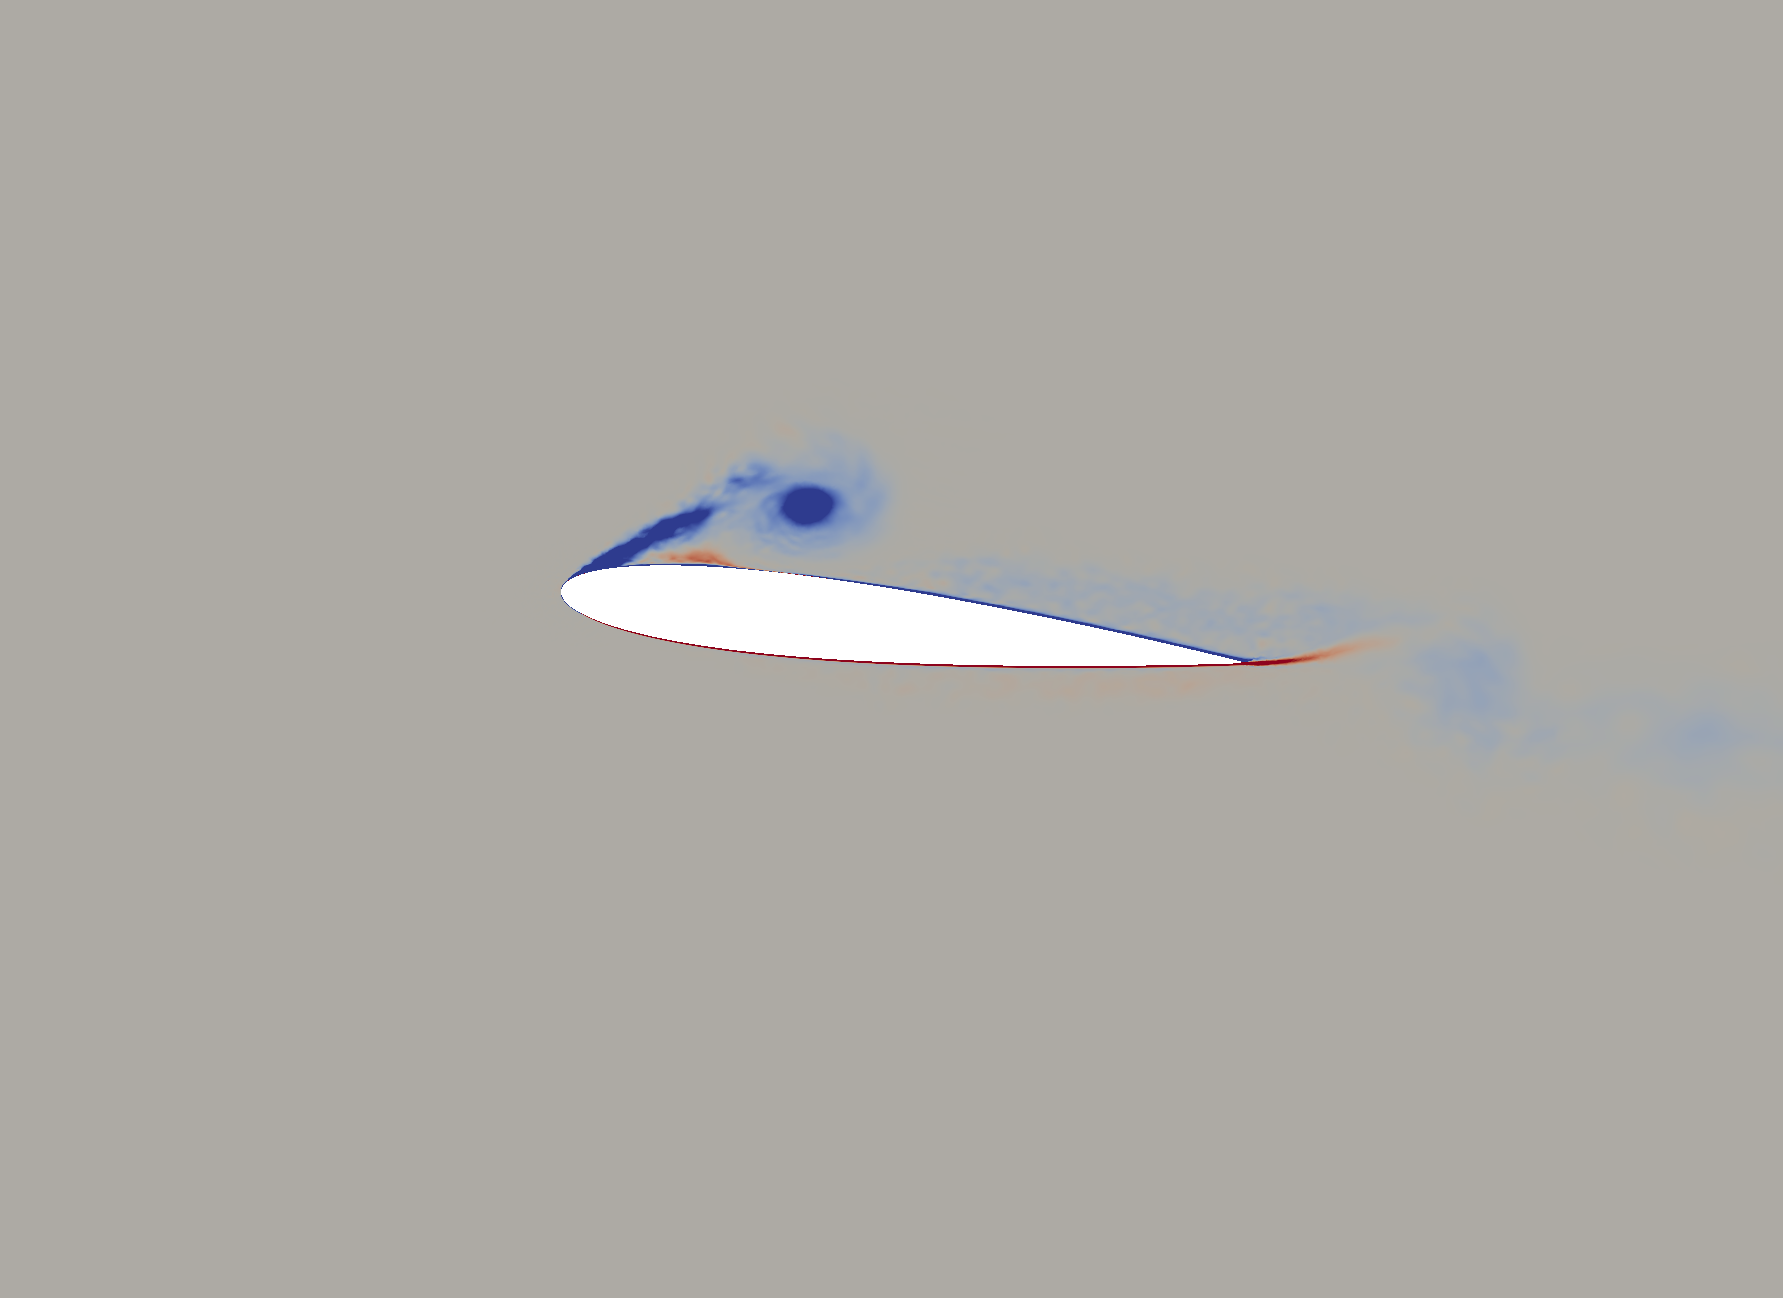
\includegraphics[width=1\textwidth]{figures/Vorticity_plots/Re_1m_1pt0/phase_315.png}
		\caption{$Re=1e6$, $\psi$ = $315^\circ$, $\tilde{t}=0.875$}
		\label{fig:Re_1m_1pt0_phi315}
	\end{subfigure}
	
	\begin{subfigure}[b]{0.32\textwidth}
		\centering
		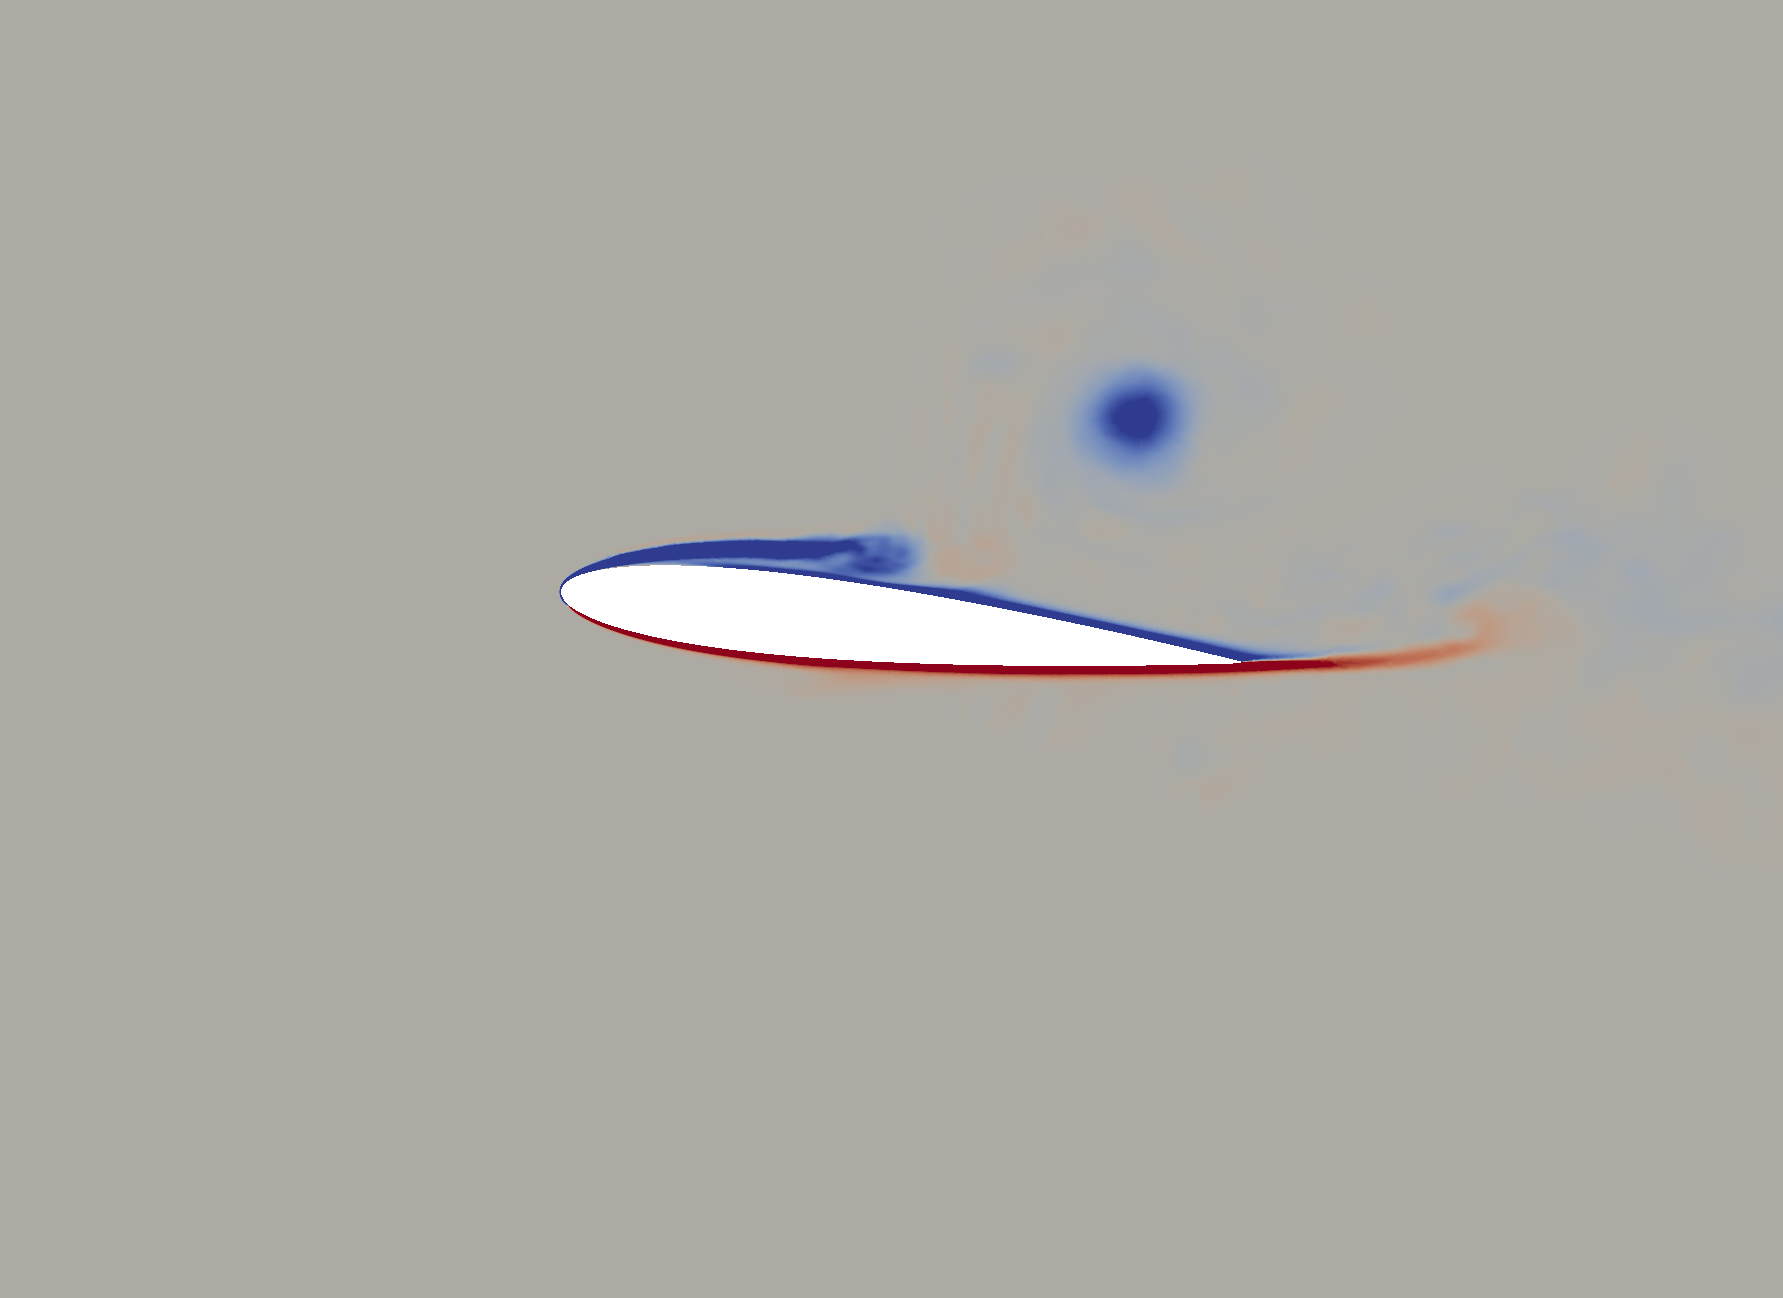
\includegraphics[width=1\textwidth]{figures/Vorticity_plots/Re_40k_1pt0/phase_330.png}
		\caption{$Re=4e4$, $\psi$ = $330^\circ$, $\tilde{t}=0.917$}
		\label{fig:Re_40k_1pt0_phi330}
	\end{subfigure}
	\begin{subfigure}[b]{0.32\textwidth}
		\centering
		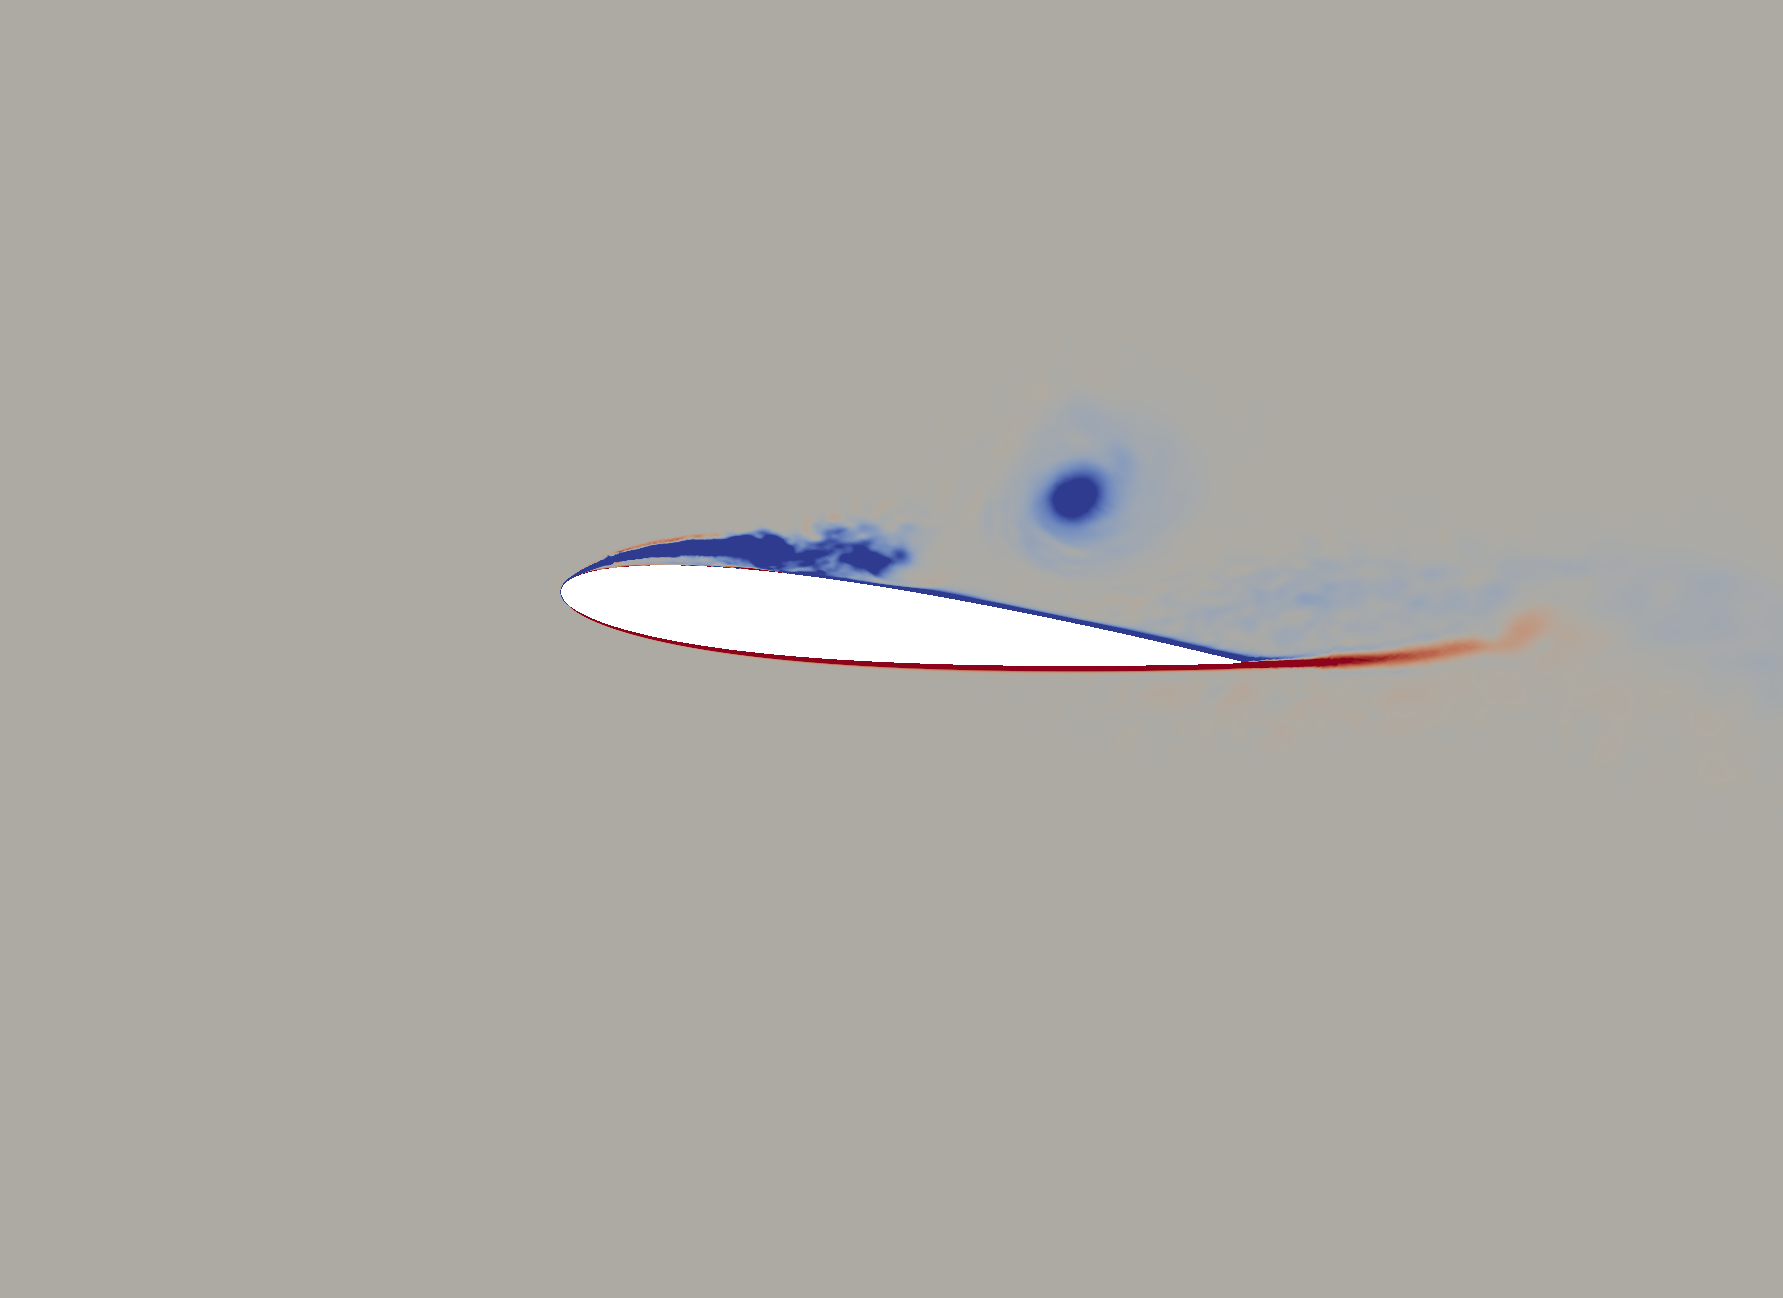
\includegraphics[width=1\textwidth]{figures/Vorticity_plots/Re_200k_1pt0/phase_330.png}
		\caption{$Re=2e5$, $\psi$ = $330^\circ$, $\tilde{t}=0.917$}
		\label{fig:Re_200k_1pt0_phi330}
	\end{subfigure}
	\begin{subfigure}[b]{0.32\textwidth}
		\centering
		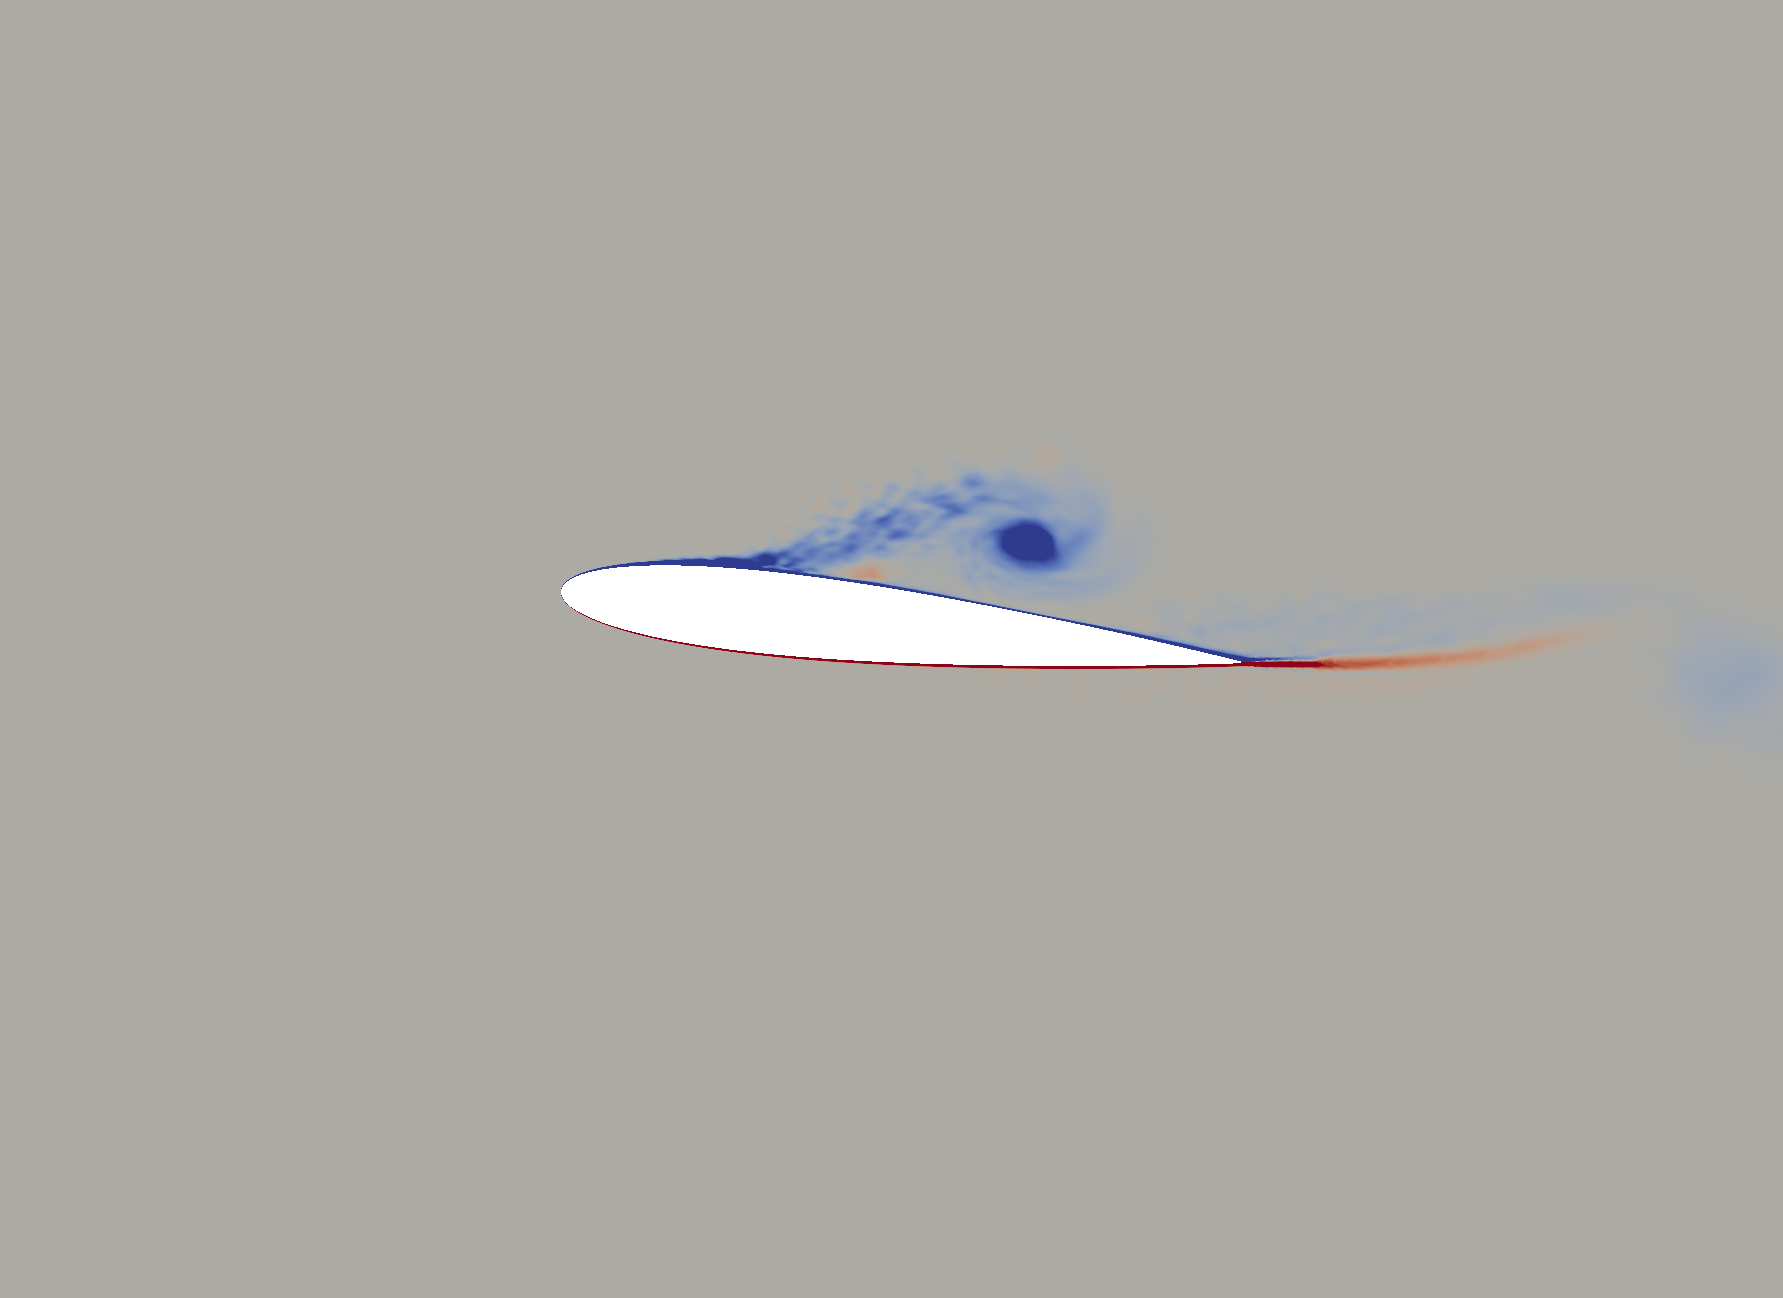
\includegraphics[width=1\textwidth]{figures/Vorticity_plots/Re_1m_1pt0/phase_330.png}
		\caption{$Re=1e6$,$\psi$ = $330^\circ$, $\tilde{t}=0.917$}
		\label{fig:Re_1m_1pt0_phi330}
	\end{subfigure}
	
	\begin{subfigure}[b]{0.32\textwidth}
		\centering
		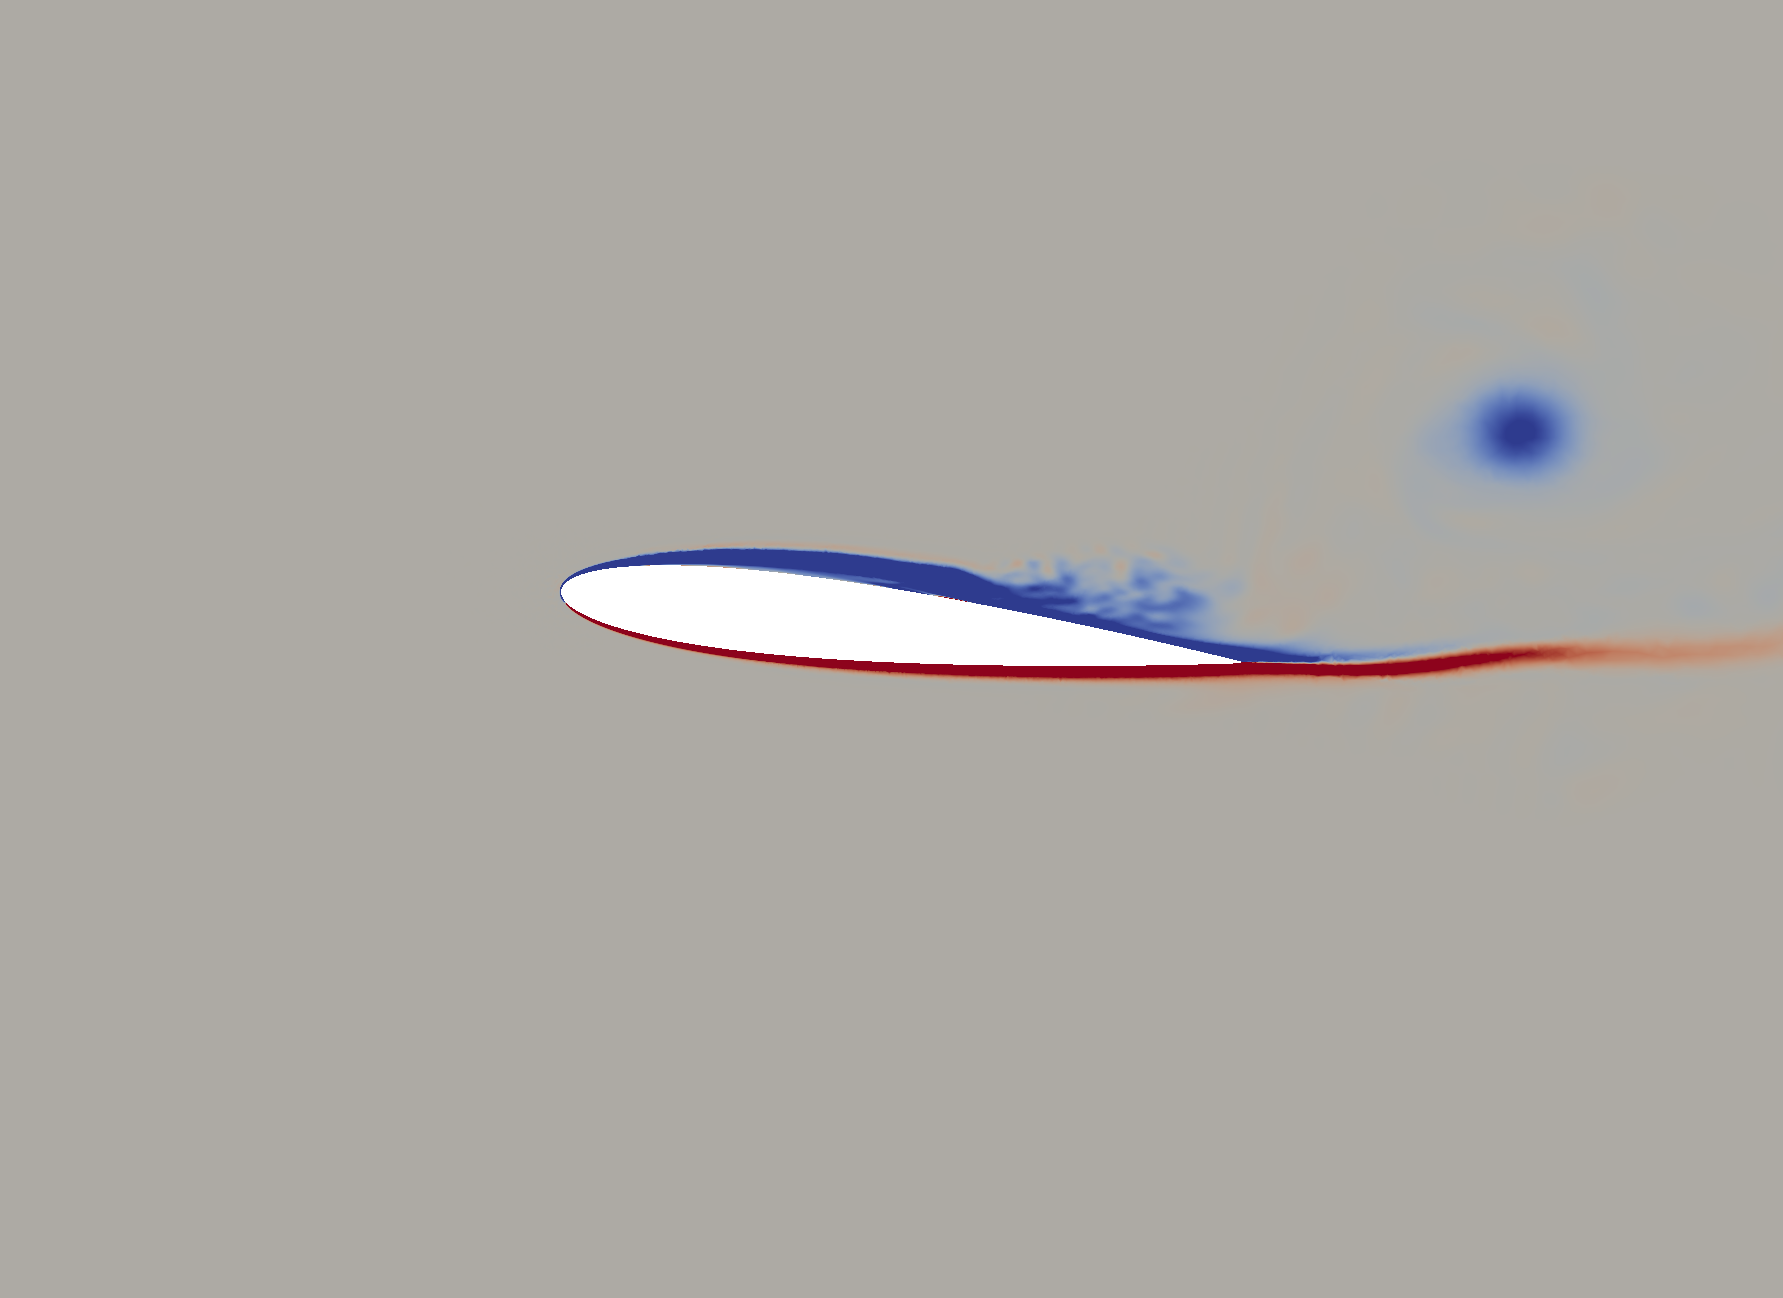
\includegraphics[width=1\textwidth]{figures/Vorticity_plots/Re_40k_1pt0/phase_345.png}
		\caption{$Re=4e4$, $\psi$ = $345^\circ$, $\tilde{t}=0.958$}
		\label{fig:Re_40k_1pt0_phi345}
	\end{subfigure}
	\begin{subfigure}[b]{0.32\textwidth}
		\centering
		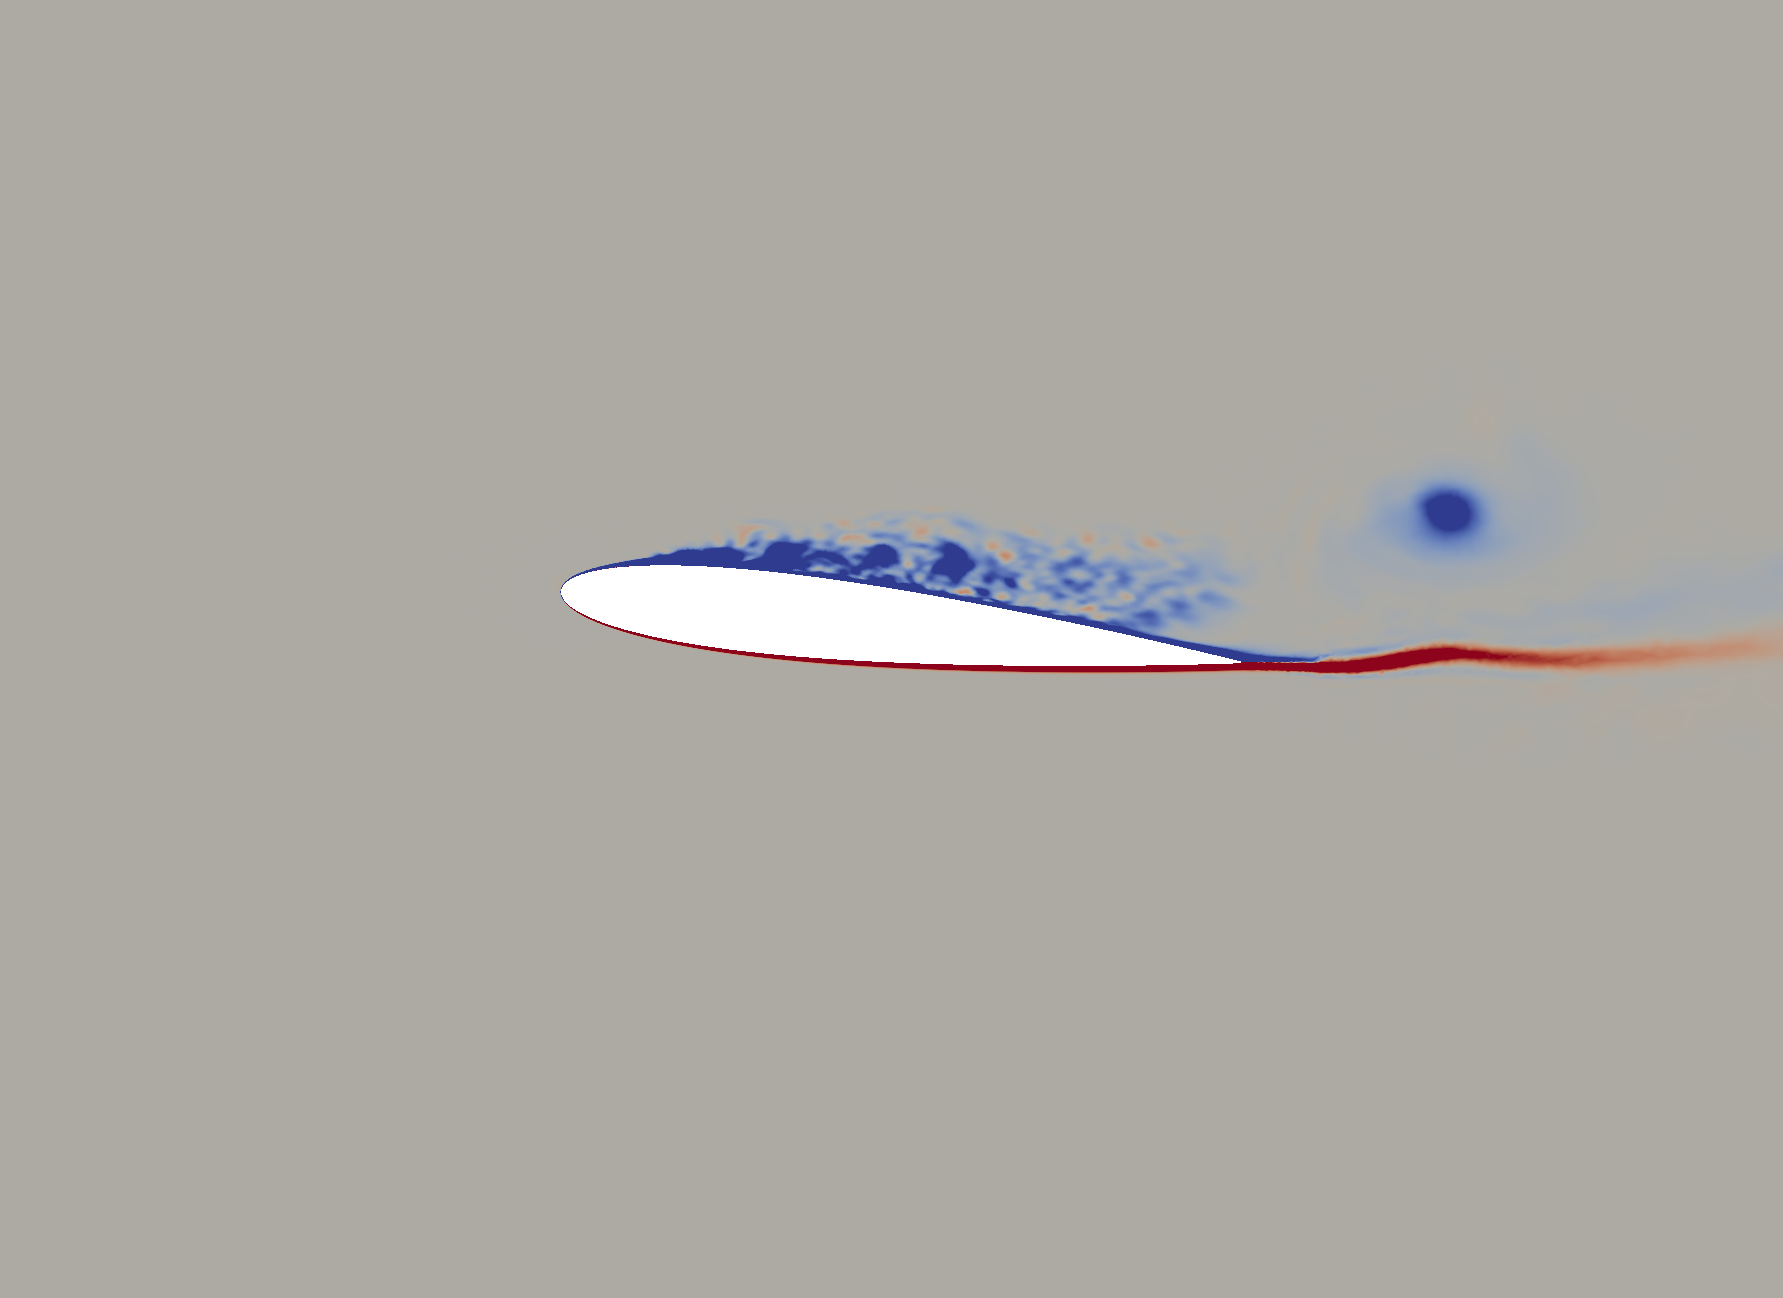
\includegraphics[width=1\textwidth]{figures/Vorticity_plots/Re_200k_1pt0/phase_345.png}
		\caption{$Re=2e5$, $\psi$ = $345^\circ$, $\tilde{t}=0.958$}
		\label{fig:Re_200k_1pt0_phi345}
	\end{subfigure}
	\begin{subfigure}[b]{0.32\textwidth}
		\centering
		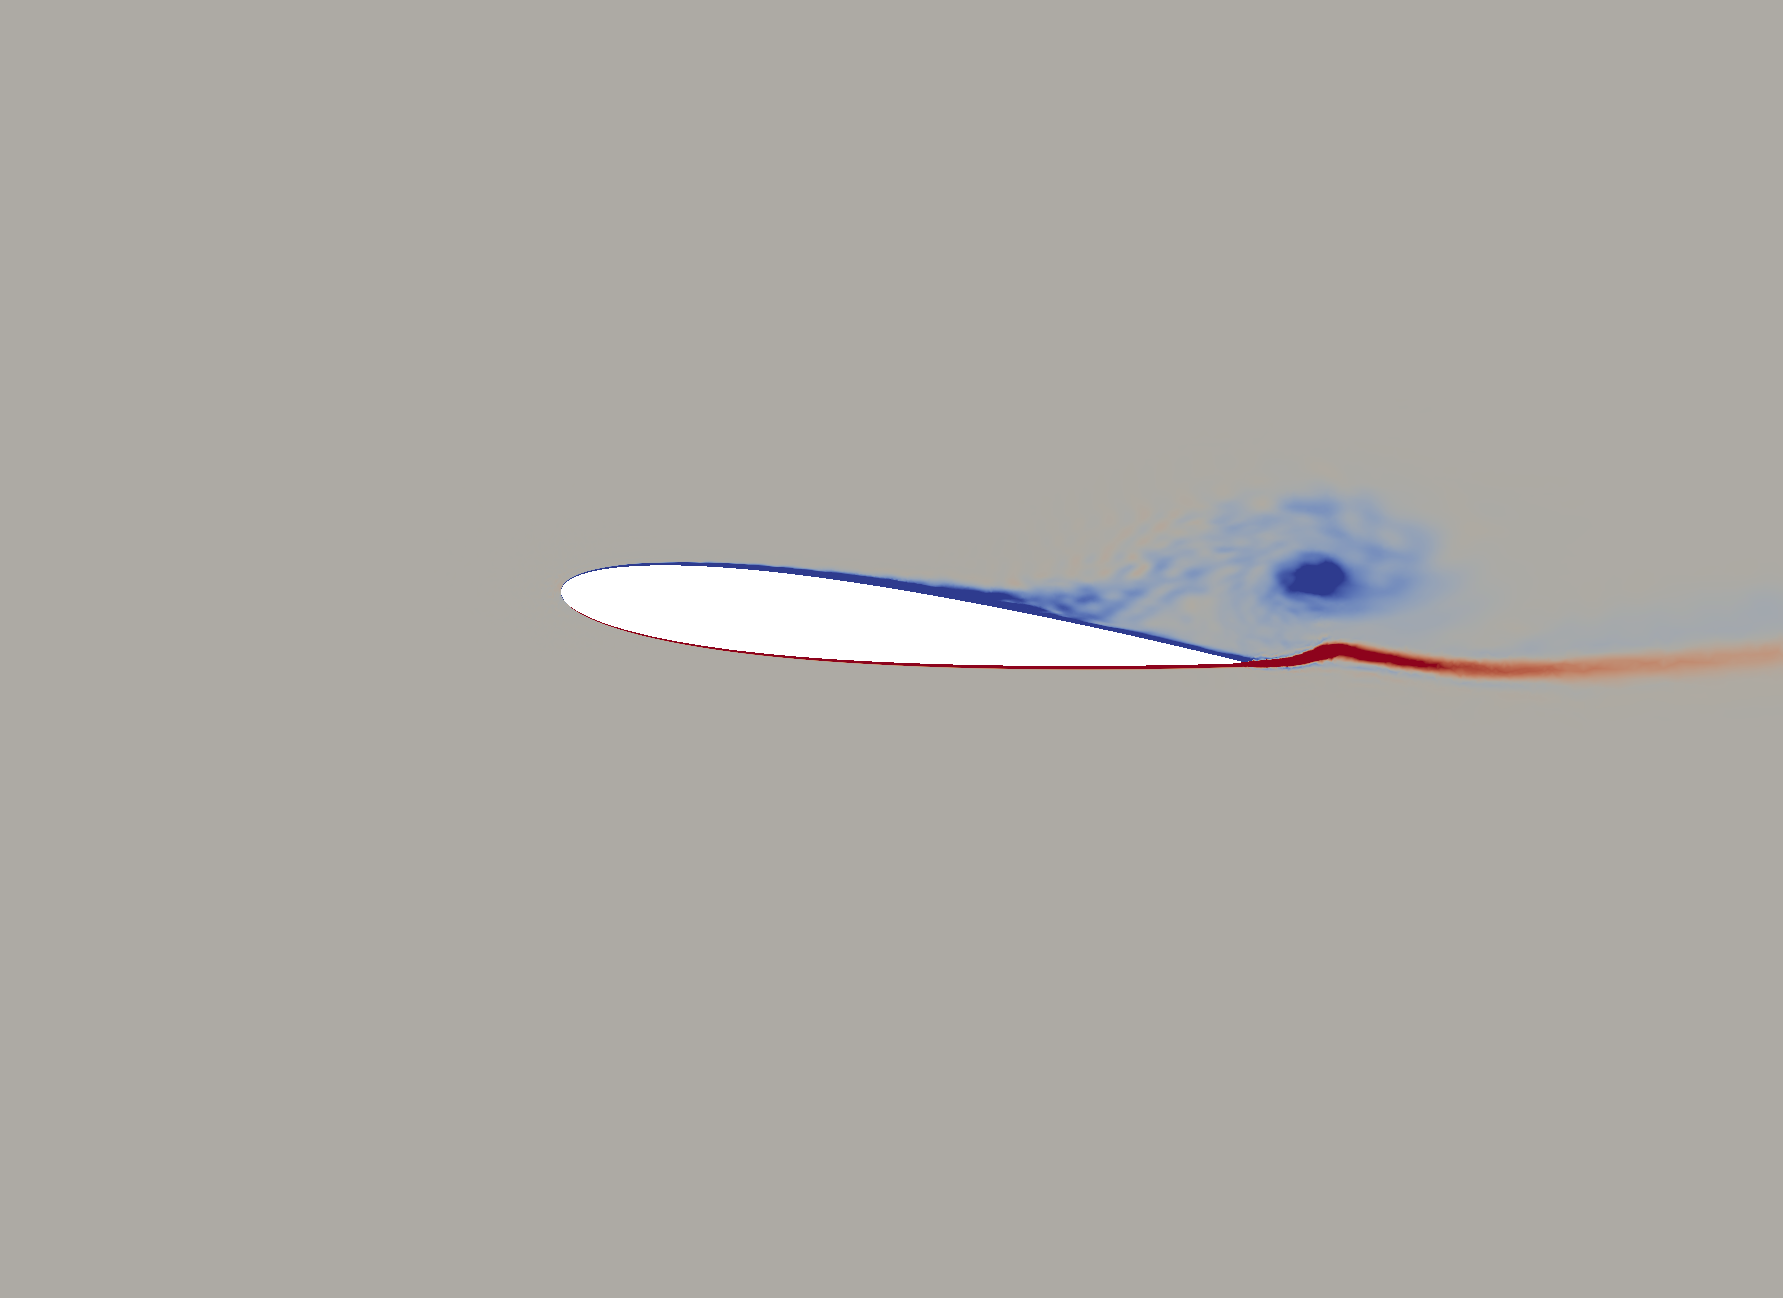
\includegraphics[width=1\textwidth]{figures/Vorticity_plots/Re_1m_1pt0/phase_345.png}
		\caption{$Re=1e6$, $\psi$ = $345^\circ$, $\tilde{t}=0.958$}
		\label{fig:Re_1m_1pt0_phi345}
	\end{subfigure}	
\caption{Spanwise vorticity at 8 different phases for $Re$=40,000 (left column), 200,000 (middle column) and 1,000,000 (right column) at $\mu_{sect}$ = 1.0}
\label{fig:vortScreen_1pt0}
\end{figure}


At $\psi$=$225^\circ$, the flow is separated near the leading edge for the lowest Reynolds number of $Re$=40,000 and the separated shear layer rolls up into an LEV, see Figure~\ref{fig:Re_200k_1pt0_phi225}.
For the other two higher Reynolds numbers, the flow remains attached.
Similarly, at $Re$=200,000 the separated shear layer rolls up into a smaller LEV at $\psi$=$240^\circ$, while for $Re$=1,000,000 this occurs at $\psi$=$270^\circ$ (see Figure \ref{fig:Re_1m_1pt0_phi270}).
As the Reynolds number increases the LEV is formed later in the cycle.
In summary, as the airfoil retreats vorticity accumulates around the airfoil and separated shear layer rolls up into a distinct vortex near the leading edge (i.e., an LEV) over the suction or upper side of the airfoil.

In subsequent phases, LEV is ejected into the outer flow and advects.
The flow on the suction or upper side reattaches as the leading edge vortex passes over the airfoil.
Flow also separates and reattaches on the pressure or lower side, e.g., see marginal flow separation at the trailing edge on the lower side in Fig \ref{fig:Re_40k_1pt0_phi225}.

It is important to note the differences in LEV evolution with different Reynolds number even though the overall trend of the LEV evolution is similar between different Reynolds number.
As already noted, the phase at which the LEV is formed changes with Reynolds number.
Further, the size and vertical position of the LEV also changes significantly with Reynolds number.
This aspect is discussed in Section \ref{sec:LEV}.

Figure \ref{fig:vortScreen_1pt2} shows the spanwise vorticity for the higher advance ratio of $\mu_{sect}$=1.2.
Again, 8 different phases over the retreating phase of the cycle are shown and the range is selected to be [-10,10]$\times U_\infty /C$.
As in the $\mu_{sect}=1.0$ case, at $\psi$=$195^\circ$ the flow over the airfoil is mostly attached in the $\mu_{sect}=1.2$ case.
As before, the boundary layer is much thicker for the lowest Reynolds number of $Re$=40,000 as compared to the other two higher Reynolds numbers.

At $\psi$=$225^\circ$, the flow is fully separated for the lowest Reynolds number of $Re$=40,000 and the separated shear layer is rolled up into an LEV, see Figure~\ref{fig:Re_40k_1pt2_phi225}.
Similarly, at $Re$=200,000 a smaller LEV is seen at $\psi$=$225^\circ$ (see Figure \ref{fig:Re_200k_1pt2_phi225}), while for $Re$=1,000,000, LEV is observed at $\psi$=$240^\circ$.
As before, as the Reynolds number increases the LEV is formed later in the cycle.
On the other hand, as the advance ratio increases it is formed earlier in the cycle (for a given Reynolds number).
For example, for $Re$=1,000,000, the LEV is formed at an earlier phase for $\mu_{sect}=1.2$ as compared to $\mu_{sect}=1.0$.
Again, as the airfoil retreats vorticity accumulates and shear layer rolls up into a distinct LEV over the suction or upper side of the airfoil.

In subsequent phases, LEV is ejected into the outer flow and advects while the flow reattaches.
However, at the higher advance ratio of $\mu_{sect}$=1.2 the LEV initially moves to the left past the (geometric) leading edge of the airfoil.
This is because at $\mu_{sect}$=1.2, the relative flow velocity becomes negative and a reversed flow condition is reached.
Again, it is important to note the differences in LEV evolution with different Reynolds number for the advance ratio of $\mu_{sect}=1.2$.
As already noted, the size, position and phase of formation of LEV changes significantly with Reynolds number.
This aspect is discussed further in Section \ref{sec:LEV}.

\begin{figure}[H]
	\centering
	
	\begin{subfigure}[b]{0.32\textwidth}
		\centering
		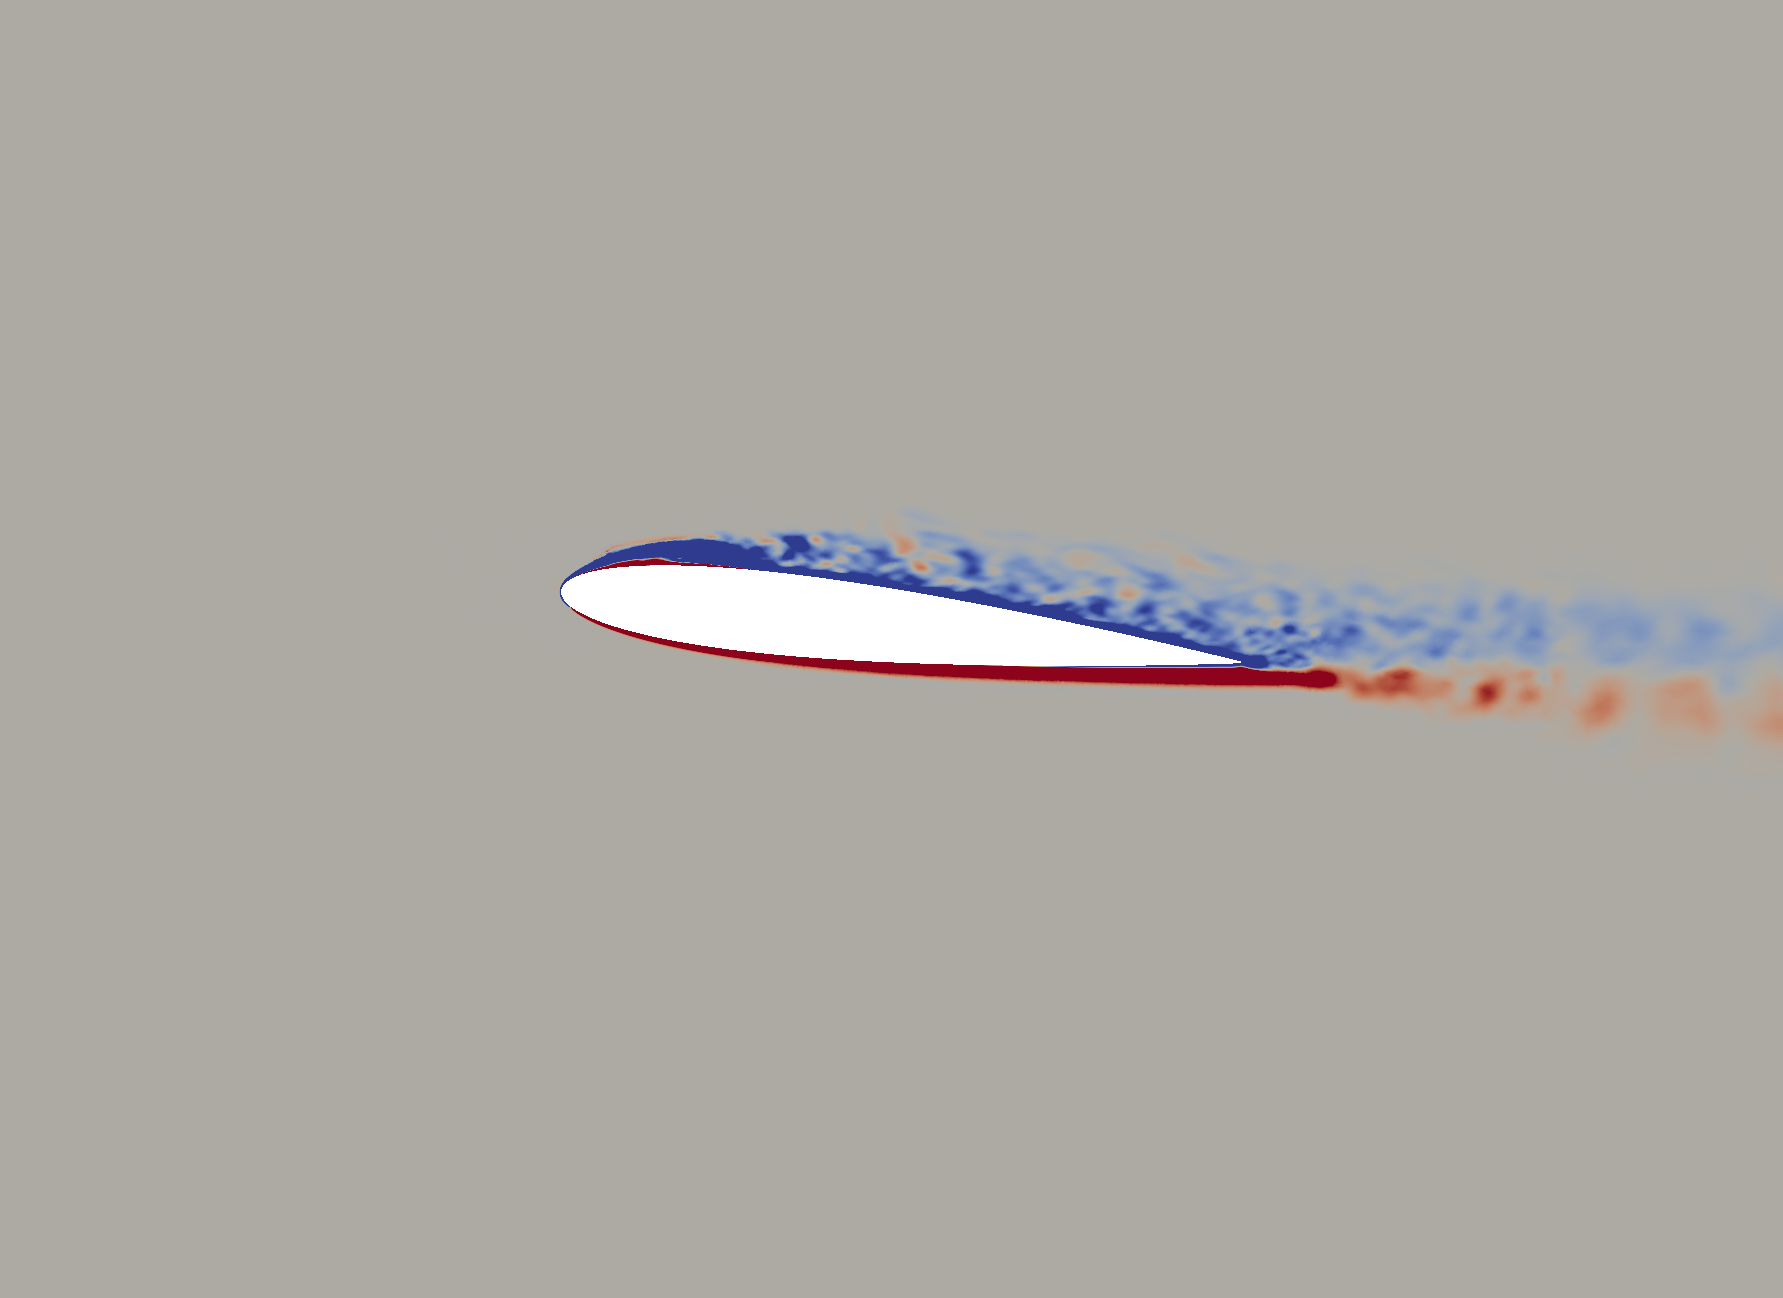
\includegraphics[width=1\textwidth]{figures/Vorticity_plots/Re_40k_1pt2/phase_195.png}
		\caption{$Re= 4e4$, $\psi$ = $195^\circ$, $\tilde{t}=0.542$}
		\label{fig:Re_40k_1pt2_phi195}
	\end{subfigure}
	\begin{subfigure}[b]{0.32\textwidth}
		\centering
		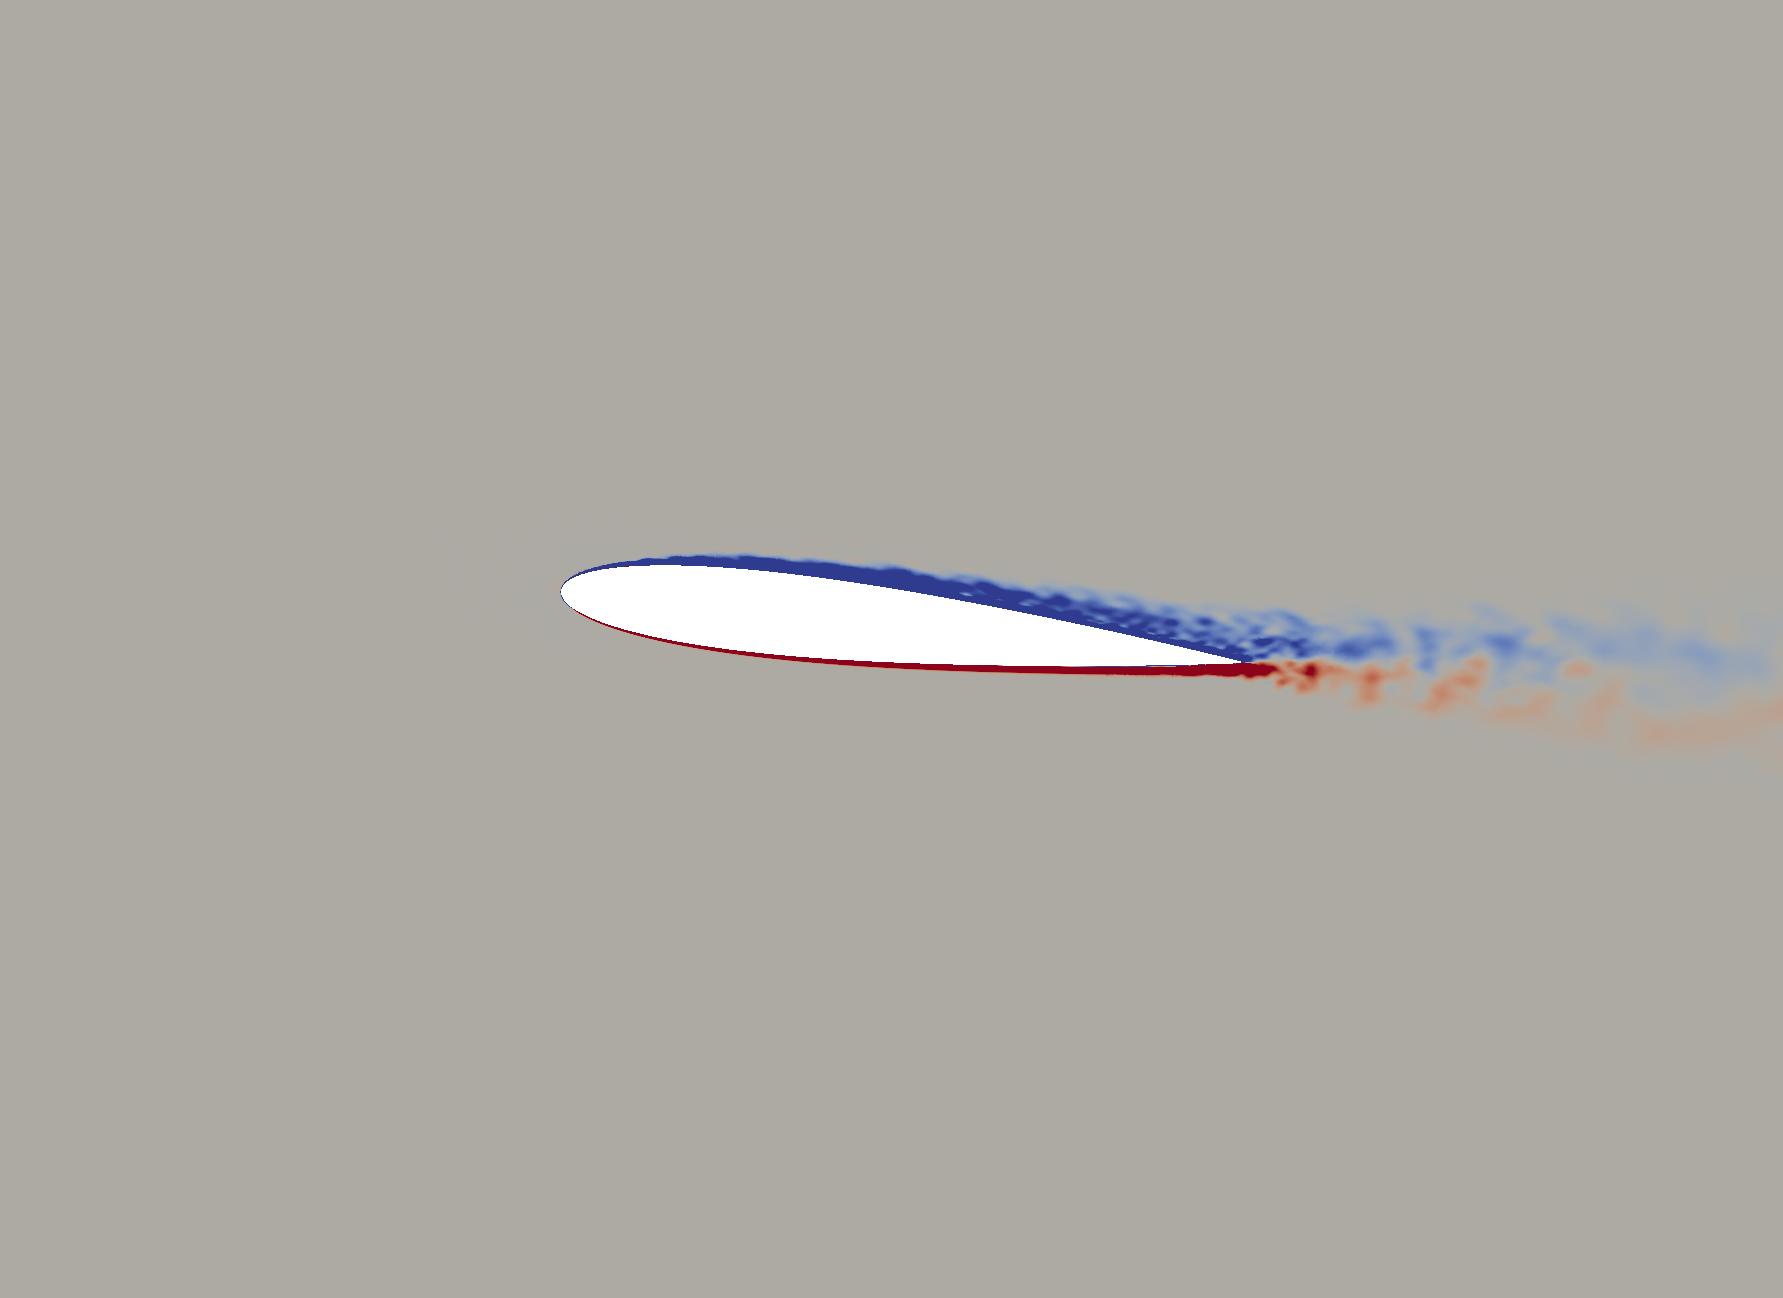
\includegraphics[width=1\textwidth]{figures/Vorticity_plots/Re_200k_1pt2/phase_195.png}
		\caption{$Re=2e5$, $\psi$ = $195^\circ$, $\tilde{t}=0.542$}
		\label{fig:Re_200k_1pt2_phi195}
	\end{subfigure}
	\begin{subfigure}[b]{0.32\textwidth}
		\centering
		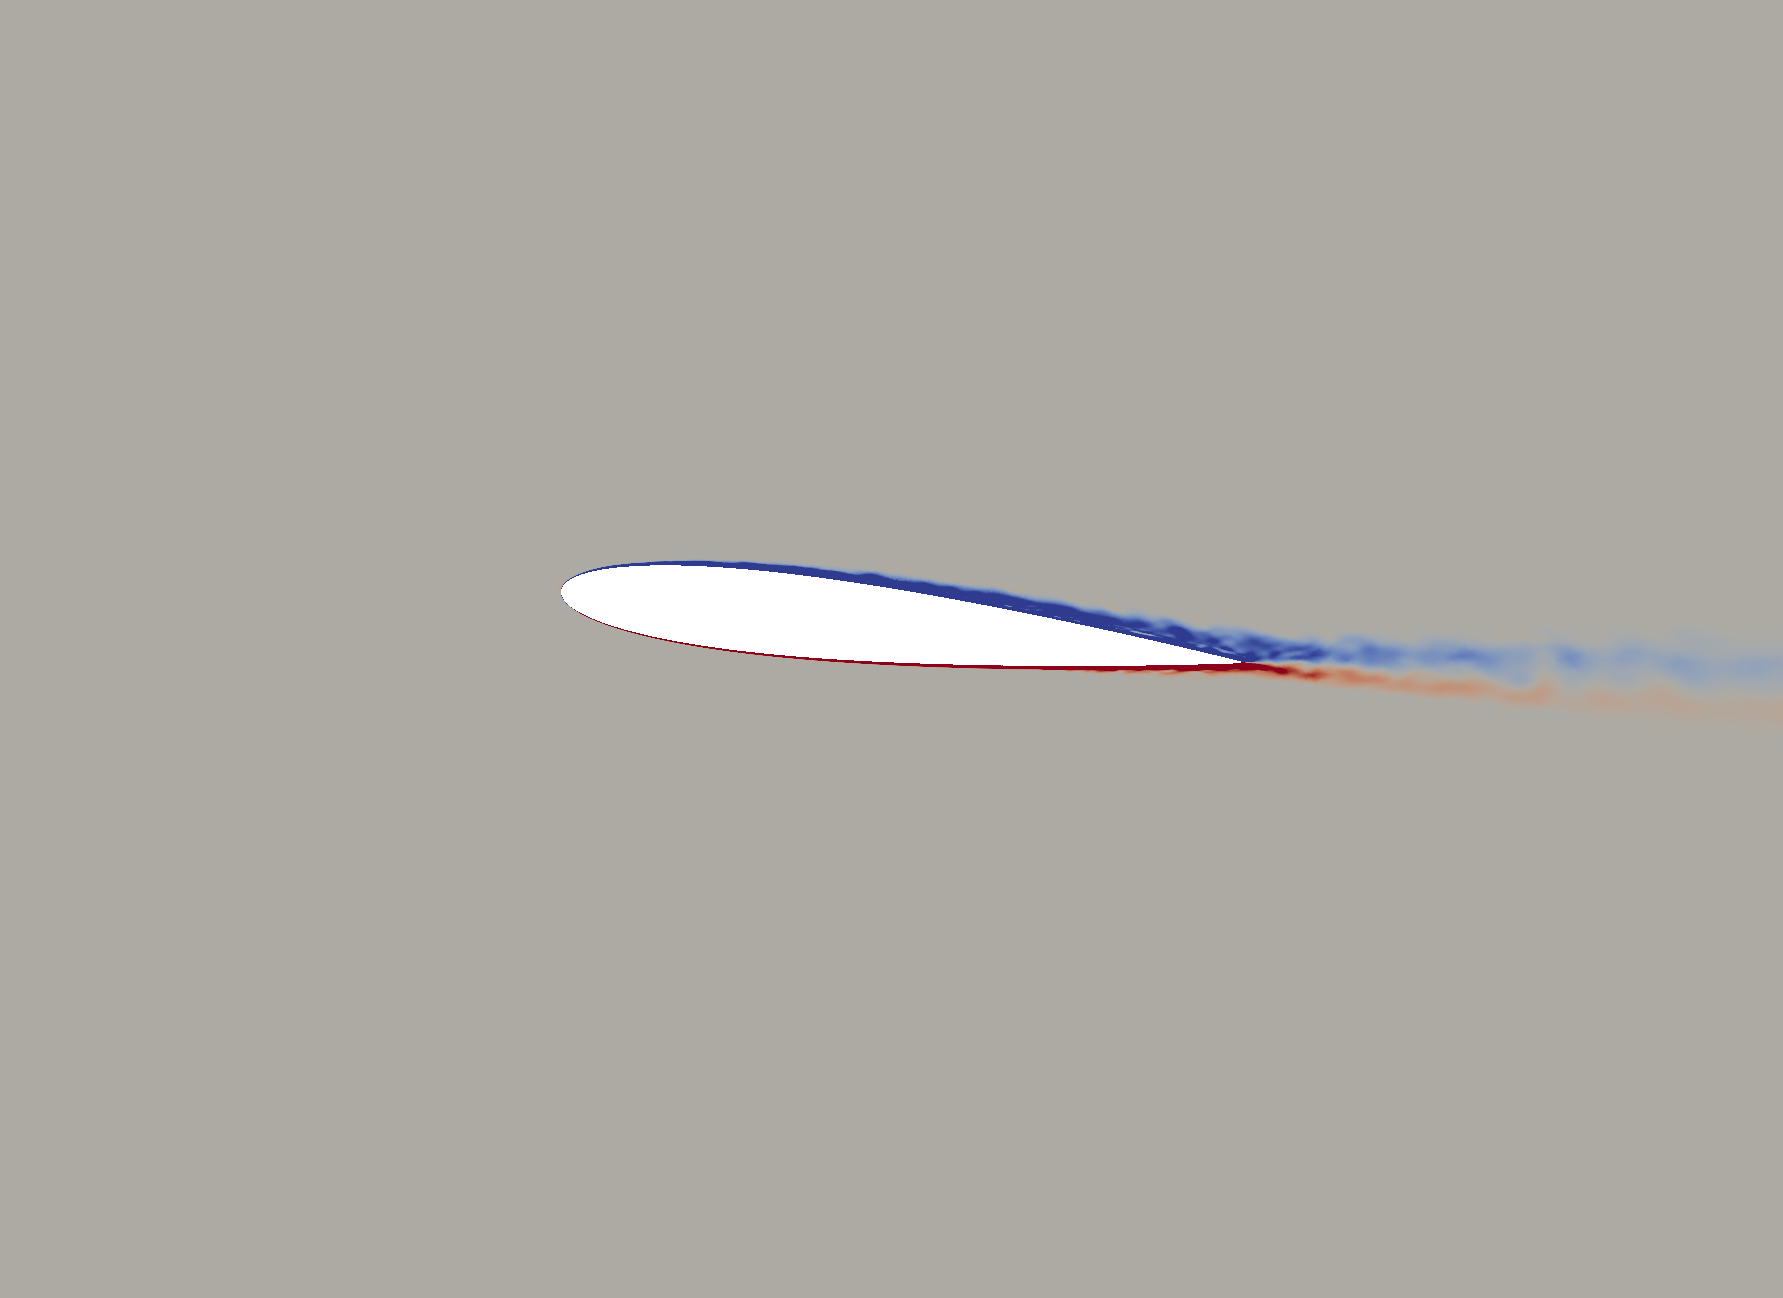
\includegraphics[width=1\textwidth]{figures/Vorticity_plots/Re_1m_1pt2/phase_195.png}
		\caption{$Re= 1e6$, $\psi$ = $195^\circ$, $\tilde{t}=0.542$}
		\label{fig:Re_1m_1pt2_phi195}
	\end{subfigure}
	
	\begin{subfigure}[b]{0.32\textwidth}
		\centering
		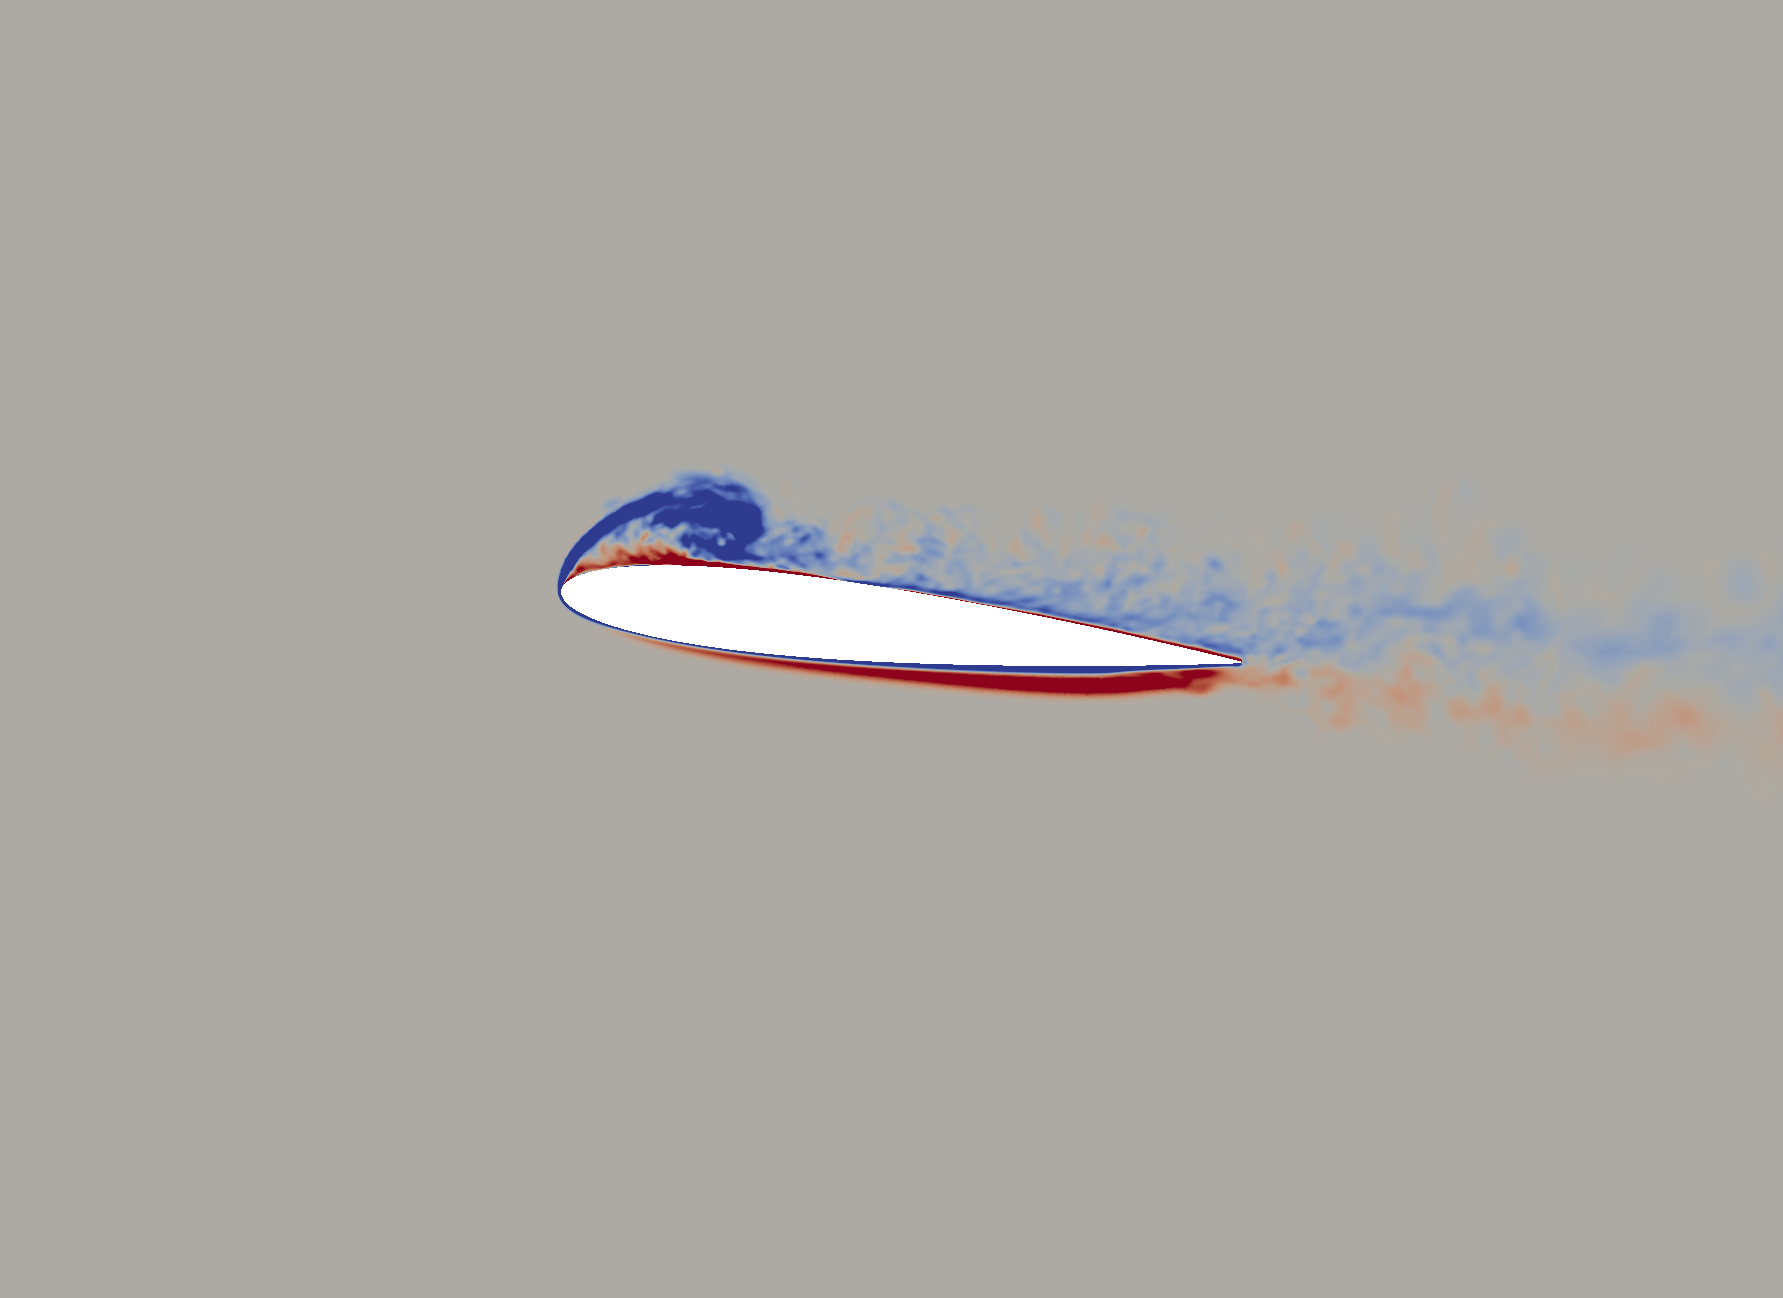
\includegraphics[width=1\textwidth]{figures/Vorticity_plots/Re_40k_1pt2/phase_225.png}
		\caption{$Re=4e4$, $\psi$ = $225^\circ$, $\tilde{t}=0.625$}
		\label{fig:Re_40k_1pt2_phi225}
	\end{subfigure}
	\begin{subfigure}[b]{0.32\textwidth}
		\centering
		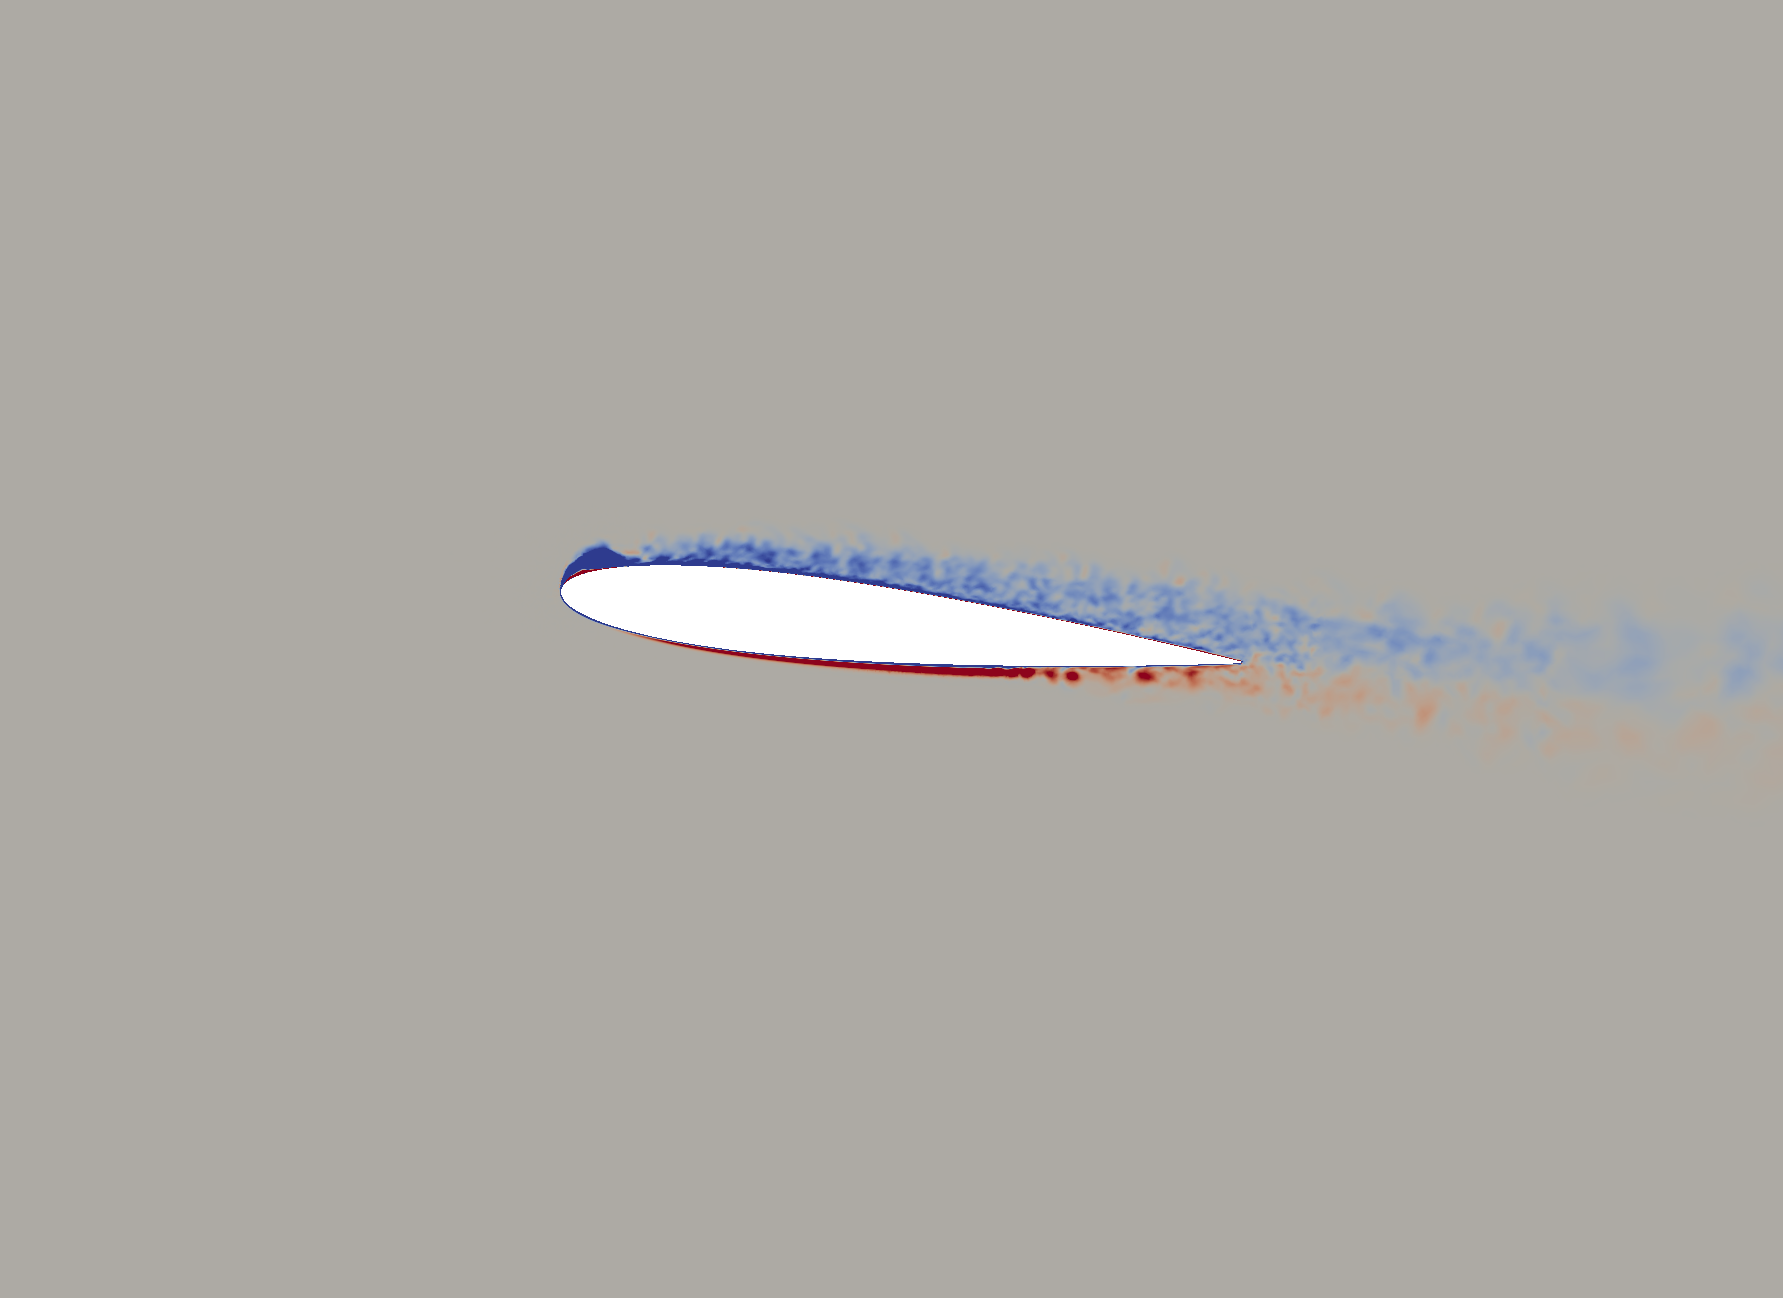
\includegraphics[width=1\textwidth]{figures/Vorticity_plots/Re_200k_1pt2/phase_225.png}
		\caption{$Re=2e5$, $\psi$ = $225^\circ$, $\tilde{t}=0.625$}
		\label{fig:Re_200k_1pt2_phi225}
	\end{subfigure}
	\begin{subfigure}[b]{0.32\textwidth}
		\centering
		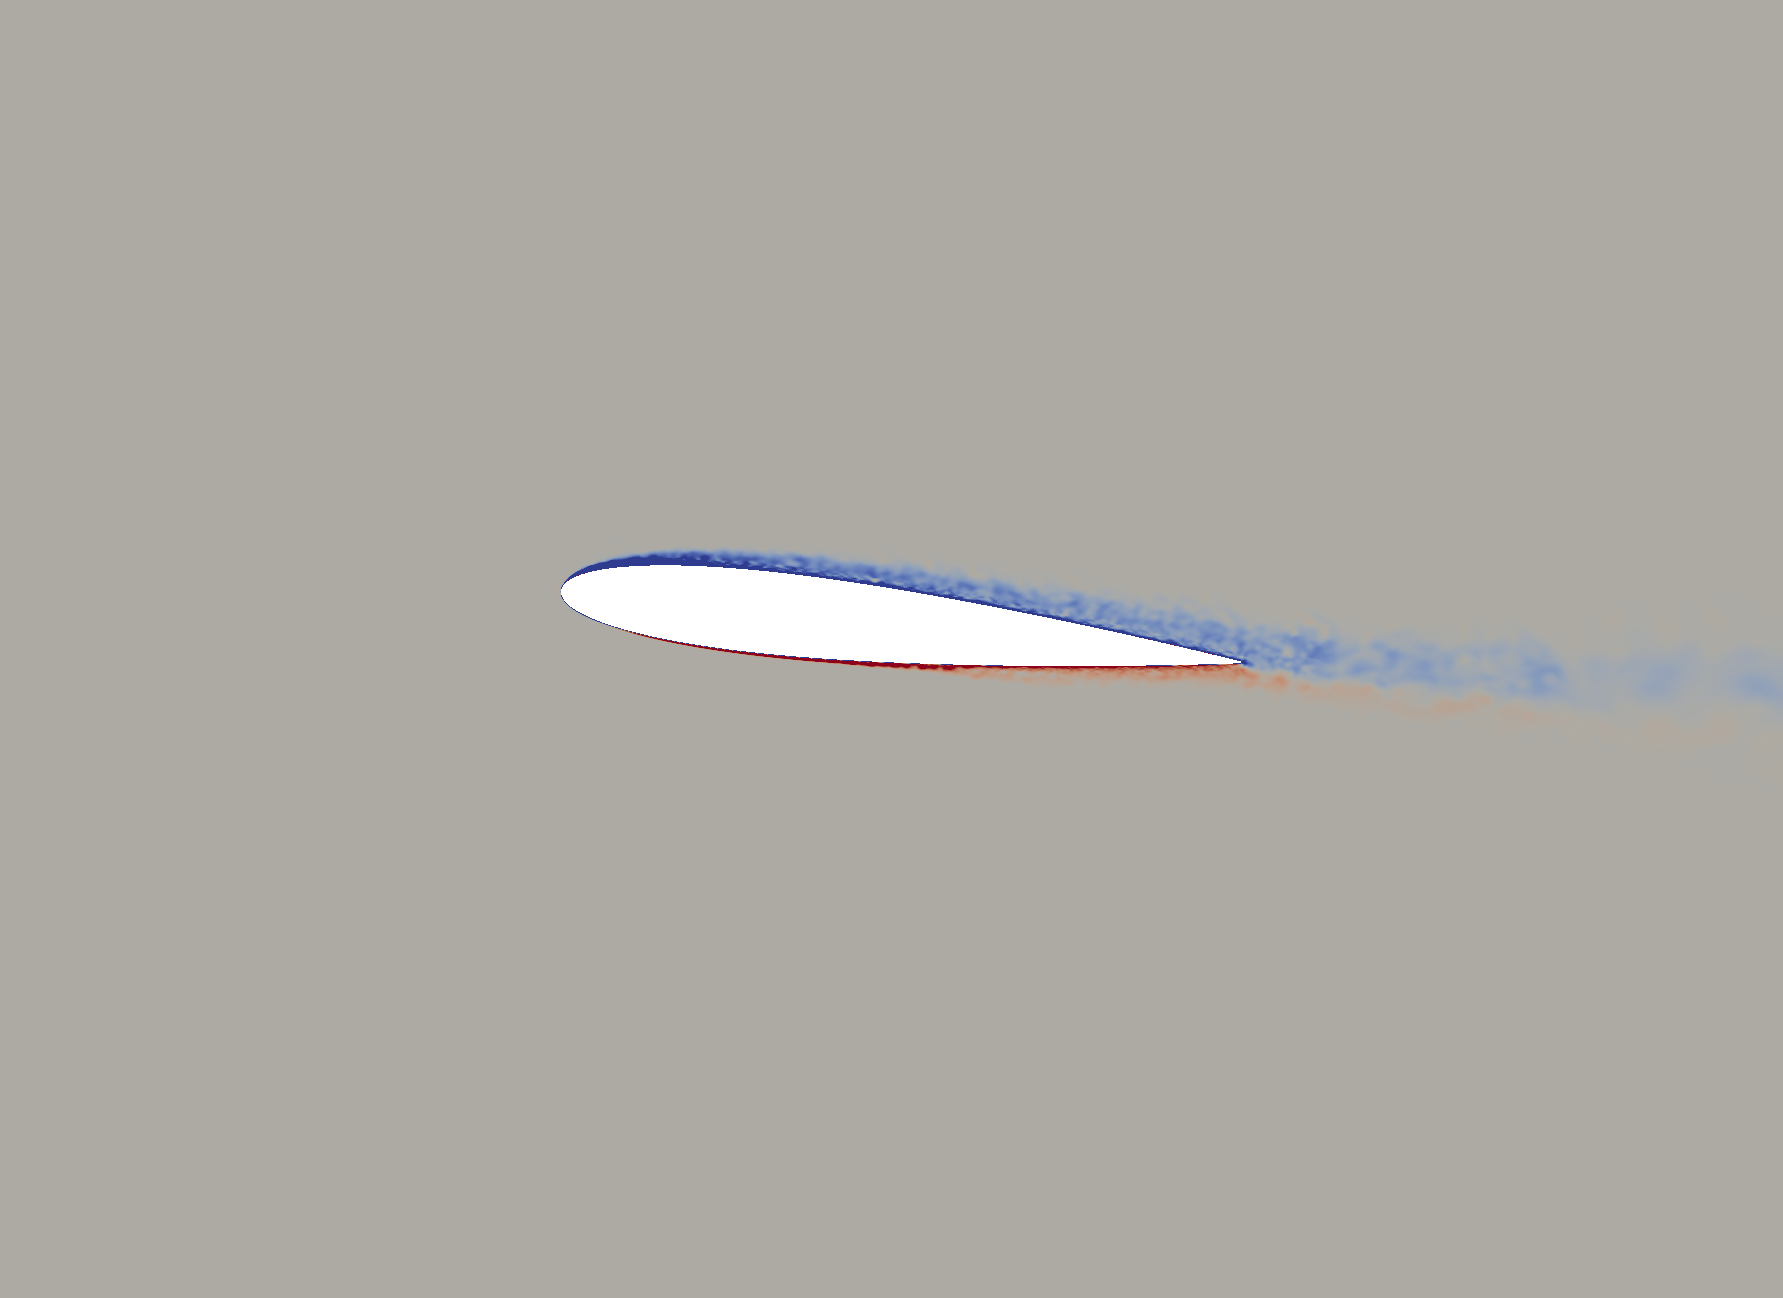
\includegraphics[width=1\textwidth]{figures/Vorticity_plots/Re_1m_1pt2/phase_225.png}
		\caption{$Re=1e6$, $\psi$ = $225^\circ$, $\tilde{t}=0.625$}
		\label{fig:Re_1m_1pt2_phi225}
	\end{subfigure}
	
	\begin{subfigure}[b]{0.32\textwidth}
		\centering
		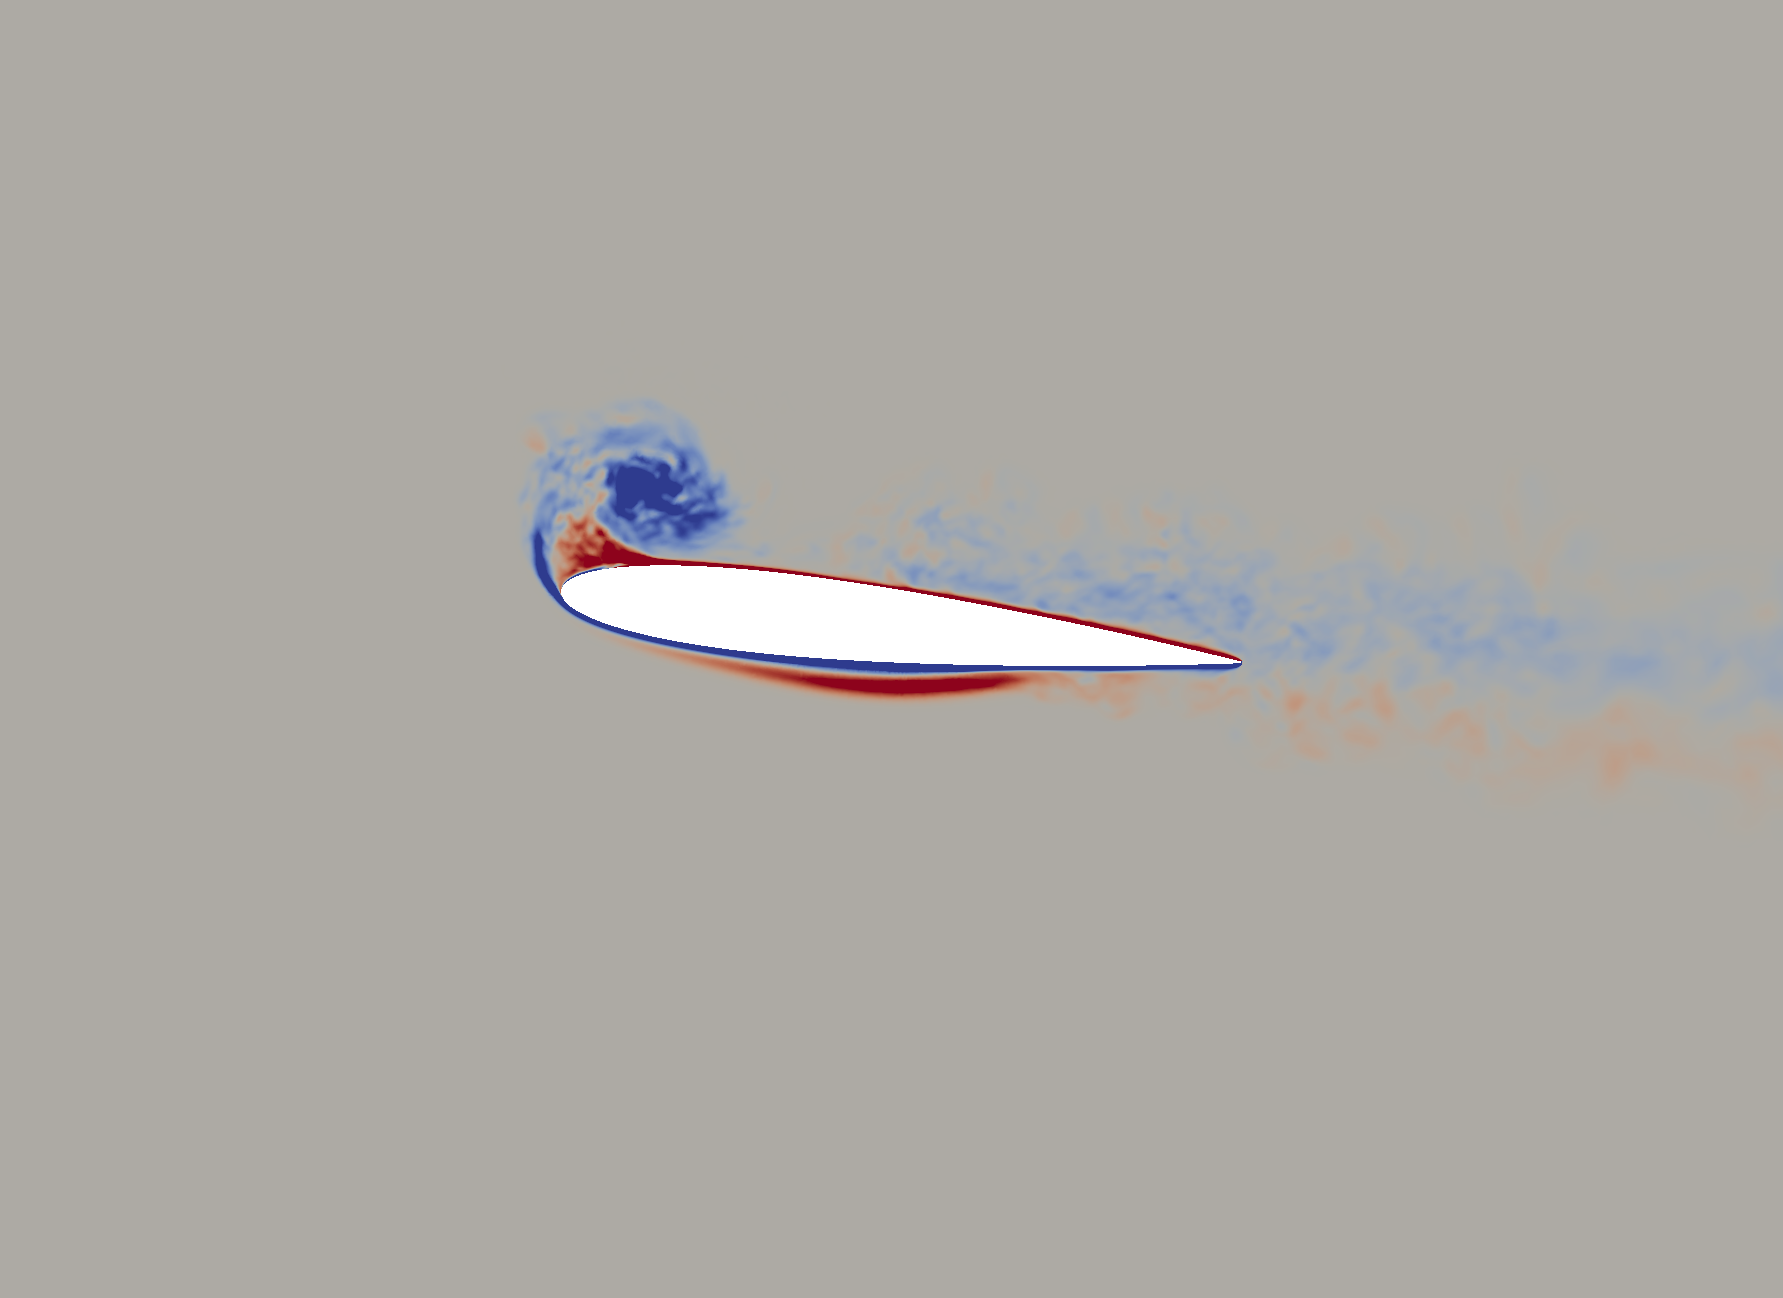
\includegraphics[width=1\textwidth]{figures/Vorticity_plots/Re_40k_1pt2/phase_240.png}
		\caption{$Re=4e4$, $\psi$ = $240^\circ$, $\tilde{t}=0.667$}
		\label{fig:Re_40k_1pt2_phi240}
	\end{subfigure}
	\begin{subfigure}[b]{0.32\textwidth}
		\centering
		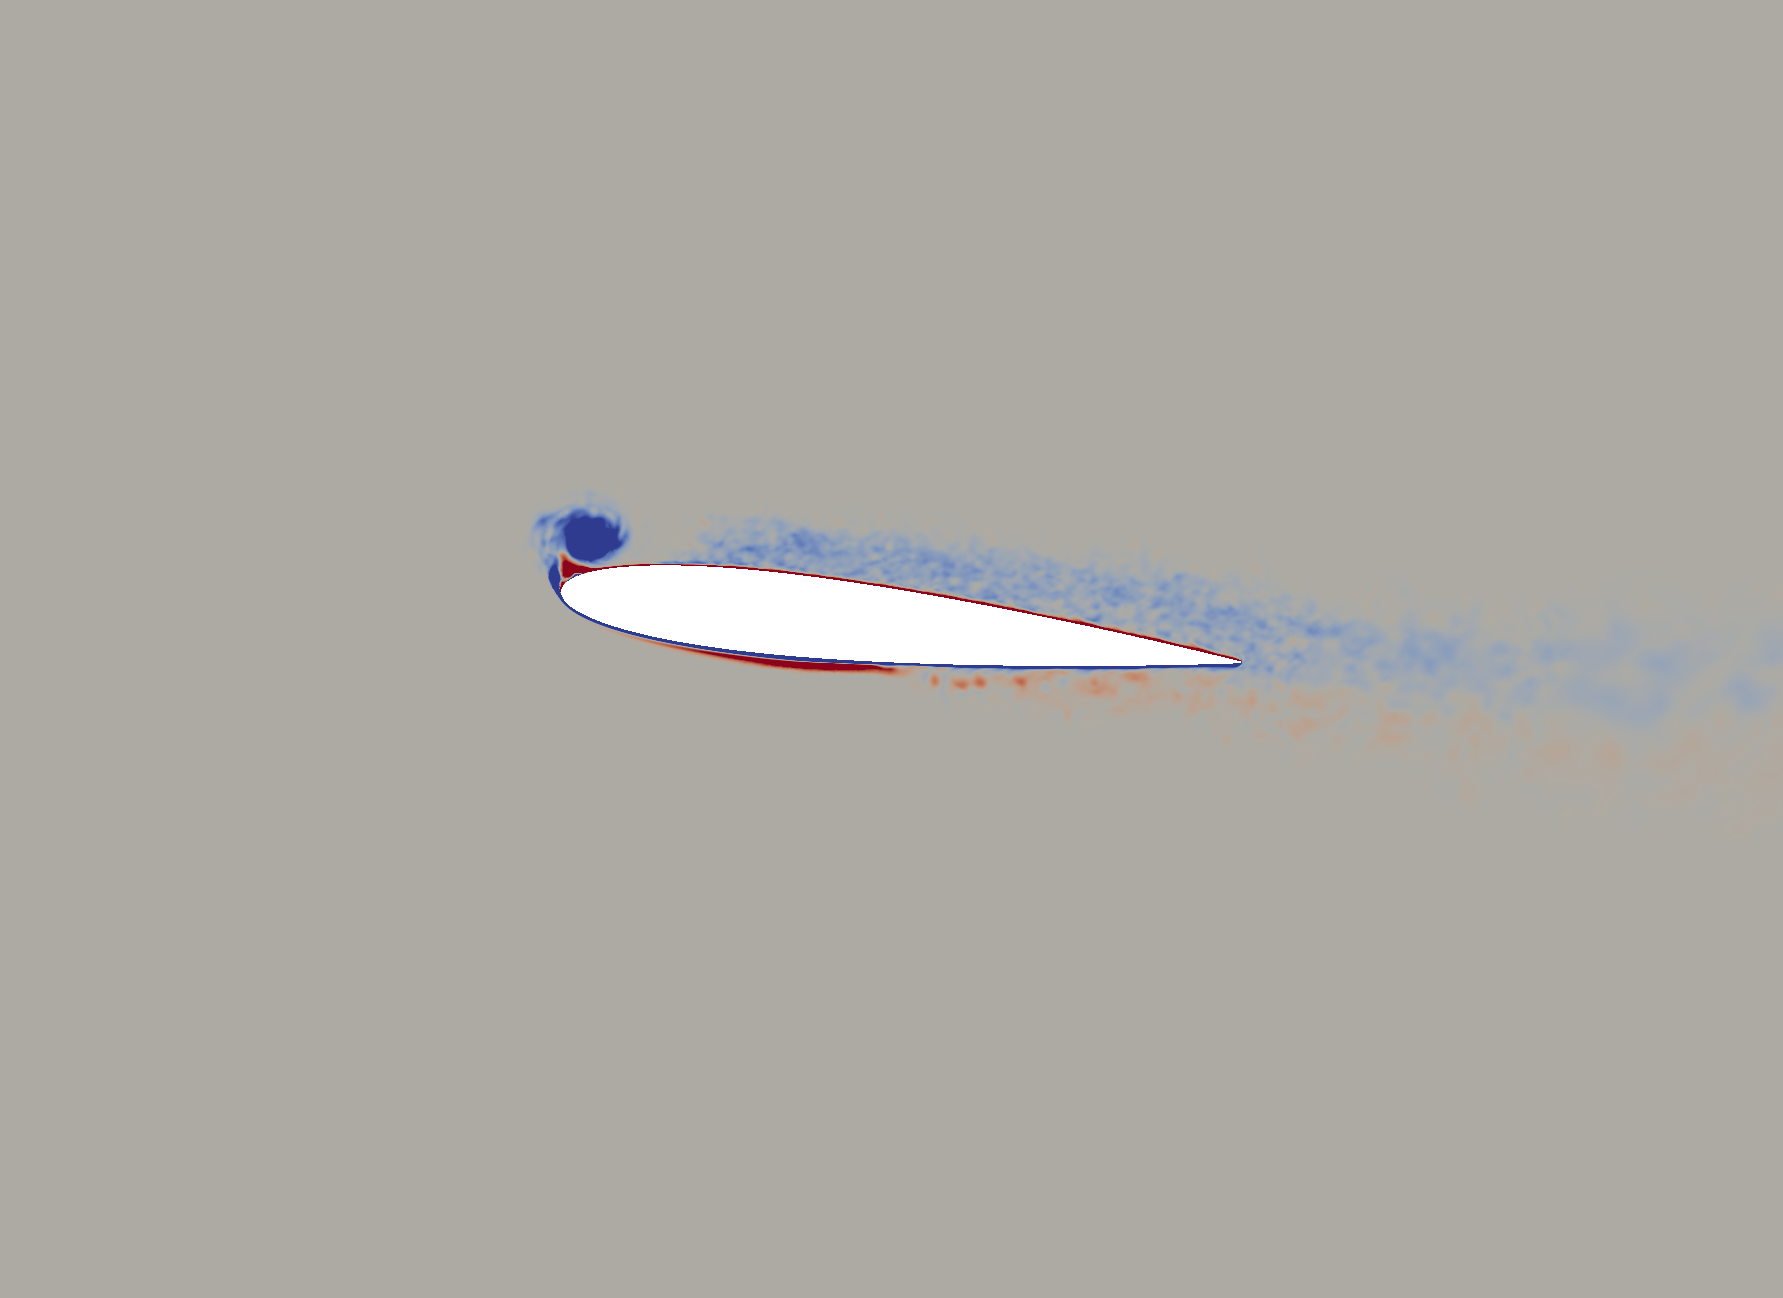
\includegraphics[width=1\textwidth]{figures/Vorticity_plots/Re_200k_1pt2/phase_240.png}
		\caption{$Re=2e5$, $\psi$ = $240^\circ$, $\tilde{t}=0.667$}
		\label{fig:Re_200k_1pt2_phi240}
	\end{subfigure}
	\begin{subfigure}[b]{0.32\textwidth}
		\centering
		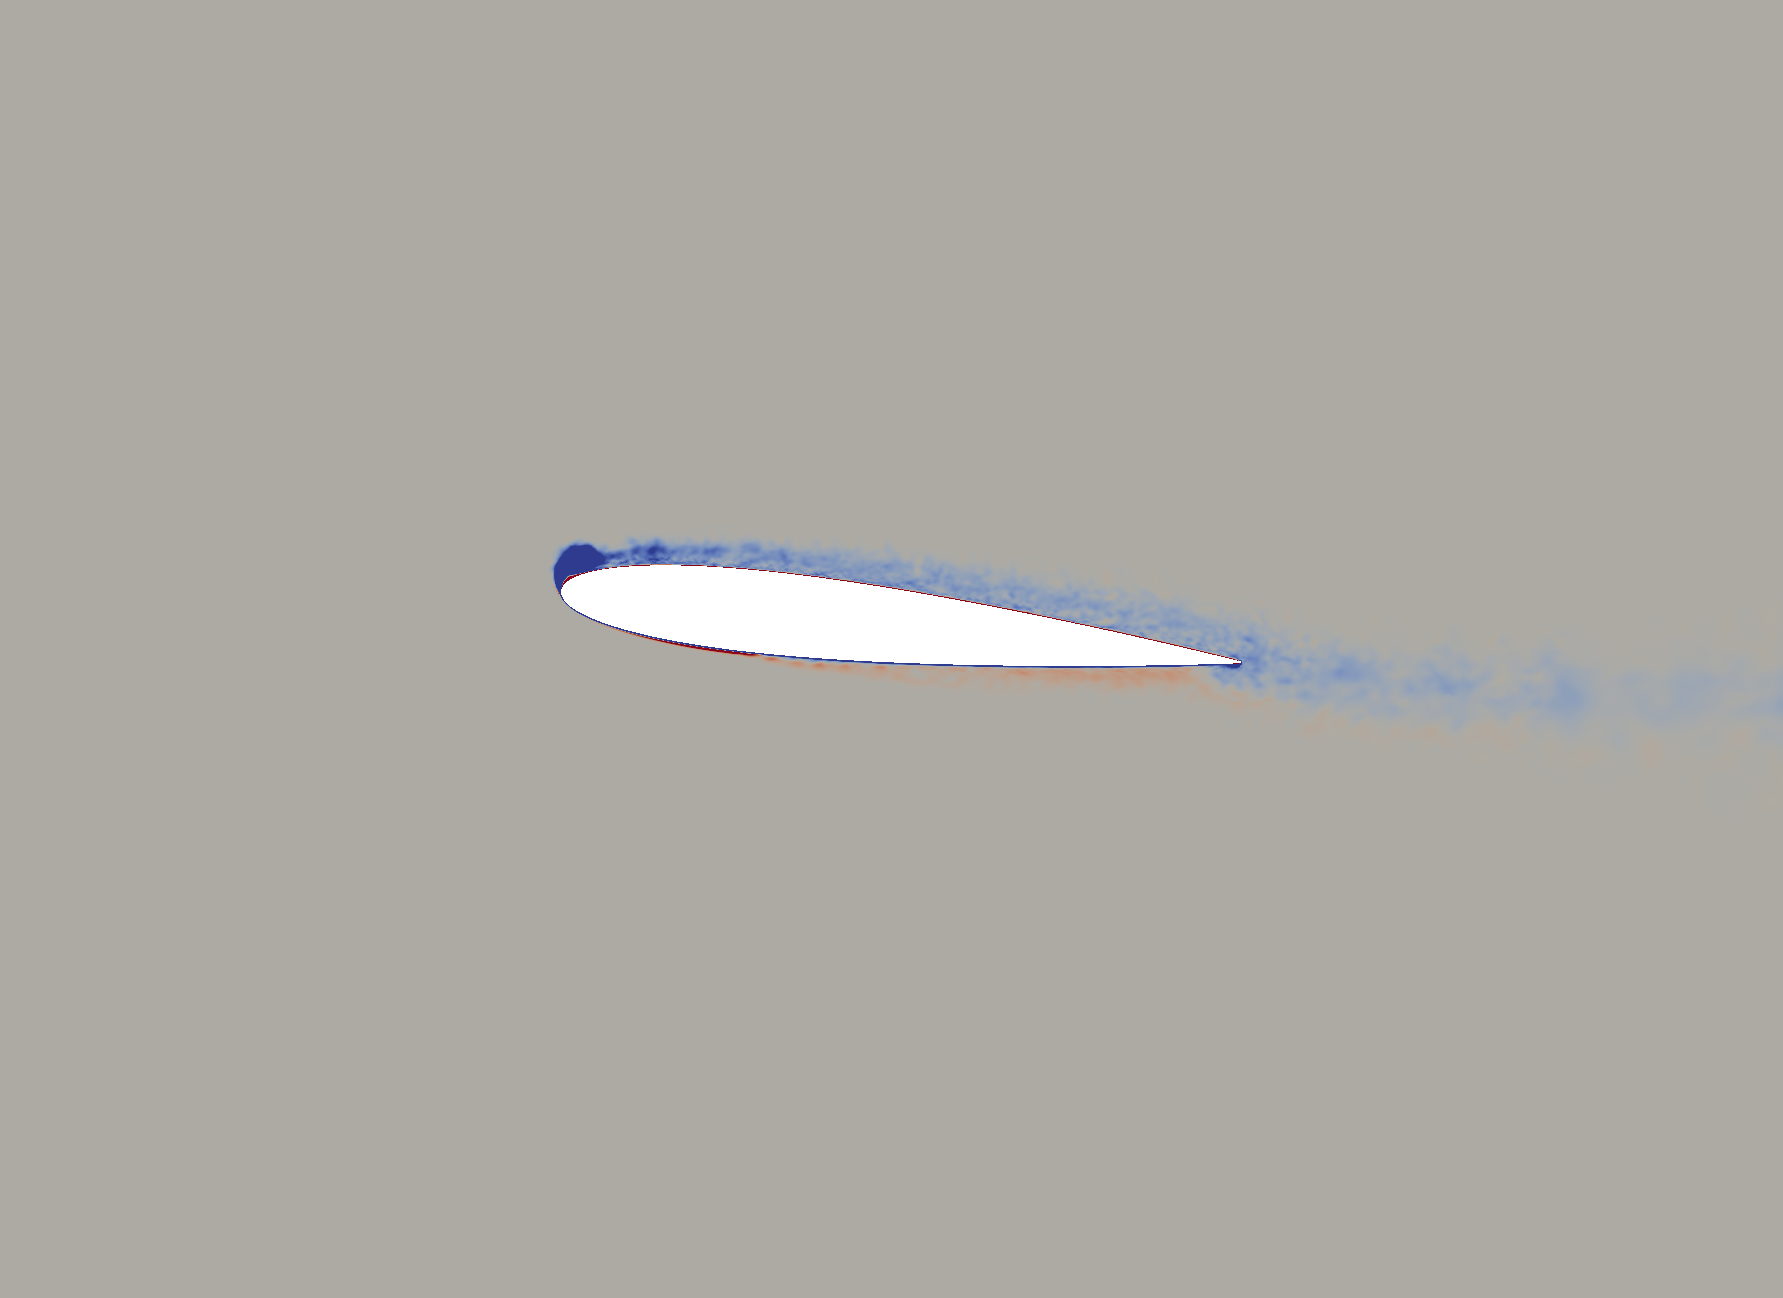
\includegraphics[width=1\textwidth]{figures/Vorticity_plots/Re_1m_1pt2/phase_240.png}
		\caption{$Re=1e6$, $\psi$ = $240^\circ$, $\tilde{t}=0.667$}
		\label{fig:Re_1m_1pt2_phi240}
	\end{subfigure}
	
	\begin{subfigure}[b]{0.32\textwidth}
		\centering
		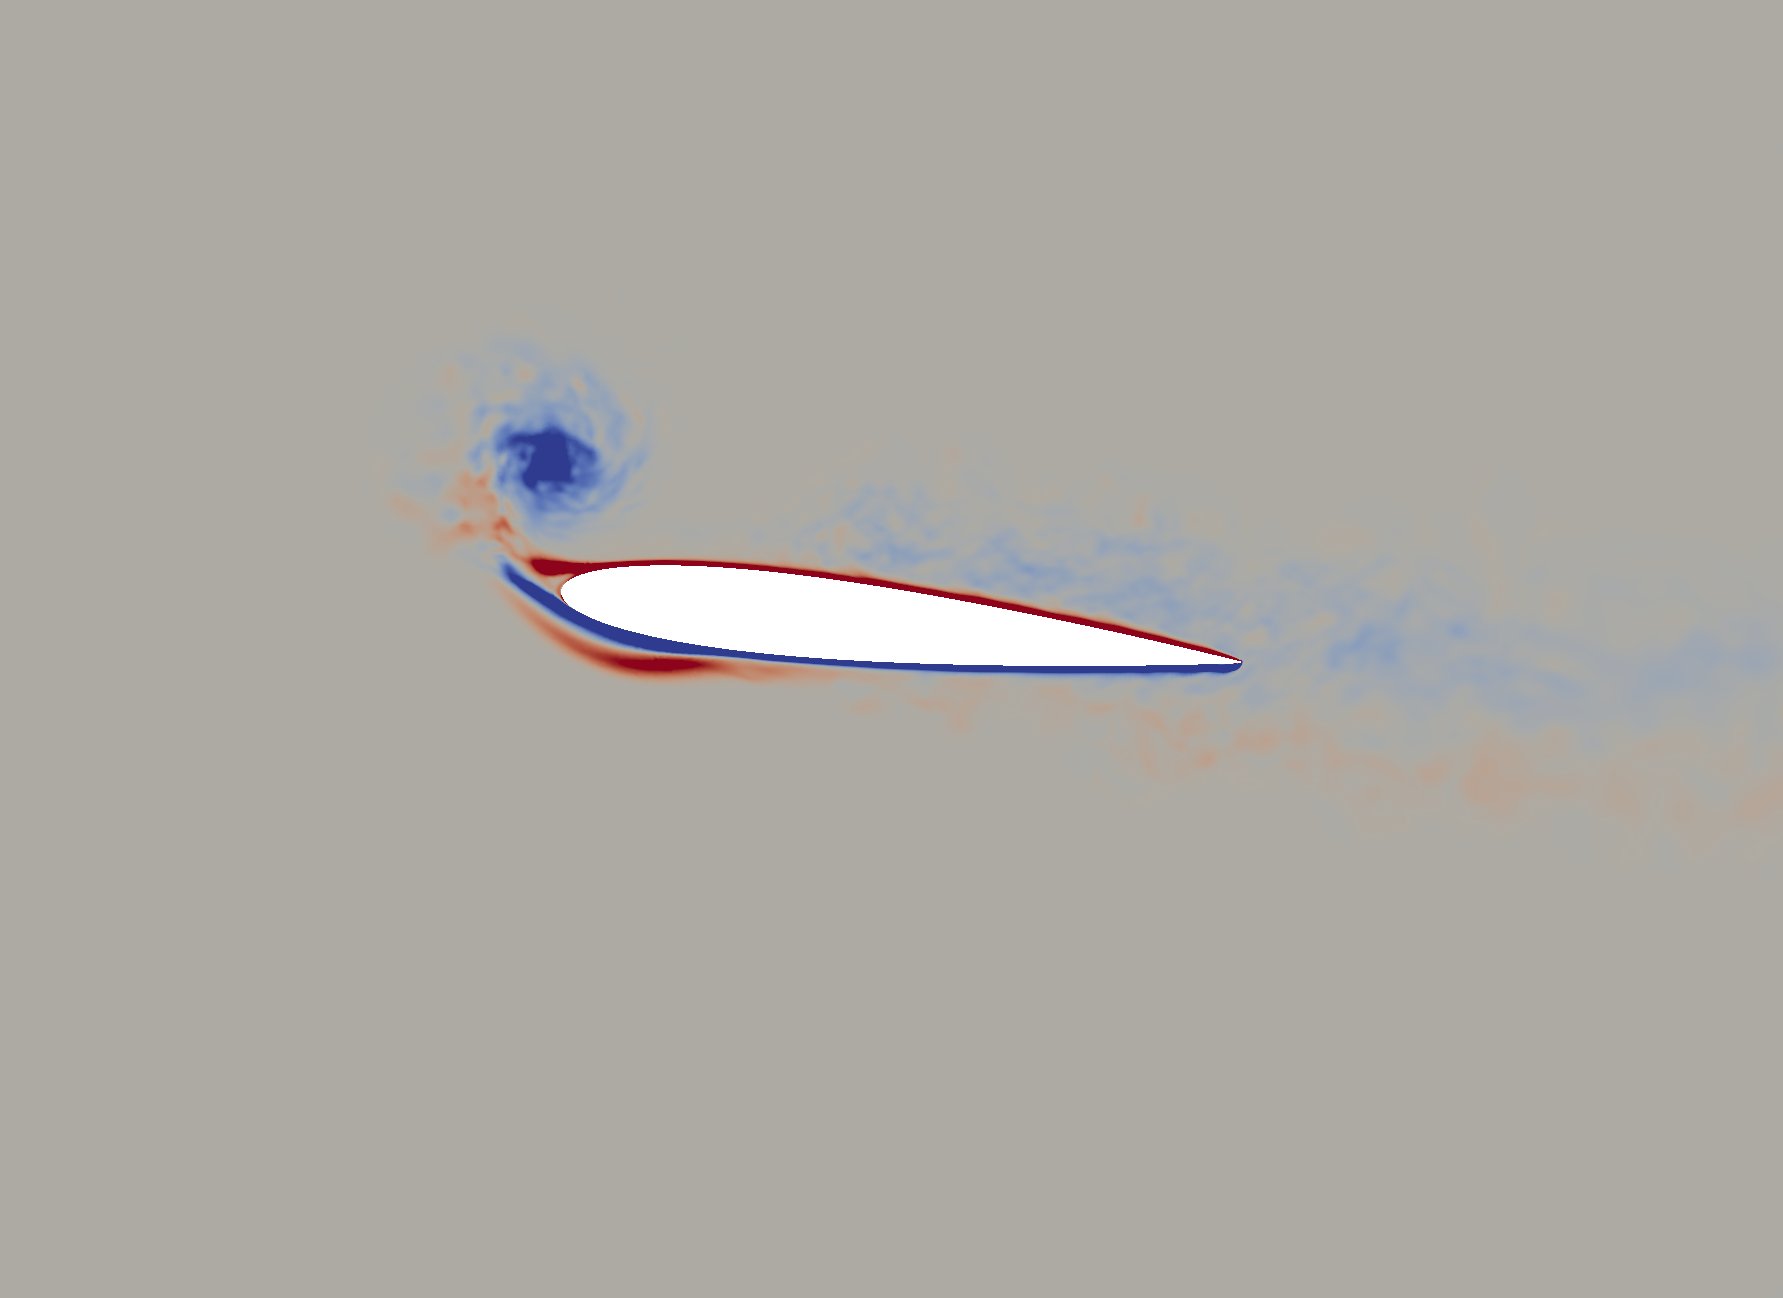
\includegraphics[width=1\textwidth]{figures/Vorticity_plots/Re_40k_1pt2/phase_255.png}
		\caption{$Re=4e4$, $\psi$ = $255^\circ$, $\tilde{t}=0.708$}
		\label{fig:Re_40k_1pt2_phi255}
	\end{subfigure}
	\begin{subfigure}[b]{0.32\textwidth}
		\centering
		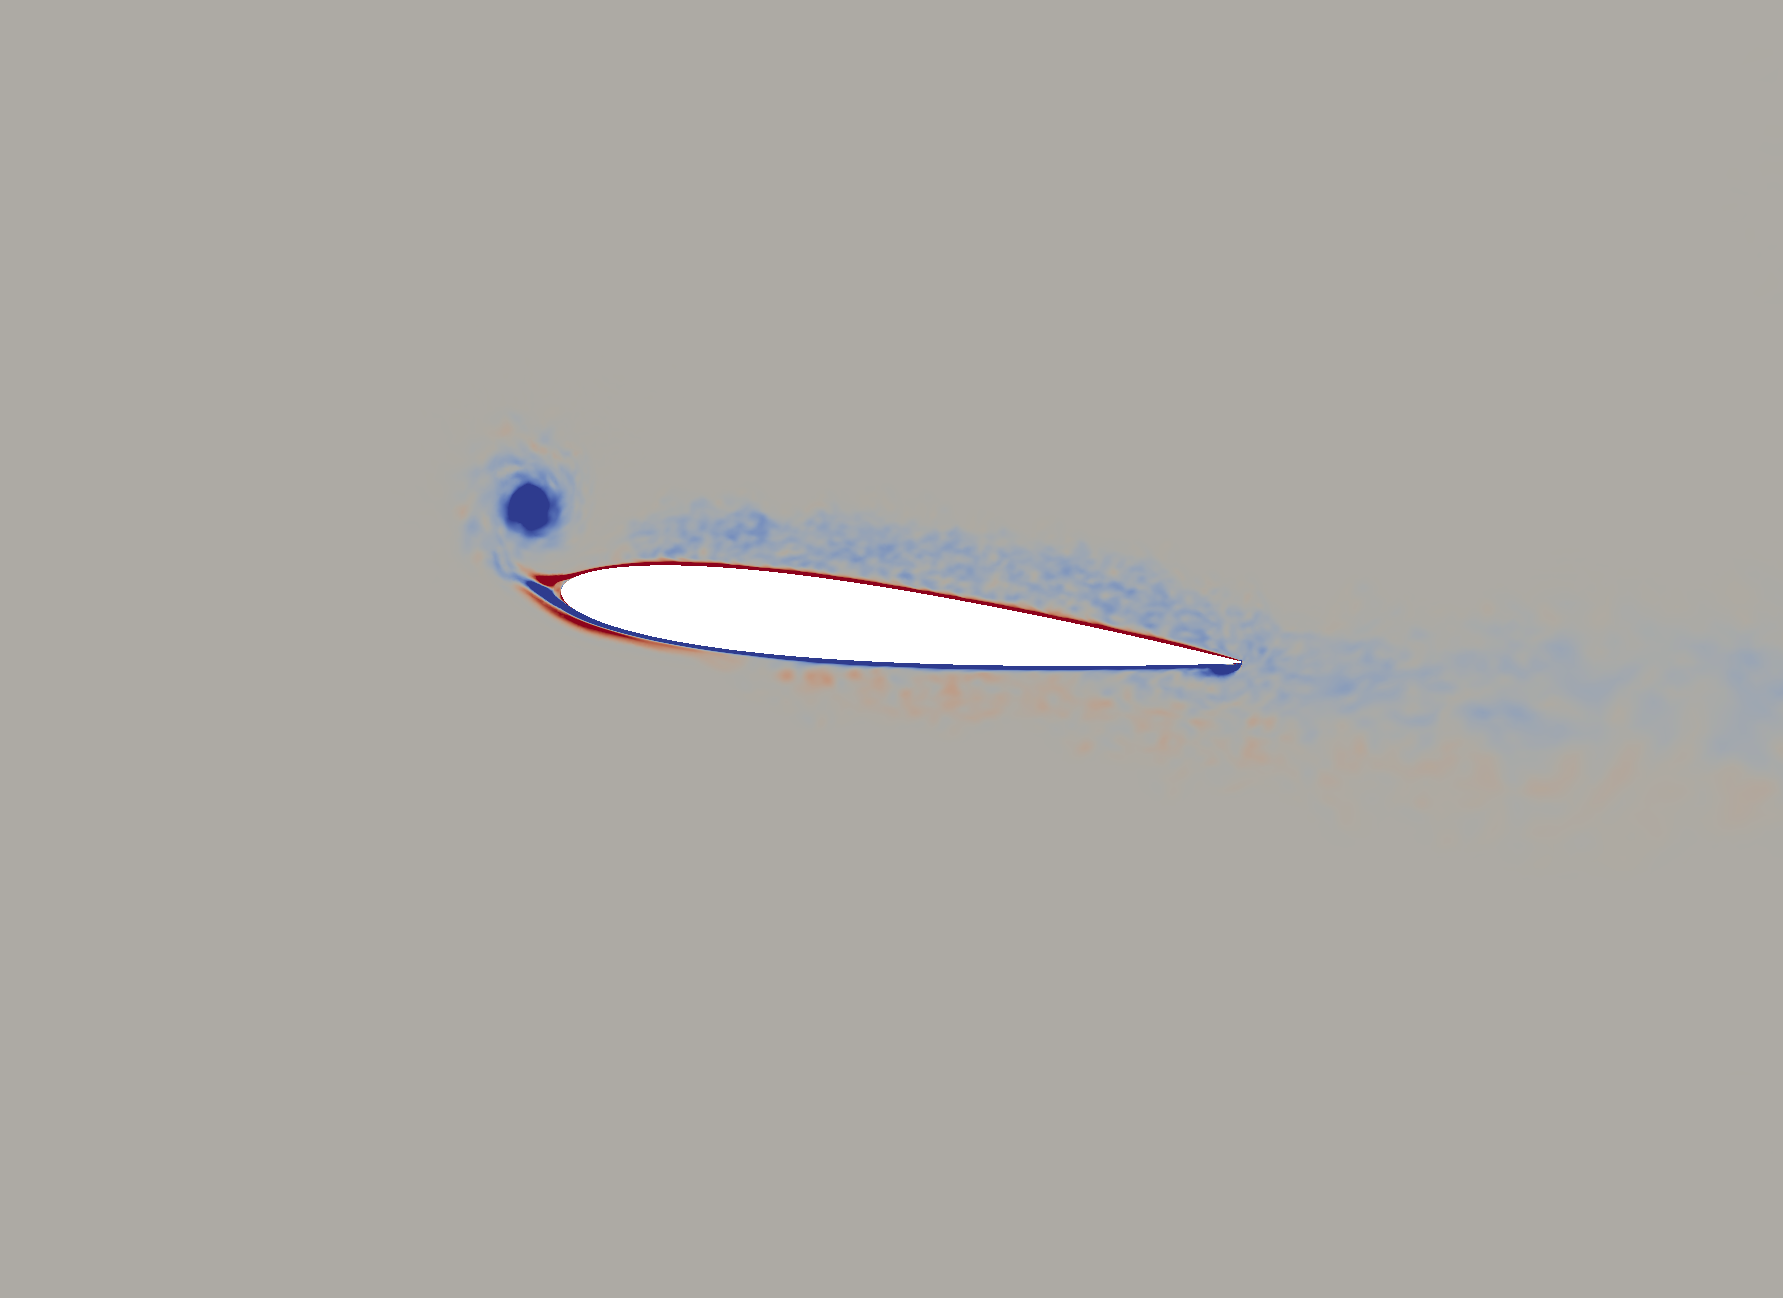
\includegraphics[width=1\textwidth]{figures/Vorticity_plots/Re_200k_1pt2/phase_255.png}
		\caption{$Re=2e5$, $\psi$ = $255^\circ$, $\tilde{t}=0.708$}
		\label{fig:Re_200k_1pt2_phi255}
	\end{subfigure}
	\begin{subfigure}[b]{0.32\textwidth}
		\centering
		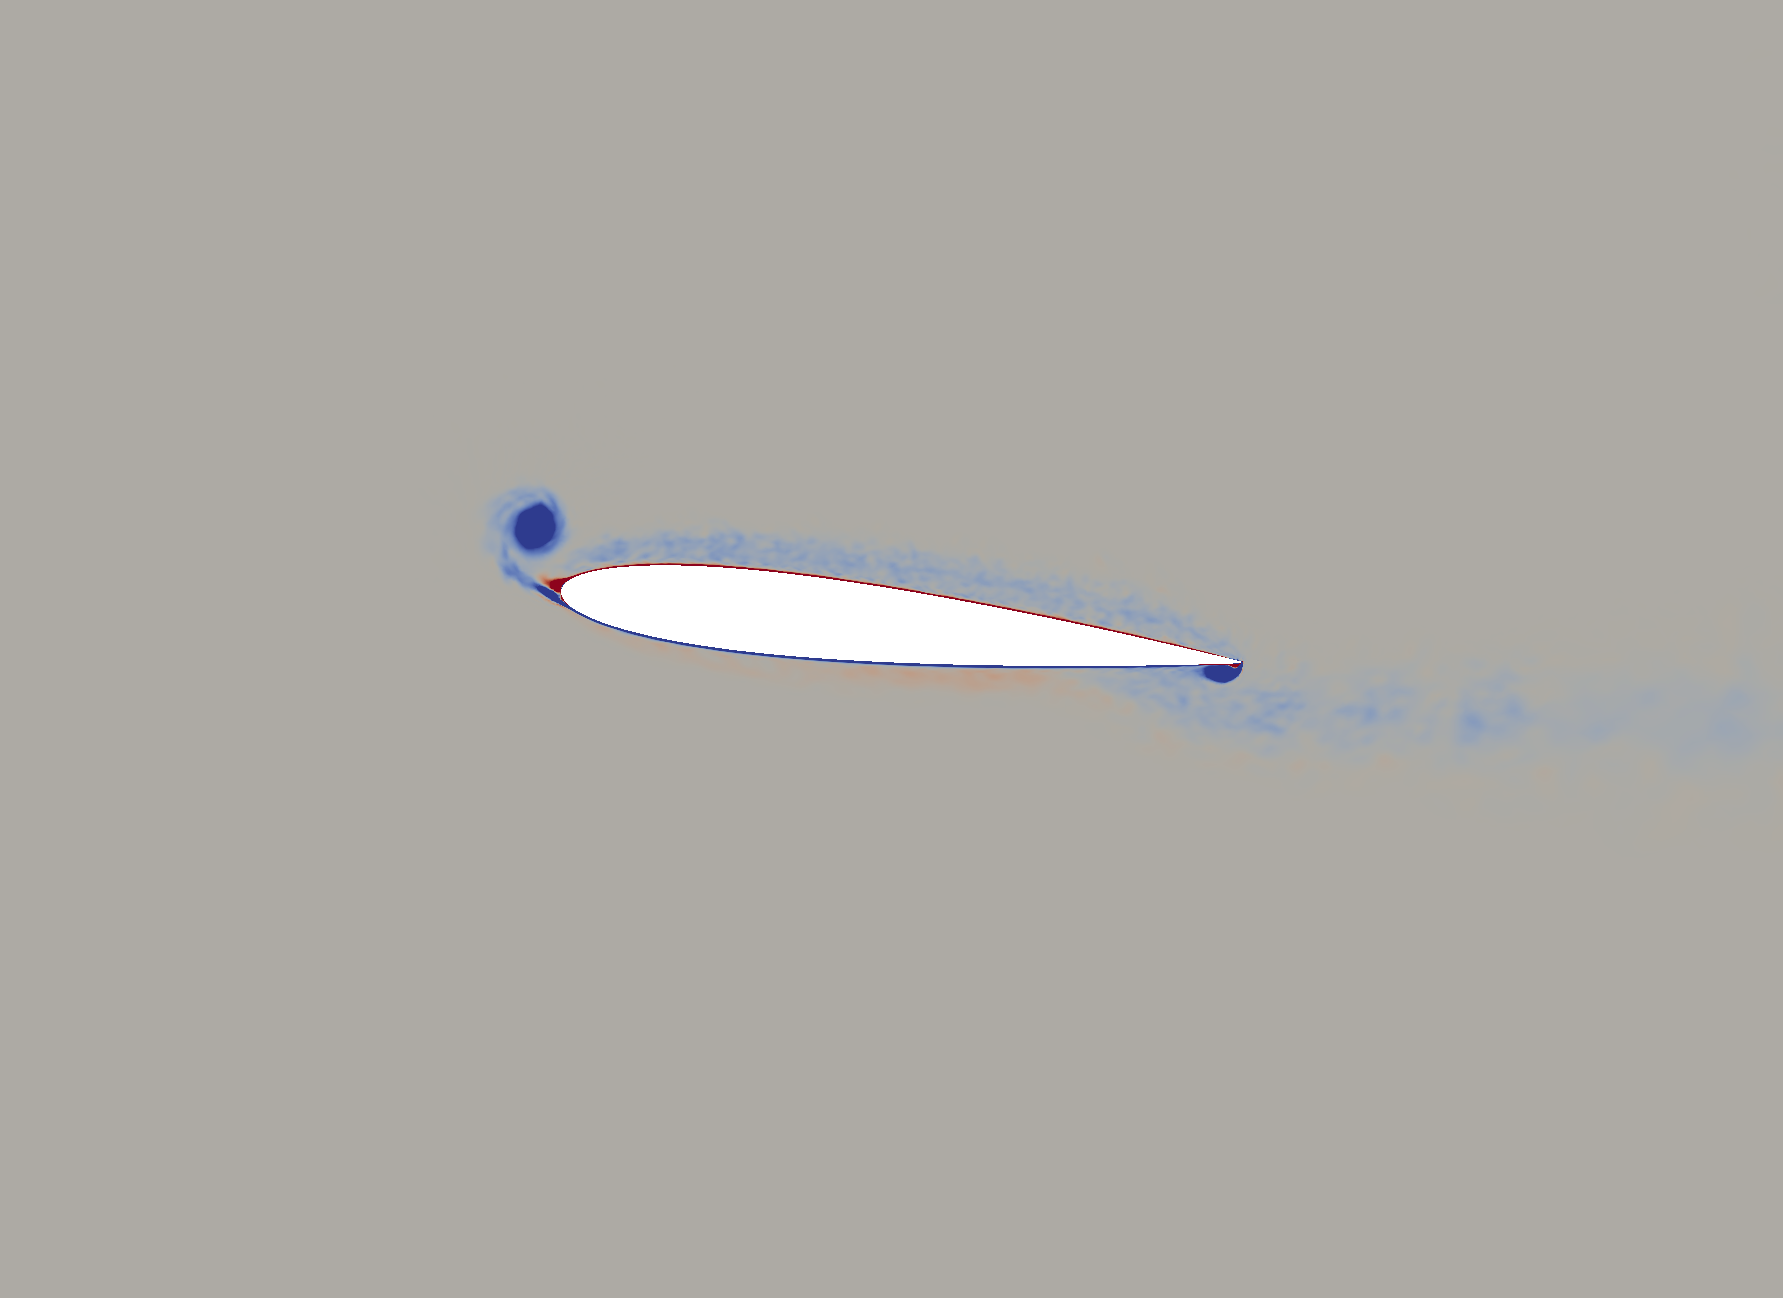
\includegraphics[width=1\textwidth]{figures/Vorticity_plots/Re_1m_1pt2/phase_255.png}
		\caption{$Re=1e6$, $\psi$ = $255^\circ$, $\tilde{t}=0.708$}
		\label{fig:Re_1m_1pt2_phi255}
	\end{subfigure}
	
	\caption{Spanwise vorticity at 8 different phases for $Re$=40,000 (left column), 200,000 (middle column) and 1,000,000 (right column) at $\mu_{sect}$ = 1.2}
%	\label{fig:vortScreen_1pt2}
\end{figure}


\begin{figure}[H]\ContinuedFloat
	\centering
	\begin{subfigure}[b]{0.32\textwidth}
		\centering
		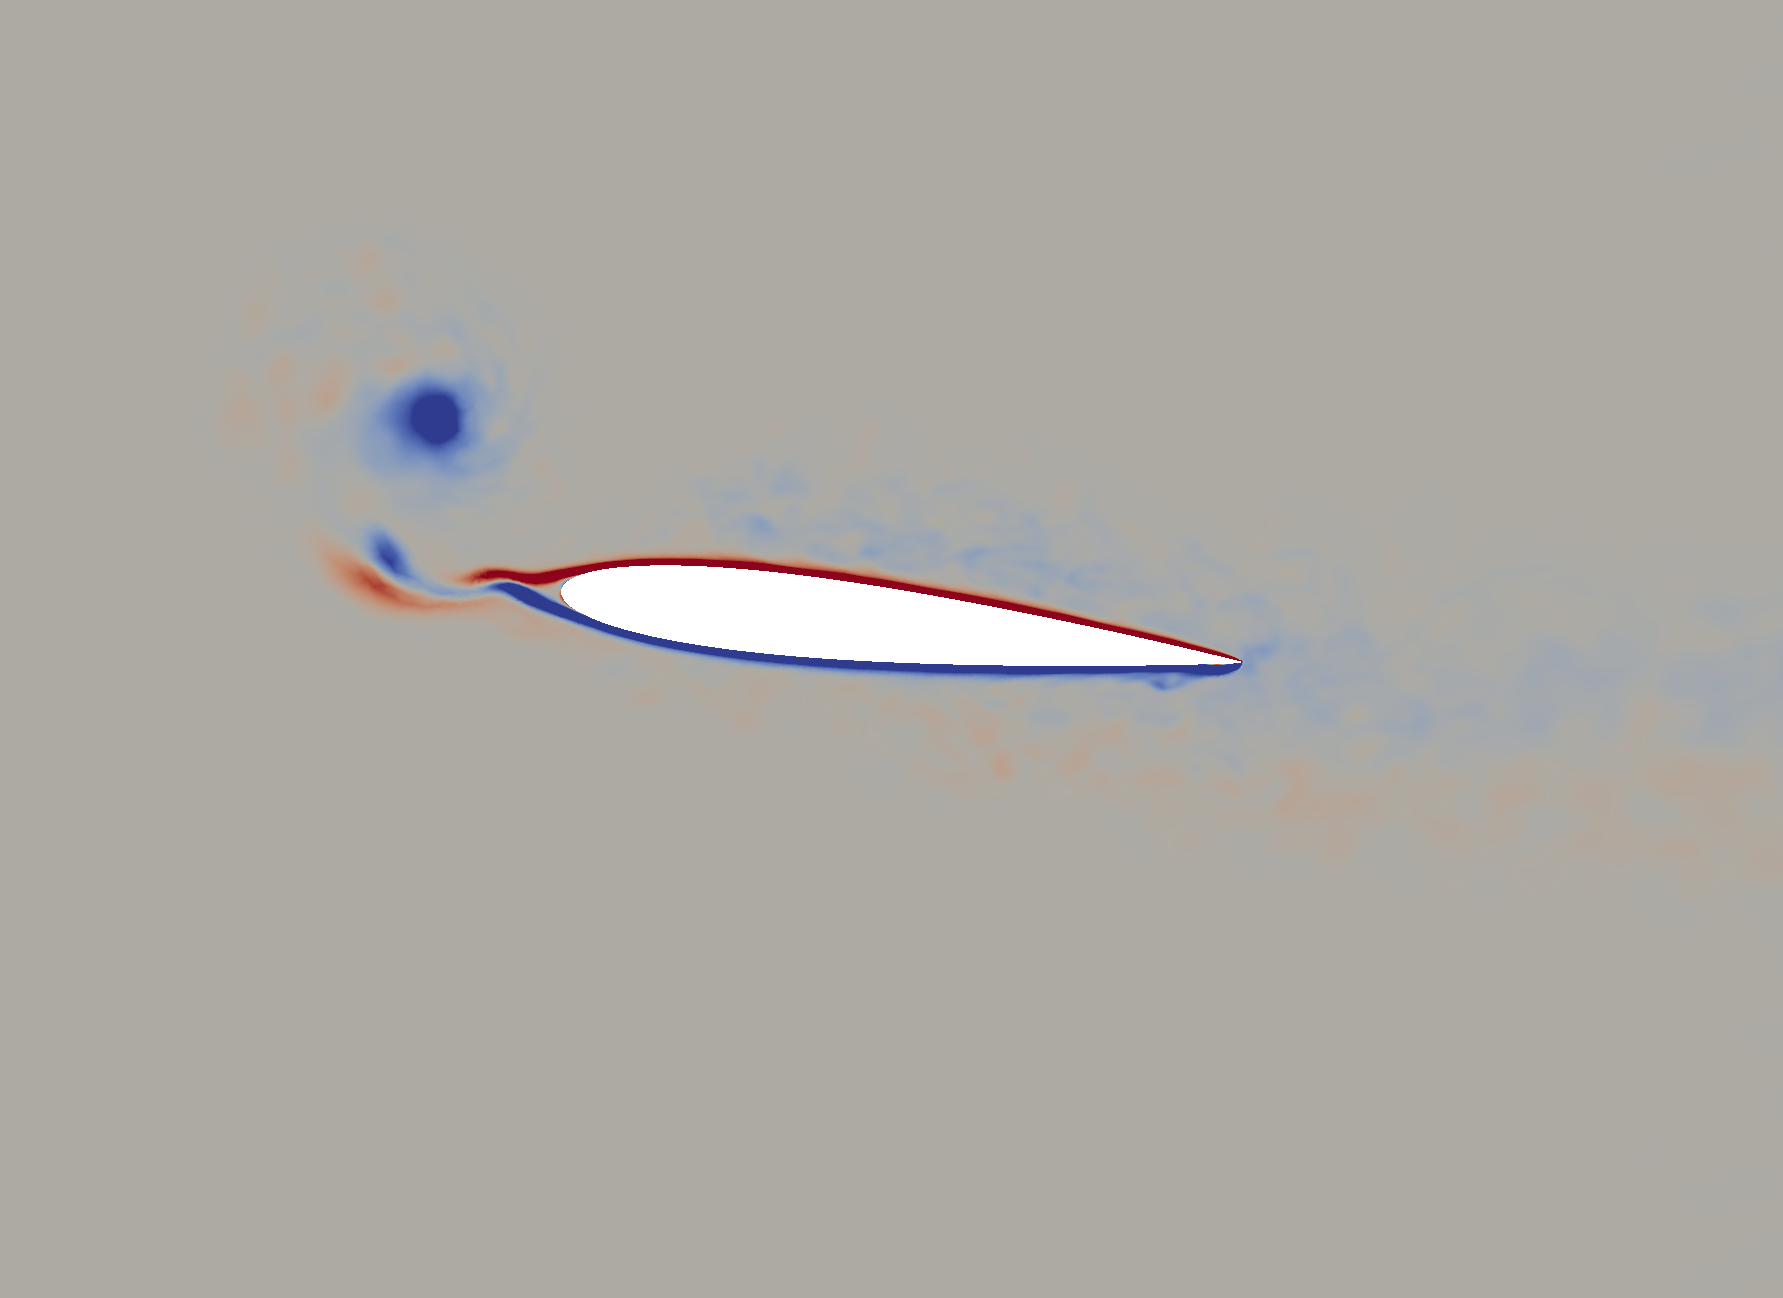
\includegraphics[width=1\textwidth]{figures/Vorticity_plots/Re_40k_1pt2/phase_270.png}
		\caption{$Re=4e4$, $\psi$ = $270^\circ$, $\tilde{t}=0.750$}
		\label{fig:Re_40k_1pt2_phi270}
	\end{subfigure}
	\begin{subfigure}[b]{0.32\textwidth}
		\centering
		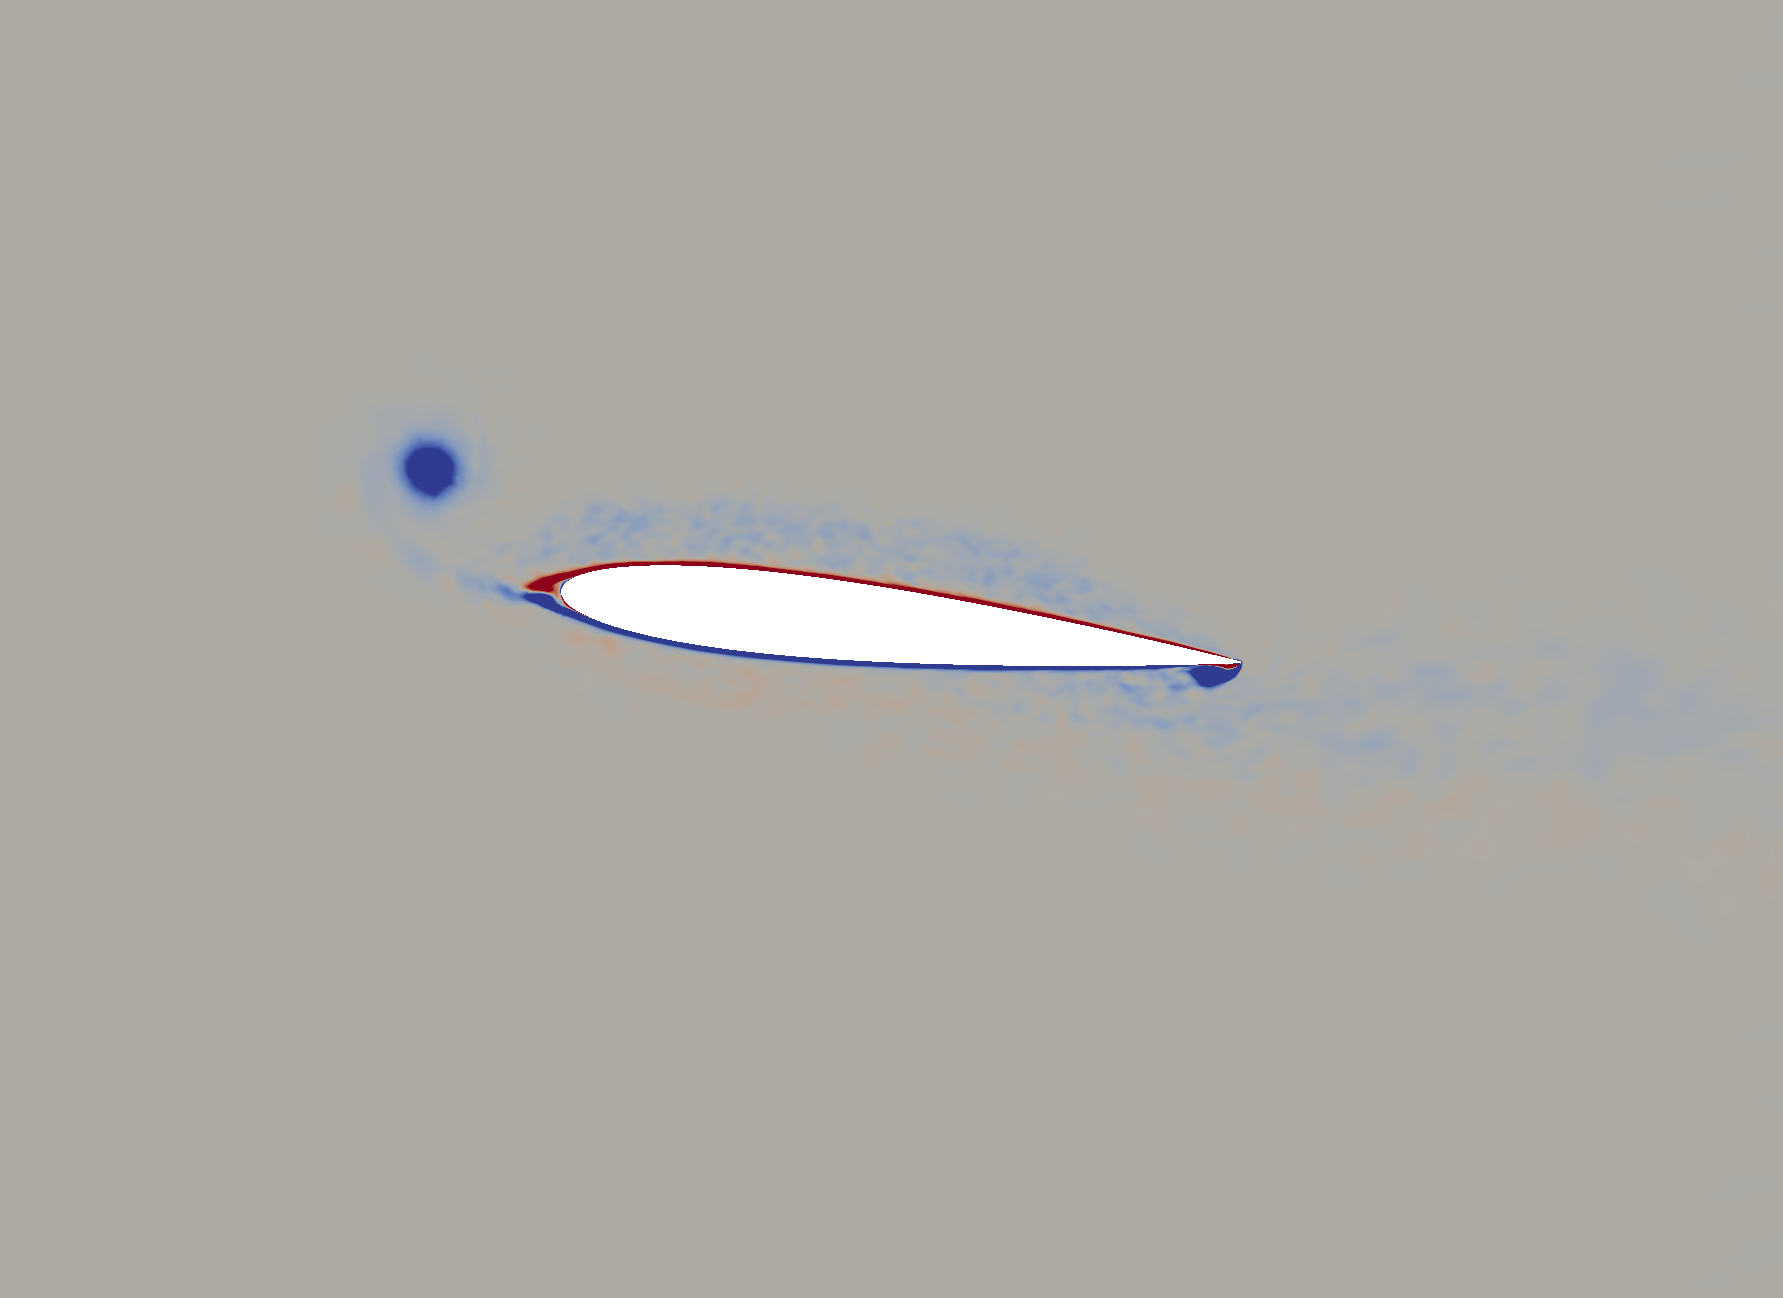
\includegraphics[width=1\textwidth]{figures/Vorticity_plots/Re_200k_1pt2/phase_270.png}
		\caption{$Re=2e5$, $\psi$ = $270^\circ$, $\tilde{t}=0.750$}
		\label{fig:Re_200k_1pt2_phi270}
	\end{subfigure}
	\begin{subfigure}[b]{0.32\textwidth}
		\centering
		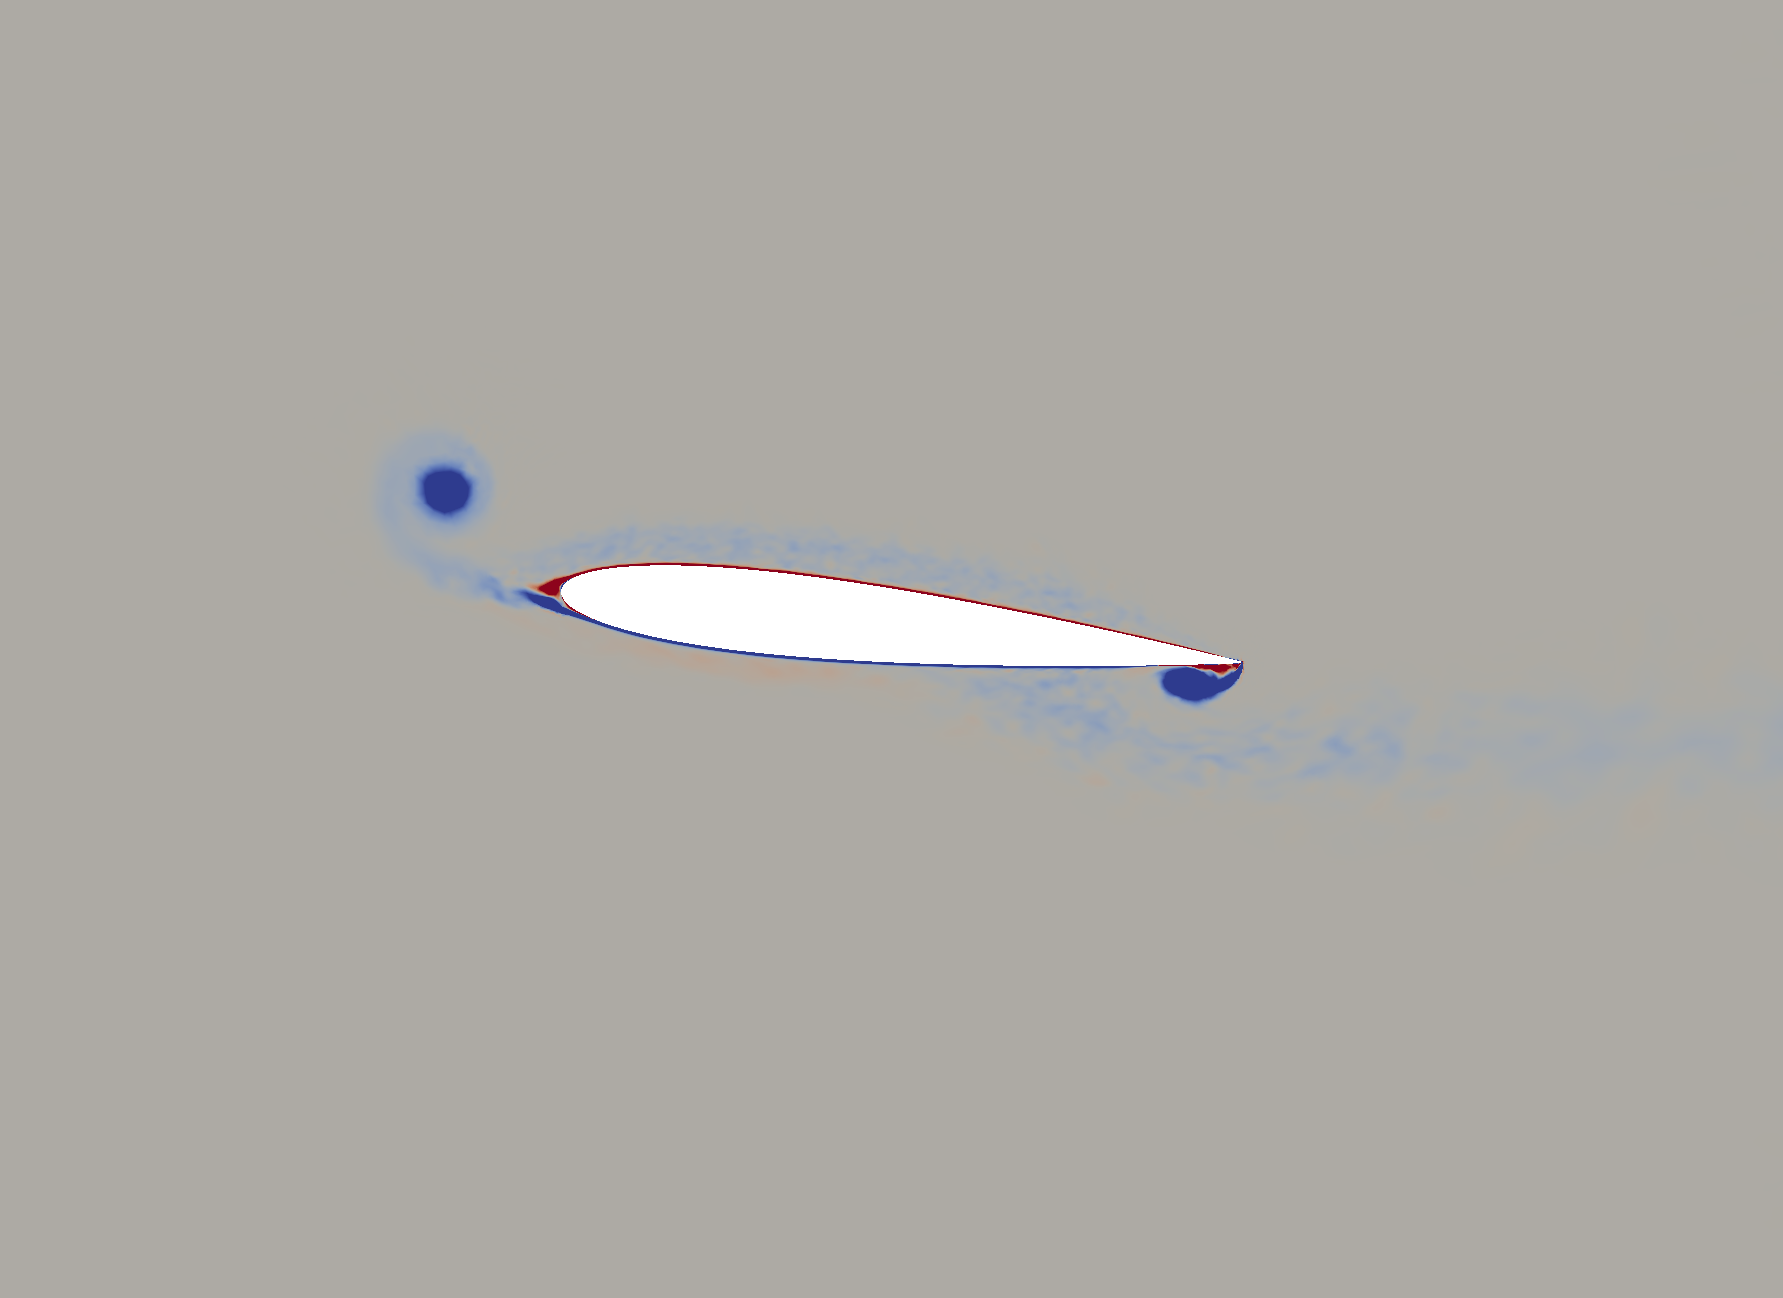
\includegraphics[width=1\textwidth]{figures/Vorticity_plots/Re_1m_1pt2/phase_270.png}
		\caption{$Re=1e6$, $\psi$ = $270^\circ$, $\tilde{t}=0.750$}
		\label{fig:Re_1m_1pt2_phi270}
	\end{subfigure}
	
	\begin{subfigure}[b]{0.32\textwidth}
		\centering
		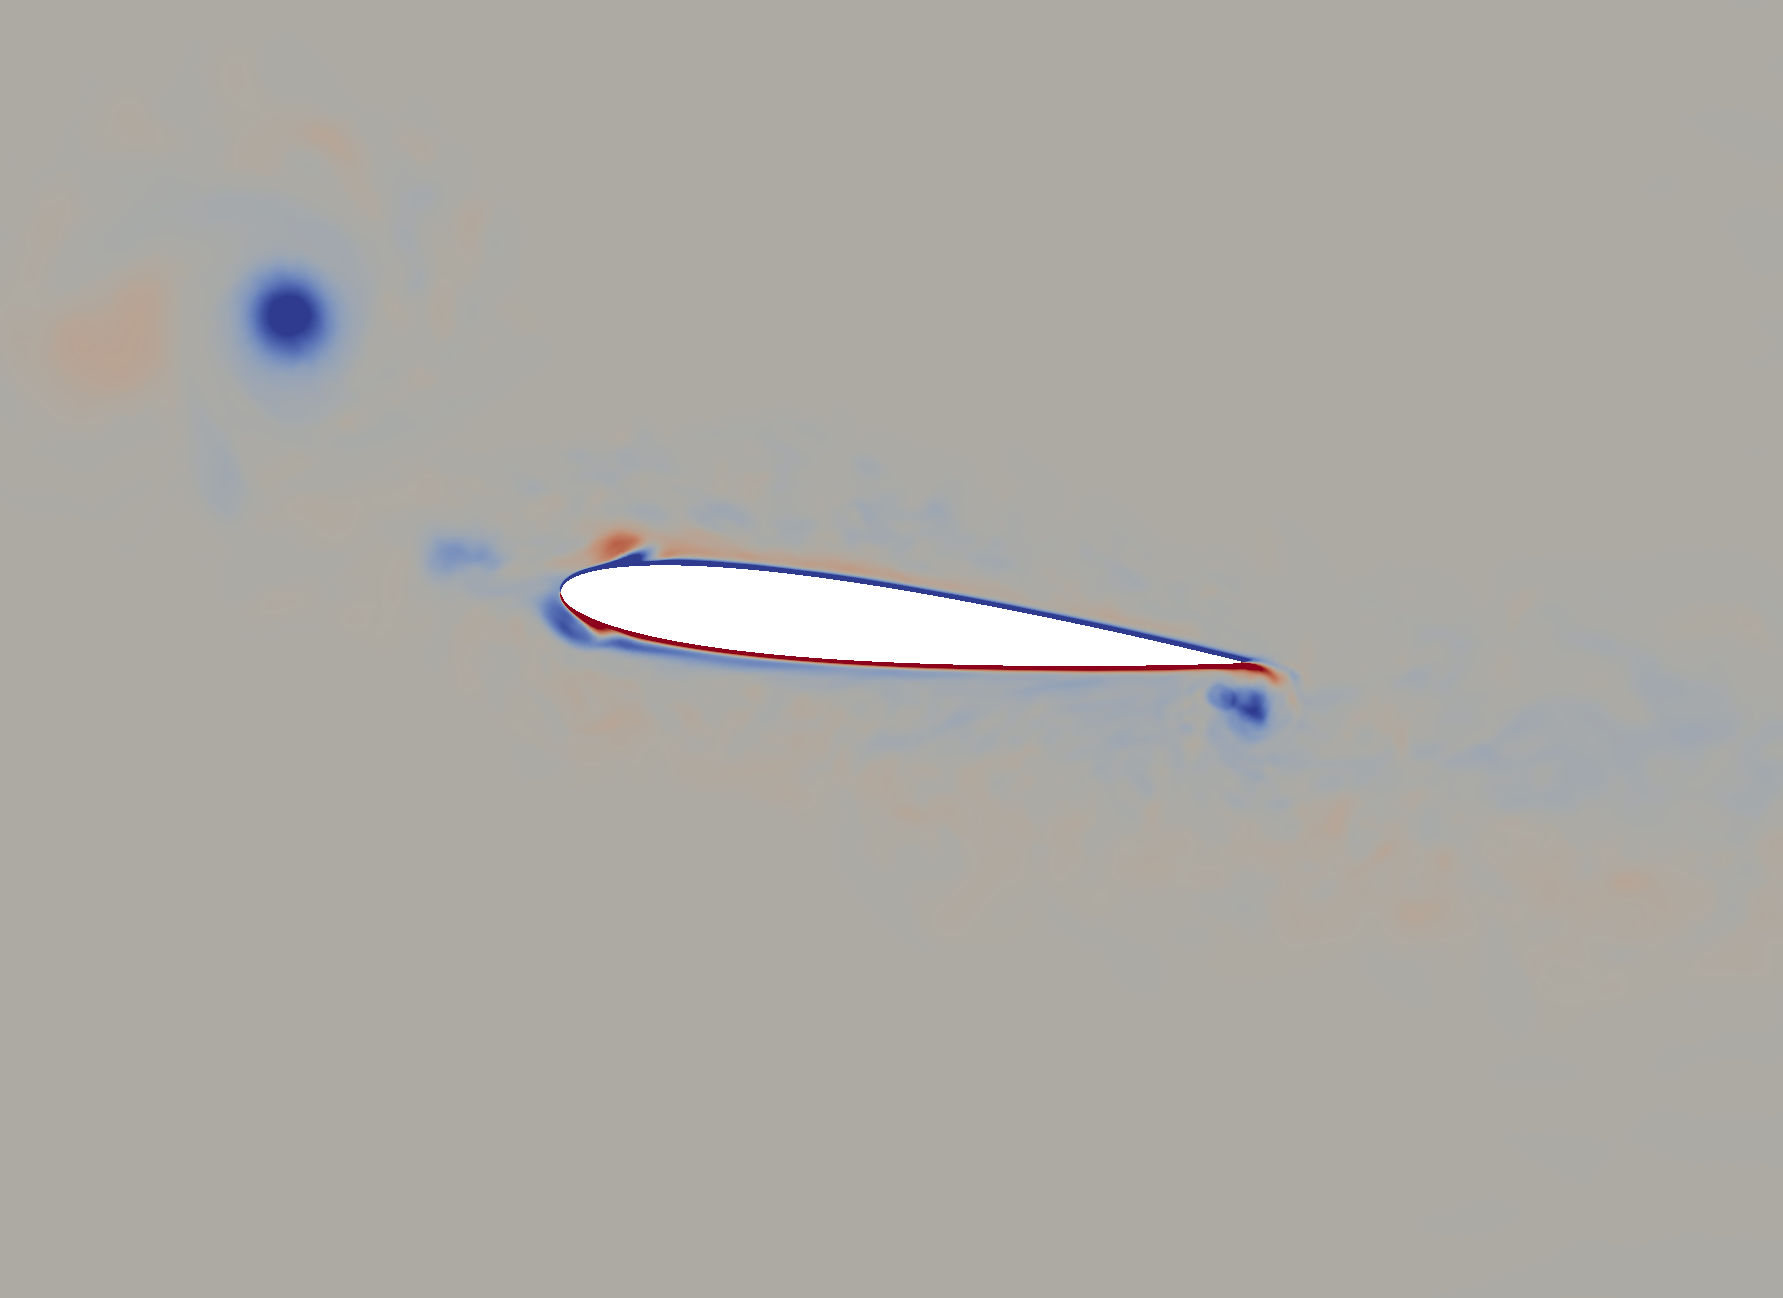
\includegraphics[width=1\textwidth]{figures/Vorticity_plots/Re_40k_1pt2/phase_315.png}
		\caption{$Re=4e4$, $\psi$ = $315^\circ$, $\tilde{t}=0.875$}
		\label{fig:Re_40k_1pt2_phi315}
	\end{subfigure}
	\begin{subfigure}[b]{0.32\textwidth}
		\centering
		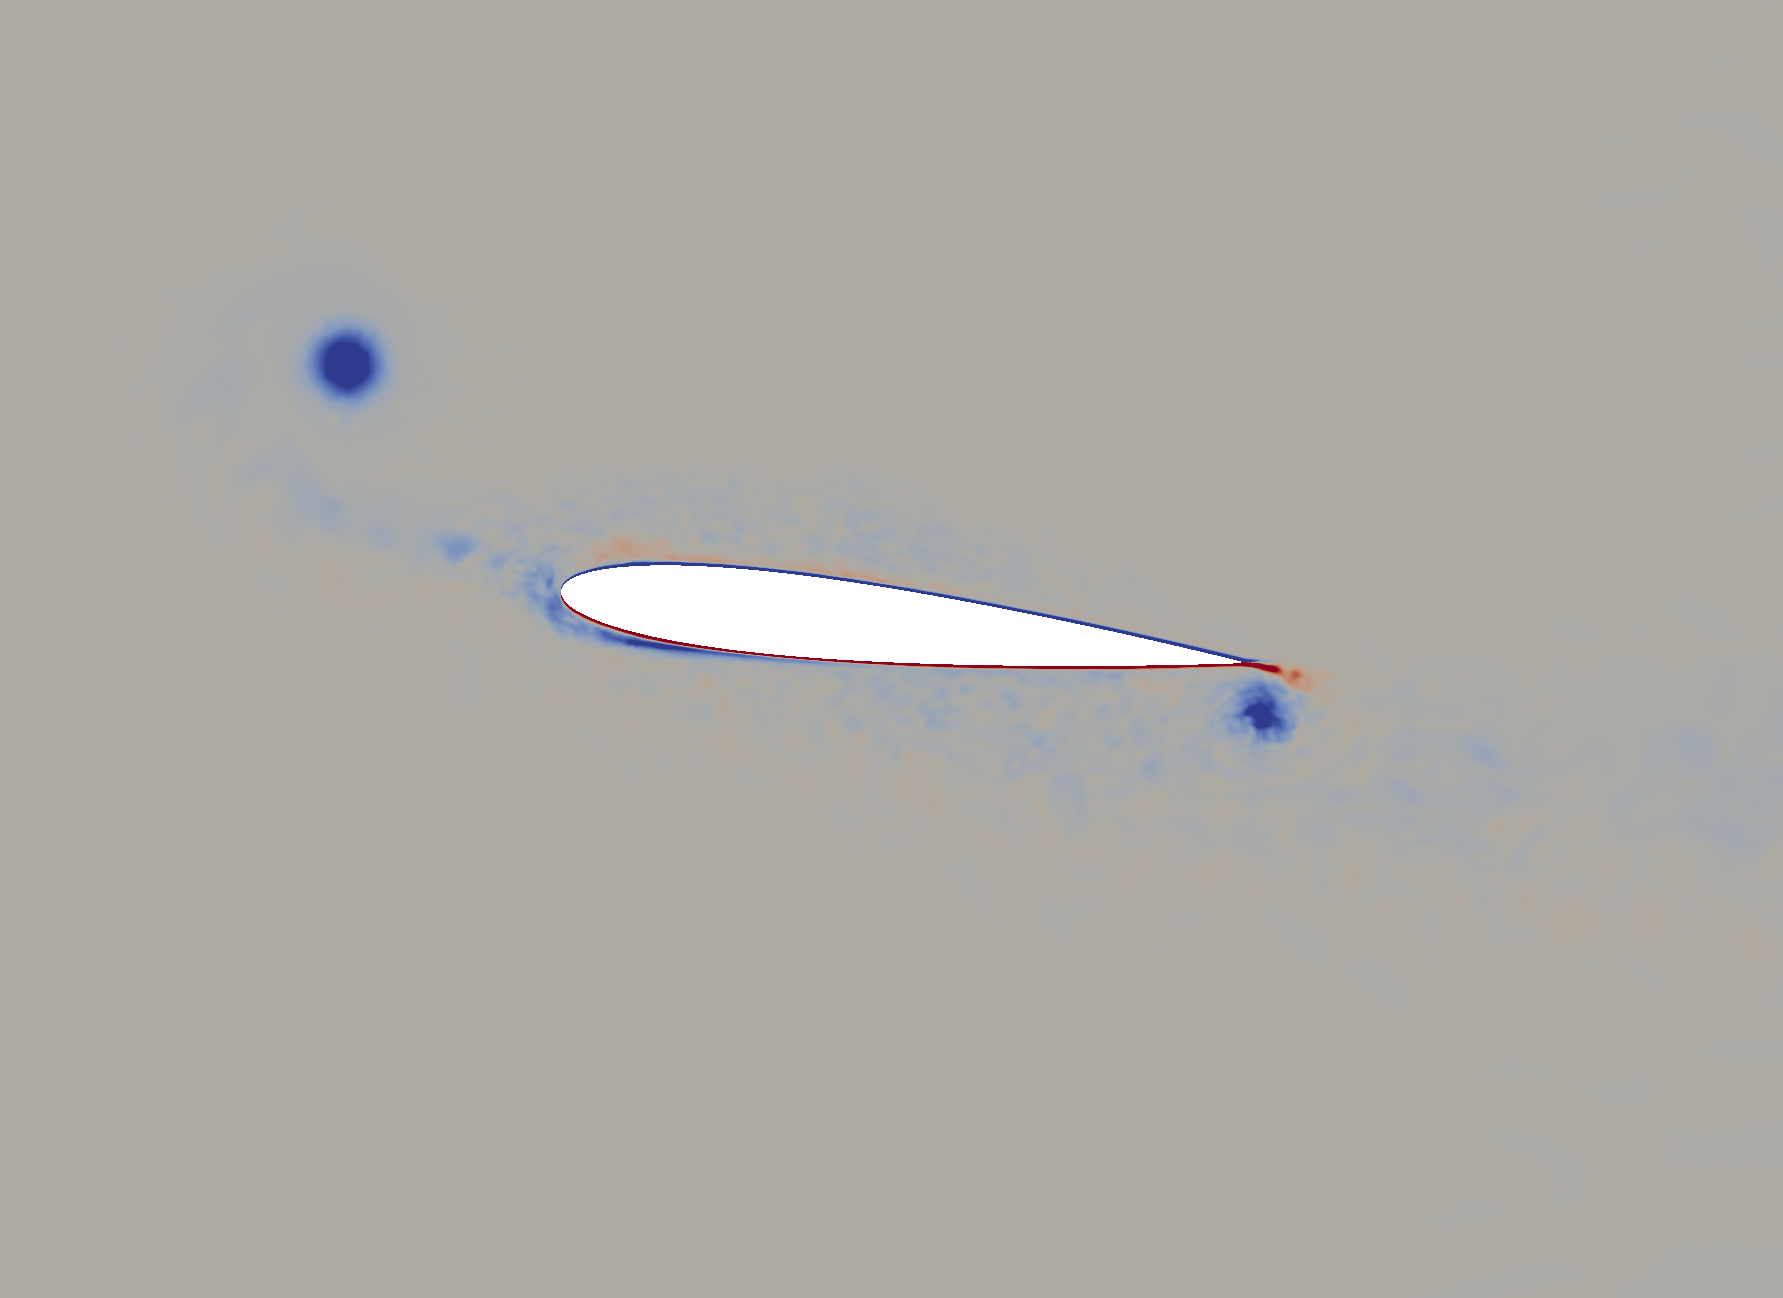
\includegraphics[width=1\textwidth]{figures/Vorticity_plots/Re_200k_1pt2/phase_315.png}
		\caption{$Re=2e5$, $\psi$ = $315^\circ$, $\tilde{t}=0.875$}
		\label{fig:Re_200k_1pt2_phi315}
	\end{subfigure}
	\begin{subfigure}[b]{0.32\textwidth}
		\centering
		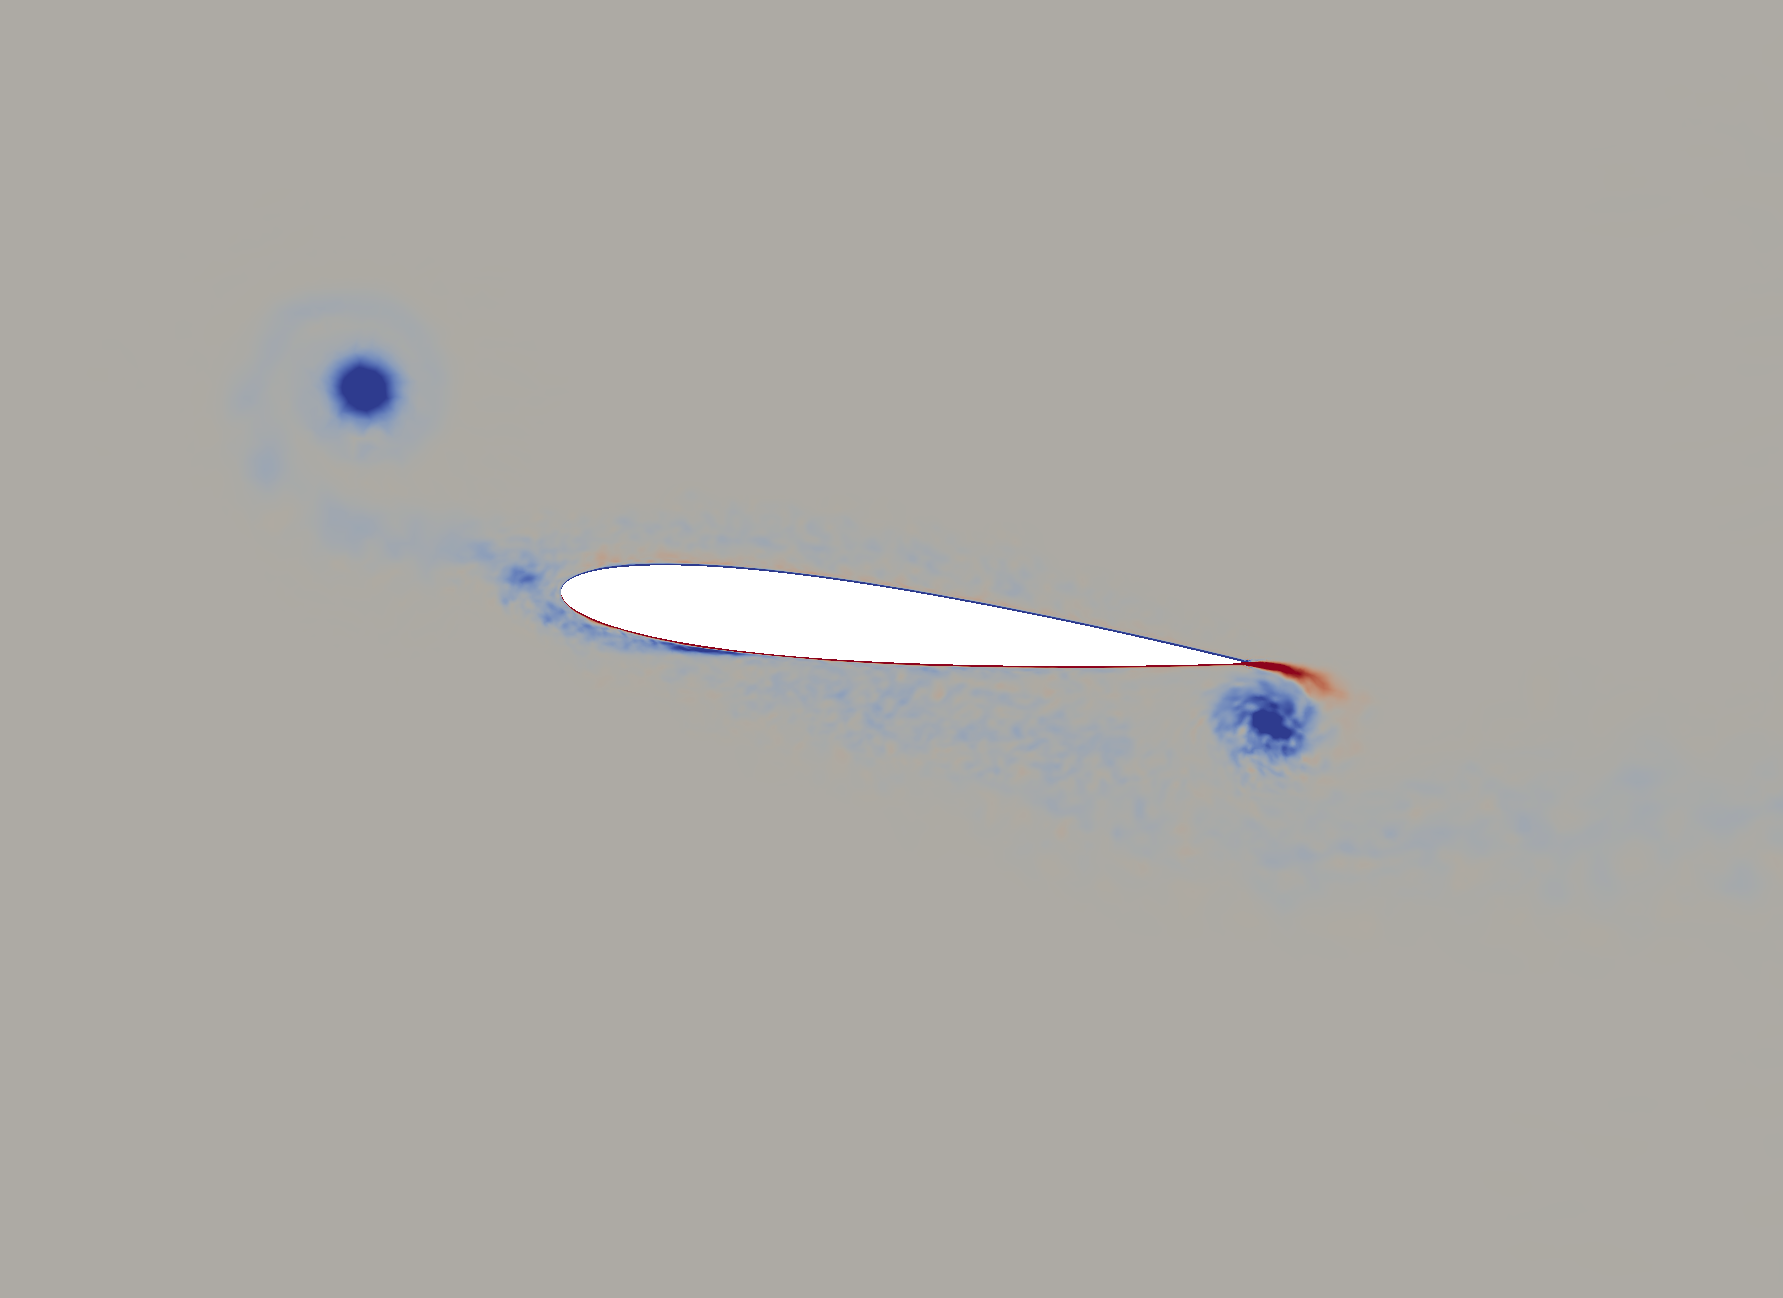
\includegraphics[width=1\textwidth]{figures/Vorticity_plots/Re_1m_1pt2/phase_315.png}
		\caption{$Re=1e6$, $\psi$ = $315^\circ$, $\tilde{t}=0.875$}
		\label{fig:Re_1m_1pt2_phi315}
	\end{subfigure}
	
	\begin{subfigure}[b]{0.32\textwidth}
		\centering
		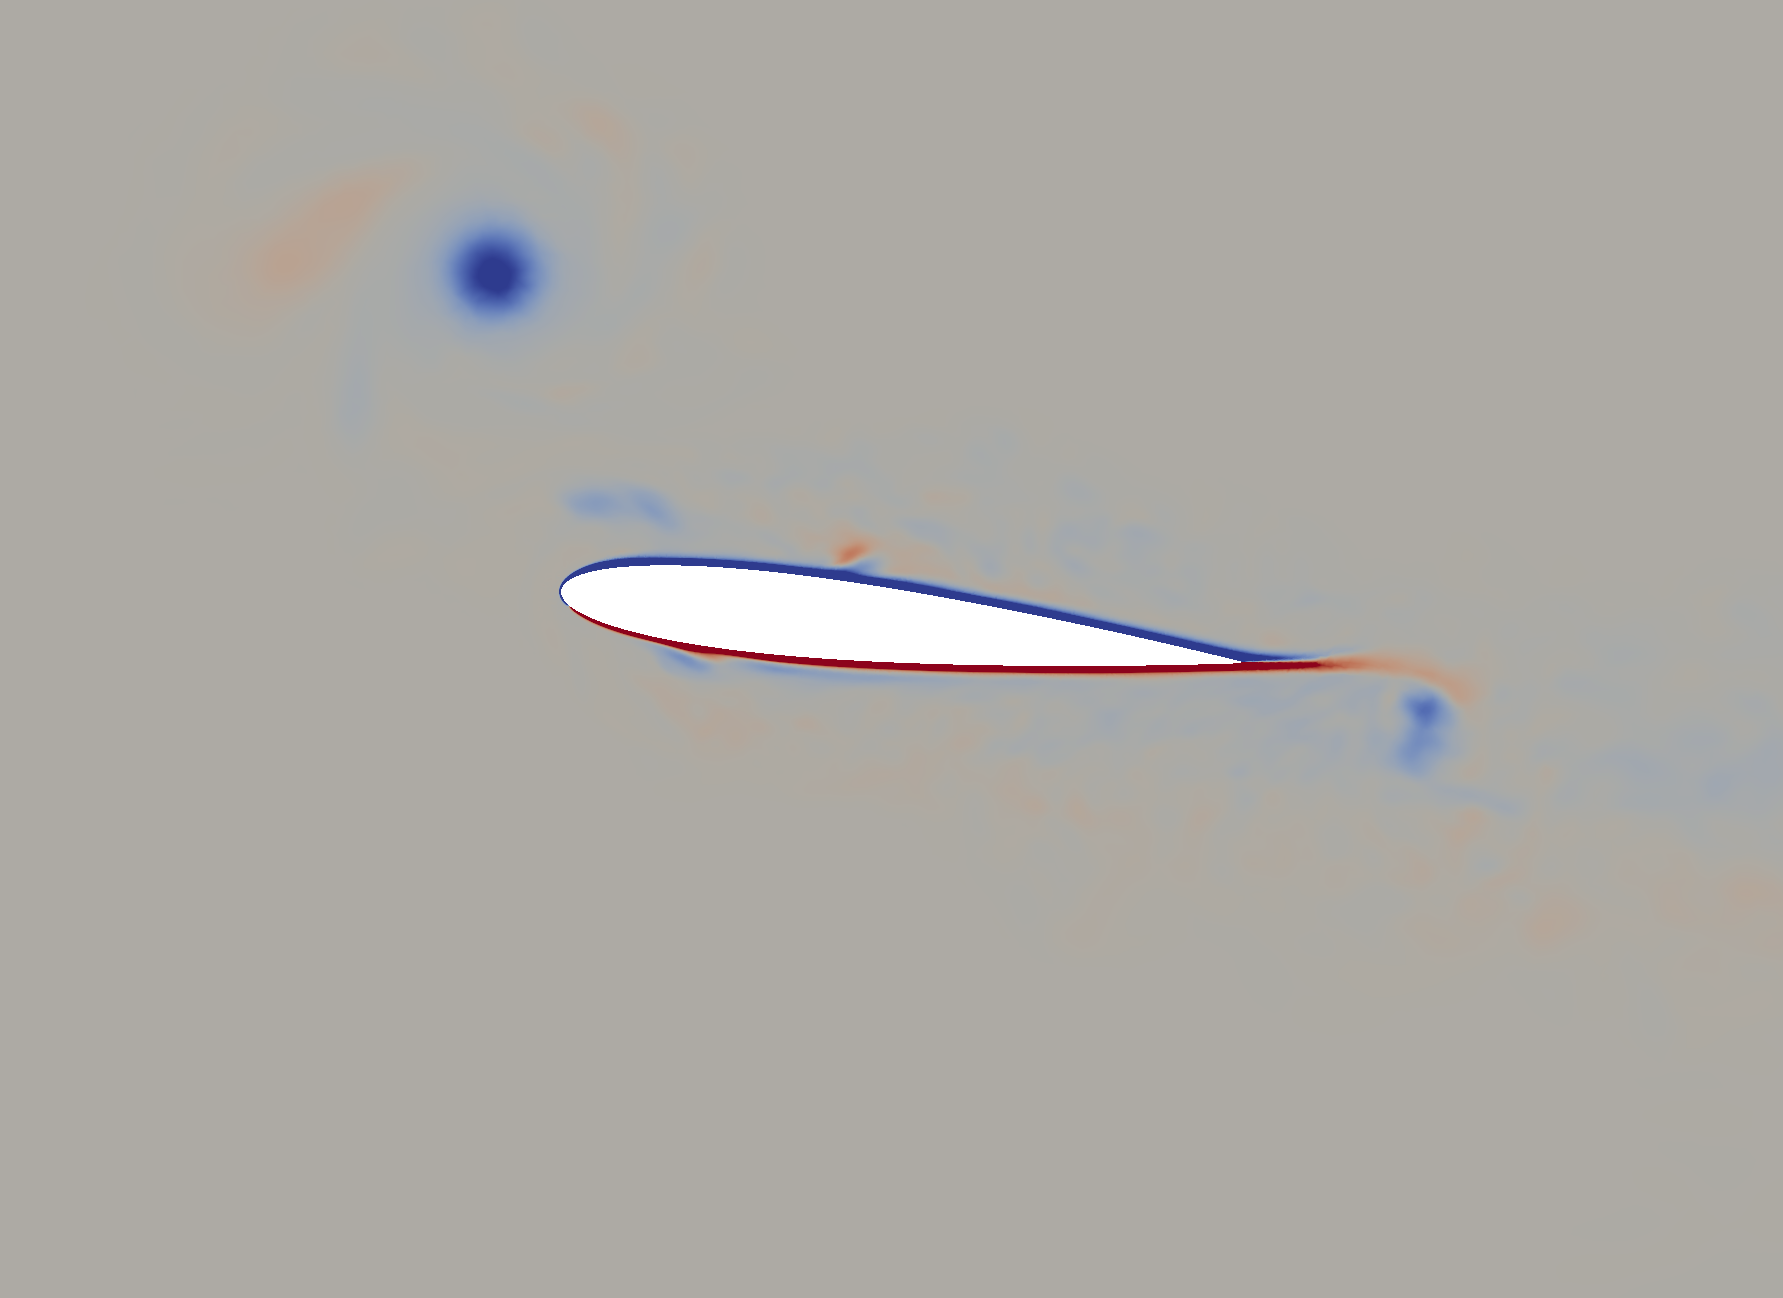
\includegraphics[width=1\textwidth]{figures/Vorticity_plots/Re_40k_1pt2/phase_330.png}
		\caption{$Re=4e4$, $\psi$ = $330^\circ$, $\tilde{t}=0.917$}
		\label{fig:Re_40k_1pt2_phi330}
	\end{subfigure}
	\begin{subfigure}[b]{0.32\textwidth}
		\centering
		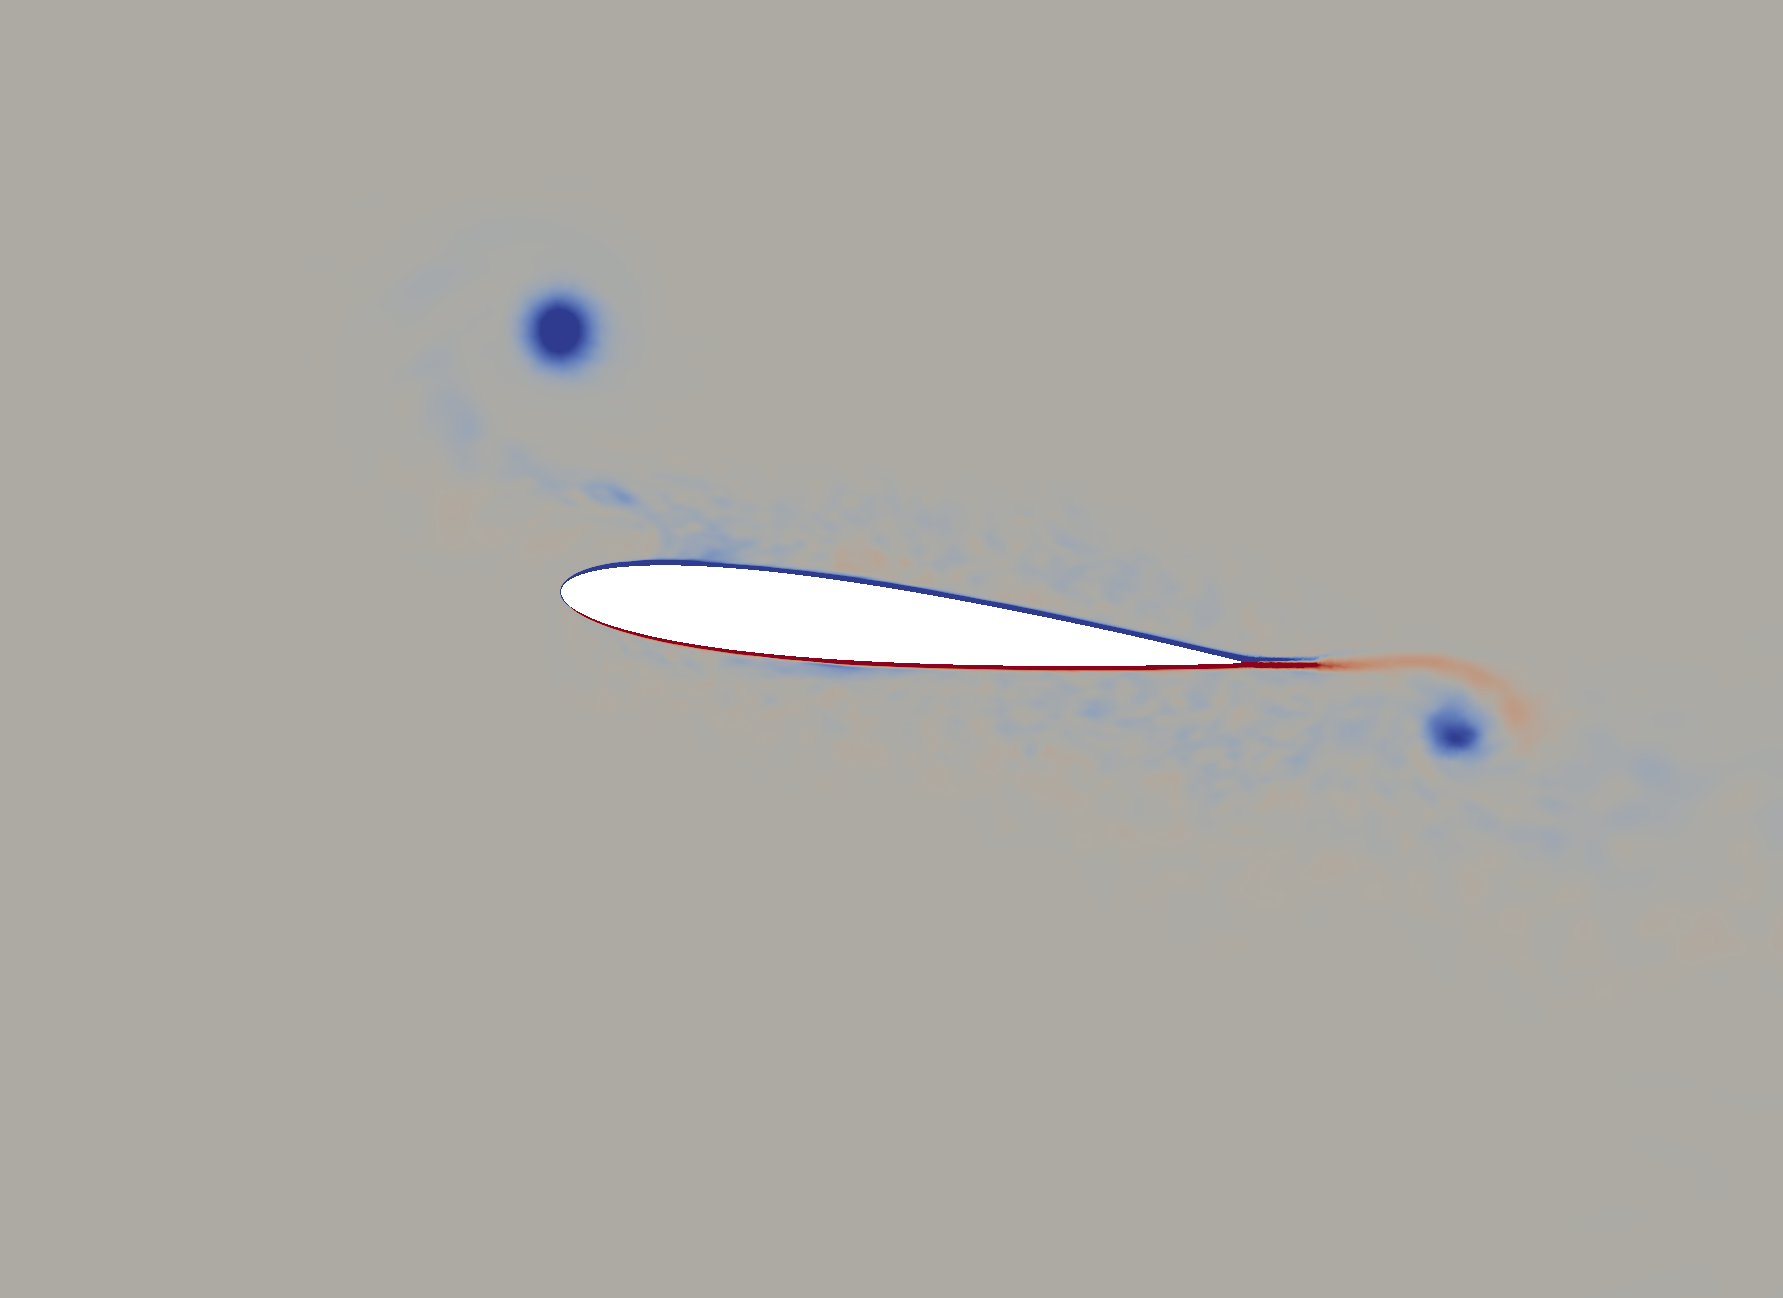
\includegraphics[width=1\textwidth]{figures/Vorticity_plots/Re_200k_1pt2/phase_330.png}
		\caption{$Re=2e5$, $\psi$ = $330^\circ$, $\tilde{t}=0.917$}
		\label{fig:Re_200k_1pt2_phi330}
	\end{subfigure}
	\begin{subfigure}[b]{0.32\textwidth}
		\centering
		\includegraphics[width=1\textwidth]{figures/Vorticity_plots/Re_1m_1pt2/phase_330.png}
		\caption{$Re=1e6$,$\psi$ = $330^\circ$, $\tilde{t}=0.917$}
		\label{fig:Re_1m_1pt2_phi330}
	\end{subfigure}	
	\begin{subfigure}[b]{0.32\textwidth}
		\centering
		\includegraphics[width=1\textwidth]{figures/Vorticity_plots/Re_40k_1pt2/phase_345.png}
		\caption{$Re=4e4$, $\psi$ = $345^\circ$, $\tilde{t}=0.958$}
		\label{fig:Re_40k_1pt2_phi345}
	\end{subfigure}
	\begin{subfigure}[b]{0.32\textwidth}
		\centering
		\includegraphics[width=1\textwidth]{figures/Vorticity_plots/Re_200k_1pt2/phase_345.png}
		\caption{$Re=2e5$, $\psi$ = $345^\circ$, $\tilde{t}=0.958$}
		\label{fig:Re_200k_1pt2_phi345}
	\end{subfigure}
	\begin{subfigure}[b]{0.32\textwidth}
		\centering
		\includegraphics[width=1\textwidth]{figures/Vorticity_plots/Re_1m_1pt2/phase_345.png}
		\caption{$Re=1e6$,$\psi$ = $345^\circ$, $\tilde{t}=0.958$}
		\label{fig:Re_1m_1pt2_phi345}
	\end{subfigure}
	
	\caption{Spanwise vorticity at 8 different phases for $Re$=40,000 (left column), 200,000 (middle column) and 1,000,000 (right column) at $\mu_{sect}$ = 1.2}
	\label{fig:vortScreen_1pt2}
\end{figure}

\subsection{LEV Evolution}
\label{sec:LEV}

%TODO: Use pics from presentation

LEV detection and tracking is performed using the procedure developed in this work, see Section \ref{sec:LEV_detect_track}. LEV position with respect to the leading edge of the airfoil is presented in Figure~\ref{fig:LEV_location_LE_airfoil}.
In the $\mu_{sect}=1.0$ case, the initial position of the LEV (i.e., position at formation) gets closer to the leading edge as the Reynolds number is increased.
Further, LEV remains closest to the airfoil over the cycle for the highest Reynolds number of $Re$=1,000,000 (i.e., note the vertical position of the LEV).
On the other hand, LEV initially moves to the left (towards the geometric leading edge) from its initial position for the lowest Reynolds number of $Re$=40,000.
In the $\mu_{sect}=1.2$ case also, similar trends are observed.
However, at the higher advance ratio the LEV initially moves to the left past the geometric leading edge for each Reynolds number.
This is expected since the relative flow velocity becomes negative (or a reversed flow condition is obtained) at $\mu_{sect}=1.2$.

Figure \ref{fig:LEV_size} presents the size or core radius ($r_c$) of the LEV for all six cases.
We note that in simulations the data was recorded at every $\Delta \psi = 15^\circ$ starting at $\psi$=$15^\circ$.
For each case the LEV is formed at about $\tilde{t}=0.6$ or later.
The LEV size is higher for the lowest Reynolds number of $Re$=40,000 for both advance ratios of $\mu_{sect}$=1.0 and 1.2.
This is expected since the boundary layer is thicker for $Re$=40,000 and the resulting separated shear layer rolls up into a larger LEV.
The LEV size is very similar for the other two higher Reynolds numbers at $\mu_{sect}$=1.0 and 1.2.
In the $\mu_{sect}$=1.0 case, the LEV increases in size till about $\tilde{t}=0.75$ to 0.8 and subsequently seem to plateau or increase in size relatively slowly.
Towards the end of the cycle, the LEV size is predicted to be about 8\% of the chord for $Re$=40,000 at $\mu_{sect}$=1.0, and about 6\% for $Re$=200,000 and 1,000,000 at $\mu_{sect}$=1.0.
In the $\mu_{sect}$=1.2 case, the LEV increases in size throughout the cycle and towards the end of the cycle reaches about a similar size as the $\mu_{sect}$=1.0 case for each Reynolds number. Note that such a quantification of LEV evolution, based on feature/vortex detection and tracking procedure, is also useful for feature-based adaptivity, which is discussed in Section \ref{sec:feature_based_strat}.

\begin{figure}[H]
	\begin{subfigure}{0.5\textwidth}
		\includegraphics[width=1\textwidth]{figures/LEV_size_lambda_1pt0.png}
		\caption{$\mu_{sect} = 1.0$}
		\label{fig:LEV_size_lambda_1p0}
	\end{subfigure}
 	\begin{subfigure}{0.5\textwidth}
	\includegraphics[width=1\textwidth]{figures/LEV_size_lambda_1pt2.png}
	\caption{$\mu_{sect} = 1.2$}
	\label{fig:LEV_size_lambda_1p2}
	\end{subfigure}
 	\caption{LEV evolution: LEV size for $Re$=40,000 (green line with open triangles), 200,000 (red line with closed circles) and 1,000,000 (blue line with open circles) at $\mu_{sect}$=1.0 and 1.2}
 	\label{fig:LEV_size}
\end{figure}




%TODO: indicate we consider Re=40k and 200k for adaptive LES and carefully investigate mesh convergence. this was done for cost savings since LEV exhibits a similar behavior for Re=200k and Re=1m cases.

\begin{figure}[H]
	\begin{subfigure}{0.5\textwidth}
		\includegraphics[width=1\textwidth]{figures/LEV_location_lambda_1pt0}
		\caption{$\mu_{sect} = 1.0$}
		\label{fig:LEV_location_lambda_1p0}
	\end{subfigure}
	\begin{subfigure}{0.5\textwidth}
		\includegraphics[width=1\textwidth]{figures/LEV_location_lambda_1pt2}
		\caption{$\mu_{sect} = 1.2$}
		\label{fig:LEV_location_lambda_1p2}
	\end{subfigure}
 	\caption{LEV evolution: LEV position (with respect to the leading edge of the airfoil) for $Re$=40,000 (green line with open triangles), 200,000 (red line with closed circles) and 1,000,000 (blue line with open circles) at $\mu_{sect}$=1.0 and 1.2}
	\label{fig:LEV_location_LE_airfoil}
\end{figure}

In Figure \ref{fig:LEV_delta_x}, the horizontal displacement of the LEV with respect to the ground is presented.
The displacement is taken about the initial position when the LEV is formed, i.e., the displacement is zero at the initial position.
Again, as the Reynolds number increases the LEV is formed later in the cycle (for a given advance ratio) while as the advance ratio increases it is formed earlier in the cycle (for a given Reynolds number).

An important aspect to note in Figure \ref{fig:LEV_delta_x} is that the horizontal displacement of the LEV follows a straight line for each case and is parallel among all cases.
The slope of the horizontal displacement in each case is remarkably close to the free-stream velocity, i.e., the LEV is advected in the horizontal direction at the free-stream velocity.

\begin{figure}[H]
	\begin{subfigure}{0.5\textwidth}
		\includegraphics[width=1\textwidth]{figures/LEV_deltax_lambda_1pt0.png}
		\caption{$\mu_{sect} = 1.0$}
		\label{fig:LEV_deltax_lambda_1p0}
	\end{subfigure}
	\begin{subfigure}{0.5\textwidth}
		\includegraphics[width=1\textwidth]{figures/LEV_deltax_lambda_1pt2.png}
		\caption{$\mu_{sect} = 1.2$}
		\label{fig:LEV_deltax_lambda_1p2}
	\end{subfigure}
	\caption{LEV evolution: LEV displacement (in the horizontal direction) for $Re$=40,000 (green line with open triangles), 200,000 (red line with closed circles) and 1,000,000 (blue line with open circles) at $\mu_{sect}$=1.0 and 1.2}
	\label{fig:LEV_delta_x}
\end{figure}

\label{sec:baseline_results}

\section{Overview of Adaptive Strategies}

In this section, we focus on the low Reynolds number case of $Re=40,000$ at an angle of attack of $\alpha=6^\circ$ and advance ratio of $\mu_{sect}=1.2$. We explore three different adaptation strategies for mesh adaptation based on the VMS-based estimated error. 

The first strategy we employ is error estimator based zonal refinement/adaptation. 
In this strategy, we obtain an initial solution on a baseline mesh for the problem at hand. The VMS-based error estimator is then applied to the solution corresponding to this mesh, and based on the estimated error, the mesh is refined by a factor of 2 in particular zones where high error values are found. Estimated error for this adapted mesh is then calculated, and the mesh is again refined by a factor of 2 in zones of high error. This process is repeated till it is computationally feasible, or a convergence is reached.

The second strategy we employ is fully automated mesh adaptation based on the VMS-based error estimator. In this strategy, the estimated error and a specified target error are used to compute the desired mesh size or resolution in a local fashion, i.e., at every mesh vertex. We refer to this as the nodal size field, and the mesh is refined or coarsened based on this nodal size field. 

The third strategy is to employ feature-based refinement/adaptation. This allows for refinement around dominant flow features and also along the path/trajectory of such features, for example, the paths of leading and trailing edge vortices (LEV and TEV) over a surging cycle using vortex tracking. By running an initial simulation, we can get information on the approximate path that a certain feature will follow, estimate the error along this path, and perform refinement/adaptation along this path. 

Further details and applications of these three strategies are included in the following sections.

\subsection{Zonal Refinement/Adaptation}
In this strategy, an initial solution is obtained on an initial mesh with a set of canonical refinement zones that are usually used for a flow over an airfoil. We refer to this mesh as M0\_nz25, see Figure \ref{fig:M0_mesh}. In-plane mesh sizes are indicated in the figure. The initial mesh spacing/resolution on the surface of the airfoil in the streamwise and spanwise directions is set to be below 75 and 40 in wall units, respectively.
Here nz25 refers to the number of spanwise extruded layers (i.e., 25) used in this mesh. 
As mentioned before, the VMS-based error estimator is applied to phase-averaged data, and the maximum error value over multiple phases (i.e., at 24 equispaced phases over the surging cycle), and over the spanwise direction, is selected to represent the element-level local error within the airfoil plane/section throughout the surging cycle. 
The element-level error estimated on this mesh is shown in Figure \ref{fig:M0_err_plot}. 
We can see that higher errors are observed primarily in the regions traversed by the LEV through the surging cycle, as well as in the wake of the airfoil. 
Higher errors are also observed close to the airfoil surface and in the boundary layer region.

Based on the estimated error, the mesh is refined by a factor of 2 in zones where high error values are found, including in the boundary layer mesh (i.e., along the streamwise direction). 
The spanwise resolution is also refined by a factor of 2 (i.e., the number of layers in the spanwise direction is doubled). 
This adapted mesh is shown in Figure \ref{fig:Mza1_mesh} and the estimated error on it is shown in Figure \ref{fig:Mza1_err_plot}. It is referred to as the Mza1\_nz50 mesh (where za is short for zonal adaptation and 1 in za1 denotes the first iteration of mesh adaptation).
%It is observed that the error has approximately reduced by a factor of 4 in the Mza1\_nz50 mesh as compared to the M0 mesh.
It is observed that the error has reduced in the Mza1\_nz50 mesh as compared to the M0 mesh
These meshes, M0\_nz25 and Mza1\_nz50, consist of 774,525 and 2,874,300 elements, respectively.

%Zonal refinements are added to the Mza1 mesh in regions of high error, and the mesh is refined further by a factor of 2 in these zones, along with the boundary layer mesh in the streamwise direction, and the number of layers in the spanwise direction is doubled.  This mesh, which is referred to as Mza2, is shown in Figure \ref{fig:Mza2_mesh}. Again, we observe that the error has reduced by a factor of 4 in the Mz\_a2 mesh as compared to Mz\_a1 mesh.

%The number of elements for each mesh is presented in Table \ref{table:mesh_zonal_summary}.


% \begin{table}[H]
% 	\centering
% 	\caption{Summary of zonal refinement based meshes}
% 	\label{table:mesh_zonal_summary}
% 	\begin{tabular}{|l|c|c|c|c|c|}
% 		\hline
% 		Mesh case  & No. of elements\\
% 		\hline
% 		\hline
% 		M0\_nz25 & 774,525 \\
% 		\hline
% 		Mza1\_nz50 &  2,874,300 \\
% 		\hline
% %		Mz\_a2 & 14,329,200 \\
% %		\hline
% 	\end{tabular}
	
% \end{table}

A comparison of different adaptive strategies/adapted meshes is provided in Section \ref{sec:results_adapt}.

\begin{figure}[H]
\centering
\begin{subfigure}[b]{0.475\textwidth}
\centering
\includegraphics[width=1\textwidth]{figures/adapt_strat/M0_mesh.png}
\caption{M0\_nz25 mesh}
\label{fig:M0_mesh}
\end{subfigure}
\begin{subfigure}[b]{0.475\textwidth}
\centering
\includegraphics[width=1\textwidth]{figures/adapt_strat/M0_error.png}
\caption{M0\_nz25 error field}
\label{fig:M0_err_plot}
\end{subfigure}
\begin{subfigure}[b]{0.475\textwidth}
\centering
\includegraphics[width=1\textwidth]{figures/adapt_strat/Mza1_mesh.png}
\caption{Mza1\_nz50 mesh}
\label{fig:Mza1_mesh}
\end{subfigure}
\begin{subfigure}[b]{0.475\textwidth}
\centering
\includegraphics[width=1\textwidth]{figures/adapt_strat/Mza1_error.png}
\caption{Mza1\_nz50 error field}
\label{fig:Mza1_err_plot}
\end{subfigure}
%\begin{subfigure}[b]{0.475\textwidth}
%\centering
%\includegraphics[width=1\textwidth]{figures/adapt_strat/Mza2_mesh.png}
%\caption{Mz\_a2 mesh}
%\label{fig:Mza2_mesh}
%\end{subfigure}
%\begin{subfigure}[b]{0.475\textwidth}
%\centering
%\includegraphics[width=1\textwidth]{figures/adapt_strat/Mza2_error_plot.png}
%\caption{Mz\_a2 error field}
%\label{fig:Mza2_err_plot}
%\end{subfigure}
\caption{Meshes and estimated error fields for zonal-based strategy}
\end{figure}



\subsection{Nodal Size Field-based Adaptation}
In this adaptive strategy, the VMS-based error is calculated on the initial mesh. Based on the estimated error, a nodal size field is calculated using the following equation \cite{zhang19}

\begin{equation}
\frac{e_k}{\tilde{e}_k} = \left(\frac{h_{old}}{h_{new}}\right)^{m+N/2} 
\label{eq:diez}
\end{equation}

Here, $e_k$ is the measured local error (in the $\HOne$-seminorm) at an element $k$, $\tilde{e}_k$ is the target error for an element specified by the user, $m$ is the polynomial order of the approximation space (i.e., $m=1$ for the linear finite elements used currently) , and $N$ is the number of spatial dimensions. $h_{old}$ is current size of the element, and $h_{new}$ is the desired new mesh size.
This new mesh size at the element level is assembled at the node/vertex level to perform mesh adaptation.

\begin{figure}[H]
\centering

\begin{subfigure}[b]{0.475\textwidth}
\centering
\includegraphics[width=1\textwidth]{figures/adapt_strat/h_adapt1_mesh.png}
\caption{Ms\_a1 mesh}
\label{fig:h_adapt1_mesh}
\end{subfigure}
\begin{subfigure}[b]{0.475\textwidth}
\centering
\includegraphics[width=1\textwidth]{figures/adapt_strat/h_adapt1_error_plot.png}
\caption{Ms\_a1 error field}
\label{fig:h_adapt1_error_plot}
\end{subfigure}

\caption{Mesh and estimated error for size-based refinement strategy (Ms\_a1)}
\end{figure}

For the surging airfoil case, M0 is used as the initial mesh (Figure \ref{fig:M0_mesh}) and the corresponding error estimated on M0 mesh (Figure \ref{fig:M0_err_plot}) is used to calculate $h_{new}$. The mesh refinement is controlled to have a maximum refinement and maximum coarsening of a factor of 2 to avoid excessive refinement or coarsening in a local region. The mesh obtained using this strategy is shown in Figure \ref{fig:h_adapt1_mesh}. Note that in terms of mesh resolution, this mesh compares best against Mz\_a1 from zonal refinement strategy. This mesh consists of 2,859,450 elements, which is comparable to 2,874,300 elements for the Mz\_a1 mesh. The major differences between the two meshes is that Mz\_a1 maintains the same mesh size in various zones, whereas the Ms\_a1 mesh is patchy, i.e., a uniform refinement is not maintained within regions of interest.
The corresponding estimated error for this mesh is shown in Figure \ref{fig:h_adapt1_error_plot}. Comparing the estimated error to Mz\_a1 mesh, higher error values are observed for Ms\_a1 in the LEV region, as well as in the wake of the airfoil. A more thorough comparison of results is mentioned in Section \ref{sec:results_adapt}.


\subsection{Feature-based Refinement/Adaptation}
In this strategy, mesh refinement is applied around the dominant flow features of interest.
In the current surging airfoil case, LEV is the dominant flow feature. 
Using vortex detection and tracking (see Section \ref{sec:LEV_detect_track}), LEV evolution (path and size) is determined using an initial mesh (M0\_nz25 in this case). 
Based on this a refinement zone is added around the path of the LEV.
In such a feature-based refinement, VMS-based estimated error is used to set the mesh size in the refinement zone(s) around the dominant feature(s). 
In addition, estimated error is also used to refine the mesh around the airfoil (e.g., in a similar fashion as the error-based zonal refinement discussed earlier). 
This is done to accurately resolve the flow near the airfoil including the boundary layer region that plays a direct role in the formation of LEV.

In summary, the mesh around the LEV path is refined by a factor of 2. In addition, the boundary layer mesh is refined by a factor of 2 in the streamwise direction, and again, the number of layers in the spanwise direction are doubled as compared to M0\_nz25.
The resulting mesh resolution on the surface of the airfoil in the streamwise and spanwise directions is below 40 and 25 in wall units, respectively, i.e., same as the previous cases.
This adapted mesh is referred to as the Mfa1\_nz50 mesh (where fa is short for feature-based adaptation and 1 in fa1 denotes the first iteration of mesh adaptation). 
This mesh is shown in Figure \ref{fig:FB_mesh} and the estimated error on it is shown in Figure \ref{fig:FB_error_plot}.
M0\_nz0 mesh and error field are shown again to compare against Mfa1\_nz50.
Mfa1\_nz50 contains 2,777,750 elements, which is comparable to both Mza1\_nz50 and Msa1\_nz50 meshes.

Error values are similar to those obtained on the Mza1\_nz50 mesh, i.e., near the airfoil surface, in the LEV path, and in the wake, since mesh resolution in crucial regions is similar between the Mfa1\_nz50 and Mza1\_nz50 meshes, while estimated error is higher on the Msa1\_nz50 mesh.
%Error values are lower as compared to Msa1\_nz50, since a uniform mesh size is maintained, as opposed to Msa1\_nz50, where the mesh size is patchy.
A more detailed comparison of different adaptive strategies/adapted meshes is provided in Section \ref{sec:results_adapt}.

\begin{figure}[H]
\centering
\begin{subfigure}[b]{0.475\textwidth}
\centering
\includegraphics[width=1\textwidth]{figures/adapt_strat/M0_mesh.png}
\caption{M0\_nz25 mesh}
\label{fig:M0_mesh_fa}
\end{subfigure}
\begin{subfigure}[b]{0.475\textwidth}
\centering
\includegraphics[width=1\textwidth]{figures/adapt_strat/M0_error.png}
\caption{M0\_nz25 error field}
\label{fig:M0_err_plot_fa}
\end{subfigure}
\begin{subfigure}[b]{0.475\textwidth}
\centering
\includegraphics[width=1\textwidth]{figures/adapt_strat/Mfa1_mesh.png}
\caption{Mfa1\_nz50 mesh}
\label{fig:FB_mesh}
\end{subfigure}
\begin{subfigure}[b]{0.475\textwidth}
\centering
\includegraphics[width=1\textwidth]{figures/adapt_strat/Mfa1_error.png}
\caption{Mfa1\_nz50 error field}
\label{fig:FB_error_plot}
\end{subfigure}

\caption{Meshes and estimated error fields for feature-based strategy}
\end{figure}
\label{sec:feature_based_strat}


\subsection{Results using Different Adaptive Strategies}
In this section, we compare results for the surging airfoil case based on meshes obtained from different adaptive strategies mentioned above. 
We compare different quantities of interest. 
A comparison of force response in the form of normalized lift and drag forces is shown in Figures \ref{fig:lift_plot} and \ref{fig:drag_plot} respectively. The normalized lift matches up well for all the meshes considered. Normalized drag shows differences only for Mz\_a2 mesh (the finest mesh), specifically between phases $\psi=160^\circ$ and $\psi=240^\circ$ whereas the drag response for all the other meshes matches up well.

A comparison of spanwise vorticity for the different meshes is shown in Figures\ref{fig:vorticity_195}, \ref{fig:vorticity_210}, and \ref{fig:vorticity_270} for phases $\psi=210^\circ$, $\psi=225^\circ$, and $\psi=270^\circ$, respectively.
For $\psi=195^\circ$, as the airfoil is in the retreating phase, boundary layer roll-up towards the geometric leading edge is observed over the airfoil surface. For the meshes based on zonal refinement, as we go from M0 to Mz\_a1 and Mz\_a2, the separation over the airfoil is well resolved, and more structures are visible as the mesh becomes finer. Comparing Mz\_a1, Ms\_a1, and Mf\_a1 meshes, we can see that Ms\_a1 mesh does not capture the fine-scale flow structures as compared to the Mz\_a1 mesh, both over the airfoil surface and in the wake of the airfoil. On the other hand, the Mf\_a1 mesh captures these fine-scale flow structures.

\begin{figure}[H]
\centering

\begin{subfigure}[b]{0.7\textwidth}
\centering
\includegraphics[width=1\textwidth]{figures/Results/Lift_plot.png}
\caption{Normalized lift}
\label{fig:lift_plot}
\end{subfigure}
\begin{subfigure}[b]{0.7\textwidth}
\centering
\includegraphics[width=1\textwidth]{figures/Results/Drag_plot.png}
\caption{Normalized drag}
\label{fig:drag_plot}
\end{subfigure}

\label{fig:force_response_adapt}
\caption{Normalized forces for different meshes}
\end{figure}

%Next, we look at the location of the LEV core for different meshes in Figure \ref{fig:LEV_location}. Some differences in the LEV location for various phases are observed. LEV location for Ma1, FB, and hadapt meshes is similar in the beginning phases. Ma1 starts to deviate from FB and hadapt in the later phases. LEV location for FB and hadapt meshes start to match with Ma2 in the later phases, whereas M0 LEV location fluctuates around the other meshes. This however is still not conclusive as to which mesh performs better and a more quantitative study is needed.


%%\begin{figure}[H]
%\centering
%\includegraphics[width=0.7\textwidth]{figures/Results/LEV_location.png}
%\caption{LEV location for different meshes}
%\label{fig:LEV_location}
%\end{figure}
%%


For $\psi=210^\circ$, formation of LEV begins to take place, as we see a distinct vortex build up near the geometric leading edge. At this phase, the differences in the structures resolved by the different meshes become more clear, with Mz\_a2 being the most resolved. Similar to $\psi=195$, the Ms\_a1 mesh shows poor resolution of the fine-scale flow structures as compared to  Mz\_a1 and Mf\_a1 meshes.

For $\psi=270^\circ$, differences can be seen in the shear layer at the geometric leading edge of the airfoil, and the resolution of the LEV. The LEV and the shear layer are best resolved for Mz\_a2 and Mf\_a1 meshes. Recall that Mf\_a1 is obtained using feature-based mesh refinement designed to resolve the LEV accurately, and has the same mesh resolution as Mz\_a2 along the path of the LEV. Once again, shear layer is not well resolved for Ms\_a1 as compared to other refined/adapted meshes.

The poor resolution of the flow-field observed for Ms\_a1 can be attributed to the mesh not having a uniform refinement in the regions of interest, having been adapted solely based on the error-field obtained, which results in a patchy mesh, i.e., the mesh size does not remain constant in particular zones, and hence, structures are not resolved as desired.

\begin{figure}[H]
\centering
\begin{subfigure}[b]{0.475\textwidth}
\centering
\includegraphics[width=1.25\textwidth]{figures/vorticity_plots/M0/ph_195.png}
\caption{M0 mesh, $\psi$ = $195^\circ$}
\label{fig:M0_psi195}
\end{subfigure}
\begin{subfigure}[b]{0.475\textwidth}
\centering
\includegraphics[width=1.25\textwidth]{figures/vorticity_plots/Mza1/ph_195.png}
\caption{Mz\_a1 mesh, $\psi$ = $195^\circ$}
\label{fig:Ma1_psi195}
\end{subfigure}
\begin{subfigure}[b]{0.475\textwidth}
\centering
\includegraphics[width=1.25\textwidth]{figures/vorticity_plots/Mza2/ph_195.png}
\caption{Mz\_a2 mesh, $\psi$ = $195^\circ$}
\label{fig:Ma2_psi195}
\end{subfigure}
\begin{subfigure}[b]{0.475\textwidth}
\centering
\includegraphics[width=1.25\textwidth]{figures/vorticity_plots/SB/ph_195.png}
\caption{Ms\_a1 mesh, $\psi$ = $195^\circ$}
\label{fig:hadapt_psi195}
\end{subfigure}

\begin{subfigure}[b]{0.475\textwidth}
\centering
\includegraphics[width=1.25\textwidth]{figures/vorticity_plots/FB/ph_195.png}
\caption{Mf\_a1 mesh, $\psi$ = $195^\circ$}
\label{fig:FB_psi195}
\end{subfigure}
\caption{Spanwise vorticity comparison at $\psi$ = $195^\circ$ for different meshes}
\label{fig:vorticity_195}
\end{figure}



\begin{figure}[H]
\centering
\begin{subfigure}[b]{0.475\textwidth}
\centering
\includegraphics[width=1.25\textwidth]{figures/vorticity_plots/M0/ph_210.png}
\caption{M0 mesh, $\psi$ = $210^\circ$}
\label{fig:M0_psi210}
\end{subfigure}
\begin{subfigure}[b]{0.475\textwidth}
\centering
\includegraphics[width=1.25\textwidth]{figures/vorticity_plots/Mza1/ph_210.png}
\caption{Mz\_a1 mesh, $\psi$ = $210^\circ$}
\label{fig:Ma1_psi210}
\end{subfigure}
\begin{subfigure}[b]{0.475\textwidth}
\centering
\includegraphics[width=1.25\textwidth]{figures/vorticity_plots/Mza2/ph_210.png}
\caption{Mz\_a2 mesh, $\psi$ = $210^\circ$}
\label{fig:Ma2_psi210}
\end{subfigure}
\begin{subfigure}[b]{0.475\textwidth}
\centering
\includegraphics[width=1.25\textwidth]{figures/vorticity_plots/SB/ph_210.png}
\caption{Ms\_a1 mesh, $\psi$ = $210^\circ$}
\label{fig:hadapt_psi210}
\end{subfigure}
\begin{subfigure}[b]{0.475\textwidth}
\centering
\includegraphics[width=1.25\textwidth]{figures/vorticity_plots/FB/ph_210.png}
\caption{Mf\_a1 mesh, $\psi$ = $210^\circ$}
\label{fig:FB_psi210}
\end{subfigure}
\caption{Spanwise vorticity comparison at $\psi$ = $210^\circ$ for different meshes}
\label{fig:vorticity_210}
\end{figure}



%%VORTICITY PLOT
\begin{figure}[H]
\centering

\begin{subfigure}[b]{0.475\textwidth}
\centering
\includegraphics[width=1.25\textwidth]{figures/vorticity_plots/M0/ph_270.png}
\caption{M0 mesh, $\psi$ = $270^\circ$}
\label{fig:M0_psi270}
\end{subfigure}
\begin{subfigure}[b]{0.475\textwidth}
\centering
\includegraphics[width=1.25\textwidth]{figures/vorticity_plots/Mza1/ph_270.png}
\caption{Mz\_a1 mesh, $\psi$ = $270^\circ$}
\label{fig:Ma1_psi270}
\end{subfigure}
\begin{subfigure}[b]{0.475\textwidth}
\centering
\includegraphics[width=1.25\textwidth]{figures/vorticity_plots/Mza2/ph_270.png}
\caption{Mz\_a2 mesh, $\psi$ = $270^\circ$}
\label{fig:Ma2_psi270}
\end{subfigure}
\begin{subfigure}[b]{0.475\textwidth}
\centering
\includegraphics[width=1.25\textwidth]{figures/vorticity_plots/SB/ph_270.png}
\caption{Ms\_a1 mesh, $\psi$ = $270^\circ$}
\label{fig:hadapt_psi270}
\end{subfigure}
\begin{subfigure}[b]{0.475\textwidth}
\centering
\includegraphics[width=1.25\textwidth]{figures/vorticity_plots/FB/ph_270.png}
\caption{Mf\_a1 mesh, $\psi$ = $270^\circ$}
\label{fig:FB_psi270}
\end{subfigure}
\caption{Spanwise vorticity comparison at $\psi$ = $270^\circ$ for different meshes}
\label{fig:vorticity_270}
\end{figure}

For a more quantitative comparison, we focus on $C_p$  at different phases of interest leading up to LEV formation. $C_p$ is shown in Figure \ref{fig:Cp_plots} at six phases for all meshes. At $\psi=180^\circ$, we can see that flow has started to separate for Mz\_a2 mesh around $x/c=0.1$, whereas for all the other meshes, the flow remains attached. For $\psi=195^\circ$, Mz\_a2 and Ms\_a1 meshes show clear signs of separation and LEV formation/boundary layer roll-up, whereas the other meshes do not. Although note that the location and $C_p$ curve for Mz\_a2 and Ms\_a2 meshes are quite different, and separation is detected further downstream for Mz\_a2. For $\psi=210^\circ$, LEV formation is seen for all meshes 
apart from M0 mesh. $\psi=225^\circ$ shows LEV formation and flow separation for all meshes, with clear differences in separation location and $C_p$ curve for all the meshes. Note that the y-axis limits vary for different phases to highlight differences in $C_p$,.
$\psi=270^\circ$ and $\psi=285^\circ$ also show differences in $C_p$ at the geometric trailing edge when the trailing edge vortex starts forming. 

%%Cp plots

\begin{figure}[H]
\centering

\begin{subfigure}[b]{0.475\textwidth}
\centering
\includegraphics[width=1\textwidth]{figures/Results/Cp_plots/Cp_ph_180.png}
\caption{ $C_p$ at $\psi$ = $180^\circ$}
\label{fig:Cp_180}
\end{subfigure}
\begin{subfigure}[b]{0.475\textwidth}
\centering
\includegraphics[width=1\textwidth]{figures/Results/Cp_plots/Cp_ph_195.png}
\caption{ $C_p$ at $\psi$ = $195^\circ$}
\label{fig:Cp_195}
\end{subfigure}
\begin{subfigure}[b]{0.475\textwidth}
\centering
\includegraphics[width=1\textwidth]{figures/Results/Cp_plots/Cp_ph_210.png}
\caption{ $C_p$ at $\psi$ = $210^\circ$}
\label{fig:Cp_210}
\end{subfigure}
\begin{subfigure}[b]{0.475\textwidth}
\centering
\includegraphics[width=1\textwidth]{figures/Results/Cp_plots/Cp_ph_225.png}
\caption{ $C_p$ at $\psi$ = $225^\circ$}
\label{fig:Cp_225}
\end{subfigure}
\begin{subfigure}[b]{0.475\textwidth}
\centering
\includegraphics[width=1\textwidth]{figures/Results/Cp_plots/Cp_ph_270.png}
\caption{ $C_p$ at $\psi$ = $270^\circ$}
\label{fig:Cp_270}
\end{subfigure}
\begin{subfigure}[b]{0.475\textwidth}
\centering
\includegraphics[width=1\textwidth]{figures/Results/Cp_plots/Cp_ph_285.png}
\caption{ $C_p$ at $\psi$ = $285^\circ$}
\label{fig:Cp_285}
\end{subfigure}
\caption{$C_p$ comparison for different meshes. Top surface $C_p$ is denoted by solid lines and bottom surface $C_p$ is denoted by dashed lines}
\label{fig:Cp_plots}
\end{figure}


In summary, mesh refinement/adaptation is necessary to perform accurate LES of complex aerodynamic problems.
\label{sec:results_adapt}




\section{Application of Zonal Refinement Strategy}


In chapter \ref{sec:adaptive_strategy_comparison}, we established that the zonal based refinement/adaptation is the best strategy for accurate numerical solution of periodic problems in space and time using VMS-based error estimator driven mesh adaptation. In this chapter, we focus on applying the zonal based adaptation/refinement strategy. the zonal based refinement strategy is applied to two Reynolds numbers of $Re=40,000$ and $Re=200,000$, at angle of attack $\alpha=6^\circ$ and advance ratio of $\mu_{sect}=1.2$

We explore mesh resolution effects in the in-plane and also in the spanwise direction. 
The run plan to achieve mesh convergence is as follows. 
We start off with an initial mesh that satisfies LES surface resolution criteria for wall-bounded flows. This mesh is referred to as M0.
We obtain the maximum error over all phases through the surging cycle and also maximum in the spanwise direction.
The in-plane mesh is then refined by a factor of 2 in regions of high error zones, i.e., we employ the zonal-based adaptation/refinement strategy.
This resultant mesh is the in-plane mesh after the first adaptation cycle, which is referred to as Mza1.
Here, multiple spanwise resolutions are considered, starting with the spanwise resolution of M0 mesh, to obtain a series of meshes for Mza1 with different spanwise resolutions.
In this series of meshes, spanwise resolution is refined by a factor of 2, till spanwise convergence is achieved for this adaptation cycle. 
For the next adaptation cycle, zonal-based adaptation/refinement is again employed to refine the mesh in the in-plane direction, and the mesh with the second highest spanwise resolution of the previous adaptation cycle is used as the initial spanwise resolution for the current adaptation cycle. 
This mesh is referred to as Mza2.
Multiple spanwise resolutions are considered again for this adaptation cycle.
This process is repeated for further adaptation cycles till mesh convergence is achieved.

\subsection{ $Re=40,000$}

In this section, we focus on applying the zonal based adaptation/refinement strategy to the low Reynolds number case of $Re=40,000$ at angle of attack $\alpha=6^\circ$ and advance ratio of $\mu_{sect}=1.2$ till we obtain mesh convergence.
We start with a baseline mesh that satisfies LES surface resolution criteria in wall plus units at maximum Reynolds number, which is achieved at $\psi=90^\circ$ (since relative velocity over the airfoil is maximum at this phase). 
This mesh is referred to as M0\_nz25, where nz25 refers to the number of extruded layers in the spanwise/z direction.

Next, Mza1 series of meshes is obtained using zonal-based adaptation/refinement, and multiple spanwise resolutions are considered, starting with Mza1\_nz25, and refining by a factor of 2 in spanwise direction to get Mza1\_nz50 and Mza1\_nz100.
We observed that Mza1\_nz25 results compare well both Mza1\_nz50 and Mza1\_nz100 meshes.
Results for Mza1\_nz25 and Mza1\_nz50 meshes are shown in the following sections.
Results for Mza1\_nz100 are omitted for conciseness.

For the next adaptation cycle, Mza2 series of meshes is obtained by applying  zonal-based adaptation/refinement to Mza1\_nz25 mesh.
Initial spanwise resolution of Mza2\_nz25, i.e., 25 spanwise extruded layers is chosen, along with factor of 2 spanwise refinement to get Mza2\_nz50 and Mza2\_nz100 meshes. 
We observed that results from Mza2\_nz25 did not agree well with Mza2\_nz50 mesh, whereas Mza2\_nz50 and Mza2\_nz100 meshes showed good agreement.
Results for Mza2\_nz50 and Mza2\_nz100 meshes are shown in the following sections, while results for Mza2\_nz25 are omitted for conciseness.

For the next adaptation cycle, Mza3 series of meshes is obtained by applying  zonal-based adaptation/refinement to Mza2\_nz50 mesh. 
Initial spanwise resolution of Mza3\_nz50 is chosen, along with factor of 2 spanwise refinement to get Mza3\_nz100. 
We would like to note that Mza3\_nz200 mesh was not computationally feasible, so we stop at Mza3\_nz100.
Results for both Mza3\_nz50 and Mza3\_nz100 are shown in the following sections.

\subsubsection{Adapted Meshes}
\begin{figure}[H]
\centering

\begin{subfigure}[b]{0.475\textwidth}
\centering
\includegraphics[width=1\textwidth]{figures/zonal_adapt_results/Mesh_and_error_plots/M0_inplane.png}
\caption{M0 mesh}
\label{fig:zonal_M0_mesh}
\end{subfigure}
\begin{subfigure}[b]{0.475\textwidth}
\centering
\includegraphics[width=1\textwidth]{figures/zonal_adapt_results/Mesh_and_error_plots/M0_error.png}
\caption{M0\_nz25 error field}
\label{fig:zonal_M0_error}
\end{subfigure}

\begin{subfigure}[b]{0.475\textwidth}
	\centering
	\includegraphics[width=1\textwidth]{figures/zonal_adapt_results/Mesh_and_error_plots/Mza1_inplane.png}
	\caption{Mza1 mesh}
	\label{fig:zonal_Mza1_mesh}
\end{subfigure}
\begin{subfigure}[b]{0.475\textwidth}
	\centering
	\includegraphics[width=1\textwidth]{figures/zonal_adapt_results/Mesh_and_error_plots/Mza1_error.png}
	\caption{Mza1\_nz25 error field}
	\label{fig:zonal_Mza1_error}
\end{subfigure}


\begin{subfigure}[b]{0.475\textwidth}
	\centering
	\includegraphics[width=1\textwidth]{figures/zonal_adapt_results/Mesh_and_error_plots/Mza2_inplane.png}
	\caption{Mza2 mesh}
	\label{fig:zonal_Mza2_mesh}
\end{subfigure}
\begin{subfigure}[b]{0.475\textwidth}
	\centering
	\includegraphics[width=1\textwidth]{figures/zonal_adapt_results/Mesh_and_error_plots/Mza2_error.png}
	\caption{Mza2\_nz50 error field}
	\label{fig:zonal_Mza2_error}
\end{subfigure}

\begin{subfigure}[b]{0.475\textwidth}
	\centering
	\includegraphics[width=1\textwidth]{figures/zonal_adapt_results/Mesh_and_error_plots/Mza3_inplane.png}
	\caption{Mza2 mesh}
	\label{fig:zonal_Mza3_mesh}
\end{subfigure}
\begin{subfigure}[b]{0.475\textwidth}
	\centering
	\includegraphics[width=1\textwidth]{figures/zonal_adapt_results/Mesh_and_error_plots/Mza3_error.png}
	\caption{Mza3\_nz50 error field}
	\label{fig:zonal_Mza3_error}
\end{subfigure}


\caption{Mesh and estimated error}
\end{figure}
\label{sec:zonal_mesh_and_error}

\subsubsection{Force Response}

A comparison of force response in the form of normalized lift and drag forces is shown in Figures \ref{fig:lift_zonal_adapt} and \ref{fig:drag_zonal_adapt} respectively. The normalized lift compares well for all the meshes considered. Normalized drag shows differences for Mza2 meshes and Mza3 meshes from M0 and Mza1 meshes. Maximum drag in the advancing phases is observed around $\psi=270^\circ$, with Mza3 meshes predicting slightly higher drag than Mza2 meshes, followed by Mza1 and M0 meshes. Major differences in drag between different meshes are observed specifically between phases $\psi=160^\circ$ and $\psi=240^\circ$. Between these phases, Mza2 and Mza3 meshes compare well with each other, whereas M0 and Mza1 meshes predict lower drag than Mza2 and Mza3 meshes. Note that lift and drag response remains unaffected with changes in spanwise resolution for the same in-plane mesh.

\begin{figure}[H]
\centering

\begin{subfigure}[b]{0.7\textwidth}
\centering
\includegraphics[width=1\textwidth]{figures/zonal_adapt_results/force_response/Lift.png}
\caption{Normalized lift}
\label{fig:lift_zonal_adapt}
\end{subfigure}
\begin{subfigure}[b]{0.7\textwidth}
\centering
\includegraphics[width=1\textwidth]{figures/zonal_adapt_results/force_response/Drag.png}
\caption{Normalized drag}
\label{fig:drag_zonal_adapt}
\end{subfigure}

\label{fig:force_response_zonal_adapt}
\caption{Normalized forces for different meshes}
\end{figure}
\label{sec:zonal_force_response}

\subsubsection{Flowfield: Spanwise Vorticity}
<<<<<<< HEAD



In this section, we focus on instantaneous spanwise vorticity for the different meshes considered due to zonal-based refinement/adaptation. Here, instantaneous data is considered since we are interested in observing the flow structures and turbulence captured by different meshes, and obtaining phase-averaged data over multiple cycles can be computationally expensive, especially for the finer meshes, and can also filter out the turbulence in the flow-field.

A comparison of instantaneous spanwise vorticity for the different meshes is shown in Figures \ref{fig:vorticity_zonal_150}, \ref{fig:vorticity_zonal_180}, \ref{fig:vorticity_zonal_210}, \ref{fig:vorticity_zonal_240}, and \ref{fig:vorticity_zonal_270} for phases $\psi=150^\circ$, $\psi=180^\circ$, $\psi=210^\circ$, $\psi=240^\circ$, and $\psi=270^\circ$ respectively. 

For $\psi=150^\circ$, as the airfoil decelerates, the boundary layer over the airfoil starts to roll-up towards the geometric leading edge. The finer meshes, Mza2 and Mza3 show a thicker boundary layer along with more resolution of turbulence/fine-scale structures, than
the coarser meshes, M0 and Mza1.

For $\psi=180^\circ$, Mza2 and Mza3 meshes show a thicker boundary layer roll-up towards the geometric leading edge over the airfoil surface, as compared to $\psi=150^\circ$, along with significant flow separation. M0 and Mza1 meshes fail to capture a significant boundary layer roll-up at this phase. Moreover, Mza2 and Mza3 meshes capture more turbulence than M0 and Mza1 meshes, with the flow-structures captured by Mza2 meshes being slightly more diffused than Mza3 meshes. Note that changes in spanwise resolution for the same in-plane mesh do not show any significant variations in the flow-field.

For $\psi=210^\circ$, formation of LEV begins to take place for all meshes apart from M0, as we see a distinct vortex build up near the geometric leading edge, which M0 mesh fails to capture. There is a clear difference between both the location of the roll-up over the airfoil surface, and the size and extent of the roll-up between Mza1 meshes and Mza2 and Mza3 meshes. The flow-field for Mza2 and Mza3 meshes compare well with each other, with some minor differences due to the flow-field being instantaneous. More fine-scale flow structures are resolved by the finer meshes Mza2 and Mza3, while M0 and Mza1 show poor resolution of these structures.

At $\psi=240^\circ$, the LEV has ejected from the airfoil surface into a distinct vortex. Once again, a clear difference can be observed between the coarser meshes (M0 and Mza1 meshes) and the finer meshes Mza2 and Mza3, both in position, size, and extent of the LEV core, and also the turbulence captured around the LEV core. The coarsest mesh, M0, shows poor resolution of the shear layer, LEV, and the fine scale structures around it. Mza1\_25 and Mza1\_50 meshes show a similar location, size, and extent of the LEV, while resolving some diffused flow structures around it. Mza2 and Mza3 meshes compare well with each other in terms of the shear layer, LEV location, size, and extent, as well as the fine scale structures resolved. Once again, note that changes in spanwise resolution for the same in-plane mesh do not show any significant variations in the flow-field. 

At $\psi=270^\circ$, M0 mesh shows poor resolution with a diffused LEV core as compared to the other meshes, along with poor resolution of the shear layer. Mza1 meshes show a less diffused LEV core as compared to M0 mesh, however, the shear layer has comparatively poor resolution when compared to the finer meshes Mza2 and Mza3. Mza1 meshes also show minimal fine scale structures around the LEV core, as compared to Mza2 and Mza3 meshes. The LEV and the shear layer are best resolved in Mza3 meshes, with Mza3 showing more fine scale structures around the LEV core than Mza2 meshes.

A more quantitive comparison of the LEV including tangential velocity profiles and LEV location for different phases in the surging cycle is mentioned in the following sections.

%%=====================================
%% Phase = 150
%%=====================================


\begin{figure}[H]
	\centering
	\begin{center}
		\begin{subfigure}[b]{0.475\textwidth}
			\centering
			\includegraphics[width=1\textwidth]{figures/zonal_adapt_results/vorticity_plots/v2/M0/spavg/phase_150.png}
			\caption{M0 mesh, $\psi$ = $150^\circ$}
			\label{fig:M0_sp_psi150}
		\end{subfigure}
	\end{center}
	\begin{subfigure}[b]{0.475\textwidth}
		\centering
		\includegraphics[width=1\textwidth]{figures/zonal_adapt_results/vorticity_plots/v2/Mza1_25/spavg/phase_150.png}
		\caption{Mza1\_25 mesh, $\psi$ = $150^\circ$}
		\label{fig:Mza1_25_sp_psi150}
	\end{subfigure}
	\begin{subfigure}[b]{0.475\textwidth}
		\centering
		\includegraphics[width=1\textwidth]{figures/zonal_adapt_results/vorticity_plots/v2/Mza1_50/spavg/phase_150.png}
		\caption{Mza1\_50 mesh, $\psi$ = $150^\circ$}
		\label{fig:Mza1_50_sp_psi150}
	\end{subfigure}
	%	\begin{subfigure}[b]{0.475\textwidth}
	%		\centering
	%		\includegraphics[width=1\textwidth]{figures/zonal_adapt_results/vorticity_plots/v2/Mza1_100/spavg/phase_150.png}
	%		\caption{Mza1\_100 mesh, $\psi$ = $150^\circ$}
	%		\label{fig:Mza1_100_sp_psi150}
	%	\end{subfigure}
	%	\begin{subfigure}[b]{0.475\textwidth}
	%	\centering
	%	\includegraphics[width=1\textwidth]{figures/zonal_adapt_results/vorticity_plots/v2/Mza2_25/spavg/phase_150.png}
	%	\caption{Mza2\_25 mesh, $\psi$ = $150^\circ$}
	%	\label{fig:Mza2_25_sp_psi150}
	%	\end{subfigure}
	\begin{subfigure}[b]{0.475\textwidth}
		\centering
		\includegraphics[width=1\textwidth]{figures/zonal_adapt_results/vorticity_plots/v2/Mza2_50/spavg/phase_150.png}
		\caption{Mza2\_50 mesh, $\psi$ = $150^\circ$}
		\label{fig:Mza2_50_sp_psi150}
	\end{subfigure}	
	\begin{subfigure}[b]{0.475\textwidth}
		\centering
		\includegraphics[width=1\textwidth]{figures/zonal_adapt_results/vorticity_plots/v2/Mza2_100/spavg/phase_150.png}
		\caption{Mza2\_100 mesh, $\psi$ = $150^\circ$}
		\label{fig:Mza2_100_sp_psi150}
	\end{subfigure}
	\begin{subfigure}[b]{0.475\textwidth}
		\centering
		\includegraphics[width=1\textwidth]{figures/zonal_adapt_results/vorticity_plots/v2/Mza3_50/spavg/phase_150.png}
		\caption{Mza3\_50 mesh, $\psi$ = $150^\circ$}
		\label{fig:Mza3_100_sp_psi150}
	\end{subfigure}
	\begin{subfigure}[b]{0.475\textwidth}
		\centering
		\includegraphics[width=1\textwidth]{figures/zonal_adapt_results/vorticity_plots/v2/Mza3_100/spavg/phase_150.png}
		\caption{Mza3\_100 mesh, $\psi$ = $150^\circ$}
		\label{fig:Mza3_100_sp_psi150}
	\end{subfigure}
	\caption{Spanwise vorticity comparison at $\psi$ = $150^\circ$ for different meshes}
	\label{fig:vorticity_zonal_150}
\end{figure}




%%=====================================
%% Phase = 180
%%=====================================


\begin{figure}[H]
	\centering
	\begin{center}
	\begin{subfigure}[b]{0.475\textwidth}
		\centering
		\includegraphics[width=1\textwidth]{figures/zonal_adapt_results/vorticity_plots/v2/M0/spavg/phase_180.png}
		\caption{M0 mesh, $\psi$ = $180^\circ$}
		\label{fig:M0_sp_psi180}
	\end{subfigure}
	\end{center}
	\begin{subfigure}[b]{0.475\textwidth}
	\centering
	\includegraphics[width=1\textwidth]{figures/zonal_adapt_results/vorticity_plots/v2/Mza1_25/spavg/phase_180.png}
	\caption{Mza1\_25 mesh, $\psi$ = $180^\circ$}
	\label{fig:Mza1_25_sp_psi180}
\end{subfigure}
	\begin{subfigure}[b]{0.475\textwidth}
		\centering
		\includegraphics[width=1\textwidth]{figures/zonal_adapt_results/vorticity_plots/v2/Mza1_50/spavg/phase_180.png}
		\caption{Mza1\_50 mesh, $\psi$ = $180^\circ$}
		\label{fig:Mza1_50_sp_psi180}
	\end{subfigure}
%	\begin{subfigure}[b]{0.475\textwidth}
%		\centering
%		\includegraphics[width=1\textwidth]{figures/zonal_adapt_results/vorticity_plots/v2/Mza1_100/spavg/phase_180.png}
%		\caption{Mza1\_100 mesh, $\psi$ = $180^\circ$}
%		\label{fig:Mza1_100_sp_psi180}
%	\end{subfigure}
%	\begin{subfigure}[b]{0.475\textwidth}
%	\centering
%	\includegraphics[width=1\textwidth]{figures/zonal_adapt_results/vorticity_plots/v2/Mza2_25/spavg/phase_180.png}
%	\caption{Mza2\_25 mesh, $\psi$ = $180^\circ$}
%	\label{fig:Mza2_25_sp_psi180}
%	\end{subfigure}
	\begin{subfigure}[b]{0.475\textwidth}
		\centering
		\includegraphics[width=1\textwidth]{figures/zonal_adapt_results/vorticity_plots/v2/Mza2_50/spavg/phase_180.png}
		\caption{Mza2\_50 mesh, $\psi$ = $180^\circ$}
		\label{fig:Mza2_50_sp_psi180}
	\end{subfigure}	
	\begin{subfigure}[b]{0.475\textwidth}
		\centering
		\includegraphics[width=1\textwidth]{figures/zonal_adapt_results/vorticity_plots/v2/Mza2_100/spavg/phase_180.png}
		\caption{Mza2\_100 mesh, $\psi$ = $180^\circ$}
		\label{fig:Mza2_100_sp_psi180}
	\end{subfigure}
	\begin{subfigure}[b]{0.475\textwidth}
	\centering
	\includegraphics[width=1\textwidth]{figures/zonal_adapt_results/vorticity_plots/v2/Mza3_50/spavg/phase_180.png}
	\caption{Mza3\_50 mesh, $\psi$ = $180^\circ$}
	\label{fig:Mza3_100_sp_psi180}
	\end{subfigure}
	\begin{subfigure}[b]{0.475\textwidth}
		\centering
		\includegraphics[width=1\textwidth]{figures/zonal_adapt_results/vorticity_plots/v2/Mza3_100/spavg/phase_180.png}
		\caption{Mza3\_100 mesh, $\psi$ = $180^\circ$}
		\label{fig:Mza3_100_sp_psi180}
	\end{subfigure}
	\caption{Spanwise vorticity comparison at $\psi$ = $180^\circ$ for different meshes}
	\label{fig:vorticity_zonal_180}
\end{figure}

%%=====================================
%% Phase = 210
%%=====================================


\begin{figure}[H]
	\centering
	\begin{center}
		\begin{subfigure}[b]{0.475\textwidth}
		\centering
		\includegraphics[width=1\textwidth]{figures/zonal_adapt_results/vorticity_plots/v2/M0/spavg/phase_210.png}
		\caption{M0 mesh, $\psi$ = $210^\circ$}
		\label{fig:M0_sp_psi210}
		\end{subfigure}
	\end{center}
	\begin{subfigure}[b]{0.475\textwidth}
	\centering
	\includegraphics[width=1\textwidth]{figures/zonal_adapt_results/vorticity_plots/v2/Mza1_25/spavg/phase_210.png}
	\caption{Mza1\_25 mesh, $\psi$ = $210^\circ$}
	\label{fig:Mza1_25_sp_psi210}
	\end{subfigure}
	\begin{subfigure}[b]{0.475\textwidth}
		\centering
		\includegraphics[width=1\textwidth]{figures/zonal_adapt_results/vorticity_plots/v2/Mza1_50/spavg/phase_210.png}
		\caption{Mza1\_50 mesh, $\psi$ = $210^\circ$}
		\label{fig:Mza1_50_sp_psi210}
	\end{subfigure}
%	\begin{subfigure}[b]{0.475\textwidth}
%		\centering
%		\includegraphics[width=1\textwidth]{figures/zonal_adapt_results/vorticity_plots/v2/Mza1_100/spavg/phase_210.png}
%		\caption{Mza1\_100 mesh, $\psi$ = $210^\circ$}
%		\label{fig:Mza1_100_sp_psi210}
%	\end{subfigure}
%	\begin{subfigure}[b]{0.475\textwidth}
%	\centering
%	\includegraphics[width=1\textwidth]{figures/zonal_adapt_results/vorticity_plots/v2/Mza2_25/spavg/phase_210.png}
%	\caption{Mza2\_25 mesh, $\psi$ = $210^\circ$}
%	\label{fig:Mza2_25_sp_psi210}
%	\end{subfigure}	
	\begin{subfigure}[b]{0.475\textwidth}
		\centering
		\includegraphics[width=1\textwidth]{figures/zonal_adapt_results/vorticity_plots/v2/Mza2_50/spavg/phase_210.png}
		\caption{Mza2\_50 mesh, $\psi$ = $210^\circ$}
		\label{fig:Mza2_50_sp_psi210}
	\end{subfigure}	
	\begin{subfigure}[b]{0.475\textwidth}
		\centering
		\includegraphics[width=1\textwidth]{figures/zonal_adapt_results/vorticity_plots/v2/Mza2_100/spavg/phase_210.png}
		\caption{Mza2\_100 mesh, $\psi$ = $210^\circ$}
		\label{fig:Mza2_100_sp_psi210}
	\end{subfigure}
	\begin{subfigure}[b]{0.475\textwidth}
	\centering
	\includegraphics[width=1\textwidth]{figures/zonal_adapt_results/vorticity_plots/v2/Mza3_50/spavg/phase_210.png}
	\caption{Mza3\_50 mesh, $\psi$ = $210^\circ$}
	\label{fig:Mza3_50_sp_psi210}
\end{subfigure}
	\begin{subfigure}[b]{0.475\textwidth}
		\centering
		\includegraphics[width=1\textwidth]{figures/zonal_adapt_results/vorticity_plots/v2/Mza3_100/spavg/phase_210.png}
		\caption{Mza3\_100 mesh, $\psi$ = $210^\circ$}
		\label{fig:Mza3_100_sp_psi210}
	\end{subfigure}
	\caption{Spanwise vorticity comparison at $\psi$ = $210^\circ$ for different meshes}
	\label{fig:vorticity_zonal_210}
\end{figure}

%%=====================================
%% Phase = 240
%%=====================================


\begin{figure}[H]
	\centering
	\begin{center}
		\begin{subfigure}[b]{0.475\textwidth}
		\centering
		\includegraphics[width=1\textwidth]{figures/zonal_adapt_results/vorticity_plots/v2/M0/spavg/phase_240.png}
		\caption{M0 mesh, $\psi$ = $240^\circ$}
		\label{fig:M0_sp_psi240}
		\end{subfigure}
	\end{center}
	\begin{subfigure}[b]{0.475\textwidth}
		\centering
		\includegraphics[width=1\textwidth]{figures/zonal_adapt_results/vorticity_plots/v2/Mza1_25/spavg/phase_240.png}
		\caption{Mza1\_25 mesh, $\psi$ = $240^\circ$}
		\label{fig:Mza1_25_sp_psi240}
	\end{subfigure}
	\begin{subfigure}[b]{0.475\textwidth}
	\centering
	\includegraphics[width=1\textwidth]{figures/zonal_adapt_results/vorticity_plots/v2/Mza1_50/spavg/phase_240.png}
	\caption{Mza1\_50 mesh, $\psi$ = $240^\circ$}
	\label{fig:Mza1_50_sp_psi240}
	\end{subfigure}
	\begin{subfigure}[b]{0.475\textwidth}
		\centering
		\includegraphics[width=1\textwidth]{figures/zonal_adapt_results/vorticity_plots/v2/Mza2_50/spavg/phase_240.png}
		\caption{Mza2\_50 mesh, $\psi$ = $240^\circ$}
		\label{fig:Mza2_50_sp_psi240}
	\end{subfigure}
%	\begin{subfigure}[b]{0.475\textwidth}
%		\centering
%		\includegraphics[width=1\textwidth]{figures/zonal_adapt_results/vorticity_plots/v2/Mza1_100/spavg/phase_240.png}
%		\caption{Mza1\_100 mesh, $\psi$ = $240^\circ$}
%		\label{fig:Mza1_100_sp_psi240}
%	\end{subfigure}
%	\begin{subfigure}[b]{0.475\textwidth}
%	\centering
%	\includegraphics[width=1\textwidth]{figures/zonal_adapt_results/vorticity_plots/v2/Mza2_25/spavg/phase_240.png}
%	\caption{Mza2\_25 mesh, $\psi$ = $240^\circ$}
%	\label{fig:Mza2_25_sp_psi240}
%	\end{subfigure}	
%	\begin{subfigure}[b]{0.475\textwidth}
%		\centering
%		\includegraphics[width=1\textwidth]{figures/zonal_adapt_results/vorticity_plots/v2/Mza2_50/spavg/phase_240.png}
%		\caption{Mza2\_50 mesh, $\psi$ = $240^\circ$}
%		\label{fig:Mza2_50_sp_psi240}
%	\end{subfigure}	
	\begin{subfigure}[b]{0.475\textwidth}
		\centering
		\includegraphics[width=1\textwidth]{figures/zonal_adapt_results/vorticity_plots/v2/Mza2_100/spavg/phase_240.png}
		\caption{Mza2\_100 mesh, $\psi$ = $240^\circ$}
		\label{fig:Mza2_100_sp_psi240}
	\end{subfigure}
	\begin{subfigure}[b]{0.475\textwidth}
	\centering
	\includegraphics[width=1\textwidth]{figures/zonal_adapt_results/vorticity_plots/v2/Mza3_50/spavg/phase_240.png}
	\caption{Mza3\_50 mesh, $\psi$ = $240^\circ$}
	\label{fig:Mza3_100_sp_psi240}
\end{subfigure}
	\begin{subfigure}[b]{0.475\textwidth}
		\centering
		\includegraphics[width=1\textwidth]{figures/zonal_adapt_results/vorticity_plots/v2/Mza3_100/spavg/phase_240.png}
		\caption{Mza3\_100 mesh, $\psi$ = $240^\circ$}
		\label{fig:Mza3_100_sp_psi240}
	\end{subfigure}
	\caption{Spanwise vorticity comparison at $\psi$ = $240^\circ$ for different meshes}
	\label{fig:vorticity_zonal_240}
\end{figure}

%%=====================================
%% Phase = 270
%%=====================================


\begin{figure}[H]
	\centering
	\begin{center}
		\begin{subfigure}[b]{0.475\textwidth}
		\centering
		\includegraphics[width=1\textwidth]{figures/zonal_adapt_results/vorticity_plots/v3/M0/spavg/phase_270.png}
		\caption{M0 mesh, $\psi$ = $270^\circ$}
		\label{fig:M0_sp_psi270}
		\end{subfigure}
	\end{center}
	\begin{subfigure}[b]{0.475\textwidth}
	\centering
	\includegraphics[width=1\textwidth]{figures/zonal_adapt_results/vorticity_plots/v3/Mza1_25/spavg/phase_270.png}
	\caption{Mza1\_25 mesh, $\psi$ = $270^\circ$}
	\label{fig:Mza1_25_sp_psi270}
	\end{subfigure}
	\begin{subfigure}[b]{0.475\textwidth}
		\centering
		\includegraphics[width=1\textwidth]{figures/zonal_adapt_results/vorticity_plots/v3/Mza1_50/spavg/phase_270.png}
		\caption{Mza1\_50 mesh, $\psi$ = $270^\circ$}
		\label{fig:Mza1_50_sp_psi270}
	\end{subfigure}
%	\begin{subfigure}[b]{0.475\textwidth}
%		\centering
%		\includegraphics[width=1\textwidth]{figures/zonal_adapt_results/vorticity_plots/v3/Mza1_100/spavg/phase_270.png}
%		\caption{Mza1\_100 mesh, $\psi$ = $270^\circ$}
%		\label{fig:Mza1_100_sp_psi270}
%	\end{subfigure}
%	\begin{subfigure}[b]{0.475\textwidth}
%	\centering
%	\includegraphics[width=1\textwidth]{figures/zonal_adapt_results/vorticity_plots/v3/Mza2_25/spavg/phase_270.png}
%	\caption{Mza2\_25 mesh, $\psi$ = $270^\circ$}
%	\label{fig:Mza2_25_sp_psi270}
%    \end{subfigure}	
	\begin{subfigure}[b]{0.475\textwidth}
		\centering
		\includegraphics[width=1\textwidth]{figures/zonal_adapt_results/vorticity_plots/v3/Mza2_50/spavg/phase_270.png}
		\caption{Mza2\_50 mesh, $\psi$ = $270^\circ$}
		\label{fig:Mza2_50_sp_psi270}
	\end{subfigure}	
	\begin{subfigure}[b]{0.475\textwidth}
		\centering
		\includegraphics[width=1\textwidth]{figures/zonal_adapt_results/vorticity_plots/v3/Mza2_100/spavg/phase_270.png}
		\caption{Mza2\_100 mesh, $\psi$ = $270^\circ$}
		\label{fig:Mza2_100_sp_psi270}
	\end{subfigure}
	\begin{subfigure}[b]{0.475\textwidth}
	\centering
	\includegraphics[width=1\textwidth]{figures/zonal_adapt_results/vorticity_plots/v3/Mza3_50/spavg/phase_270.png}
	\caption{Mza3\_50 mesh, $\psi$ = $270^\circ$}
	\label{fig:Mza3_50_sp_psi270}
\end{subfigure}
	\begin{subfigure}[b]{0.475\textwidth}
		\centering
		\includegraphics[width=1\textwidth]{figures/zonal_adapt_results/vorticity_plots/v3/Mza3_100/spavg/phase_270.png}
		\caption{Mza3\_100 mesh, $\psi$ = $270^\circ$}
		\label{fig:Mza3_100_sp_psi270}
	\end{subfigure}
	\caption{Spanwise vorticity comparison at $\psi$ = $270^\circ$ for different meshes}
	\label{fig:vorticity_zonal_270}
\end{figure}

\begin{comment}


\begin{figure}[H]
	\centering
	\begin{subfigure}[b]{0.475\textwidth}
		\centering
		\includegraphics[width=1\textwidth]{figures/zonal_adapt_results/vorticity_plots/v3/M0/spavg/phase_300.png}
		\caption{M0 mesh, $\psi$ = $300^\circ$}
		\label{fig:M0_sp_psi300}
	\end{subfigure}
	\begin{subfigure}[b]{0.475\textwidth}
	\centering
	\includegraphics[width=1\textwidth]{figures/zonal_adapt_results/vorticity_plots/v3/Mza1_25/spavg/phase_300.png}
	\caption{Mza1\_25 mesh, $\psi$ = $300^\circ$}
	\label{fig:Mza1_25_sp_psi300}
	\end{subfigure}
	\begin{subfigure}[b]{0.475\textwidth}
		\centering
		\includegraphics[width=1\textwidth]{figures/zonal_adapt_results/vorticity_plots/v3/Mza1_50/spavg/phase_300.png}
		\caption{Mza1\_50 mesh, $\psi$ = $300^\circ$}
		\label{fig:Mza1_50_sp_psi300}
	\end{subfigure}
%	\begin{subfigure}[b]{0.475\textwidth}
%		\centering
%		\includegraphics[width=1\textwidth]{figures/zonal_adapt_results/vorticity_plots/v3/Mza1_100/spavg/phase_300.png}
%		\caption{Mza1\_100 mesh, $\psi$ = $300^\circ$}
%		\label{fig:Mza1_100_sp_psi300}
%	\end{subfigure}
	\begin{subfigure}[b]{0.475\textwidth}
	\centering
	\includegraphics[width=1\textwidth]{figures/zonal_adapt_results/vorticity_plots/v3/Mza2_25/spavg/phase_300.png}
	\caption{Mza2\_25 mesh, $\psi$ = $300^\circ$}
	\label{fig:Mza2_25_sp_psi300}
\end{subfigure}	
	\begin{subfigure}[b]{0.475\textwidth}
		\centering
		\includegraphics[width=1\textwidth]{figures/zonal_adapt_results/vorticity_plots/v3/Mza2_50/spavg/phase_300.png}
		\caption{Mza2\_50 mesh, $\psi$ = $300^\circ$}
		\label{fig:Mza2_50_sp_psi300}
	\end{subfigure}	
	\begin{subfigure}[b]{0.475\textwidth}
		\centering
		\includegraphics[width=1\textwidth]{figures/zonal_adapt_results/vorticity_plots/v3/Mza2_100/spavg/phase_300.png}
		\caption{Mza2\_100 mesh, $\psi$ = $300^\circ$}
		\label{fig:Mza2_100_sp_psi300}
	\end{subfigure}
	\begin{subfigure}[b]{0.475\textwidth}
	\centering
	\includegraphics[width=1\textwidth]{figures/zonal_adapt_results/vorticity_plots/v3/Mza3_50/spavg/phase_300.png}
	\caption{Mza3\_50 mesh, $\psi$ = $300^\circ$}
	\label{fig:Mza3_50_sp_psi300}
\end{subfigure}
	\begin{subfigure}[b]{0.475\textwidth}
		\centering
		\includegraphics[width=1\textwidth]{figures/zonal_adapt_results/vorticity_plots/v3/Mza3_100/spavg/phase_300.png}
		\caption{Mza3\_100 mesh, $\psi$ = $300^\circ$}
		\label{fig:Mza3_100_sp_psi300}
	\end{subfigure}
	\caption{Spanwise vorticity comparison at $\psi$ = $300^\circ$ for different meshes}
	\label{fig:vorticity_zonal_300}
\end{figure}

\end{comment}
=======



In this section, we focus on instantaneous spanwise vorticity for the different meshes considered due to zonal-based refinement/adaptation. Here, instantaneous data is considered since we are interested in observing the flow structures and turbulence captured by different meshes, and obtaining phase-averaged data over multiple cycles can be computationally expensive, especially for the finer meshes, and can also filter out the turbulence in the flow-field.

A comparison of instantaneous spanwise vorticity for the different meshes is shown in Figures \ref{fig:vorticity_zonal_180}, \ref{fig:vorticity_zonal_210}, \ref{fig:vorticity_zonal_240}, and \ref{fig:vorticity_zonal_270} for phases $\psi=180^\circ$, $\psi=210^\circ$, $\psi=240^\circ$, and $\psi=270^\circ$ respectively. For $\psi=180^\circ$, Mza2 and Mza3 meshes show the onset of boundary layer roll-up towards the geometric leading edge over the airfoil surface. M0 and Mza1 meshes fail to capture a significant boundary layer roll-up. Moreover, Mza2 and Mza3 meshes capture more turbulence than M0 and Mza1 meshes, with the flow-structures captured by Mza2 meshes being slightly more diffused than Mza3 meshes. Note that changes in spanwise resolution for the same in-plane mesh do not show any significant variations in the flow-field.

For $\psi=210^\circ$, formation of LEV begins to take place for all meshes apart from M0, as we see a distinct vortex build up near the geometric leading edge, which M0 mesh fails to capture. There is a clear difference between the both the location of the roll-up over the airfoil surface, and the size and extent of the roll-up between Mza1 meshes and Mza2 and Mza3 meshes. The flow-field for Mza2 and Mza3 meshes compare well with each other, with some minor differences due to the flow-field being instantaneous. More fine-scale flow structures are resolved by the finer meshes Mza2 and Mza3, while M0 and Mza1 show poor resolution of these structures.



%%=====================================
%% Phase = 180
%%=====================================


\begin{figure}[H]
	\centering
	\begin{center}
	\begin{subfigure}[b]{0.475\textwidth}
		\centering
		\includegraphics[width=1\textwidth]{figures/zonal_adapt_results/vorticity_plots/v2/M0/spavg/phase_180.png}
		\caption{M0 mesh, $\psi$ = $180^\circ$}
		\label{fig:M0_sp_psi180}
	\end{subfigure}
	\end{center}
	\begin{subfigure}[b]{0.475\textwidth}
	\centering
	\includegraphics[width=1\textwidth]{figures/zonal_adapt_results/vorticity_plots/v2/Mza1_25/spavg/phase_180.png}
	\caption{Mza1\_25 mesh, $\psi$ = $180^\circ$}
	\label{fig:Mza1_25_sp_psi180}
\end{subfigure}
	\begin{subfigure}[b]{0.475\textwidth}
		\centering
		\includegraphics[width=1\textwidth]{figures/zonal_adapt_results/vorticity_plots/v2/Mza1_50/spavg/phase_180.png}
		\caption{Mza1\_50 mesh, $\psi$ = $180^\circ$}
		\label{fig:Mza1_50_sp_psi180}
	\end{subfigure}
%	\begin{subfigure}[b]{0.475\textwidth}
%		\centering
%		\includegraphics[width=1\textwidth]{figures/zonal_adapt_results/vorticity_plots/v2/Mza1_100/spavg/phase_180.png}
%		\caption{Mza1\_100 mesh, $\psi$ = $180^\circ$}
%		\label{fig:Mza1_100_sp_psi180}
%	\end{subfigure}
%	\begin{subfigure}[b]{0.475\textwidth}
%	\centering
%	\includegraphics[width=1\textwidth]{figures/zonal_adapt_results/vorticity_plots/v2/Mza2_25/spavg/phase_180.png}
%	\caption{Mza2\_25 mesh, $\psi$ = $180^\circ$}
%	\label{fig:Mza2_25_sp_psi180}
%	\end{subfigure}
	\begin{subfigure}[b]{0.475\textwidth}
		\centering
		\includegraphics[width=1\textwidth]{figures/zonal_adapt_results/vorticity_plots/v2/Mza2_50/spavg/phase_180.png}
		\caption{Mza2\_50 mesh, $\psi$ = $180^\circ$}
		\label{fig:Mza2_50_sp_psi180}
	\end{subfigure}	
	\begin{subfigure}[b]{0.475\textwidth}
		\centering
		\includegraphics[width=1\textwidth]{figures/zonal_adapt_results/vorticity_plots/v2/Mza2_100/spavg/phase_180.png}
		\caption{Mza2\_100 mesh, $\psi$ = $180^\circ$}
		\label{fig:Mza2_100_sp_psi180}
	\end{subfigure}
	\begin{subfigure}[b]{0.475\textwidth}
	\centering
	\includegraphics[width=1\textwidth]{figures/zonal_adapt_results/vorticity_plots/v2/Mza3_50/spavg/phase_180.png}
	\caption{Mza3\_50 mesh, $\psi$ = $180^\circ$}
	\label{fig:Mza3_100_sp_psi180}
	\end{subfigure}
	\begin{subfigure}[b]{0.475\textwidth}
		\centering
		\includegraphics[width=1\textwidth]{figures/zonal_adapt_results/vorticity_plots/v2/Mza3_100/spavg/phase_180.png}
		\caption{Mza3\_100 mesh, $\psi$ = $180^\circ$}
		\label{fig:Mza3_100_sp_psi180}
	\end{subfigure}
	\caption{Spanwise vorticity comparison at $\psi$ = $180^\circ$ for different meshes}
	\label{fig:vorticity_zonal_180}
\end{figure}

%%=====================================
%% Phase = 210
%%=====================================


\begin{figure}[H]
	\centering
	\begin{center}
		\begin{subfigure}[b]{0.475\textwidth}
		\centering
		\includegraphics[width=1\textwidth]{figures/zonal_adapt_results/vorticity_plots/v2/M0/spavg/phase_210.png}
		\caption{M0 mesh, $\psi$ = $210^\circ$}
		\label{fig:M0_sp_psi210}
		\end{subfigure}
	\end{center}
	\begin{subfigure}[b]{0.475\textwidth}
	\centering
	\includegraphics[width=1\textwidth]{figures/zonal_adapt_results/vorticity_plots/v2/Mza1_25/spavg/phase_210.png}
	\caption{Mza1\_25 mesh, $\psi$ = $210^\circ$}
	\label{fig:Mza1_25_sp_psi210}
	\end{subfigure}
	\begin{subfigure}[b]{0.475\textwidth}
		\centering
		\includegraphics[width=1\textwidth]{figures/zonal_adapt_results/vorticity_plots/v2/Mza1_50/spavg/phase_210.png}
		\caption{Mza1\_50 mesh, $\psi$ = $210^\circ$}
		\label{fig:Mza1_50_sp_psi210}
	\end{subfigure}
%	\begin{subfigure}[b]{0.475\textwidth}
%		\centering
%		\includegraphics[width=1\textwidth]{figures/zonal_adapt_results/vorticity_plots/v2/Mza1_100/spavg/phase_210.png}
%		\caption{Mza1\_100 mesh, $\psi$ = $210^\circ$}
%		\label{fig:Mza1_100_sp_psi210}
%	\end{subfigure}
%	\begin{subfigure}[b]{0.475\textwidth}
%	\centering
%	\includegraphics[width=1\textwidth]{figures/zonal_adapt_results/vorticity_plots/v2/Mza2_25/spavg/phase_210.png}
%	\caption{Mza2\_25 mesh, $\psi$ = $210^\circ$}
%	\label{fig:Mza2_25_sp_psi210}
%	\end{subfigure}	
	\begin{subfigure}[b]{0.475\textwidth}
		\centering
		\includegraphics[width=1\textwidth]{figures/zonal_adapt_results/vorticity_plots/v2/Mza2_50/spavg/phase_210.png}
		\caption{Mza2\_50 mesh, $\psi$ = $210^\circ$}
		\label{fig:Mza2_50_sp_psi210}
	\end{subfigure}	
	\begin{subfigure}[b]{0.475\textwidth}
		\centering
		\includegraphics[width=1\textwidth]{figures/zonal_adapt_results/vorticity_plots/v2/Mza2_100/spavg/phase_210.png}
		\caption{Mza2\_100 mesh, $\psi$ = $210^\circ$}
		\label{fig:Mza2_100_sp_psi210}
	\end{subfigure}
	\begin{subfigure}[b]{0.475\textwidth}
	\centering
	\includegraphics[width=1\textwidth]{figures/zonal_adapt_results/vorticity_plots/v2/Mza3_50/spavg/phase_210.png}
	\caption{Mza3\_50 mesh, $\psi$ = $210^\circ$}
	\label{fig:Mza3_50_sp_psi210}
\end{subfigure}
	\begin{subfigure}[b]{0.475\textwidth}
		\centering
		\includegraphics[width=1\textwidth]{figures/zonal_adapt_results/vorticity_plots/v2/Mza3_100/spavg/phase_210.png}
		\caption{Mza3\_100 mesh, $\psi$ = $210^\circ$}
		\label{fig:Mza3_100_sp_psi210}
	\end{subfigure}
	\caption{Spanwise vorticity comparison at $\psi$ = $210^\circ$ for different meshes}
	\label{fig:vorticity_zonal_210}
\end{figure}

%%=====================================
%% Phase = 240
%%=====================================


\begin{figure}[H]
	\centering
	\begin{center}
		\begin{subfigure}[b]{0.475\textwidth}
		\centering
		\includegraphics[width=1\textwidth]{figures/zonal_adapt_results/vorticity_plots/v2/M0/spavg/phase_240.png}
		\caption{M0 mesh, $\psi$ = $240^\circ$}
		\label{fig:M0_sp_psi240}
		\end{subfigure}
	\end{center}
	\begin{subfigure}[b]{0.475\textwidth}
		\centering
		\includegraphics[width=1\textwidth]{figures/zonal_adapt_results/vorticity_plots/v2/Mza1_25/spavg/phase_240.png}
		\caption{Mza1\_25 mesh, $\psi$ = $240^\circ$}
		\label{fig:Mza1_25_sp_psi240}
	\end{subfigure}
	\begin{subfigure}[b]{0.475\textwidth}
	\centering
	\includegraphics[width=1\textwidth]{figures/zonal_adapt_results/vorticity_plots/v2/Mza1_50/spavg/phase_240.png}
	\caption{Mza1\_50 mesh, $\psi$ = $240^\circ$}
	\label{fig:Mza1_50_sp_psi240}
	\end{subfigure}
	\begin{subfigure}[b]{0.475\textwidth}
		\centering
		\includegraphics[width=1\textwidth]{figures/zonal_adapt_results/vorticity_plots/v2/Mza2_50/spavg/phase_240.png}
		\caption{Mza2\_50 mesh, $\psi$ = $240^\circ$}
		\label{fig:Mza2_50_sp_psi240}
	\end{subfigure}
%	\begin{subfigure}[b]{0.475\textwidth}
%		\centering
%		\includegraphics[width=1\textwidth]{figures/zonal_adapt_results/vorticity_plots/v2/Mza1_100/spavg/phase_240.png}
%		\caption{Mza1\_100 mesh, $\psi$ = $240^\circ$}
%		\label{fig:Mza1_100_sp_psi240}
%	\end{subfigure}
%	\begin{subfigure}[b]{0.475\textwidth}
%	\centering
%	\includegraphics[width=1\textwidth]{figures/zonal_adapt_results/vorticity_plots/v2/Mza2_25/spavg/phase_240.png}
%	\caption{Mza2\_25 mesh, $\psi$ = $240^\circ$}
%	\label{fig:Mza2_25_sp_psi240}
%	\end{subfigure}	
%	\begin{subfigure}[b]{0.475\textwidth}
%		\centering
%		\includegraphics[width=1\textwidth]{figures/zonal_adapt_results/vorticity_plots/v2/Mza2_50/spavg/phase_240.png}
%		\caption{Mza2\_50 mesh, $\psi$ = $240^\circ$}
%		\label{fig:Mza2_50_sp_psi240}
%	\end{subfigure}	
	\begin{subfigure}[b]{0.475\textwidth}
		\centering
		\includegraphics[width=1\textwidth]{figures/zonal_adapt_results/vorticity_plots/v2/Mza2_100/spavg/phase_240.png}
		\caption{Mza2\_100 mesh, $\psi$ = $240^\circ$}
		\label{fig:Mza2_100_sp_psi240}
	\end{subfigure}
	\begin{subfigure}[b]{0.475\textwidth}
	\centering
	\includegraphics[width=1\textwidth]{figures/zonal_adapt_results/vorticity_plots/v2/Mza3_50/spavg/phase_240.png}
	\caption{Mza3\_50 mesh, $\psi$ = $240^\circ$}
	\label{fig:Mza3_100_sp_psi240}
\end{subfigure}
	\begin{subfigure}[b]{0.475\textwidth}
		\centering
		\includegraphics[width=1\textwidth]{figures/zonal_adapt_results/vorticity_plots/v2/Mza3_100/spavg/phase_240.png}
		\caption{Mza3\_100 mesh, $\psi$ = $240^\circ$}
		\label{fig:Mza3_100_sp_psi240}
	\end{subfigure}
	\caption{Spanwise vorticity comparison at $\psi$ = $240^\circ$ for different meshes}
	\label{fig:vorticity_zonal_240}
\end{figure}

%%=====================================
%% Phase = 270
%%=====================================


\begin{figure}[H]
	\centering
	\begin{center}
		\begin{subfigure}[b]{0.475\textwidth}
		\centering
		\includegraphics[width=1\textwidth]{figures/zonal_adapt_results/vorticity_plots/v3/M0/spavg/phase_270.png}
		\caption{M0 mesh, $\psi$ = $270^\circ$}
		\label{fig:M0_sp_psi270}
		\end{subfigure}
	\end{center}
	\begin{subfigure}[b]{0.475\textwidth}
	\centering
	\includegraphics[width=1\textwidth]{figures/zonal_adapt_results/vorticity_plots/v3/Mza1_25/spavg/phase_270.png}
	\caption{Mza1\_25 mesh, $\psi$ = $270^\circ$}
	\label{fig:Mza1_25_sp_psi270}
	\end{subfigure}
	\begin{subfigure}[b]{0.475\textwidth}
		\centering
		\includegraphics[width=1\textwidth]{figures/zonal_adapt_results/vorticity_plots/v3/Mza1_50/spavg/phase_270.png}
		\caption{Mza1\_50 mesh, $\psi$ = $270^\circ$}
		\label{fig:Mza1_50_sp_psi270}
	\end{subfigure}
%	\begin{subfigure}[b]{0.475\textwidth}
%		\centering
%		\includegraphics[width=1\textwidth]{figures/zonal_adapt_results/vorticity_plots/v3/Mza1_100/spavg/phase_270.png}
%		\caption{Mza1\_100 mesh, $\psi$ = $270^\circ$}
%		\label{fig:Mza1_100_sp_psi270}
%	\end{subfigure}
%	\begin{subfigure}[b]{0.475\textwidth}
%	\centering
%	\includegraphics[width=1\textwidth]{figures/zonal_adapt_results/vorticity_plots/v3/Mza2_25/spavg/phase_270.png}
%	\caption{Mza2\_25 mesh, $\psi$ = $270^\circ$}
%	\label{fig:Mza2_25_sp_psi270}
%    \end{subfigure}	
	\begin{subfigure}[b]{0.475\textwidth}
		\centering
		\includegraphics[width=1\textwidth]{figures/zonal_adapt_results/vorticity_plots/v3/Mza2_50/spavg/phase_270.png}
		\caption{Mza2\_50 mesh, $\psi$ = $270^\circ$}
		\label{fig:Mza2_50_sp_psi270}
	\end{subfigure}	
	\begin{subfigure}[b]{0.475\textwidth}
		\centering
		\includegraphics[width=1\textwidth]{figures/zonal_adapt_results/vorticity_plots/v3/Mza2_100/spavg/phase_270.png}
		\caption{Mza2\_100 mesh, $\psi$ = $270^\circ$}
		\label{fig:Mza2_100_sp_psi270}
	\end{subfigure}
	\begin{subfigure}[b]{0.475\textwidth}
	\centering
	\includegraphics[width=1\textwidth]{figures/zonal_adapt_results/vorticity_plots/v3/Mza3_50/spavg/phase_270.png}
	\caption{Mza3\_50 mesh, $\psi$ = $270^\circ$}
	\label{fig:Mza3_50_sp_psi270}
\end{subfigure}
	\begin{subfigure}[b]{0.475\textwidth}
		\centering
		\includegraphics[width=1\textwidth]{figures/zonal_adapt_results/vorticity_plots/v3/Mza3_100/spavg/phase_270.png}
		\caption{Mza3\_100 mesh, $\psi$ = $270^\circ$}
		\label{fig:Mza3_100_sp_psi270}
	\end{subfigure}
	\caption{Spanwise vorticity comparison at $\psi$ = $270^\circ$ for different meshes}
	\label{fig:vorticity_zonal_270}
\end{figure}

\begin{comment}


\begin{figure}[H]
	\centering
	\begin{subfigure}[b]{0.475\textwidth}
		\centering
		\includegraphics[width=1\textwidth]{figures/zonal_adapt_results/vorticity_plots/v3/M0/spavg/phase_300.png}
		\caption{M0 mesh, $\psi$ = $300^\circ$}
		\label{fig:M0_sp_psi300}
	\end{subfigure}
	\begin{subfigure}[b]{0.475\textwidth}
	\centering
	\includegraphics[width=1\textwidth]{figures/zonal_adapt_results/vorticity_plots/v3/Mza1_25/spavg/phase_300.png}
	\caption{Mza1\_25 mesh, $\psi$ = $300^\circ$}
	\label{fig:Mza1_25_sp_psi300}
	\end{subfigure}
	\begin{subfigure}[b]{0.475\textwidth}
		\centering
		\includegraphics[width=1\textwidth]{figures/zonal_adapt_results/vorticity_plots/v3/Mza1_50/spavg/phase_300.png}
		\caption{Mza1\_50 mesh, $\psi$ = $300^\circ$}
		\label{fig:Mza1_50_sp_psi300}
	\end{subfigure}
%	\begin{subfigure}[b]{0.475\textwidth}
%		\centering
%		\includegraphics[width=1\textwidth]{figures/zonal_adapt_results/vorticity_plots/v3/Mza1_100/spavg/phase_300.png}
%		\caption{Mza1\_100 mesh, $\psi$ = $300^\circ$}
%		\label{fig:Mza1_100_sp_psi300}
%	\end{subfigure}
	\begin{subfigure}[b]{0.475\textwidth}
	\centering
	\includegraphics[width=1\textwidth]{figures/zonal_adapt_results/vorticity_plots/v3/Mza2_25/spavg/phase_300.png}
	\caption{Mza2\_25 mesh, $\psi$ = $300^\circ$}
	\label{fig:Mza2_25_sp_psi300}
\end{subfigure}	
	\begin{subfigure}[b]{0.475\textwidth}
		\centering
		\includegraphics[width=1\textwidth]{figures/zonal_adapt_results/vorticity_plots/v3/Mza2_50/spavg/phase_300.png}
		\caption{Mza2\_50 mesh, $\psi$ = $300^\circ$}
		\label{fig:Mza2_50_sp_psi300}
	\end{subfigure}	
	\begin{subfigure}[b]{0.475\textwidth}
		\centering
		\includegraphics[width=1\textwidth]{figures/zonal_adapt_results/vorticity_plots/v3/Mza2_100/spavg/phase_300.png}
		\caption{Mza2\_100 mesh, $\psi$ = $300^\circ$}
		\label{fig:Mza2_100_sp_psi300}
	\end{subfigure}
	\begin{subfigure}[b]{0.475\textwidth}
	\centering
	\includegraphics[width=1\textwidth]{figures/zonal_adapt_results/vorticity_plots/v3/Mza3_50/spavg/phase_300.png}
	\caption{Mza3\_50 mesh, $\psi$ = $300^\circ$}
	\label{fig:Mza3_50_sp_psi300}
\end{subfigure}
	\begin{subfigure}[b]{0.475\textwidth}
		\centering
		\includegraphics[width=1\textwidth]{figures/zonal_adapt_results/vorticity_plots/v3/Mza3_100/spavg/phase_300.png}
		\caption{Mza3\_100 mesh, $\psi$ = $300^\circ$}
		\label{fig:Mza3_100_sp_psi300}
	\end{subfigure}
	\caption{Spanwise vorticity comparison at $\psi$ = $300^\circ$ for different meshes}
	\label{fig:vorticity_zonal_300}
\end{figure}

\end{comment}
>>>>>>> d33a82ce4ca8ceb0b9a6b6f66cff859f14e4b38b

\label{sec:zonal_vorticity}

\subsubsection{Pressure Coefficient}
%%Cp plots

In this section, we focus on $C_p$ for the different meshes considered due to zonal-based refinement/adaptation. Here, phase averaged and spanwise averaged data is considered over multiple cycles.

A comparison of $C_p$ for the different meshes is shown in Figure \ref{fig:zonal_Cp_plots_LEV}, for four phases of interest leading up to the LEV formation. For phase $\psi=150^\circ$, flow has started to separate for Mza2 and Mza3 meshes around $x/c = 0.2$, whereas M0 and Mza1 meshes fail to capture this flow separation. These differences in separation/boundary layer roll-up can also be seen in the spanwise vorticity plots in Figures \ref{fig:vorticity_zonal_150}.

For phase $\psi=180^\circ$, Mza1 meshes also show boundary layer/vorticity roll-up with a peak in $C_p$ around $x/c = 0.1$. This peak, however, does not match with the peak in $C_p$ in Mza2 and Mza3 meshes, and is also not clearly visible in spanwise vorticity plots shown in Figure \ref{fig:vorticity_zonal_180}. M0 mesh fails to capture this peak in $C_p$. 


For phase $\psi=210^\circ$, all meshes show LEV formation apart from M0 mesh. Note that the peak in $C_p$ corresponds with the low pressure region of the LEV core. Note that the peak and the drop in $C_p$ occurs between $x/c=0.15$ and $x/c=0.22$ for Mza1 meshes. For Mza2 and Mza3 meshes, this event occurs between $x/c=0.25$ and $x/c=0.35$.

For phase $\psi=240^\circ$, LEV formation can be seen for all the meshes, however peak in $C_p$ differs between different meshes. M0 mesh predicts a peak around $x/c=0.1$, whereas Mza1 meshes predict a peak and drop in $C_p$ around $x/c=0.13$ and $x/c=0.22$. Mza2 and Mza3 meshes predict a peak in $C_p$ around $x/c=0.17$ and $x/c=0.3$. Once again, it is observed that Mza2 and Mza3 meshes show reasonable agreement. Also, meshes with same in-plane resolution considered here do not show significant variations with changes in spanwise resolution.




\subsection{Cp: LEV}
\begin{figure}[H]
\centering

\begin{subfigure}[b]{0.475\textwidth}
	\centering
	\includegraphics[width=1\textwidth]{figures/zonal_adapt_results/Cp/phase_150.png}
	\caption{ $C_p$ at $\psi$ = $150^\circ$}
	\label{fig:zonal_Cp_150}
\end{subfigure}
\begin{subfigure}[b]{0.475\textwidth}
\centering
\includegraphics[width=1\textwidth]{figures/zonal_adapt_results/Cp/phase_180.png}
\caption{ $C_p$ at $\psi$ = $180^\circ$}
\label{fig:zonal_Cp_180}
\end{subfigure}
\begin{subfigure}[b]{0.475\textwidth}
\centering
\includegraphics[width=1\textwidth]{figures/zonal_adapt_results/Cp/phase_210.png}
\caption{ $C_p$ at $\psi$ = $210^\circ$}
\label{fig:zonal_Cp_210}
\end{subfigure}
\begin{subfigure}[b]{0.475\textwidth}
\centering
\includegraphics[width=1\textwidth]{figures/zonal_adapt_results/Cp/phase_240.png}
\caption{ $C_p$ at $\psi$ = $240^\circ$}
\label{fig:zonal_Cp_240}
\end{subfigure}
\caption{$C_p$ comparison for different meshes. Top surface $C_p$ is denoted by solid lines and bottom surface $C_p$ is denoted by dashed lines}
\label{fig:zonal_Cp_plots_LEV}
\end{figure}


\subsection{Cp: Trailing Edge Separation}


Since we have already seen through spanwise vorticity plots and Cp that the spanwise resolution of the meshes considered does not affect the solution significantly [need to figure out a better way to say this], we only show data from meshes with the 2nd highest spanwise resolution for brevity. $C_p$ for phases $\psi=270^\circ$ and $\psi=300^\circ$ which is shown in Figure \ref{fig:zonal_Cp_plots_TEV} show formation of trailing edge separation, which is evident from peaks in $C_p$ near the geometric trailing edge. For both these phases, all meshes compare well with each other apart from M0 mesh.


\begin{figure}
\begin{subfigure}[b]{0.475\textwidth}
\centering
\includegraphics[width=1\textwidth]{figures/zonal_adapt_results/Cp/phase_270.png}
\caption{ $C_p$ at $\psi$ = $270^\circ$}
\label{fig:zonal_Cp_270}
\end{subfigure}
\begin{subfigure}[b]{0.475\textwidth}
\centering
\includegraphics[width=1\textwidth]{figures/zonal_adapt_results/Cp/phase_300.png}
\caption{ $C_p$ at $\psi$ = $300^\circ$}
\label{fig:zonal_Cp_300}
\end{subfigure}
\caption{$C_p$ comparison for different meshes. Top surface $C_p$ is denoted by solid lines and bottom surface $C_p$ is denoted by dashed lines}
\label{fig:zonal_Cp_plots_TEV}
\end{figure}


\label{sec:zonal_cp}

\subsubsection{LEV Evolution}
Using the LEV tracking and quantification algorithm mentioned in chapter \ref{sec:LEV}, a quantitative comparison of the LEV is presented in this section. 
Recall that only results from meshes with the 2nd highest spanwise resolution are considered here for brevity, since it was previously established that results between highest and second highest spanwise resolutions compare well with each other. 
Also note that that phase-averaged and spanwise averaged data over multiple cycles is used here.

Figure \ref{fig:zonal_LEV_location} shows the location of the center of the LEV core for different phases after it is ejected from the airfoil surface. 
It is observed that LEV formation for M0 mesh occurs closer to the geometric leading edge, as well as closer to the airfoil surface as compared to the other meshes.
For the initial phase of LEV location, Mza2 and Mza3 shows differences, where Mza3 mesh shows LEV formation closer to the airfoil surface and also closer to the geometric leading edge as compared to Mza2 mesh.
LEV paths converge as the mesh resolution in the later phases, with Mza2 and Mza3 meshes showing a similar LEV path.


\begin{figure}[H]
	\centering
	\includegraphics[width=0.75\textwidth]{figures/zonal_adapt_results/LEV/LEV_location}
	\caption{ LEV location for different meshes}
	\label{fig:zonal_LEV_location}
\end{figure}

Figure \ref{fig:zonal_utheta_LEV} shows the tangential velocity profiles for the LEV core for different meshes at phases  $\psi = 240^\circ$,  $\psi = 270^\circ$, and  $\psi = 300^\circ$. 
Note that tangential velocity is computed along multiple radial lines passing through the LEV center, and the mean tangential velocity over these radial lines is shown in \ref{fig:zonal_utheta_LEV}, along with a 95\% confidence interval around the mean.
The radial distance from the center of the LEV, $r$, is normalized by the peak radius of the LEV core $r_p$ of the finest mesh Mza3 at that particular phase. 
Here, the peak radius is the radius/location at which maximum tangential velocity is achieved. 
Note that the maximum of the mean of the tangential velocity across multiple radial lines is used here. 

For $\psi = 240^\circ$, max $u_\theta$ is achieved around $r/r_p= 0.6$ for M0 mesh and around $r/r_p= 0.8$ for Mza1 mesh, indicating that a smaller LEV core is predicted for M0 and Mza1 meshes as compared to the finer meshes. 
For Mza2 and Mza3 meshes, the max $u_\theta$ is achieved at $r/r_p = 1$. Note that since $r$ is normalized with $r_p$ for Mza3 mesh, max $r/r_p$ will always be 1 for Mza3 mesh. 
Mean tangential velocity profile for both Mza2 and Mza3 meshes, along with the 95\% confidence interval agree with each other. 
Also note that the large thickness of the confidence interval band around the mean, which can be attributed to the LEV core being azimuthally asymmetric, since the LEV in this phase is close to the airfoil surface, as can be seen in Figure \ref{fig:vorticity_zonal_240}. 

For $\psi = 270^\circ$, max $u_\theta$ is achieved around $r/r_p= 1$ for all meshes. 
M0 and Mza1 meshes predict a lower tangential velocity as compared fto Mza2 and Mza3 meshes. 
Mean tangential velocity profile for Mza2 and Mza3 meshes agree well with each other, with Mza2 mesh predicting slightly higher tangential velocity than Mza3 mesh. 
The confidence interval for Mza3 mesh lies within the confidence interval for Mza2 mesh.

At $\psi = 300^\circ$, for Mza2 and Mza3, both the mean and confidence interval for the tangential velocity matches very well, apart for slight differences at higher $r/r_p$ values. 
Peak $u_\theta$ for both these meshes is around $r/r_p= 1$.
Also note that the thickness/width of the confidence interval has reduced significantly as compared to the previous phases, showing that the LEV core is more azimuthally symmetric at this phase than the previous phases, as it is further away from the airfoil surface.
Mza1 predicts a lower tangential velocity than the finer meshes, with peak $u_\theta$ around $r/r_p= 1.2$. M0 mesh predicts the lowest tangential velocity, and the peak $u_\theta$ is not reached within $r/r_p= 1.25$.

\begin{figure}[H]
	\centering
	\begin{subfigure}[b]{0.475\textwidth}
	\centering
	\includegraphics[width=1\textwidth]{figures/zonal_adapt_results/LEV/u_theta/phase_240.png}
	\caption{ $u_\theta$ at $\psi$ = $240^\circ$}
	\label{fig:zonal_utheta_240}
	\end{subfigure}
	\begin{subfigure}[b]{0.475\textwidth}
	\centering
	\includegraphics[width=1\textwidth]{figures/zonal_adapt_results/LEV/u_theta/phase_270.png}
	\caption{ $u_\theta$ at $\psi$ = $270^\circ$}
	\label{fig:zonal_utheta_270}
    \end{subfigure}
	\begin{subfigure}[b]{0.475\textwidth}
	\centering
	\includegraphics[width=1\textwidth]{figures/zonal_adapt_results/LEV/u_theta/phase_300.png}
	\caption{ $u_\theta$ at $\psi$ = $300^\circ$}
	\label{fig:zonal_utheta_300}
	\end{subfigure}
    \label{fig:zonal_utheta_LEV}
   	\caption{Tangential velocity profiles of LEV at different phases with 95\% confidence interval}
\end{figure}


Figure \ref{fig:zonal_LEV_radius} shows the radius of the LEV. Note that LEV radius is considered at where maximum tangential velocity is achieved.
Recall that tangential velocity is computed along multiple radial lines, and the peak tangential velocity is obtained from this averaged tangential velocity along multiple radial lines. 
In the initial phases when LEV is close to the airfoil surface, Mza2 and Mza3 meshes predict a larger LEV radius than the coarser meshes. 
This difference in size can also be seen in the spanwise vorticity plots shown in Figure \ref{fig:vorticity_zonal_240}.
From phase $\psi = 270^\circ$ and onwards when the LEV is away from the airfoil surface, Mza3 which is the finest mesh, predicts the smallest LEV radius, followed by the second finest mesh, Mza2. 
This is expected, since a finer mesh will have a less diffused vortex core. Also note that M0 mesh completely fails to predict the trend in LEV radius that Mza1, Mza2, and Mza3 meshes show.

\begin{figure}[H]
	\centering
	\includegraphics[width=0.7\textwidth]{figures/zonal_adapt_results/LEV/LEV_radius_vp}
	\caption{ LEV radius for different meshes}
	\label{fig:zonal_LEV_radius}
\end{figure}

Figure \ref{fig:zonal_TI_plots_LEV} shows mean turbulence intensity for LEV for phases $\psi = 240^\circ$, $\psi = 270^\circ$, and $\psi = 300^\circ$. 
Note that mean is taken along multiple radial lines passing through center of LEV core, in a similar fashion to tangential velocity profiles.

At phase $\psi = 240^\circ$, turbulence intensity for M0 mesh increases with radial distance from center of LEV core till about $r/r_p = 0.6$ and then starts to drop after this location.
Mza1 mesh follows a similar profile, with a less gradual drop in turbulence intensity for higher $r/r_p values$.
Mza2 and Mza3 meshes agree reasonably well with each other, with both showing a higher turbulence intensity for higher $r/r_p values$.


At phase $\psi = 270^\circ$, turbulence intensity increases for all meshes with increase in radial distance from center of LEV core.
Turbulence intensity is lowest overall for M0 mesh, followed by Mza1 mesh. Turbulence intensity for Mza2 and Mza3 meshes is the highest, and compare well with each other.

At phase $\psi = 300^\circ$, amongst all the meshes, M0 mesh shows the highest turbulence intensity closer to the LEV center, till about $r/r_p = 0.25$, and lowest after this location.
Note that M0 mesh fails to predict the trend in turbulence intensity that other meshes show.
Mza1 mesh predicts a higher turbulence intensity as compared to the finer meshes, Mza2 and Mza3, till about $r/r_p = 0.25$, and lower after this location.
Turbulence intensity for Mza2 and Mza3 meshes agree well with each other. 


\begin{figure}[H]
	\centering
	\begin{subfigure}[b]{0.475\textwidth}
		\centering
		\includegraphics[width=1\textwidth]{figures/zonal_adapt_results/LEV/u_theta/TI_phase_240.png}
		\caption{$\psi$ = $240^\circ$}
		\label{fig:zonal_TI_240}
	\end{subfigure}
	\begin{subfigure}[b]{0.475\textwidth}
		\centering
		\includegraphics[width=1\textwidth]{figures/zonal_adapt_results/LEV/u_theta/TI_phase_270.png}
		\caption{$u_\theta$ at $\psi$ = $270^\circ$}
		\label{fig:zonal_TI_270}
	\end{subfigure}
	\begin{subfigure}[b]{0.475\textwidth}
		\centering
		\includegraphics[width=1\textwidth]{figures/zonal_adapt_results/LEV/u_theta/TI_phase_300.png}
		\caption{$u_\theta$ at $\psi$ = $300^\circ$}
		\label{fig:zonal_TI_300}
	\end{subfigure}
	\label{fig:zonal_TI_plots_LEV}
	\caption{ Turbulence Intensity of LEV at different phases}
\end{figure}


\label{sec:zonal_LEV}


\subsection{ $Re=200,000$}

\subsubsection{Adapted Meshes}
% M0\_nz50: 180 (strm) and 65 (span)
% Mza1\_nz50: 110 (strm) and 65 (span)
% Mza2\_nz50: 60 (strm) and 70 (span)

Figure \ref{fig:adapted_meshes_200k} shows 
shows the series of adapted meshes obtained using the zonal-based refinement for $Re=200,000$. The corresponding VMS-based estimated error is also shown. As mentioned previously, mesh is refined in zones of high estimated error. 
Reduction in error can be seen as the mesh is refined.
Note that in-plane meshes are shown in this figure.
Table \ref{table:adapt_mesh_details_Re200k} provides the number of elements for each of the 3 meshes.

\begin{table}[H]
	\centering
	\caption{Summary of meshes for adaptive LES of $Re=200,000$ surging case}
	\label{table:adapt_mesh_details_Re200k}
	\begin{tabular}{|l|c|c|c|c|}
		\hline
		Mesh   & No. of elements \\
		\hline
		M0\_nz50	& 1,693,950 \\
		\hline
		Mza1\_nz50	& 4,758,800 \\
		%\hline		
		%Mza1\_nz100 & 9,517,600 \\
		\hline
		Mza2\_nz50  &  9,969,300 \\
		\hline
	\end{tabular}
\end{table}


\begin{figure}[H]
	\centering
	\begin{subfigure}[b]{0.475\textwidth}
		\centering
		\includegraphics[width=1\textwidth]{figures/zonal_adapt_results/Mesh_and_error_plots_Re200k/M0_inplane.png}
		\caption{M0\_nz50 mesh}
		\label{fig:zonal_M0_mesh_Re200k}
	\end{subfigure}
	\begin{subfigure}[b]{0.475\textwidth}
		\centering
		\includegraphics[width=1\textwidth]{figures/zonal_adapt_results/Mesh_and_error_plots_Re200k/M0_error.png}
		\caption{M0\_nz50 error field}
		\label{fig:zonal_M0_error_Re200k}
	\end{subfigure}
	
	\begin{subfigure}[b]{0.475\textwidth}
		\centering
		\includegraphics[width=1\textwidth]{figures/zonal_adapt_results/Mesh_and_error_plots_Re200k/Mza1_inplane.png}
		\caption{Mza1\_nz50 mesh}
		\label{fig:zonal_Mza1_mesh_Re200k}
	\end{subfigure}
	\begin{subfigure}[b]{0.475\textwidth}
		\centering
		\includegraphics[width=1\textwidth]{figures/zonal_adapt_results/Mesh_and_error_plots_Re200k/Mza1_error.png}
		\caption{Mza1\_nz50 error field}
		\label{fig:zonal_Mza1_error_Re200k}
	\end{subfigure}
	
	
	\begin{subfigure}[b]{0.475\textwidth}
		\centering
		\includegraphics[width=1\textwidth]{figures/zonal_adapt_results/Mesh_and_error_plots_Re200k/Mza2_inplane.png}
		\caption{Mza2\_nz50 mesh}
		\label{fig:zonal_Mza2_mesh_Re200k}
	\end{subfigure}
	\begin{subfigure}[b]{0.475\textwidth}
		\centering
		\includegraphics[width=1\textwidth]{figures/zonal_adapt_results/Mesh_and_error_plots_Re200k/Mza2_error.png}
		\caption{Mza2\_nz50 error field}
		\label{fig:zonal_Mza2_error_Re200k}
	\end{subfigure}
	
	\caption{Mesh and estimated error}
    \label{fig:adapted_meshes_200k}
\end{figure}
\label{sec:zonal_mesh_and_error_Re200k}


\subsubsection{Force Response}

A comparison of force response in the form of normalized lift and drag forces is shown in Figures \ref{fig:lift_zonal_adapt_Re200k} and \ref{fig:drag_zonal_adapt_Re200k} respectively. 
At $\psi=90^\circ$, maximum lift is achieved for all meshes.
This maximum lift is smaller for M0\_nz50 as compared to other meshes. 
Lift for Mza1 and Mza2 meshes compare well with each other.
Normalized drag compares well with each other for all meshes considered.

\begin{figure}[H]
	\centering
	
	\begin{subfigure}[b]{0.7\textwidth}
		\centering
		\includegraphics[width=1\textwidth]{figures/zonal_adapt_results/force_response_Re200k/Lift_inst.png}
		\caption{Normalized lift}
		\label{fig:lift_zonal_adapt_Re200k}
	\end{subfigure}
	\begin{subfigure}[b]{0.7\textwidth}
		\centering
		\includegraphics[width=1\textwidth]{figures/zonal_adapt_results/force_response_Re200k/Drag_inst.png}
		\caption{Normalized drag}
		\label{fig:drag_zonal_adapt_Re200k}
	\end{subfigure}
	
	\label{fig:force_response_zonal_adapt_Re200k}
	\caption{Normalized forces for different meshes}
\end{figure}
\label{sec:zonal_force_response_Re200k}

\subsubsection{Flowfield: Spanwise Vorticity}
<<<<<<< HEAD
In this section, a comparison of instantaneous spanwise vorticity for the different meshes is shown in Figures \ref{fig:vorticity_Re200k_sp_210}, \ref{fig:vorticity_Re200k_sp_240},  \ref{fig:vorticity_Re200k_sp_270}, and \ref{fig:vorticity_Re200k_sp_300} for phases $\psi=210^\circ$, $\psi=240^\circ$, $\psi=270^\circ$, and $\psi=300^\circ$ respectively. 

For $\psi=210^\circ$, for $Re=200,000$, flow is still attached to the airfoil. 
Note that for $Re=40,000$ for the same advance ratio (see Figure \ref{fig:vorticity_zonal_210}), vorticity roll-up and LEV formation is seen at this phase.
M0\_nz50 mesh shows poor resolution in the wake of the airfoil.
Mza1\_nz50 and Mza1\_nz100 show a similar resolution of the wake, with some diffused flow structures resolved.
Mza2\_nz50, which is the finest mesh considered here, shows the best resolution. 

For $\psi=240^\circ$, formation of LEV is seen for all meshes.
Note that as compared to $Re=40,000$ case, LEV forms closer to the leading edge.
LEV for M0\_nz50 is diffused compared to other finer meshes, along with poor resolution of flow structures over the airfoil surface.
Mza1\_nz50, Mza1\_nz100, and Mza2\_nz50 meshes compare well, with Mza2\_nz50 showing the best resolution.


At $\psi=270^\circ$, LEV has ejected from the airfoil surface. 
Formation of TEV can also be seen at this phase.
For M0\_nz50 mesh, the LEV, the shear layer leading up to the LEV, and the TEV all show poor resolution.
LEV and shear layer is best resolved for Mza2\_nz50 mesh.
TEV resolution is similar between Mza1\_nz50 and Mza2\_nz50 meshes.


At $\psi=300^\circ$, LEV advects further away from the airfoil. A larger TEV is also seen at this phase.
LEV resolution is best for Mza2\_nz50 mesh, and worst for M0\_nz50 mesh. 
TEV and shear layer resolution near the airfoil surface compare well between Mza1\_nz50 and Mza2\_nz50 meshes.


A more quantitive comparison of the LEV including tangential velocity profiles and LEV location for different phases in the surging cycle is mentioned in the following sections.


%%=====================================
%% Phase = 210
%%=====================================

\begin{figure}[H]
	\centering
	\begin{center}
		\begin{subfigure}[b]{0.6\textwidth}
			\centering
			\includegraphics[width=1\textwidth]{figures/zonal_adapt_results/vorticity_plots_Re200k/M0/phase_210.png}
			\caption{M0\_nz50 mesh, $\psi$ = $210^\circ$}
			\label{fig:M0_Re200k_sp_psi210}
		\end{subfigure}
	\end{center}

	\begin{subfigure}[b]{0.6\textwidth}
		\centering
		\includegraphics[width=1\textwidth]{figures/zonal_adapt_results/vorticity_plots_Re200k/Mza1_50/phase_210.png}
		\caption{Mza1\_nz05 mesh, $\psi$ = $210^\circ$}
		\label{fig:Mza1_50_Re200k_sp_psi210}
	\end{subfigure}
%	\begin{subfigure}[b]{0.475\textwidth}
%		\centering
%		\includegraphics[width=1\textwidth]{figures/zonal_adapt_results/vorticity_plots_Re200k/Mza1_100/phase_210.png}
%		\caption{Mza1\_100 mesh, $\psi$ = $210^\circ$}
%		\label{fig:Mza1_100_Re200k_sp_psi210}
%	\end{subfigure}
	\begin{subfigure}[b]{0.6\textwidth}
		\centering
		\includegraphics[width=1\textwidth]{figures/zonal_adapt_results/vorticity_plots_Re200k/Mza2_50/phase_210.png}
		\caption{Mza2\_nz50 mesh, $\psi$ = $210^\circ$}
		\label{fig:Mza2_50_Re200k_sp_psi210}
	\end{subfigure}	
	\caption{Spanwise vorticity comparison at $\psi$ = $210^\circ$ for different meshes}
	\label{fig:vorticity_Re200k_sp_210}
\end{figure}



%%=====================================
%% Phase = 240
%%=====================================


\begin{figure}[H]
	\centering
	\begin{center}
		\begin{subfigure}[b]{0.6\textwidth}
			\centering
			\includegraphics[width=1\textwidth]{figures/zonal_adapt_results/vorticity_plots_Re200k/M0/phase_240.png}
			\caption{M0\_nz50 mesh, $\psi$ = $240^\circ$}
			\label{fig:M0_Re200k_sp_psi240}
		\end{subfigure}
	\end{center}
	\begin{subfigure}[b]{0.6\textwidth}
		\centering
		\includegraphics[width=1\textwidth]{figures/zonal_adapt_results/vorticity_plots_Re200k/Mza1_50/phase_240.png}
		\caption{Mza1\_nz50 mesh, $\psi$ = $240^\circ$}
		\label{fig:Mza1_50_Re200k_sp_psi240}
	\end{subfigure}
%	\begin{subfigure}[b]{0.475\textwidth}
%		\centering
%		\includegraphics[width=1\textwidth]{figures/zonal_adapt_results/vorticity_plots_Re200k/Mza1_100/phase_240.png}
%		\caption{Mza1\_100 mesh, $\psi$ = $240^\circ$}
%		\label{fig:Mza1_100_Re200k_sp_psi240}
%	\end{subfigure}
	\begin{subfigure}[b]{0.6\textwidth}
		\centering
		\includegraphics[width=1\textwidth]{figures/zonal_adapt_results/vorticity_plots_Re200k/Mza2_50/phase_240.png}
		\caption{Mza2\_nz50 mesh, $\psi$ = $240^\circ$}
		\label{fig:Mza2_50_Re200k_sp_psi240}
	\end{subfigure}	
	\caption{Spanwise vorticity comparison at $\psi$ = $240^\circ$ for different meshes}
	\label{fig:vorticity_Re200k_sp_240}
\end{figure}

%%=====================================
%% Phase = 255
%%=====================================

%\begin{figure}[H]
%	\centering
%	\begin{center}
%		\begin{subfigure}[b]{0.475\textwidth}
%			\centering
%			\includegraphics[width=1\textwidth]{figures/zonal_adapt_results/vorticity_plots_Re200k/M0/phase_255.png}
%			\caption{M0 mesh, $\psi$ = $255^\circ$}
%			\label{fig:M0_Re200k_sp_psi255}
%		\end{subfigure}
%	\end{center}
%	\begin{subfigure}[b]{0.475\textwidth}
%		\centering
%		\includegraphics[width=1\textwidth]{figures/zonal_adapt_results/vorticity_plots_Re200k/Mza1_50/phase_255.png}
%		\caption{Mza1\_25 mesh, $\psi$ = $255^\circ$}
%		\label{fig:Mza1_50_Re200k_sp_psi255}
%	\end{subfigure}
%	\begin{subfigure}[b]{0.475\textwidth}
%		\centering
%		\includegraphics[width=1\textwidth]{figures/zonal_adapt_results/vorticity_plots_Re200k/Mza1_100/phase_255.png}
%		\caption{Mza1\_100 mesh, $\psi$ = $255^\circ$}
%		\label{fig:Mza1_100_Re200k_sp_psi255}
%	\end{subfigure}
%	%	\begin{subfigure}[b]{0.475\textwidth}
%		%		\centering
%		%		\includegraphics[width=1\textwidth]{figures/zonal_adapt_results/vorticity_plots_Re200k/Mza1_100/phase_255.png}
%		%		\caption{Mza1\_100 mesh, $\psi$ = $255^\circ$}
%		%		\label{fig:Mza1_100_Re200k_sp_psi255}
%		%	\end{subfigure}
%	%	\begin{subfigure}[b]{0.475\textwidth}
%		%	\centering
%		%	\includegraphics[width=1\textwidth]{figures/zonal_adapt_results/vorticity_plots_Re200k/Mza2_25/phase_255.png}
%		%	\caption{Mza2\_25 mesh, $\psi$ = $255^\circ$}
%		%	\label{fig:Mza2_25_Re200k_sp_psi255}
%		%	\end{subfigure}
%	\begin{subfigure}[b]{0.475\textwidth}
%		\centering
%		\includegraphics[width=1\textwidth]{figures/zonal_adapt_results/vorticity_plots_Re200k/Mza2_50/phase_255.png}
%		\caption{Mza2\_50 mesh, $\psi$ = $255^\circ$}
%		\label{fig:Mza2_50_Re200k_sp_psi255}
%	\end{subfigure}	
%	%	\begin{subfigure}[b]{0.475\textwidth}
%		%		\centering
%		%		\includegraphics[width=1\textwidth]{figures/zonal_adapt_results/vorticity_plots_Re200k/Mza2_100/phase_255.png}
%		%		\caption{Mza2\_100 mesh, $\psi$ = $255^\circ$}
%		%		\label{fig:Mza2_100_Re200k_sp_psi255}
%		%	\end{subfigure}
%	%	\begin{subfigure}[b]{0.475\textwidth}
%		%	\centering
%		%	\includegraphics[width=1\textwidth]{figures/zonal_adapt_results/vorticity_plots_Re200k/Mza3_50/phase_255.png}
%		%	\caption{Mza3\_50 mesh, $\psi$ = $255^\circ$}
%		%	\label{fig:Mza3_100_Re200k_sp_psi255}
%		%	\end{subfigure}
%	%	\begin{subfigure}[b]{0.475\textwidth}
%		%		\centering
%		%		\includegraphics[width=1\textwidth]{figures/zonal_adapt_results/vorticity_plots_Re200k/Mza3_100/phase_255.png}
%		%		\caption{Mza3\_100 mesh, $\psi$ = $255^\circ$}
%		%		\label{fig:Mza3_100_Re200k_sp_psi255}
%		%	\end{subfigure}
%	\caption{Spanwise vorticity comparison at $\psi$ = $255^\circ$ for different meshes}
%	\label{fig:vorticity_Re200k_sp_255}
%\end{figure}




%%=====================================
%% Phase = 270
%%=====================================

\begin{figure}[H]
	\centering
	\begin{center}
		\begin{subfigure}[b]{0.6\textwidth}
			\centering
			\includegraphics[width=1\textwidth]{figures/zonal_adapt_results/vorticity_plots_Re200k/M0/phase_270.png}
			\caption{M0\_nz50 mesh, $\psi$ = $270^\circ$}
			\label{fig:M0_Re200k_sp_psi270}
		\end{subfigure}
	\end{center}
	\begin{subfigure}[b]{0.6\textwidth}
		\centering
		\includegraphics[width=1\textwidth]{figures/zonal_adapt_results/vorticity_plots_Re200k/Mza1_50/phase_270.png}
		\caption{Mza1\_nz50 mesh, $\psi$ = $270^\circ$}
		\label{fig:Mza1_50_Re200k_sp_psi270}
	\end{subfigure}
	%	\begin{subfigure}[b]{0.475\textwidth}
		%		\centering
		%		\includegraphics[width=1\textwidth]{figures/zonal_adapt_results/vorticity_plots_Re200k/Mza1_100/phase_270.png}
		%		\caption{Mza1\_100 mesh, $\psi$ = $270^\circ$}
		%		\label{fig:Mza1_100_Re200k_sp_psi270}
		%	\end{subfigure}
	\begin{subfigure}[b]{0.6\textwidth}
		\centering
		\includegraphics[width=1\textwidth]{figures/zonal_adapt_results/vorticity_plots_Re200k/Mza2_50/phase_270.png}
		\caption{Mza2\_nz50 mesh, $\psi$ = $270^\circ$}
		\label{fig:Mza2_50_Re200k_sp_psi270}
	\end{subfigure}	
	\caption{Spanwise vorticity comparison at $\psi$ = $270^\circ$ for different meshes}
	\label{fig:vorticity_Re200k_sp_270}
\end{figure}

%%=====================================
%% Phase = 285
%%=====================================

%\begin{figure}[H]
%	\centering
%	\begin{center}
%		\begin{subfigure}[b]{0.475\textwidth}
%			\centering
%			\includegraphics[width=1\textwidth]{figures/zonal_adapt_results/vorticity_plots_Re200k/M0/phase_285.png}
%			\caption{M0 mesh, $\psi$ = $285^\circ$}
%			\label{fig:M0_Re200k_sp_psi285}
%		\end{subfigure}
%	\end{center}
%	\begin{subfigure}[b]{0.475\textwidth}
%		\centering
%		\includegraphics[width=1\textwidth]{figures/zonal_adapt_results/vorticity_plots_Re200k/Mza1_50/phase_285.png}
%		\caption{Mza1\_25 mesh, $\psi$ = $285^\circ$}
%		\label{fig:Mza1_50_Re200k_sp_psi285}
%	\end{subfigure}
%	\begin{subfigure}[b]{0.475\textwidth}
%		\centering
%		\includegraphics[width=1\textwidth]{figures/zonal_adapt_results/vorticity_plots_Re200k/Mza1_100/phase_285.png}
%		\caption{Mza1\_100 mesh, $\psi$ = $285^\circ$}
%		\label{fig:Mza1_100_Re200k_sp_psi285}
%	\end{subfigure}
%	%	\begin{subfigure}[b]{0.475\textwidth}
%		%		\centering
%		%		\includegraphics[width=1\textwidth]{figures/zonal_adapt_results/vorticity_plots_Re200k/Mza1_100/phase_285.png}
%		%		\caption{Mza1\_100 mesh, $\psi$ = $285^\circ$}
%		%		\label{fig:Mza1_100_Re200k_sp_psi285}
%		%	\end{subfigure}
%	%	\begin{subfigure}[b]{0.475\textwidth}
%		%	\centering
%		%	\includegraphics[width=1\textwidth]{figures/zonal_adapt_results/vorticity_plots_Re200k/Mza2_25/phase_285.png}
%		%	\caption{Mza2\_25 mesh, $\psi$ = $285^\circ$}
%		%	\label{fig:Mza2_25_Re200k_sp_psi285}
%		%	\end{subfigure}
%	\begin{subfigure}[b]{0.475\textwidth}
%		\centering
%		\includegraphics[width=1\textwidth]{figures/zonal_adapt_results/vorticity_plots_Re200k/Mza2_50/phase_285.png}
%		\caption{Mza2\_50 mesh, $\psi$ = $285^\circ$}
%		\label{fig:Mza2_50_Re200k_sp_psi285}
%	\end{subfigure}	
%	%	\begin{subfigure}[b]{0.475\textwidth}
%		%		\centering
%		%		\includegraphics[width=1\textwidth]{figures/zonal_adapt_results/vorticity_plots_Re200k/Mza2_100/phase_285.png}
%		%		\caption{Mza2\_100 mesh, $\psi$ = $285^\circ$}
%		%		\label{fig:Mza2_100_Re200k_sp_psi285}
%		%	\end{subfigure}
%	%	\begin{subfigure}[b]{0.475\textwidth}
%		%	\centering
%		%	\includegraphics[width=1\textwidth]{figures/zonal_adapt_results/vorticity_plots_Re200k/Mza3_50/phase_285.png}
%		%	\caption{Mza3\_50 mesh, $\psi$ = $285^\circ$}
%		%	\label{fig:Mza3_100_Re200k_sp_psi285}
%		%	\end{subfigure}
%	%	\begin{subfigure}[b]{0.475\textwidth}
%		%		\centering
%		%		\includegraphics[width=1\textwidth]{figures/zonal_adapt_results/vorticity_plots_Re200k/Mza3_100/phase_285.png}
%		%		\caption{Mza3\_100 mesh, $\psi$ = $285^\circ$}
%		%		\label{fig:Mza3_100_Re200k_sp_psi285}
%		%	\end{subfigure}
%	\caption{Spanwise vorticity comparison at $\psi$ = $285^\circ$ for different meshes}
%	\label{fig:vorticity_Re200k_sp_285}
%\end{figure}


%%=====================================
%% Phase = 300
%%=====================================

\begin{figure}[H]
	\centering
	\begin{center}
		\begin{subfigure}[b]{0.6\textwidth}
			\centering
			\includegraphics[width=1\textwidth]{figures/zonal_adapt_results/vorticity_plots_Re200k/M0/phase_300.png}
			\caption{M0\_nz50 mesh, $\psi$ = $300^\circ$}
			\label{fig:M0_Re200k_sp_psi300}
		\end{subfigure}
	\end{center}
	\begin{subfigure}[b]{0.6\textwidth}
		\centering
		\includegraphics[width=1\textwidth]{figures/zonal_adapt_results/vorticity_plots_Re200k/Mza1_50/phase_300.png}
		\caption{Mza1\_nz50 mesh, $\psi$ = $300^\circ$}
		\label{fig:Mza1_50_Re200k_sp_psi300}
	\end{subfigure}
	%	\begin{subfigure}[b]{0.475\textwidth}
		%		\centering
		%		\includegraphics[width=1\textwidth]{figures/zonal_adapt_results/vorticity_plots_Re200k/Mza1_100/phase_300.png}
		%		\caption{Mza1\_100 mesh, $\psi$ = $300^\circ$}
		%		\label{fig:Mza1_100_Re200k_sp_psi300}
		%	\end{subfigure}
	\begin{subfigure}[b]{0.6\textwidth}
		\centering
		\includegraphics[width=1\textwidth]{figures/zonal_adapt_results/vorticity_plots_Re200k/Mza2_50/phase_300.png}
		\caption{Mza2\_nz50 mesh, $\psi$ = $300^\circ$}
		\label{fig:Mza2_50_Re200k_sp_psi300}
	\end{subfigure}	
	\caption{Spanwise vorticity comparison at $\psi$ = $300^\circ$ for different meshes}
	\label{fig:vorticity_Re200k_sp_300}
\end{figure}
%%=====================================
%% Phase = 315
%%=====================================

%\begin{figure}[H]
%	\centering
%	\begin{center}
%		\begin{subfigure}[b]{0.475\textwidth}
%			\centering
%			\includegraphics[width=1\textwidth]{figures/zonal_adapt_results/vorticity_plots_Re200k/M0/phase_315.png}
%			\caption{M0 mesh, $\psi$ = $315^\circ$}
%			\label{fig:M0_Re200k_sp_psi315}
%		\end{subfigure}
%	\end{center}
%	\begin{subfigure}[b]{0.475\textwidth}
%		\centering
%		\includegraphics[width=1\textwidth]{figures/zonal_adapt_results/vorticity_plots_Re200k/Mza1_50/phase_315.png}
%		\caption{Mza1\_25 mesh, $\psi$ = $315^\circ$}
%		\label{fig:Mza1_50_Re200k_sp_psi315}
%	\end{subfigure}
%	\begin{subfigure}[b]{0.475\textwidth}
%		\centering
%		\includegraphics[width=1\textwidth]{figures/zonal_adapt_results/vorticity_plots_Re200k/Mza1_100/phase_315.png}
%		\caption{Mza1\_100 mesh, $\psi$ = $315^\circ$}
%		\label{fig:Mza1_100_Re200k_sp_psi315}
%	\end{subfigure}
%	%	\begin{subfigure}[b]{0.475\textwidth}
%		%		\centering
%		%		\includegraphics[width=1\textwidth]{figures/zonal_adapt_results/vorticity_plots_Re200k/Mza1_100/phase_315.png}
%		%		\caption{Mza1\_100 mesh, $\psi$ = $315^\circ$}
%		%		\label{fig:Mza1_100_Re200k_sp_psi315}
%		%	\end{subfigure}
%	%	\begin{subfigure}[b]{0.475\textwidth}
%		%	\centering
%		%	\includegraphics[width=1\textwidth]{figures/zonal_adapt_results/vorticity_plots_Re200k/Mza2_25/phase_315.png}
%		%	\caption{Mza2\_25 mesh, $\psi$ = $315^\circ$}
%		%	\label{fig:Mza2_25_Re200k_sp_psi315}
%		%	\end{subfigure}
%	\begin{subfigure}[b]{0.475\textwidth}
%		\centering
%		\includegraphics[width=1\textwidth]{figures/zonal_adapt_results/vorticity_plots_Re200k/Mza2_50/phase_315.png}
%		\caption{Mza2\_50 mesh, $\psi$ = $315^\circ$}
%		\label{fig:Mza2_50_Re200k_sp_psi315}
%	\end{subfigure}	
%	%	\begin{subfigure}[b]{0.475\textwidth}
%		%		\centering
%		%		\includegraphics[width=1\textwidth]{figures/zonal_adapt_results/vorticity_plots_Re200k/Mza2_100/phase_315.png}
%		%		\caption{Mza2\_100 mesh, $\psi$ = $315^\circ$}
%		%		\label{fig:Mza2_100_Re200k_sp_psi315}
%		%	\end{subfigure}
%	%	\begin{subfigure}[b]{0.475\textwidth}
%		%	\centering
%		%	\includegraphics[width=1\textwidth]{figures/zonal_adapt_results/vorticity_plots_Re200k/Mza3_50/phase_315.png}
%		%	\caption{Mza3\_50 mesh, $\psi$ = $315^\circ$}
%		%	\label{fig:Mza3_100_Re200k_sp_psi315}
%		%	\end{subfigure}
%	%	\begin{subfigure}[b]{0.475\textwidth}
%		%		\centering
%		%		\includegraphics[width=1\textwidth]{figures/zonal_adapt_results/vorticity_plots_Re200k/Mza3_100/phase_315.png}
%		%		\caption{Mza3\_100 mesh, $\psi$ = $315^\circ$}
%		%		\label{fig:Mza3_100_Re200k_sp_psi315}
%		%	\end{subfigure}
%	\caption{Spanwise vorticity comparison at $\psi$ = $315^\circ$ for different meshes}
%	\label{fig:vorticity_Re200k_sp_315}
=======
In this section, a comparison of instantaneous spanwise vorticity for the different meshes is shown in Figures \ref{fig:vorticity_Re200k_sp_210}, \ref{fig:vorticity_Re200k_sp_240},  \ref{fig:vorticity_Re200k_sp_270}, and \ref{fig:vorticity_Re200k_sp_300} for phases $\psi=210^\circ$, $\psi=240^\circ$, $\psi=255^\circ$, $\psi=270^\circ$, and $\psi=300^\circ$ respectively. 

For $\psi=210^\circ$, for $Re=200,000$ flow is still attached to the airfoil, as opposed to $Re=40,000$ (see Figure \ref{fig:vorticity_zonal_210}), where LEV formation begins at this place.
M0\_nz50 mesh shows poor resolution in the wake of the airfoil.
Mza1\_nz50 and Mza1\_nz100 show a similar resolution of the wake, with some diffused flow structures resolved.
Mza2\_nz50, which is the finest mesh, shows the best resolution. 

For $\psi=240^\circ$, formation of LEV is seen for all meshes.
LEV for M0\_nz50 is diffused compared to other finer meshes.
Mza1\_nz50, Mza1\_nz100, and Mza2\_nz50 meshes compare well, with Mza2\_nz50 showing the best resolution.


At $\psi=270^\circ$,...


At $\psi=300^\circ$...

A more quantitive comparison of the LEV including tangential velocity profiles and LEV location for different phases in the surging cycle is mentioned in the following sections.


%%=====================================
%% Phase = 210
%%=====================================

\begin{figure}[H]
	\centering
	\begin{center}
		\begin{subfigure}[b]{0.475\textwidth}
			\centering
			\includegraphics[width=1\textwidth]{figures/zonal_adapt_results/vorticity_plots_Re200k/M0/phase_210.png}
			\caption{M0 mesh, $\psi$ = $210^\circ$}
			\label{fig:M0_Re200k_sp_psi210}
		\end{subfigure}
	\end{center}
	\begin{subfigure}[b]{0.475\textwidth}
		\centering
		\includegraphics[width=1\textwidth]{figures/zonal_adapt_results/vorticity_plots_Re200k/Mza1_50/phase_210.png}
		\caption{Mza1\_25 mesh, $\psi$ = $210^\circ$}
		\label{fig:Mza1_50_Re200k_sp_psi210}
	\end{subfigure}
	\begin{subfigure}[b]{0.475\textwidth}
		\centering
		\includegraphics[width=1\textwidth]{figures/zonal_adapt_results/vorticity_plots_Re200k/Mza1_100/phase_210.png}
		\caption{Mza1\_100 mesh, $\psi$ = $210^\circ$}
		\label{fig:Mza1_100_Re200k_sp_psi210}
	\end{subfigure}
	%	\begin{subfigure}[b]{0.475\textwidth}
		%		\centering
		%		\includegraphics[width=1\textwidth]{figures/zonal_adapt_results/vorticity_plots_Re200k/Mza1_100/phase_210.png}
		%		\caption{Mza1\_100 mesh, $\psi$ = $210^\circ$}
		%		\label{fig:Mza1_100_Re200k_sp_psi210}
		%	\end{subfigure}
	%	\begin{subfigure}[b]{0.475\textwidth}
		%	\centering
		%	\includegraphics[width=1\textwidth]{figures/zonal_adapt_results/vorticity_plots_Re200k/Mza2_25/phase_210.png}
		%	\caption{Mza2\_25 mesh, $\psi$ = $210^\circ$}
		%	\label{fig:Mza2_25_Re200k_sp_psi210}
		%	\end{subfigure}
	\begin{subfigure}[b]{0.475\textwidth}
		\centering
		\includegraphics[width=1\textwidth]{figures/zonal_adapt_results/vorticity_plots_Re200k/Mza2_50/phase_210.png}
		\caption{Mza2\_50 mesh, $\psi$ = $210^\circ$}
		\label{fig:Mza2_50_Re200k_sp_psi210}
	\end{subfigure}	
	%	\begin{subfigure}[b]{0.475\textwidth}
		%		\centering
		%		\includegraphics[width=1\textwidth]{figures/zonal_adapt_results/vorticity_plots_Re200k/Mza2_100/phase_210.png}
		%		\caption{Mza2\_100 mesh, $\psi$ = $210^\circ$}
		%		\label{fig:Mza2_100_Re200k_sp_psi210}
		%	\end{subfigure}
	%	\begin{subfigure}[b]{0.475\textwidth}
		%	\centering
		%	\includegraphics[width=1\textwidth]{figures/zonal_adapt_results/vorticity_plots_Re200k/Mza3_50/phase_210.png}
		%	\caption{Mza3\_50 mesh, $\psi$ = $210^\circ$}
		%	\label{fig:Mza3_100_Re200k_sp_psi210}
		%	\end{subfigure}
	%	\begin{subfigure}[b]{0.475\textwidth}
		%		\centering
		%		\includegraphics[width=1\textwidth]{figures/zonal_adapt_results/vorticity_plots_Re200k/Mza3_100/phase_210.png}
		%		\caption{Mza3\_100 mesh, $\psi$ = $210^\circ$}
		%		\label{fig:Mza3_100_Re200k_sp_psi210}
		%	\end{subfigure}
	\caption{Spanwise vorticity comparison at $\psi$ = $210^\circ$ for different meshes}
	\label{fig:vorticity_Re200k_sp_210}
\end{figure}



%%=====================================
%% Phase = 240
%%=====================================


\begin{figure}[H]
	\centering
	\begin{center}
		\begin{subfigure}[b]{0.475\textwidth}
			\centering
			\includegraphics[width=1\textwidth]{figures/zonal_adapt_results/vorticity_plots_Re200k/M0/phase_240.png}
			\caption{M0 mesh, $\psi$ = $240^\circ$}
			\label{fig:M0_Re200k_sp_psi240}
		\end{subfigure}
	\end{center}
	\begin{subfigure}[b]{0.475\textwidth}
		\centering
		\includegraphics[width=1\textwidth]{figures/zonal_adapt_results/vorticity_plots_Re200k/Mza1_50/phase_240.png}
		\caption{Mza1\_25 mesh, $\psi$ = $240^\circ$}
		\label{fig:Mza1_50_Re200k_sp_psi240}
	\end{subfigure}
	\begin{subfigure}[b]{0.475\textwidth}
		\centering
		\includegraphics[width=1\textwidth]{figures/zonal_adapt_results/vorticity_plots_Re200k/Mza1_100/phase_240.png}
		\caption{Mza1\_100 mesh, $\psi$ = $240^\circ$}
		\label{fig:Mza1_100_Re200k_sp_psi240}
	\end{subfigure}
	%	\begin{subfigure}[b]{0.475\textwidth}
		%		\centering
		%		\includegraphics[width=1\textwidth]{figures/zonal_adapt_results/vorticity_plots_Re200k/Mza1_100/phase_240.png}
		%		\caption{Mza1\_100 mesh, $\psi$ = $240^\circ$}
		%		\label{fig:Mza1_100_Re200k_sp_psi240}
		%	\end{subfigure}
	%	\begin{subfigure}[b]{0.475\textwidth}
		%	\centering
		%	\includegraphics[width=1\textwidth]{figures/zonal_adapt_results/vorticity_plots_Re200k/Mza2_25/phase_240.png}
		%	\caption{Mza2\_25 mesh, $\psi$ = $240^\circ$}
		%	\label{fig:Mza2_25_Re200k_sp_psi240}
		%	\end{subfigure}
	\begin{subfigure}[b]{0.475\textwidth}
		\centering
		\includegraphics[width=1\textwidth]{figures/zonal_adapt_results/vorticity_plots_Re200k/Mza2_50/phase_240.png}
		\caption{Mza2\_50 mesh, $\psi$ = $240^\circ$}
		\label{fig:Mza2_50_Re200k_sp_psi240}
	\end{subfigure}	
	%	\begin{subfigure}[b]{0.475\textwidth}
		%		\centering
		%		\includegraphics[width=1\textwidth]{figures/zonal_adapt_results/vorticity_plots_Re200k/Mza2_100/phase_240.png}
		%		\caption{Mza2\_100 mesh, $\psi$ = $240^\circ$}
		%		\label{fig:Mza2_100_Re200k_sp_psi240}
		%	\end{subfigure}
	%	\begin{subfigure}[b]{0.475\textwidth}
		%	\centering
		%	\includegraphics[width=1\textwidth]{figures/zonal_adapt_results/vorticity_plots_Re200k/Mza3_50/phase_240.png}
		%	\caption{Mza3\_50 mesh, $\psi$ = $240^\circ$}
		%	\label{fig:Mza3_100_Re200k_sp_psi240}
		%	\end{subfigure}
	%	\begin{subfigure}[b]{0.475\textwidth}
		%		\centering
		%		\includegraphics[width=1\textwidth]{figures/zonal_adapt_results/vorticity_plots_Re200k/Mza3_100/phase_240.png}
		%		\caption{Mza3\_100 mesh, $\psi$ = $240^\circ$}
		%		\label{fig:Mza3_100_Re200k_sp_psi240}
		%	\end{subfigure}
	\caption{Spanwise vorticity comparison at $\psi$ = $240^\circ$ for different meshes}
	\label{fig:vorticity_Re200k_sp_240}
\end{figure}

%%=====================================
%% Phase = 255
%%=====================================

%\begin{figure}[H]
%	\centering
%	\begin{center}
%		\begin{subfigure}[b]{0.475\textwidth}
%			\centering
%			\includegraphics[width=1\textwidth]{figures/zonal_adapt_results/vorticity_plots_Re200k/M0/phase_255.png}
%			\caption{M0 mesh, $\psi$ = $255^\circ$}
%			\label{fig:M0_Re200k_sp_psi255}
%		\end{subfigure}
%	\end{center}
%	\begin{subfigure}[b]{0.475\textwidth}
%		\centering
%		\includegraphics[width=1\textwidth]{figures/zonal_adapt_results/vorticity_plots_Re200k/Mza1_50/phase_255.png}
%		\caption{Mza1\_25 mesh, $\psi$ = $255^\circ$}
%		\label{fig:Mza1_50_Re200k_sp_psi255}
%	\end{subfigure}
%	\begin{subfigure}[b]{0.475\textwidth}
%		\centering
%		\includegraphics[width=1\textwidth]{figures/zonal_adapt_results/vorticity_plots_Re200k/Mza1_100/phase_255.png}
%		\caption{Mza1\_100 mesh, $\psi$ = $255^\circ$}
%		\label{fig:Mza1_100_Re200k_sp_psi255}
%	\end{subfigure}
%	%	\begin{subfigure}[b]{0.475\textwidth}
%		%		\centering
%		%		\includegraphics[width=1\textwidth]{figures/zonal_adapt_results/vorticity_plots_Re200k/Mza1_100/phase_255.png}
%		%		\caption{Mza1\_100 mesh, $\psi$ = $255^\circ$}
%		%		\label{fig:Mza1_100_Re200k_sp_psi255}
%		%	\end{subfigure}
%	%	\begin{subfigure}[b]{0.475\textwidth}
%		%	\centering
%		%	\includegraphics[width=1\textwidth]{figures/zonal_adapt_results/vorticity_plots_Re200k/Mza2_25/phase_255.png}
%		%	\caption{Mza2\_25 mesh, $\psi$ = $255^\circ$}
%		%	\label{fig:Mza2_25_Re200k_sp_psi255}
%		%	\end{subfigure}
%	\begin{subfigure}[b]{0.475\textwidth}
%		\centering
%		\includegraphics[width=1\textwidth]{figures/zonal_adapt_results/vorticity_plots_Re200k/Mza2_50/phase_255.png}
%		\caption{Mza2\_50 mesh, $\psi$ = $255^\circ$}
%		\label{fig:Mza2_50_Re200k_sp_psi255}
%	\end{subfigure}	
%	%	\begin{subfigure}[b]{0.475\textwidth}
%		%		\centering
%		%		\includegraphics[width=1\textwidth]{figures/zonal_adapt_results/vorticity_plots_Re200k/Mza2_100/phase_255.png}
%		%		\caption{Mza2\_100 mesh, $\psi$ = $255^\circ$}
%		%		\label{fig:Mza2_100_Re200k_sp_psi255}
%		%	\end{subfigure}
%	%	\begin{subfigure}[b]{0.475\textwidth}
%		%	\centering
%		%	\includegraphics[width=1\textwidth]{figures/zonal_adapt_results/vorticity_plots_Re200k/Mza3_50/phase_255.png}
%		%	\caption{Mza3\_50 mesh, $\psi$ = $255^\circ$}
%		%	\label{fig:Mza3_100_Re200k_sp_psi255}
%		%	\end{subfigure}
%	%	\begin{subfigure}[b]{0.475\textwidth}
%		%		\centering
%		%		\includegraphics[width=1\textwidth]{figures/zonal_adapt_results/vorticity_plots_Re200k/Mza3_100/phase_255.png}
%		%		\caption{Mza3\_100 mesh, $\psi$ = $255^\circ$}
%		%		\label{fig:Mza3_100_Re200k_sp_psi255}
%		%	\end{subfigure}
%	\caption{Spanwise vorticity comparison at $\psi$ = $255^\circ$ for different meshes}
%	\label{fig:vorticity_Re200k_sp_255}
%\end{figure}




%%=====================================
%% Phase = 270
%%=====================================

\begin{figure}[H]
	\centering
	\begin{center}
		\begin{subfigure}[b]{0.475\textwidth}
			\centering
			\includegraphics[width=1\textwidth]{figures/zonal_adapt_results/vorticity_plots_Re200k/M0/phase_270.png}
			\caption{M0 mesh, $\psi$ = $270^\circ$}
			\label{fig:M0_Re200k_sp_psi270}
		\end{subfigure}
	\end{center}
	\begin{subfigure}[b]{0.475\textwidth}
		\centering
		\includegraphics[width=1\textwidth]{figures/zonal_adapt_results/vorticity_plots_Re200k/Mza1_50/phase_270.png}
		\caption{Mza1\_25 mesh, $\psi$ = $270^\circ$}
		\label{fig:Mza1_50_Re200k_sp_psi270}
	\end{subfigure}
	\begin{subfigure}[b]{0.475\textwidth}
		\centering
		\includegraphics[width=1\textwidth]{figures/zonal_adapt_results/vorticity_plots_Re200k/Mza1_100/phase_270.png}
		\caption{Mza1\_100 mesh, $\psi$ = $270^\circ$}
		\label{fig:Mza1_100_Re200k_sp_psi270}
	\end{subfigure}
	%	\begin{subfigure}[b]{0.475\textwidth}
		%		\centering
		%		\includegraphics[width=1\textwidth]{figures/zonal_adapt_results/vorticity_plots_Re200k/Mza1_100/phase_270.png}
		%		\caption{Mza1\_100 mesh, $\psi$ = $270^\circ$}
		%		\label{fig:Mza1_100_Re200k_sp_psi270}
		%	\end{subfigure}
	%	\begin{subfigure}[b]{0.475\textwidth}
		%	\centering
		%	\includegraphics[width=1\textwidth]{figures/zonal_adapt_results/vorticity_plots_Re200k/Mza2_25/phase_270.png}
		%	\caption{Mza2\_25 mesh, $\psi$ = $270^\circ$}
		%	\label{fig:Mza2_25_Re200k_sp_psi270}
		%	\end{subfigure}
	\begin{subfigure}[b]{0.475\textwidth}
		\centering
		\includegraphics[width=1\textwidth]{figures/zonal_adapt_results/vorticity_plots_Re200k/Mza2_50/phase_270.png}
		\caption{Mza2\_50 mesh, $\psi$ = $270^\circ$}
		\label{fig:Mza2_50_Re200k_sp_psi270}
	\end{subfigure}	
	%	\begin{subfigure}[b]{0.475\textwidth}
		%		\centering
		%		\includegraphics[width=1\textwidth]{figures/zonal_adapt_results/vorticity_plots_Re200k/Mza2_100/phase_270.png}
		%		\caption{Mza2\_100 mesh, $\psi$ = $270^\circ$}
		%		\label{fig:Mza2_100_Re200k_sp_psi270}
		%	\end{subfigure}
	%	\begin{subfigure}[b]{0.475\textwidth}
		%	\centering
		%	\includegraphics[width=1\textwidth]{figures/zonal_adapt_results/vorticity_plots_Re200k/Mza3_50/phase_270.png}
		%	\caption{Mza3\_50 mesh, $\psi$ = $270^\circ$}
		%	\label{fig:Mza3_100_Re200k_sp_psi270}
		%	\end{subfigure}
	%	\begin{subfigure}[b]{0.475\textwidth}
		%		\centering
		%		\includegraphics[width=1\textwidth]{figures/zonal_adapt_results/vorticity_plots_Re200k/Mza3_100/phase_270.png}
		%		\caption{Mza3\_100 mesh, $\psi$ = $270^\circ$}
		%		\label{fig:Mza3_100_Re200k_sp_psi270}
		%	\end{subfigure}
	\caption{Spanwise vorticity comparison at $\psi$ = $270^\circ$ for different meshes}
	\label{fig:vorticity_Re200k_sp_270}
\end{figure}

%%=====================================
%% Phase = 285
%%=====================================

%\begin{figure}[H]
%	\centering
%	\begin{center}
%		\begin{subfigure}[b]{0.475\textwidth}
%			\centering
%			\includegraphics[width=1\textwidth]{figures/zonal_adapt_results/vorticity_plots_Re200k/M0/phase_285.png}
%			\caption{M0 mesh, $\psi$ = $285^\circ$}
%			\label{fig:M0_Re200k_sp_psi285}
%		\end{subfigure}
%	\end{center}
%	\begin{subfigure}[b]{0.475\textwidth}
%		\centering
%		\includegraphics[width=1\textwidth]{figures/zonal_adapt_results/vorticity_plots_Re200k/Mza1_50/phase_285.png}
%		\caption{Mza1\_25 mesh, $\psi$ = $285^\circ$}
%		\label{fig:Mza1_50_Re200k_sp_psi285}
%	\end{subfigure}
%	\begin{subfigure}[b]{0.475\textwidth}
%		\centering
%		\includegraphics[width=1\textwidth]{figures/zonal_adapt_results/vorticity_plots_Re200k/Mza1_100/phase_285.png}
%		\caption{Mza1\_100 mesh, $\psi$ = $285^\circ$}
%		\label{fig:Mza1_100_Re200k_sp_psi285}
%	\end{subfigure}
%	%	\begin{subfigure}[b]{0.475\textwidth}
%		%		\centering
%		%		\includegraphics[width=1\textwidth]{figures/zonal_adapt_results/vorticity_plots_Re200k/Mza1_100/phase_285.png}
%		%		\caption{Mza1\_100 mesh, $\psi$ = $285^\circ$}
%		%		\label{fig:Mza1_100_Re200k_sp_psi285}
%		%	\end{subfigure}
%	%	\begin{subfigure}[b]{0.475\textwidth}
%		%	\centering
%		%	\includegraphics[width=1\textwidth]{figures/zonal_adapt_results/vorticity_plots_Re200k/Mza2_25/phase_285.png}
%		%	\caption{Mza2\_25 mesh, $\psi$ = $285^\circ$}
%		%	\label{fig:Mza2_25_Re200k_sp_psi285}
%		%	\end{subfigure}
%	\begin{subfigure}[b]{0.475\textwidth}
%		\centering
%		\includegraphics[width=1\textwidth]{figures/zonal_adapt_results/vorticity_plots_Re200k/Mza2_50/phase_285.png}
%		\caption{Mza2\_50 mesh, $\psi$ = $285^\circ$}
%		\label{fig:Mza2_50_Re200k_sp_psi285}
%	\end{subfigure}	
%	%	\begin{subfigure}[b]{0.475\textwidth}
%		%		\centering
%		%		\includegraphics[width=1\textwidth]{figures/zonal_adapt_results/vorticity_plots_Re200k/Mza2_100/phase_285.png}
%		%		\caption{Mza2\_100 mesh, $\psi$ = $285^\circ$}
%		%		\label{fig:Mza2_100_Re200k_sp_psi285}
%		%	\end{subfigure}
%	%	\begin{subfigure}[b]{0.475\textwidth}
%		%	\centering
%		%	\includegraphics[width=1\textwidth]{figures/zonal_adapt_results/vorticity_plots_Re200k/Mza3_50/phase_285.png}
%		%	\caption{Mza3\_50 mesh, $\psi$ = $285^\circ$}
%		%	\label{fig:Mza3_100_Re200k_sp_psi285}
%		%	\end{subfigure}
%	%	\begin{subfigure}[b]{0.475\textwidth}
%		%		\centering
%		%		\includegraphics[width=1\textwidth]{figures/zonal_adapt_results/vorticity_plots_Re200k/Mza3_100/phase_285.png}
%		%		\caption{Mza3\_100 mesh, $\psi$ = $285^\circ$}
%		%		\label{fig:Mza3_100_Re200k_sp_psi285}
%		%	\end{subfigure}
%	\caption{Spanwise vorticity comparison at $\psi$ = $285^\circ$ for different meshes}
%	\label{fig:vorticity_Re200k_sp_285}
%\end{figure}


%%=====================================
%% Phase = 300
%%=====================================

\begin{figure}[H]
	\centering
	\begin{center}
		\begin{subfigure}[b]{0.475\textwidth}
			\centering
			\includegraphics[width=1\textwidth]{figures/zonal_adapt_results/vorticity_plots_Re200k/M0/phase_300.png}
			\caption{M0 mesh, $\psi$ = $300^\circ$}
			\label{fig:M0_Re200k_sp_psi300}
		\end{subfigure}
	\end{center}
	\begin{subfigure}[b]{0.475\textwidth}
		\centering
		\includegraphics[width=1\textwidth]{figures/zonal_adapt_results/vorticity_plots_Re200k/Mza1_50/phase_300.png}
		\caption{Mza1\_25 mesh, $\psi$ = $300^\circ$}
		\label{fig:Mza1_50_Re200k_sp_psi300}
	\end{subfigure}
	\begin{subfigure}[b]{0.475\textwidth}
		\centering
		\includegraphics[width=1\textwidth]{figures/zonal_adapt_results/vorticity_plots_Re200k/Mza1_100/phase_300.png}
		\caption{Mza1\_100 mesh, $\psi$ = $300^\circ$}
		\label{fig:Mza1_100_Re200k_sp_psi300}
	\end{subfigure}
	%	\begin{subfigure}[b]{0.475\textwidth}
		%		\centering
		%		\includegraphics[width=1\textwidth]{figures/zonal_adapt_results/vorticity_plots_Re200k/Mza1_100/phase_300.png}
		%		\caption{Mza1\_100 mesh, $\psi$ = $300^\circ$}
		%		\label{fig:Mza1_100_Re200k_sp_psi300}
		%	\end{subfigure}
	%	\begin{subfigure}[b]{0.475\textwidth}
		%	\centering
		%	\includegraphics[width=1\textwidth]{figures/zonal_adapt_results/vorticity_plots_Re200k/Mza2_25/phase_300.png}
		%	\caption{Mza2\_25 mesh, $\psi$ = $300^\circ$}
		%	\label{fig:Mza2_25_Re200k_sp_psi300}
		%	\end{subfigure}
	\begin{subfigure}[b]{0.475\textwidth}
		\centering
		\includegraphics[width=1\textwidth]{figures/zonal_adapt_results/vorticity_plots_Re200k/Mza2_50/phase_300.png}
		\caption{Mza2\_50 mesh, $\psi$ = $300^\circ$}
		\label{fig:Mza2_50_Re200k_sp_psi300}
	\end{subfigure}	
	%	\begin{subfigure}[b]{0.475\textwidth}
		%		\centering
		%		\includegraphics[width=1\textwidth]{figures/zonal_adapt_results/vorticity_plots_Re200k/Mza2_100/phase_300.png}
		%		\caption{Mza2\_100 mesh, $\psi$ = $300^\circ$}
		%		\label{fig:Mza2_100_Re200k_sp_psi300}
		%	\end{subfigure}
	%	\begin{subfigure}[b]{0.475\textwidth}
		%	\centering
		%	\includegraphics[width=1\textwidth]{figures/zonal_adapt_results/vorticity_plots_Re200k/Mza3_50/phase_300.png}
		%	\caption{Mza3\_50 mesh, $\psi$ = $300^\circ$}
		%	\label{fig:Mza3_100_Re200k_sp_psi300}
		%	\end{subfigure}
	%	\begin{subfigure}[b]{0.475\textwidth}
		%		\centering
		%		\includegraphics[width=1\textwidth]{figures/zonal_adapt_results/vorticity_plots_Re200k/Mza3_100/phase_300.png}
		%		\caption{Mza3\_100 mesh, $\psi$ = $300^\circ$}
		%		\label{fig:Mza3_100_Re200k_sp_psi300}
		%	\end{subfigure}
	\caption{Spanwise vorticity comparison at $\psi$ = $300^\circ$ for different meshes}
	\label{fig:vorticity_Re200k_sp_300}
\end{figure}

%%=====================================
%% Phase = 315
%%=====================================

%\begin{figure}[H]
%	\centering
%	\begin{center}
%		\begin{subfigure}[b]{0.475\textwidth}
%			\centering
%			\includegraphics[width=1\textwidth]{figures/zonal_adapt_results/vorticity_plots_Re200k/M0/phase_315.png}
%			\caption{M0 mesh, $\psi$ = $315^\circ$}
%			\label{fig:M0_Re200k_sp_psi315}
%		\end{subfigure}
%	\end{center}
%	\begin{subfigure}[b]{0.475\textwidth}
%		\centering
%		\includegraphics[width=1\textwidth]{figures/zonal_adapt_results/vorticity_plots_Re200k/Mza1_50/phase_315.png}
%		\caption{Mza1\_25 mesh, $\psi$ = $315^\circ$}
%		\label{fig:Mza1_50_Re200k_sp_psi315}
%	\end{subfigure}
%	\begin{subfigure}[b]{0.475\textwidth}
%		\centering
%		\includegraphics[width=1\textwidth]{figures/zonal_adapt_results/vorticity_plots_Re200k/Mza1_100/phase_315.png}
%		\caption{Mza1\_100 mesh, $\psi$ = $315^\circ$}
%		\label{fig:Mza1_100_Re200k_sp_psi315}
%	\end{subfigure}
%	%	\begin{subfigure}[b]{0.475\textwidth}
%		%		\centering
%		%		\includegraphics[width=1\textwidth]{figures/zonal_adapt_results/vorticity_plots_Re200k/Mza1_100/phase_315.png}
%		%		\caption{Mza1\_100 mesh, $\psi$ = $315^\circ$}
%		%		\label{fig:Mza1_100_Re200k_sp_psi315}
%		%	\end{subfigure}
%	%	\begin{subfigure}[b]{0.475\textwidth}
%		%	\centering
%		%	\includegraphics[width=1\textwidth]{figures/zonal_adapt_results/vorticity_plots_Re200k/Mza2_25/phase_315.png}
%		%	\caption{Mza2\_25 mesh, $\psi$ = $315^\circ$}
%		%	\label{fig:Mza2_25_Re200k_sp_psi315}
%		%	\end{subfigure}
%	\begin{subfigure}[b]{0.475\textwidth}
%		\centering
%		\includegraphics[width=1\textwidth]{figures/zonal_adapt_results/vorticity_plots_Re200k/Mza2_50/phase_315.png}
%		\caption{Mza2\_50 mesh, $\psi$ = $315^\circ$}
%		\label{fig:Mza2_50_Re200k_sp_psi315}
%	\end{subfigure}	
%	%	\begin{subfigure}[b]{0.475\textwidth}
%		%		\centering
%		%		\includegraphics[width=1\textwidth]{figures/zonal_adapt_results/vorticity_plots_Re200k/Mza2_100/phase_315.png}
%		%		\caption{Mza2\_100 mesh, $\psi$ = $315^\circ$}
%		%		\label{fig:Mza2_100_Re200k_sp_psi315}
%		%	\end{subfigure}
%	%	\begin{subfigure}[b]{0.475\textwidth}
%		%	\centering
%		%	\includegraphics[width=1\textwidth]{figures/zonal_adapt_results/vorticity_plots_Re200k/Mza3_50/phase_315.png}
%		%	\caption{Mza3\_50 mesh, $\psi$ = $315^\circ$}
%		%	\label{fig:Mza3_100_Re200k_sp_psi315}
%		%	\end{subfigure}
%	%	\begin{subfigure}[b]{0.475\textwidth}
%		%		\centering
%		%		\includegraphics[width=1\textwidth]{figures/zonal_adapt_results/vorticity_plots_Re200k/Mza3_100/phase_315.png}
%		%		\caption{Mza3\_100 mesh, $\psi$ = $315^\circ$}
%		%		\label{fig:Mza3_100_Re200k_sp_psi315}
%		%	\end{subfigure}
%	\caption{Spanwise vorticity comparison at $\psi$ = $315^\circ$ for different meshes}
%	\label{fig:vorticity_Re200k_sp_315}
>>>>>>> 86e8ea47e8afdbcf5b6dcff28089dc063f35150b
%\end{figure}
\label{sec:zonal_vorticity_Re200k}

\subsubsection{Pressure Coefficient}
%%Cp plots

In this section, we focus on comparison of $C_p$ for the different meshes at multiple phases of interest.
Here, spanwise averaged data is shown for the second surging cycle.

For phase $\psi=210^\circ$, $C_p$ for all meshes compares well. Note that for $Re=40,000$ case, a peak in $C_p$ which indicates LEV formation, was already detected by $\psi=210^\circ$. 

For phase $\psi=225^\circ$, $C_p$, all meshes show a peak in $C_p$ near the leading edge around $x/c = 0.05$, indication LEV formation.
Location of this peak in $C_p$ compares well for all meshes.
M0\_nz50, which predicts a slightly lower peak value in $C_p$ at this location, as compared to other meshes.

For phase $\psi=240^\circ$, LEV formation can be seen for all the meshes close to the leading edge.
M0\_nz50 mesh predicts a smaller $C_p$ than Mza1 and Mza2 meshes, which compare well with each other.

At phase $\psi=300^\circ$, TEV formation can be seen for all the meshes close to the trailing edge.
Again, M0\_nz50 mesh predicts a smaller $C_p$ than Mza1 and Mza2 meshes.
Mza1\_nz50, Mza1\_nz100, and Mza2\_nz50 meshes compare well with each other.


\begin{figure}[H]
	\centering
	
	\begin{subfigure}[b]{0.475\textwidth}
		\centering
		\includegraphics[width=1\textwidth]{figures/zonal_adapt_results/Cp_Re200k/Cp_ph_210.png}
		\caption{ $C_p$ at $\psi$ = $210^\circ$}
		\label{fig:zonal_Cp_Re200k_210}
	\end{subfigure}
	\begin{subfigure}[b]{0.475\textwidth}
	\centering
	\includegraphics[width=1\textwidth]{figures/zonal_adapt_results/Cp_Re200k/Cp_ph_225.png}
	\caption{ $C_p$ at $\psi$ = $225^\circ$}
	\label{fig:zonal_Cp_Re200k_210}
\end{subfigure}
	\begin{subfigure}[b]{0.475\textwidth}
		\centering
		\includegraphics[width=1\textwidth]{figures/zonal_adapt_results/Cp_Re200k/Cp_ph_240.png}
		\caption{ $C_p$ at $\psi$ = $240^\circ$}
		\label{fig:zonal_Cp_Re200k_240}
	\end{subfigure}
	\begin{subfigure}[b]{0.475\textwidth}
	\centering
	\includegraphics[width=1\textwidth]{figures/zonal_adapt_results/Cp_Re200k/Cp_ph_255.png}
	\caption{ $C_p$ at $\psi$ = $255^\circ$}
	\label{fig:zonal_Cp_Re200k_255}
\end{subfigure}
	\begin{subfigure}[b]{0.475\textwidth}
		\centering
		\includegraphics[width=1\textwidth]{figures/zonal_adapt_results/Cp_Re200k/Cp_ph_270.png}
		\caption{ $C_p$ at $\psi$ = $270^\circ$}
		\label{fig:zonal_Cp_Re200k_270}
	\end{subfigure}
	\begin{subfigure}[b]{0.475\textwidth}
		\centering
		\includegraphics[width=1\textwidth]{figures/zonal_adapt_results/Cp_Re200k/Cp_ph_300.png}
		\caption{ $C_p$ at $\psi$ = $300^\circ$}
		\label{fig:zonal_Cp_Re200k_300}
	\end{subfigure}
	\caption{$C_p$ comparison for different meshes. Top surface $C_p$ is denoted by solid lines and bottom surface $C_p$ is denoted by dashed lines}
	\label{fig:zonal_Cp_Re200k_plots}
\end{figure}
\label{sec:zonal_cp_Re200k}

\subsubsection{LEV Evolution}
Figure \ref{fig:zonal_LEV_radius_Re200k} shows the radius of the LEV for different meshes at multiple phases.
Recall that LEV radius is considered to be
the radial distance from center of LEV core where maximum tangential velocity is achieved, and this tangential velocity is computed along multiple radial lines, and the peak tangential
velocity is obtained from this averaged tangential velocity along multiple radial lines.

M0\_nz50 mesh shows the largest radius among all the meshes, and fails to capture the trend that the other finer meshes show.
Mza1\_nz50 mesh follows a similar trend as Mza2\_nz50 mesh.
Mza2\_nz50 shows the lowest radius among all the meshes, which is expected as mesh resolution is highest in this mesh, and as a result, a less diffused LEV is resolved.


\begin{figure}[H]
	\centering
	\includegraphics[width=0.7\textwidth]{figures/zonal_adapt_results/LEV_Re200k/LEV_radius_vp}
	\caption{ LEV radius for different meshes}
	\label{fig:zonal_LEV_radius_Re200k}
\end{figure}

Figure \ref{fig:zonal_LEV_location_Re200k} shows the location of the center of the LEV core for different phases after it is ejected from the airfoil surface.
Note that the LEV is ejected closer to the trailing edge as compared to the lower Reynolds number of $Re=40,000$, for the same advance ratio.
M0\_nz50 mesh shows differences for LEV path from Mza1\_nz50 and Mza2\_nz50 meshes. LEV shows a similar path for Mza1\_nz50 and Mza2\_nz50 meshes.

\begin{figure}[H]
	\centering
	\includegraphics[width=0.75\textwidth]{figures/zonal_adapt_results/LEV_Re200k/LEV_location_Re200k}
	\caption{ LEV location for different meshes}
	\label{fig:zonal_LEV_location_Re200k}
\end{figure}

\label{sec:zonal_LEV_Re200k}



%\section{ $Re=40,000$,  $\alpha=10^\circ$, $\mu_{sect}=1.5$: Active Camber Case}

%\begin{figure}[H]
	\centering
	

	
	%\begin{subfigure}[b]{0.4\textwidth}
	%	\centering
	%	\includegraphics[width=1\textwidth]{figures/zonal_adapt_results/AC/mu_1pt5/baseline/phase_210.png}
	%	\caption{ $\psi$ = $210^\circ$, $\tilde{t}=0.583$}
	%	\label{fig:mu_1pt5_baseline_psi210}
	%\end{subfigure}
	%\begin{subfigure}[b]{0.4\textwidth}
	%	\centering
	%	\includegraphics[width=1\textwidth]{figures/zonal_adapt_results/AC/mu_1pt5/AC/phase_210.png}
	%	\caption{ $\psi$ = $210^\circ$, $\tilde{t}=0.583$}
	%	\label{fig:mu_1pt5_AC_psi210}
	%\end{subfigure}	
	
	
	\begin{subfigure}[b]{0.4\textwidth}
		\centering
		\includegraphics[width=1\textwidth]{figures/zonal_adapt_results/AC/mu_1pt5/baseline/phase_240.png}
		\caption{ $\psi$ = $240^\circ$, $\tilde{t}=0.667$}
		\label{fig:mu_1pt5_baseline_psi240}
	\end{subfigure}
	\begin{subfigure}[b]{0.4\textwidth}
		\centering
		\includegraphics[width=1\textwidth]{figures/zonal_adapt_results/AC/mu_1pt5/AC/phase_240.png}
		\caption{ $\psi$ = $240^\circ$, $\tilde{t}=0.667$}
		\label{fig:mu_1pt5_AC_psi240}
	\end{subfigure}
	
	\begin{subfigure}[b]{0.4\textwidth}
		\centering
		\includegraphics[width=1\textwidth]{figures/zonal_adapt_results/AC/mu_1pt5/baseline/phase_255.png}
		\caption{ $\psi$ = $255^\circ$, $\tilde{t}=0.708$}
		\label{fig:mu_1pt5_baseline_psi255}
	\end{subfigure}
	\begin{subfigure}[b]{0.4\textwidth}
		\centering
		\includegraphics[width=1\textwidth]{figures/zonal_adapt_results/AC/mu_1pt5/AC/phase_255.png}
		\caption{ $\psi$ = $255^\circ$, $\tilde{t}=0.708$}
		\label{fig:mu_1pt5_AC_psi255}
	\end{subfigure}
	
	
	\caption{Instantaneous spanwise vorticity at 8 different phases for the baseline (left column) and actuated (right column) cases at $\mu_{sect}$ = 1.5}
	%\label{fig:vortScreen_mu1pt5}
\end{figure}

\begin{figure}[H]\ContinuedFloat
	\centering
	
	\begin{subfigure}[b]{0.4\textwidth}
		\centering
		\includegraphics[width=1\textwidth]{figures/zonal_adapt_results/AC/mu_1pt5/baseline/phase_270.png}
		\caption{ $\psi$ = $270^\circ$, $\tilde{t}=0.75$}
		\label{fig:mu_1pt5_baseline_psi270}
	\end{subfigure}
	\begin{subfigure}[b]{0.4\textwidth}
		\centering
		\includegraphics[width=1\textwidth]{figures/zonal_adapt_results/AC/mu_1pt5/AC/phase_270.png}
		\caption{ $\psi$ = $270^\circ$, $\tilde{t}=0.75$}
		\label{fig:mu_1pt5_AC_psi270}
	\end{subfigure}
	
	\begin{subfigure}[b]{0.4\textwidth}
		\centering
		\includegraphics[width=1\textwidth]{figures/zonal_adapt_results/AC/mu_1pt5/baseline/phase_285.png}
		\caption{ $\psi$ = $285^\circ$, $\tilde{t}=0.792$}
		\label{fig:mu_1pt5_baseline_psi285}
	\end{subfigure}
	\begin{subfigure}[b]{0.4\textwidth}
		\centering
		\includegraphics[width=1\textwidth]{figures/zonal_adapt_results/AC/mu_1pt5/AC/phase_285.png}
		\caption{ $\psi$ = $285^\circ$,  $\tilde{t}=0.792$}
		\label{fig:mu_1pt5_AC_psi285}
	\end{subfigure}
	
	
	%\begin{subfigure}[b]{0.4\textwidth}
	%	\centering
	%	\includegraphics[width=1\textwidth]{figures/zonal_adapt_results/AC/mu_1pt5/baseline/phase_300.png}
	%	\caption{ $\psi$ = $300^\circ$, $\tilde{t}=0.833$}
	%	\label{fig:mu_1pt5_baseline_psi300}
	%\end{subfigure}
	%\begin{subfigure}[b]{0.4\textwidth}
	%	\centering
	%	\includegraphics[width=1\textwidth]{figures/zonal_adapt_results/AC/mu_1pt5/AC/phase_300.png}
	%	\caption{ $\psi$ = $300^\circ$, $\tilde{t}=0.833$}
	%	\label{fig:mu_1pt5_AC_psi300}
	%\end{subfigure}
	
	\begin{subfigure}[b]{0.4\textwidth}
		\centering
		\includegraphics[width=1\textwidth]{figures/zonal_adapt_results/AC/mu_1pt5/baseline/phase_315.png}
		\caption{ $\psi$ = $315^\circ$, $\tilde{t}=0.875$}
		\label{fig:mu_1pt5_baseline_psi315}
	\end{subfigure}
	\begin{subfigure}[b]{0.4\textwidth}
		\centering
		\includegraphics[width=1\textwidth]{figures/zonal_adapt_results/AC/mu_1pt5/AC/phase_315.png}
		\caption{ $\psi$ = $315^\circ$, $\tilde{t}=0.875$}
		\label{fig:mu_1pt5_AC_psi315}
	\end{subfigure}
	
	\begin{subfigure}[b]{0.4\textwidth}
		\centering
		\includegraphics[width=1\textwidth]{figures/zonal_adapt_results/AC/mu_1pt5/baseline/phase_330.png}
		\caption{ $\psi$ = $330^\circ$, $\tilde{t}=0.917$}
		\label{fig:mu_1pt5_baseline_psi330}
	\end{subfigure}
	\begin{subfigure}[b]{0.4\textwidth}
		\centering
		\includegraphics[width=1\textwidth]{figures/zonal_adapt_results/AC/mu_1pt5/AC/phase_330.png}
		\caption{ $\psi$ = $330^\circ$, $\tilde{t}=0.917$}
		\label{fig:mu_1pt5_AC_psi330}
	\end{subfigure}
	
	%\begin{subfigure}[b]{0.4\textwidth}
	%	\centering
	%	\includegraphics[width=1\textwidth]{figures/zonal_adapt_results/AC/mu_1pt5/baseline/phase_345.png}
	%	\caption{ $\psi$ = $345^\circ$, $\tilde{t}=0.958$}
	%	\label{fig:mu_1pt5_baseline_psi345}
	%\end{subfigure}
	%\begin{subfigure}[b]{0.4\textwidth}
	%	\centering
	%	\includegraphics[width=1\textwidth]{figures/zonal_adapt_results/AC/mu_1pt5/AC/phase_345.png}
	%	\caption{ $\psi$ = $345^\circ$, $\tilde{t}=0.958$}
	%	\label{fig:mu_1pt5_AC_psi345}
	%\end{subfigure}
	
	
	
	\caption{Instantaneous spanwise vorticity at 8 different phases for the baseline (left column) and actuated (right column) cases at $\mu_{sect}$ = 1.5}
	\label{fig:vortScreen_mu1pt5}
\end{figure}

%\label{sec:zonal_active_camber}

